%
%
% UCSD Doctoral Dissertation Template
% -----------------------------------
% http://ucsd-thesis.googlecode.com
%
%
% ----------------------------------------------------------------------
% WARNING: 
%
%   This template has not endorced by OGS or any other official entity.
%   The official formatting guide can be obtained from OGS.
%   It can be found on the web here:
%   http://ogs.ucsd.edu/AcademicAffairs/Documents/Dissertations_Theses_Formatting_Manual.pdf
%
%   No guaranty is made that this LaTeX class conforms to the official UCSD guidelines.
%   Make sure that you check the final document against the Formatting Manual.
%  
%   That being said, this class has been routinely used for successful 
%   publication of doctoral theses.  
%
%   The ucsd.cls class files are only valid for doctoral dissertations.
%
%
% ----------------------------------------------------------------------
% GETTING STARTED:
%
%   Lots of information can be found on the project wiki:
%   http://code.google.com/p/ucsd-thesis/wiki/GettingStarted
%
%
%   To make a pdf from this template use the command:
%     pdflatex template
%
%
%   To get started please read the comments in this template file 
%   and make changes as appropriate.
%
%   If you successfully submit a thesis with this package please let us
%   know.
%
%
% ----------------------------------------------------------------------
% KNOWN ISSUES:
%
%   Currently only the 12pt size conforms to the UCSD requirements.
%   The 10pt and 11pt options make the footnote fonts too small.
%
%
% ----------------------------------------------------------------------
% HELP/CONTACT:
%
%   If you need help try the ucsd-thesis google group:
%   http://groups.google.com/group/ucsd-thesis
%
%
% ----------------------------------------------------------------------
% BUGS:
%
%   Please report all bugs at:
%   http://code.google.com/p/ucsd-thesis/issues/list
%
%
% ----------------------------------------------------------------------
% More control of the formatting of your thesis can be achieved through
% modifications of the included LaTeX class files:
%
%   * ucsd.cls    -- Class file
%   * uct10.clo   -- Configuration files for font sizes 10pt, 11pt, 12pt
%     uct11.clo                            
%     uct12.clo
%
% ----------------------------------------------------------------------



% Setup the documentclass 
% default options: 12pt, oneside, final
%
% fonts: 10pt, 11pt, 12pt -- are valid for UCSD dissertations.
% sides: oneside, twoside -- note that two-sided theses are not accepted 
%                            by OGS.
% mode: draft, final      -- draft mode switches to single spacing, 
%                            removes hyperlinks, and places a black box
%                            at every overfull hbox (check these before
%                            submission).
% chapterheads            -- Include this if you want your chapters to read:
%                              Chapter 1
%                              Title of Chapter
%
%                            instead of
%                              1 Title of Chapter
\documentclass[12pt,chapterheads]{ucsd}



% Include all packages you need here.  
% Some standard options are suggested below.
%
% See the project wiki for information on how to use 
% these packages. Other useful packages are also listed there.
%
%   http://code.google.com/p/ucsd-thesis/wiki/GettingStarted



%% AMS PACKAGES - Chances are you will want some or all 
%    of these if writing a dissertation that includes equations.
%  \usepackage{amsmath, amscd, amssymb, amsthm}

%% GRAPHICX - This is the standard package for 
%    including graphics for latex/pdflatex.
\usepackage{graphicx}

%% SUBFIG - Use this to place multiple images in a
%    single figure.  Subfig will handle placement and
%    proper captioning (e.g. Figure 1.2(a))

%% TIMES FONT - replacements for Computer Modern
%%   This package will replace the default font with a
%%   Times-Roman font with math support.
% \usepackage[T1]{fontenc}
% \usepackage{mathptmx}

%% INDEX
%   Uncomment the following two lines to create an index: 
% \usepackage{makeidx}
% \makeindex
%   You will need to uncomment the \printindex line near the
%   bibliography to display the index.  Use the command
% \index{keyword} 
%   within the text to create an entry in the index for keyword.
%   To compile a LaTeX document with an index the 'makeindex'
%   command will need to be run.  See the wiki for more details.

%% HYPERLINKS
%   To create a PDF with hyperlinks, you need to include the hyperref package.
%   THIS HAS TO BE THE LAST PACKAGE INCLUDED!
%   Note that the options plainpages=false and pdfpagelabels exist
%   to fix indexing associated with having both (ii) and (2) as pages.
%   Also, all links must be black according to OGS.
%   See: http://www.tex.ac.uk/cgi-bin/texfaq2html?label=hyperdupdest
%   Note: This may not work correctly with all DVI viewers (i.e. Yap breaks).
%   NOTE: hyperref will NOT work in draft mode, as noted above.
% \usepackage[colorlinks=true, pdfstartview=FitV, 
%             linkcolor=black, citecolor=black, 
%             urlcolor=black, plainpages=false,
%             pdfpagelabels]{hyperref}
% \hypersetup{ pdfauthor = {Your Name Here}, 
%              pdftitle = {The Title of The Dissertation}, 
%              pdfkeywords = {Keywords for Searching}, 
%              pdfcreator = {pdfLaTeX with hyperref package}, 
%              pdfproducer = {pdfLaTeX} }

%This package is needed to insert pdf documents
\usepackage{pdfpages}
\usepackage{siunitx}

% This is to help make better tables
\usepackage{tabularx}
\usepackage{multirow}
\usepackage{longtable}
\usepackage{todonotes}
\usepackage{hyperref}
\usepackage{siunitx}
\usepackage{booktabs}
\usepackage{ltxtable}
\usepackage{rotating}
\usepackage{textcomp}

%For facing captions
\usepackage{caption}
\DeclareCaptionLabelFormat{prev-page}{\hrulefill\\#1 #2 \emph{(next page)}} 
\usepackage{subfig}


%\usepackage[sectionbib]{chapterbib}

%This is used to adjust the width of the columns
\usepackage{array}
\newcolumntype{L}[1]{>{\raggedright\let\newline\\\arraybackslash\hspace{0pt}}m{#1}}
\newcolumntype{C}[1]{>{\centering\let\newline\\\arraybackslash\hspace{0pt}}m{#1}}
\newcolumntype{R}[1]{>{\raggedleft\let\newline\\\arraybackslash\hspace{0pt}}m{#1}}



\begin{document}

%% FRONT MATTER
%
%  All of the front matter.
%  This includes the title, degree, dedication, vita, abstract, etc..
%  Modify the file template_frontmatter.tex to change these pages.
%
%
% UCSD Doctoral Dissertation Template
% -----------------------------------
% http://ucsd-thesis.googlecode.com
%
%


%% REQUIRED FIELDS -- Replace with the values appropriate to you

% No symbols, formulas, superscripts, or Greek letters are allowed
% in your title.
\title{Metagenomic Characterization of a Hypersaline Microbial Ecosystem}

\author{Juan A. Ugalde Casanova}
\degreeyear{2014}

% Master's Degree theses will NOT be formatted properly with this file.
\degreetitle{Doctor of Philosophy} 

\field{Marine Biology}
\chair{Dr. Eric E. Allen}
% Uncomment the next line iff you have a Co-Chair
% \cochair{Professor Cochair Semimaster} 
%
% Or, uncomment the next line iff you have two equal Co-Chairs.
%\cochairs{Professor Chair Masterish}{Professor Chair Masterish}

%  The rest of the committee members  must be alphabetized by last name.
\othermembers{
Dr. Farooq Azam\\ 
Dr. Douglas H. Bartlett\\
Dr. Philip Bourne\\
Dr. David T. Pride\\
Dr. Forest Rohwer\\
}
\numberofmembers{6} % |chair| + |cochair| + |othermembers|


%% START THE FRONTMATTER
%
\begin{frontmatter}

%% TITLE PAGES
%
%  This command generates the title, copyright, and signature pages.
%
\makefrontmatter 

%% DEDICATION
%
%  You have three choices here:
%    1. Use the ``dedication'' environment. 
%       Put in the text you want, and everything will be formated for 
%       you. You'll get a perfectly respectable dedication page.
%   
%
%    2. Use the ``mydedication'' environment.  If you don't like the
%       formatting of option 1, use this environment and format things
%       however you wish.
%
%    3. If you don't want a dedication, it's not required.
%
%
\begin{dedication} 
  A mi familia, sin su apoyo nada de esto hubiera sido posible.    
\end{dedication}


% \begin{mydedication} % You are responsible for formatting here.
%   \vspace{1in}
%   \begin{flushleft}
% 	To me.
%   \end{flushleft}
%   
%   \vspace{2in}
%   \begin{center}
% 	And you.
%   \end{center}
% 
%   \vspace{2in}
%   \begin{flushright}
% 	Which equals us.
%   \end{flushright}
% \end{mydedication}



%% EPIGRAPH
%
%  The same choices that applied to the dedication apply here.
%
\begin{epigraph} % The style file will position the text for you.
  \emph{A beginning is the time for taking the most delicate care that the balances are correct.}\\
  ---Frank Herbert, \textit{Dune}.

  \emph{This is not the place to go into the specifies of which microbial genomes would be most useful. I would suggest, however, that a phylogenetic tree hang on the wall of every laboratory in which microbial genomes are being sequenced — for inspiration.}\\
  ---Carl Woese, \textit{A manifesto for microbial genomics}.
  

\end{epigraph}

% \begin{myepigraph} % You position the text yourself.
%   \vfil
%   \begin{center}
%     {\bf Think! It ain't illegal yet.}
% 
% 	\emph{---George Clinton}
%   \end{center}
% \end{myepigraph}


%% SETUP THE TABLE OF CONTENTS
%
\tableofcontents
\listoffigures  % Uncomment if you have any figures
\listoftables   % Uncomment if you have any tables



%% ACKNOWLEDGEMENTS
%
%  While technically optional, you probably have someone to thank.
%  Also, a paragraph acknowledging all coauthors and publishers (if
%  you have any) is required in the acknowledgements page and as the
%  last paragraph of text at the end of each respective chapter. See
%  the OGS Formatting Manual for more information.
%
\begin{acknowledgements} 


\end{acknowledgements}


%% VITA
%
%  A brief vita is required in a doctoral thesis. See the OGS
%  Formatting Manual for more information.
%
\begin{vitapage}
\begin{vita}
  \item[2001-2003] Research assistant, Laboratory of Bioinformatics and Gene Expression, Universidad de Chile, Santiago, Chile.
  \item[2003-2004] Research assistant, Whitney Laboratory for Marine Biosciences, University of Florida.
  \item[2006] \emph{Licenciatura} in Molecular Biotechnology Engineering. Universidad de Chile, Santiago, Chile.
  \item[2004-2008] Project Engineer, Laboratory of Bioinformatics and Mathematics of the Genome, Universidad de Chile, Santiago, Chile.
  \item[2008-2012] Fulbright fellow.
  \item[2014] Doctor of Philosophy, Scripps Institution of Oceanography, University of California, San Diego 
\end{vita}


\begin{publications}

\item Martin LJ, Adams R, Bateman A, Bik HM, Haws J, Hird SM, Hughes D, Kembel SW, Kinney K, Kolokotronis SO, Levy G, Mclain C, Meadow JF, Medina RF, Mhuireach G, Moreau CS, Munshi-South J, Nichols, LM, Palmer C, Popova L, Schal C, Siegel J, Taubel M, Trautwein M, Ugalde JA, Dunn RR. Evolution in the Indoor Biome. \emph{Proc R Soc B}. \emph{Accepted}.

  \item Valenzuela C, Ugalde JA, Mora GC, Alvarez S, Contreras I, Santiviago CA. Draft Genome Sequence of \emph{Salmonella enterica} Serovar \emph{Typhi}.  \emph{Genome Announc} 2(1): e00104-14. 2014.

  \item Malfatti F, Turk V, Tinta T, Mozeti\v{c} P, Manganelli M, Samo TJ, Ugalde JA, Kova\v{c} N, Stefanelli M, Antonioli M, Fonda-Umani S, Del Negro P, Cataletto B, Hozi\'{c} A, Ivo\v{s}evi\'{c} DeNardis N, Mi\v{s}i\'{c} Radi\'{c} T, Radi\'{c} T, Fuks D, Azam F. Microbial mechanisms coupling carbon and phosphorus cycles in phosphorous-limited northern Adriatic Sea. \emph{Sci Total Environ} 470: 1173-1183. 2014.
  
  \item Ugalde JA, Narasingarao P, Kuo P, Podell S, Allen EE. Draft genome sequence of "\emph{Candididatus} Halobonum tyrrellensis" Strain G22, Isolated from the Hypersaline Waters of Lake Tyrrell, Australia.  \emph{Genome Announc} 1(6): e01001-13. 2013.
  
  \item Podell S, Emerson JB, Jones, CM, Ugalde JA, Welch, S, Heidelberg KB, Banfield JF, Allen EE. Seasonal fluctuations in ionic concentrations drive microbial succession in a hypersaline lake community. \emph{ISME J}, advance online publication. doi:10.1038/ismej.2013.221.
  
  \item Kharbush JJ, Ugalde JA, Hogle SL, Allen EE, Aluwihare LI. Composite bacterial hopanoids and their microbial producers across oxygen gradients in the water column of the California Current. \emph{Appl Env Microbiol} 79(23): 7491-7501. 2013.
  
  \item Ugalde JA, Gallard MJ, Belmar C, Mu\~{n}oz P, Ruiz-Tagle N, Ferrada-Fuentes S, Espinoza C, Allen EE, Gallardo VA. Microbial Life in a Fjord: Metagenomic Analysis of a Microbial Mat in Chilean Patagonia. \emph{PLoS One} 8(8):e71952. 2013.
  
  \item Podell S, Ugalde JA, Narasingarao P, Banfield JF, Heidelberg EE. Assembly-driven community genomics of a hypersaline microbial ecosystem. \emph{PLoS One} 8(4):e61692. 2013.
  
   \item Narasingaro P, Podell S, Ugalde JA, Brochier-Armanet C, Emerson JB, Brocks JJ, Heidelberg KB, Banfield JF, Allen EE. De novo metagenomic assembly reveals abundant novel major lineage of Archaea in hypersaline microbial communities. \emph{ISME J} 6:81-93. 2012.
  
  \item Ugalde JA, Podell S, Narasingarao P, Allen EE. Xenorhodopsins, an enigmatic new class of microbial rhodopsins horizontally transferred between Archaea and Bacteria. \emph{Biol Direct} 6:52. 2011.
  
  \item Levic\'{a}n G, Ugalde JA, Ehrenfeld N, Maass A, Parada P. Comparative genomic analysis of carbon and nitrogen assimilation mechanisms in three indigenous bioleaching bacteria: predictions and validations. \emph{BMC Genomics} 9(1):581. 2008.
  
  \item Chang BSW, Ugalde JA, Matz MV. Applications of ancestral protein reconstruction in understanding protein function: GFP-like proteins. \emph{Meth Enyzmol} 395:652-670. 2005.
  
  \item Matz MV, Labas YA, Ugalde J. Evolution of function and color in GFP-like proteins. \emph{Method of Biochemical Analysis, Green Fluorescent Protein}. Chalfie M, Kain SR, Eds. John Wiley \& Sons. 2005.
  
  \item Ugalde JA, Chang BSW, Matz MV. Evolution of Coral Pigments Recreated. \emph{Science} 305(5689): 1433. 2004.
  
  \item Shagin DA, Barsova EV, Yanushevich YG, Fradkov AF, Lukyanov KA, Labas YA, Semenova TN, Ugalde JA, Meyers A, Nunez JM, Widder EA, Lukyanov SA, Matz MV. GFP-like proteins as ubiquitous metazoan superfamily: evolution of functional features and structural complexity. \emph{Mol Biol Evol} 21(5): 841-850. 2004.
  
\end{publications}
\end{vitapage}


%% ABSTRACT
%
%  Doctoral dissertation abstracts should not exceed 350 words. 
%   The abstract may continue to a second page if necessary.
%
\begin{abstract}

The use of metagenomic approximations to study natural microbial communities has allowed us to understand the phylogenetic and functional composition of these communities. Gene fragments, derived from the sequence reads, can be phylogenetically classified by binning methods, and compared against reference databases for functional assignments. However, these classifications are limited by the availability of reference genomes in the databases. One way to overcome such limitations, is through the use of assembly-based metagenomics, where the \textit{de novo} sequence assembly, which does not rely on external reference sequences, can allow us to identify novel organisms that are present in the community. 

The work presented here, shows the results of the assembly-based metagenomic characterization of a hypersaline microbial community, from Lake Tyrrell, Australia. The main objective was the reconstruction of the most abundant members of this microbial community using the sequence information, and generate a set of habitat-specific genomes that can be used for future studies.

The assembly and characterization of this metagenomic dataset allowed the discovery of a novel archaeal Class, the \textit{Nanohaloarchaea} (Chapter 2), an ubiquitous lineage late found to be present in other hypersaline environments.

The work on the \textit{Nanohaloarchaea}, led to the discovery a novel type of rhodopsin protein, Xenorhodopsins (Chapter 3), that is present on the genomes of members of this group. Phylogenetic analysis indicates that this new rhodopsin has been horizontally transferred between Bacteria and Archaea.

The complete assembly analysis of the metagenome dataset, allowed the description of the most abundante members present in this microbial community (Chapter 4), allowing estimations of relative abundance, phylogenetic and functional diversity.

With the availability of habitat-specific genomes, it is possible to study not only the phylogenetic and functional diversity, but also the fine-scale genetic diversity of the members of the community. Deep sampling of four samples from the Lake Tyrrell microbial community, using high-throughput sequencing, and the availability of habitat-specific genomes allowed the characterization of this genetic diversity (Chapter 5). This information was used to compare the genetic diversity between populations, and identify signatures of environmental adaptation at the sequence level.


\end{abstract}


\end{frontmatter}


























%% DISSERTATION

% A common strategy here is to include files for each of the chapters. I.e.,
% Place the chapters is separate files: 
%   chapter1.tex, chapter2.tex%
% Then use the commands:
%   
\chapter{Introduction to the thesis}

    Bacteria and Archaea represent an abundant component of Earth's biomass, with estimates between 9.2-31.7 \num{e29} cells \cite{Kallmeyer:2012km} to 41.8-64.3 \num{e29} cells \cite{Whitman:1998tj} globally. Species diversity estimates suggest that there are close to \num{e7} different species of Bacteria and Archaea\cite{Curtis:2002dj}, although some authors suggest this number is an over-estimation \cite{Schloss:2004do}. Nevertheless, Bacteria and Archaea represent the most diverse group of organisms on Earth, and yet we have scarcely begun to characterize this diversity \cite{Wu:2009ju, Rinke:2013bt}.

    Our inability to cultivate most of the microorganisms present in the environment limits our understanding of the phylogenetic and functional diversity of microbial communities. Known as the "Great Plate-Count Anomaly" \cite{Staley:1985ww}, our current culture collections may not be representative of what can be observed in natural samples by culture-independent methods \cite{Amann:1995tw}. Most organisms are currently uncultured, due to our lack of information on their physiology and nutritional requirements \cite{Stewart:2012dd}. With new and unique cultivation methods, and information derived from genomic surveys \cite{Tyson:2005by}, we may be able to culture these organisms in the near future.
    
   Over the last decade, the development of advanced technologies and experimental methods has allowed the study of natural microbial communities via culture-independent techniques. Specifically, DNA-based methods, driven by the development of next-generation sequencing \cite{Mardis:2008fr}, have allowed the investigation of natural microbial communities without relying on cultivation. DNA-based surveys span two broad categories: marker-based analysis (such as the 16S rRNA gene) and whole genome sequencing.
    
    Marker-based analysis provides a characterization,or census, of the phylogenetic diversity present in the community, allowing for estimation of community diversity\cite{Caporaso:2011cs, Rappe:2003fc, Caporaso:2010bi} and identification of community members based on sequence similarity against a reference database  \cite{McDonald:2011hn}. This approach provides only a partial picture of the metabolic repertoire present in natural microbial communities, as it requires extrapolation of genomic data from isolated microorganisms to the entire community. Even strains with very similar 16S rRNA sequences may have different metabolic and genetic properties, which are not captured in the diversity found using a marker gene such as the 16S rRNA gene \cite{Jaspers:2004ge}.
    
    Metagenomics, also referred to as community genomics, relies on the direct sequencing of genetic material isolated from a microbial community \textit{en masse} \cite{Wooley:2010uv}, and provides the means to evaluate the phylogenetic and functional diversity of microbial populations directly from the environment. Depending on the complexity of the community under study, not all of the members of the microbial community will be observed in the sequence data, as the most abundant members will dominate the metagenomic analyses \cite{Bragg:2014kv}. Using metagenomic methods, several authors report studies of microbial communities with low to moderate species diversity  (e.g. \cite{Ugalde:2013he,Podell:2013kx,Dinsdale:2008cd,Tyson:2004bw,Brulc:2009fi}). Highly diverse communities, such as those found in soils and sediments, require high amounts of sequence information to provide a full picture of the microorganisms that are present \cite{Kakirde:2010ew}. The decrease in sequencing cost, driven by the development of novel sequencing technologies, has enhanced our ability to deeply sample complex communities using metagenomics approaches. Consequently, the challenge will be developing or acquiring the computational resources and algorithms necessary to analyze vast amounts of genetic sequence information  \cite{Pell:2012id,Kakirde:2010ew}. 
    
    Microbial communities in extreme environments, such as those associated with hypersaline habitats, represent tractable systems that can be studied using metagenomic approaches. Because of their relatively low species diversity  \cite{Andrei:2012he,Podell:2013kx,Ghai:2011hn}, it is possible to study the phylogenetic and metabolic diversity that is present in the community. In this first chapter, I provide an overview of metagenomics, with particular emphasis in assembly-based approximations, followed by an introduction into the microbiology of hypersaline environments and finally an overview of our study site, the hypersaline waters of Lake Tyrrell located in Victoria, Australia.

\section{Metagenomics}

    The study of natural microbial communities by analyzing DNA obtained directly from environmental samples was first proposed by Handelsman \textit{et al.} in 1998 \cite{Handelsman:1998tx} to access the genomic information of uncultured environmental microorganisms. The first metagenomic studies were performed by isolating DNA from environmental samples, plasmid-based cloning of this DNA and subsequence sequencing of these clones using the Sanger method \cite{Tyson:2004bw,Venter:2004hg}. Limited throughput, cloning biases, and the expesive and laborious nature of this process limited the scope of early metagenomic studies, often focused on microbial communities with low to medium species diversity \cite{Tyson:2004bw,Podell:2013kx}, or to studies aimed at describing the general functional and phylogenetic composition of a community  \cite{Venter:2004hg,Rusch:2007ez}. The development of \textit{next generation} sequencing technologies \cite{Mardis:2013gn}, removed some of these limitations, allowing for direct sequencing of DNA samples without cloning,  higher throughputs, and a lower cost per base \cite{Mardis:2013gn}. One of the remaining limitations in current technologies is the length of the sequence reads, which are not yet close to the length of reads generated by Sanger sequencing. Improvements to current methods and the development of further advanced technologies, such as single molecule sequencing \cite{Eid:2009kv} and nanopores \cite{Branton:2008fr}, holds promise to further alleviate these limitations.

Metagenomic studies are driven, in most cases, by discovery, data mining and comparative research, rather than by a specific hypothesis \cite{Wooley:2010uv}. Accordingly, both the sequence information and the contextual environmental data, or metadata, associated with a sample are of great importance, allowing for both biological and physicochemical context to be applied to the microbial community under study. These data include environmental parameters associated with a sample and procedures used to process a sample (e.g. filtration procedure, sample processing and library construction). All of these variables become highly important in the bioinformatic analysis of a sample data set\cite{Narasingarao:2012kp}.

Based on the complexity of the microbial community under study, and the choice of sampling and sequencing methods, two main approaches are used to study microbial communities using metagenomics: gene-centric and assembly-based approaches  (Figure \ref{MetagenomicComp}). 
Gene-centric studies focus on complex communities or projects with a shallow level of sequencing, where assembly of larger contiguous genome fragments from community members is not feasible given the number of reads or size of the data set obtained. . In these cases, the focus is on the phylogenetic and functional diversity as a profile of the community \cite{Ugalde:2013he,Brulc:2009fi}, and the comparison of different environments based on these profiles \cite{Dinsdale:2008cd,Willner:2009iv,Reed:2014jj}. Gene-centric studies focus on the phylogenetic and functional classification of the metagenomic reads, either by analyzing every read present in the dataset \cite{Brady:2011hi,Parks:2011bh,AmritaPati:2011ba}, or by using marker-genes as a proxy to create either taxonomic and/or functional profiles of the community \cite{Darling:2014ej,Segata:2012ba}.  One main drawbacks of this method is that community profiles are limited by the reference databases being used, which can lead to missing unique groups that are present in the microbial community under study. 

%For example, Figure \ref{CompSeqClassification} shows the results of classifying a set of metagenomic reads using two different reference databases. In this example, the query reads were obtained from a sample obtained from the hypersaline surface waters of Lake Tyrrell, sequenced on the Illumina HiSeq platform (XX reads, XX average length). Two different reference databases were used, implemented in the Phylosift \cite{Darling:2014ej} package; one where the genome of organisms know to be present in the Lake Tyrrell sample were included, and a second database where these genomes were absent. 
%\todo{Complete Phylosift results}

Assembly-based metagenomics, involves the bioinformatic assembly of the community sequence information, with the goal of recovering larger contiguous genome fragments that can improve the phylogenetic and functional classification of the organisms in the community. This approach allows the recovery of longer fragments, generate better gene models and can identify previously unknown microbial groups \cite{Narasingarao:2012kp,Podell:2013kx,Kantor:2013ir,DiRienzi:2013kx}. The information obtained from the assembled population genomes can be used to potentially guide cultivation efforts for these organisms \cite{Tyson:2005by}, in population genetic studies \cite{Simmons:2008by,Ward:2008hp,Allen:2007ju}, and provide a better picture of the interactions among the members of the microbial community \cite{Tyson:2004bw,Flowers:2013hq}. In addition, the recovery of near-complete genomes from metagenomics datasets allows for the discovery of novel functions that may be missed by viewing the unassembled sequence reads. For example, Chapter 2 of this thesis shows how the assembly of sequence reads from the Lake Tyrrell metagenome led to the discovery of a previously unknown Phylum of Archaea and to the discovery of a novel family of microbial rhodopsins, called the xenorhodopsins, and evidence that suggests its acquisition through horizontal gene transfer (Chapter 3).

Assembly-based methods are limited by the complexity of the microbial community under study, and the amount of sequencing needed to recover the genomes of the most abundant members of the community. Furthermore, some of the more rare members of the community are inaccessible by sequencing, because the most abundant organisms dominate the metagenomic dataset.  For example, estimations of the number of sequences needed to address highly diverse samples, such as from soils, show that billions of sequences are needed to be able to sample some of these most abundant organisms \cite{Howe:2014go}. Even in simpler systems, the main challenge is to classify the assembled genomic fragments into unique phylogenetic bins, each representing a different population. By combining various pieces of information, such as sample characteristics, nucleotide composition, amino acid counts, and library abundance, it is possible to classify these genomic fragments into unique populations, a process known as phylogenetic binning \cite{Podell:2013kx,Albertsen:2013gp}. Larger datasets represent a computational challenge because of the high memory requirements of short-read assembly software programs. In this case, the use of methods for digital normalization may reduce the computational problems \cite{Pell:2012id,Kakirde:2010ew}.

The work presented in this thesis describes a study of the microbial community inhabiting the hypersaline waters of Lake Tyrrell, Australia using an assembly-based approach. The combination of a relatively low-species diversity, driven by the extreme conditions found in this habitat  \cite{Andrei:2012he}, and a deep sequencing approach, allowed for the genomic reconstruction of some of the most abundant members of the community and the discovery of novel microorganisms.

%CLASSIFICATION (Using Kraken)
%This is for the datasets without the reference genomes (LT)
%17165688 sequences (1089.97 Mbp) processed in 394.493s (2610.8 Kseq/m, 165.78 Mbp/m).
%  834490 sequences classified (4.86\%)
%  16331198 sequences unclassified (95.14\%)
%  
%Minikraken
%17165688 sequences (1089.97 Mbp) processed in 57.766s (17829.5 Kseq/m, 1132.12 Mbp/m).
%  806895 sequences classified (4.70%)
%  16358793 sequences unclassified (95.30%)
%
%Classification (phylosift?)

\begin{figure}[!htbp]
	\centering
	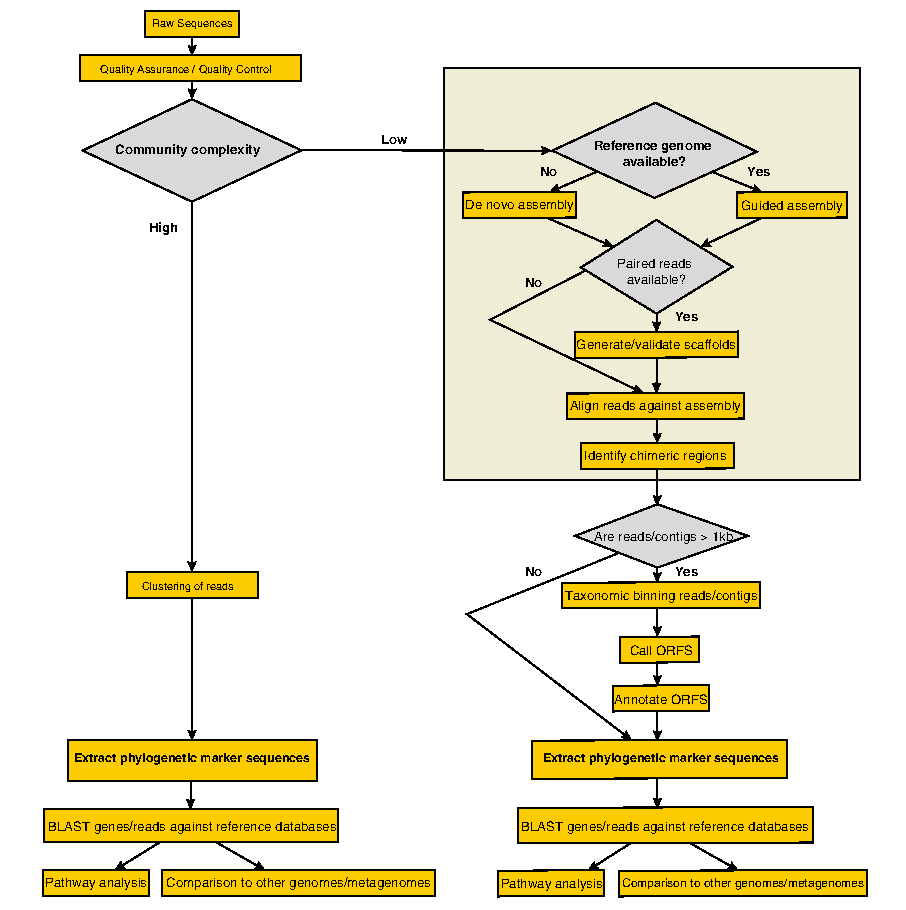
\includegraphics[width=\textwidth]{Chapter1/Figures/Metagenomics_GeneCentric_vs_Assembly.pdf}
	\caption{Diagram comparing two possible approaches for the analysis of metagenomic data from natural microbial communities. Figure from Bragg and Tyson, 2014 \cite{Bragg:2014kv}.}
	\label{MetagenomicComp}
\end{figure}

%\begin{figure}[!htbp]
%	\centering
%	*
%	\caption{Comparison of a set of reads (Illumin XXbp, total of XX reads) classified using Phylosift? with two different reference databases. The first case shows the reads classified in abscence of any reference genomes, the second one where reference genomes obtained through metagenomics \cite{Narasingarao:2012kp,Podell:2013kx} are included in the database}
%	\label{CompSeqClassification}
%\end{figure}

\section{Microbial communities in hypersaline environments}

Hypersaline habitats are found worldwide, in a variety of natural and man-made environments. Examples include salt lakes, saline soils, salt flats, solar salterns, brine pools, salted foods, and fermented foods \cite{Oren:2002vw}. Aquatic hypersaline systems are the most studied, and are either of marine origin (thalassohaline), or formed by the dissolution of mineral salt deposits (athalassohaline). 

Within these saline systems, a variety of microbial species are adapted to these environments. Moderate halophiles can beare found between 30-150 g/L NaCl, while extreme halophiles exist in the range of 150-300 g/L NaCl  \cite{Andrei:2012he}. In addition to the high NaCl concentrations, other salts are also important to consider when measuring the ionic composition of these systems, including Mg\textsuperscript{2+} and Ca\textsuperscript{2+}, which can inßuence the microbial community in these habitats  \cite{McGenity:2000ts,Podell:2013fp} (Figure \ref{IonicComposition}).

Genera from both the Bacteria and the Archaea exist in moderate and extreme saline systems. Within the Archaea, the phylogenetic diversity appears to be limited to the \textit{Euryarchaeota}, specifically in the classes \textit{Halobacteria} and \textit{Methanomicrobia} (Table \ref{TableArchaea}) \cite{Ventosa:2012wo}. The discovery of the \textit{Nanohaloarchaea} (described in Chapter 2, and \cite{Narasingarao:2012kp}), a novel Class, within the Euryarchaeota,, in globally dispersed hypersaline systems expanded our understanding of the phylogenetic diversity of halophilic Archaea \cite{Narasingarao:2012kp}. Recently, a phylogenomic analysis of novel archaeal groups, isolated via single-cell genomics, suggested that the \textit{Nanohaloarchaea} are a new phylum, sister to the \textit{Euryarchaeota} \cite{Rinke:2013bt}, although more work (and more genomes and isolates) is needed to fully resolve the phylogenetic relationships between these groups \cite{Williams:um}.

Even within the \textit{Halobacteria}, novel taxonomic groups remain unidentified. Our group recently described the genome of a newly isolated halophilic Archaea,  \textit{Candidatus} Halobonum tyrrellensis strain G22 \cite{Ugalde:2013hb}, which phylogenetic analysis suggests is a new genus within the \textit{Halobacteria} (Appendix \ref{G22Genome}). Analysis of the 16S rRNA gene, and a phylogenomic approach using the markers genes implemented in the software, PhyloPhlan, has further supported this phylogenetic placement (Figures \ref{G22_16Stree} \& \ref{G22_PhyloPhlanTree}).

The phylogenetic breadth of bacterial species found in saline systems is wider than that of Archaea (Table \ref{TableBacteria}). In moderate saline environments, Bacteria are more abundant than Archaea \cite{Oren:2008ej,Ghai:2011hn,Ghai:2012fb,Casamayor:2002tf}, but as salinity increases, Archaeal groups become more abundant \cite{Ghai:2011hn,Casamayor:2002tf,Mutlu:2008dk}. One of the most abundant bacterial species found in extreme hypersaline systems is \textit{Salinibacter ruber} \cite{Anton:2008eb}. This bacterium shares many phenotypic characteristics with halophilic Archaea \cite{Oren:2013gy}, and multiple gene clusters appear to have been acquired via horizontal gene transfer from the Archaea \cite{Mongodin:2005ie}.

Viruses are also very abundant in hypersaline systems, with reports of counts of at least \num{e7} viral-like particles per mL \cite{DyallSmith:2003eu}. Viruses could be playing a dual role in these systems; as predators, contributing to the cycling of nutrients through cell lysis; and as a form of information storage, by providing access to an auxiliary gene pool that can be utilized by other microorganisms \cite{Lindell:2005gz,Williamson:2008vs,Hurwitz:2013gl}.  Studies of viral dynamics in hypersaline systems have showed that they play a fundamental role in shaping the population structure of microbial communities \cite{RodriguezBrito:2010in,RodriguezValera:2009cr}.

Microorganisms that live in hypersaline systems require particular physiological strategies to deal with the high salt concentrations and the potential osmotic pressure gradient that can generate across the cell membrane. Two different osmotic adaptation strategies can be found in halophiles: a salt-in strategy, which involves the accumulation of inorganic ions in the cytoplasm; and a salt-out strategy, that involves pumping ions out the cell and the accumulation of compatible solutes in the cytoplasm \cite{Oren:2013bc}. The salt-in strategy is found in the archaeal populations, specifically within the Order \textit{Halobacteriales}, in Bacteria of the Order \textit{Halanerobiales} and in \textit{S. ruber} \cite{Oren:2013bc}. These organisms accumulate inorganic ions, such as K\textsuperscript{+} and Cl\textsuperscript{-}, which requires special enzymatic adaptations reflected through protein amino acid compositional changes that favor acidic amino acids, such as glutamate and aspartate. Based on their amino acid composition profiles, it has been suggested that the uncultured members of the Class \textit{Nanohaloarchaea} also utilize this strategy. The salt-out strategy is found in most of the halophilic Bacteria and halophilic methanogenic Archaea  \cite{Oren:2013bc}. These organisms have outward-directed sodium transporters that pump the Na\textsuperscript{+} ions out of the cytoplasm, but more importantly, they accumulate a large number of organic solutes to mantain the osmotic potential in the cytoplasm \cite{Oren:2013bc}.

Halophilic microorganisms show a diverse suite of metabolic capabilities. Several dissimilatory metabolic pathways have been described in halophiles (Figure \ref{HaloMetabolis}) across a wide range of salinity concentrations. The majority of bacterial and archaeal groups isolated from hypersaline sites are aerobic chemoorganotrophs. In addition, as oxygen has a low solubility in salt saturated brines \cite{Sherwood:1991tg}, several anaerobic energy pathways are available, including electron acceptor substrates such as nitrate, fumarate, and dimethyl sulfoxide \cite{Oren:2008ej,Oren:2013bc}. Primary productivity in saline systems varies according to the salinity. In moderate saline environments (between 100 to 250 g/L), primary productivity occurs in microbial mats dominated by members of the \textit{Cyanobacteria};  in high salt environments, the primary producers are planktonic algae of the genus \textit{Dunaliella} \cite{Oren:2009el}.

Another important characteristic of halophilic organisms, particularly among the halophilic Archaea, is the presence of microbial rhodopsins, photoactive proteins found in all three domains of life. Rhodopsins serve as light-driven proton pumps (bacteriorhodopsin), chloride pumps (halorhodopsin), or phototactic and photophobic receptors (sensory rhodopsins) \cite{Brown:2013ic}. Halorhodopsins and sensory rhodopsins appear to be limited in their distribution to the \textit{Halobacteria}, with just a few examples found in other organisms \cite{Sharma:2006kn}. Chapter 3 describes the discovery a novel type of microbial rhodopsin, called the xenorhodopsin, which was found in the genome of the \textit{Nanohaloarchaea}, and that appear to broadly dispered via horizontal gene transfer between Archaea and Bacteria (although it is not possible yet to establish the directionality of acquisition).Indeed, the closest homolog to the Nanohaloarchaea xenorhodopsin is a putative sensory rhodopsin found in the cyanobacterium \textit{Anabaena} sp. PCC 712 \cite{Vogeley:2004vh,Ugalde:2011fw}.

Even in highly characterized microbial communities  \cite{Oren:2008ej,Oren:2012bg}], recent studies using culture independent techniques, such as metagenomics and single-cell genomics, recovered novel microbial groups \cite{Narasingarao:2012kp,Ghai:2011hn,LopezPerez:2013db}. The limited microbial diversity, driven by extreme salinity systems, makes them ideal model systems to study microbial diversity using metagenomic methods. We can fully characterize a microbial community using deep-sequencing approaches, with the goal to reconstruct the genomes of each member of the community. Through this approach, we identify not only the functional and phylogenetic diversity of the community, but also the association of such functions to members of the community. Lastly, it allows for the study of population genetics within the community, with the goal of understanding how these organisms adapt and respond to variations in the environment.

It is important to highlight that other saline ecosystems have been studied using metagenomic approaches. Prior hypersaline metagenomic studies have focused on the population genomics of single species, such as \textit{Haloquadratum walsbyi} \cite{Legault:2006kh} and \textit{Salinibacter ruber} \cite{Pasic:2009bo}, or on the dynamic changes of the microbial and viral diversity over salinity gradientes and over time \cite{Willner:2009iv,RodriguezBrito:2010in}. Only recent studies have explored the microbial and viral diversity of these systems by using assembly-based metagenomics and single-cell genomics approaches \cite{Narasingarao:2012kp,Podell:2013kx,Ghai:2011hn,Ghai:2012fb,Emerson:2012gh,Emerson:tk}.

%FIGURE, G22 16S TREE
\begin{figure}[!htbp]
	\centering
	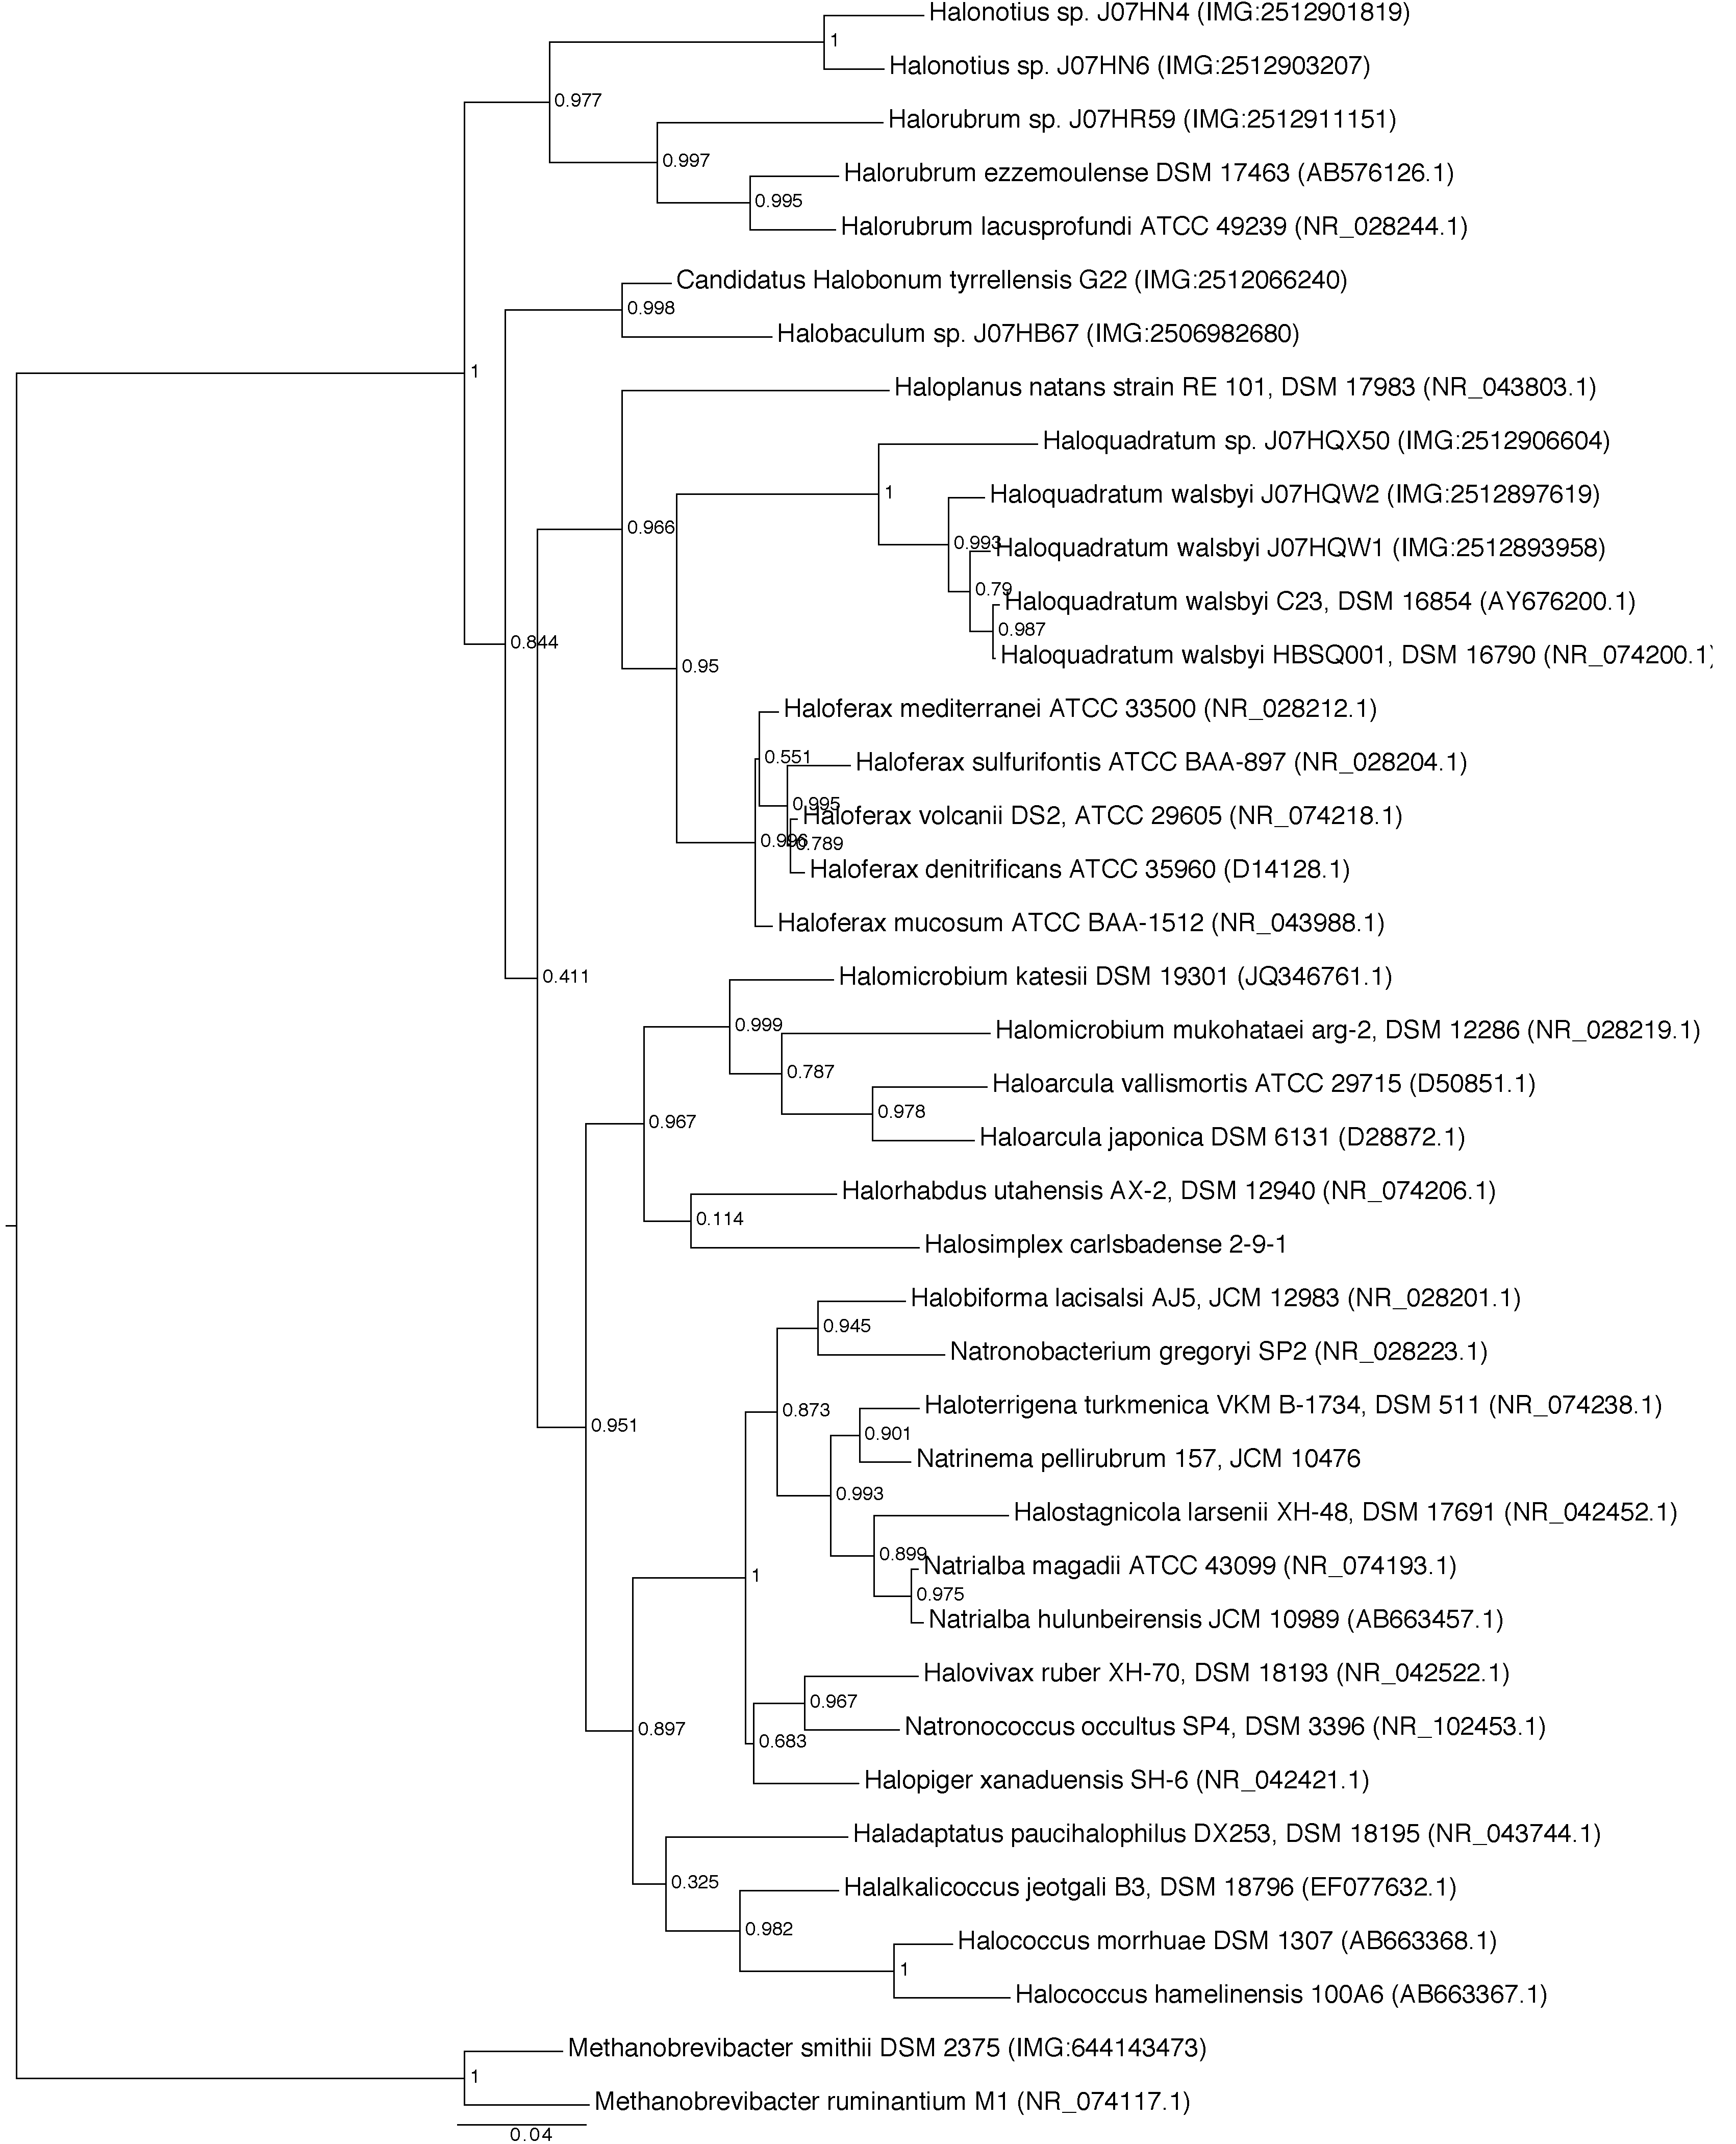
\includegraphics[width=\textwidth]{Chapter1/Figures/HaloG22_16S_v2-2.pdf}
	\caption{Phylogenetic tree of \textit{Candidatus} Halobonum tyrrellensis G22 and related microorganisms, based on 16S rRNA sequences.}
	\label{G22_16Stree}
\end{figure}

%FIGURE, G22, PHYLOPHLA TREE
\begin{figure}[!htbp]
	\centering
	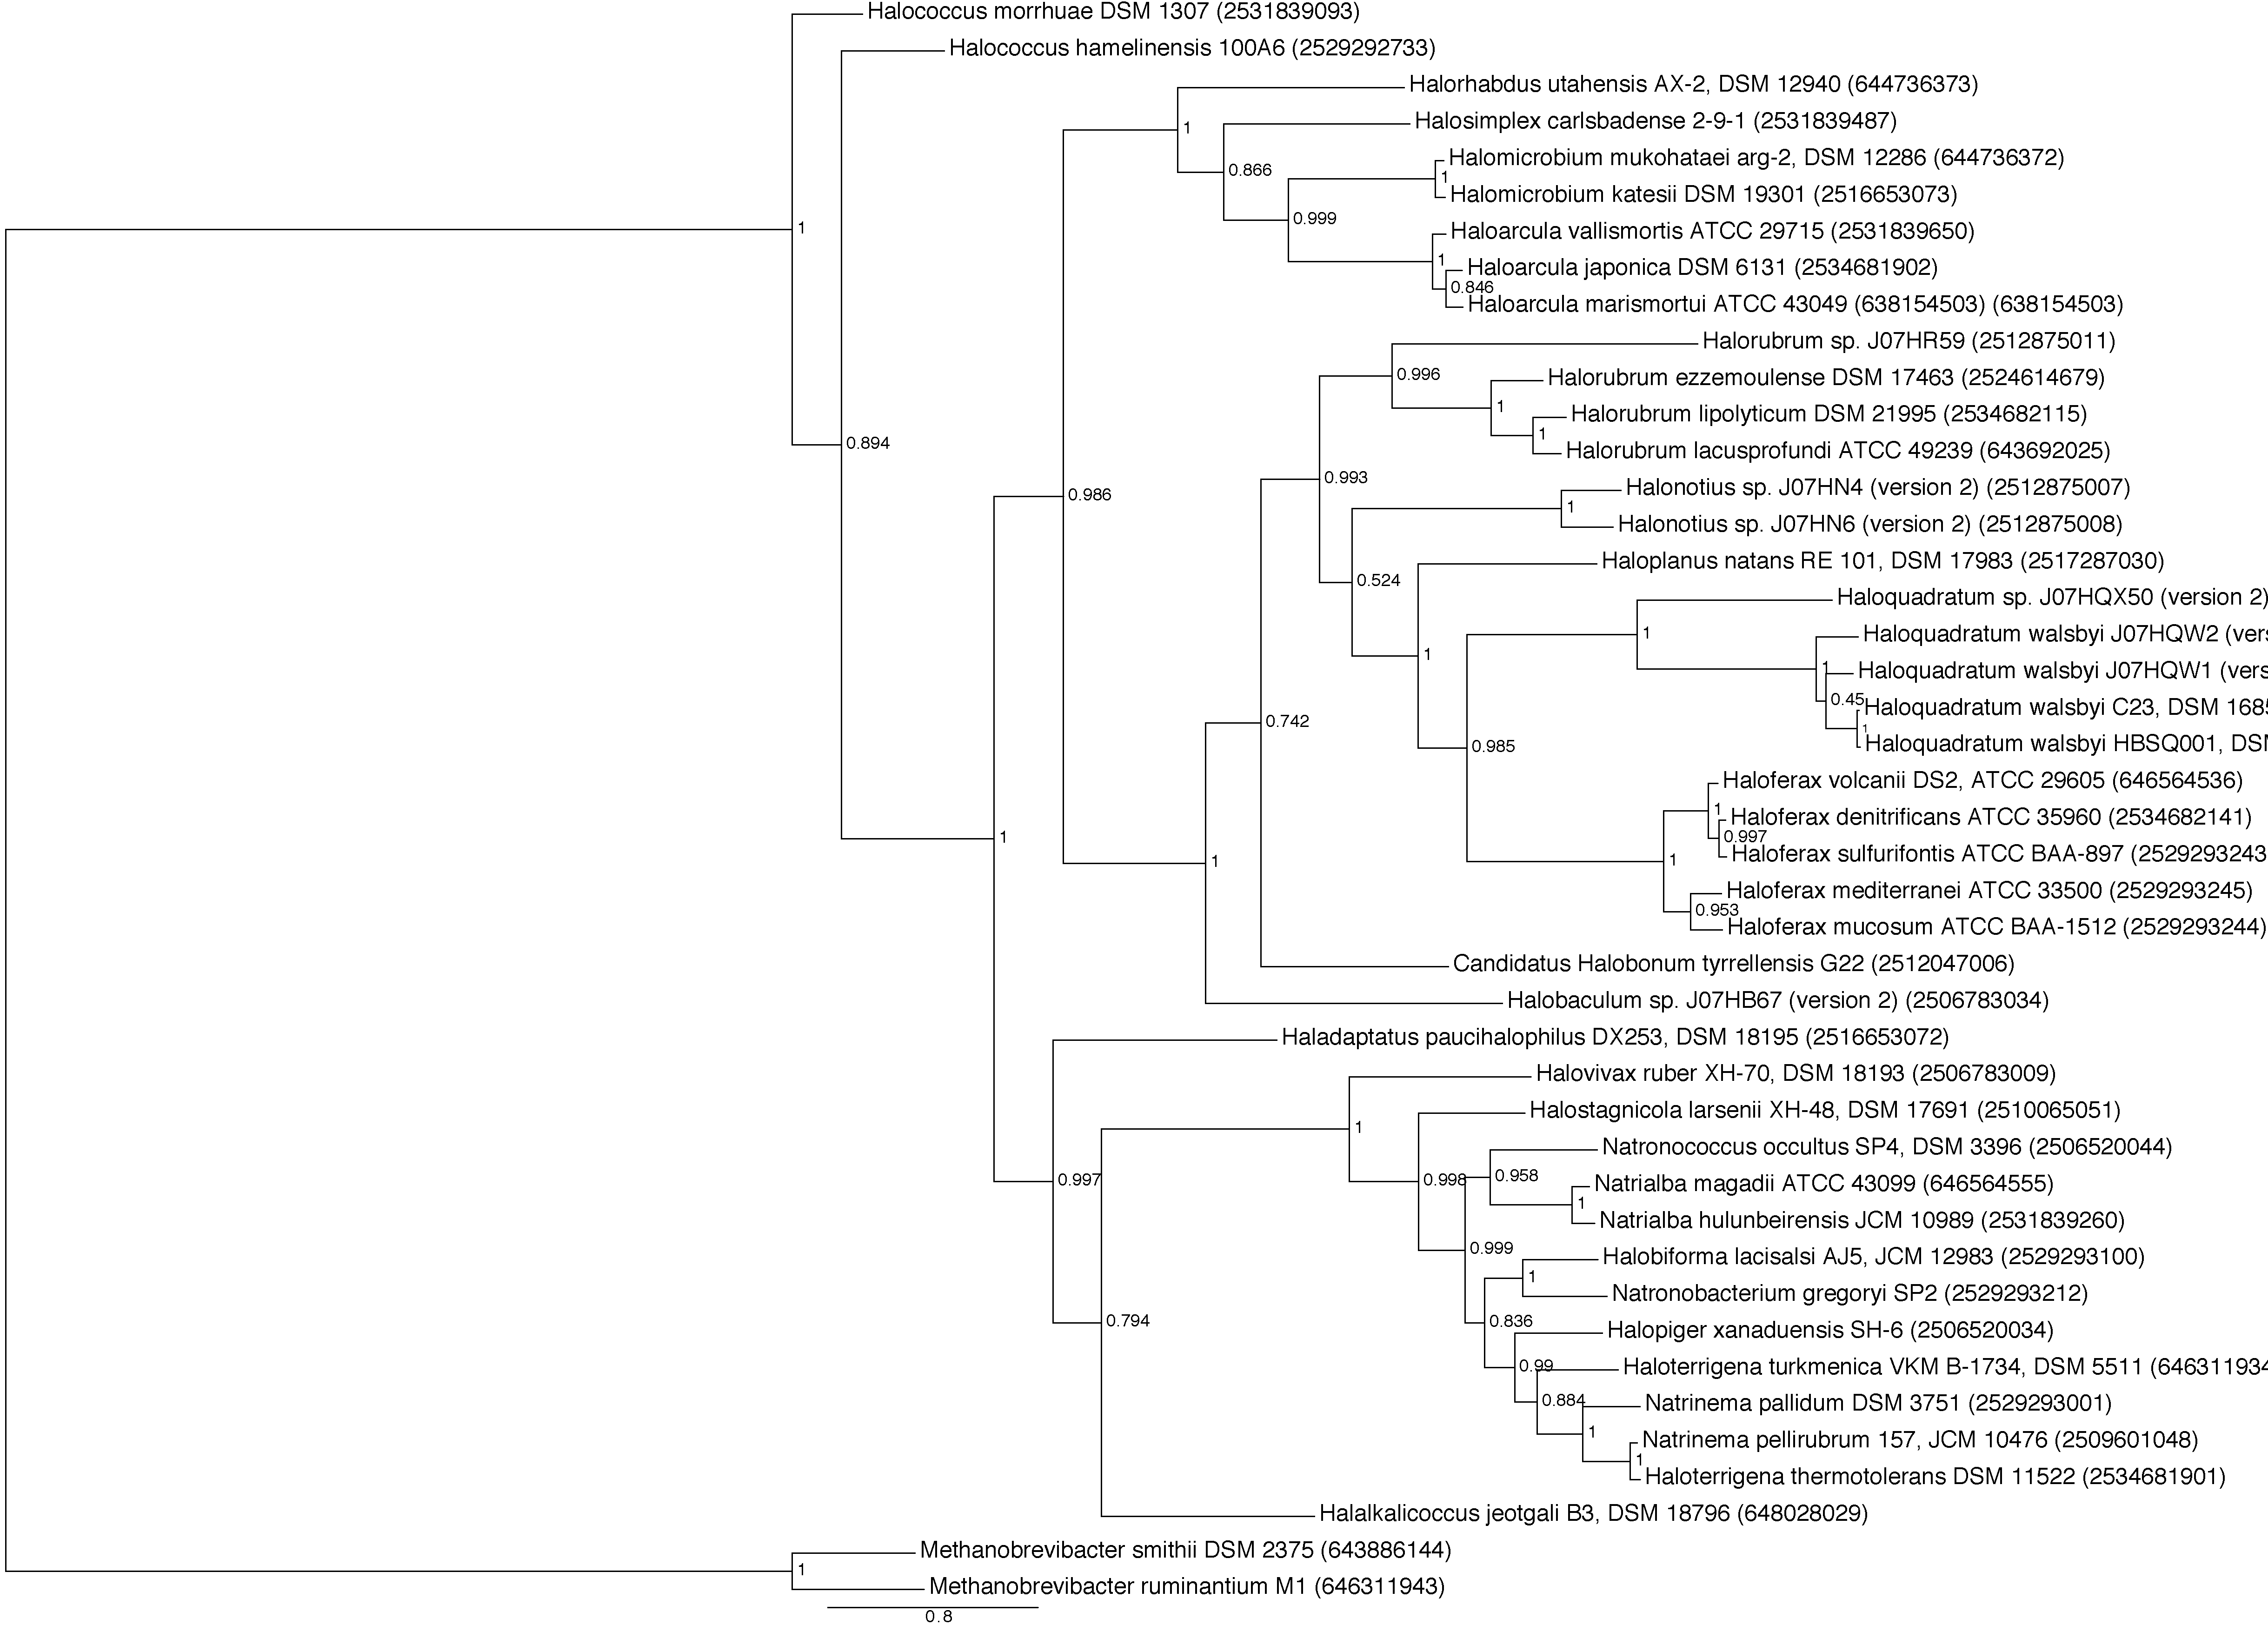
\includegraphics[width=\textwidth]{Chapter1/Figures/HaloG22_v6.pdf}
	\caption{Phylogenetic tree of \textit{Candidatus} Halobonum tyrrellensis G22 and related microorganisms, based on phylogenetic marker sequences implemented in the Phylophlan software \cite{Segata:2013hb}}
	\label{G22_PhyloPhlanTree}
\end{figure}

%FIGURE IONIC COMPOSITION
\begin{figure}[!htbp]
	\centering
	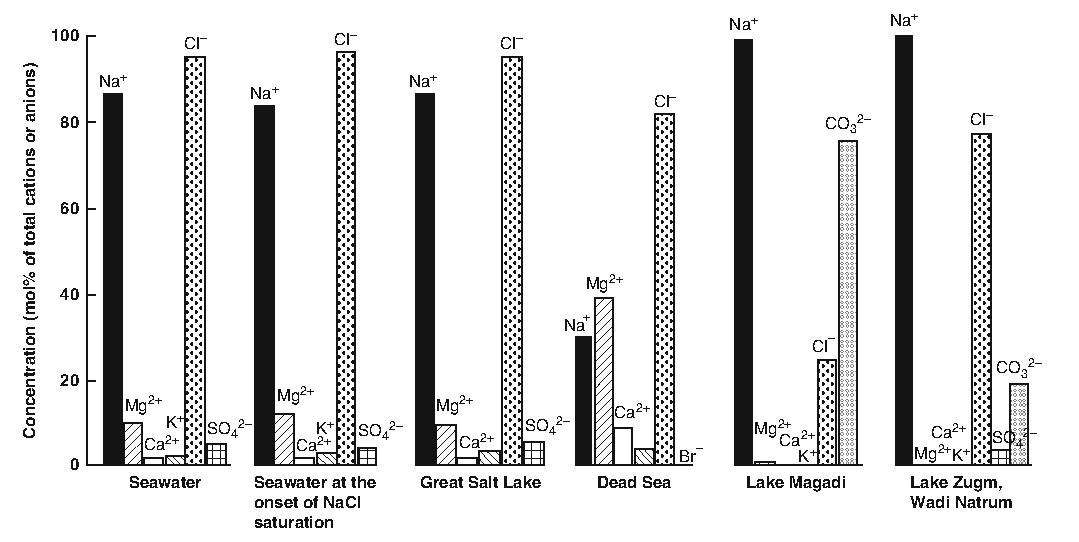
\includegraphics[width=\textwidth]{Chapter1/Figures/IonicComposition.pdf}
	\caption{Ionic composition of several aquatic systems. Figure from Oren, 2013. \cite{Oren:2013bc}}
	\label{IonicComposition}
\end{figure}

%FIGURE IONIC COMPOSITION
\begin{figure}[!htbp]
	\centering
	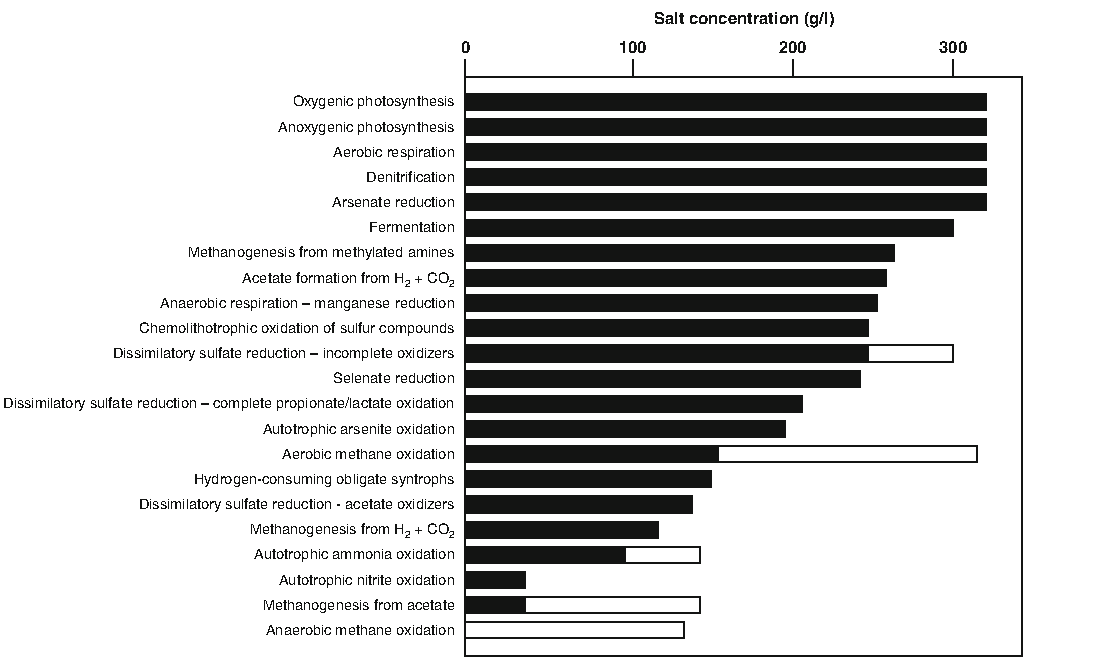
\includegraphics[width=\textwidth]{Chapter1/Figures/HaloMetabolism.pdf}
	\caption{Salt concentration limits for some microbial metabolic processes. Black bars indicate information based on laboratory studies, while white bars indicate activities measured in natural microbial communities. Figure from Oren, 2013 \cite{Oren:2013bc}.}
	\label{HaloMetabolis}
\end{figure}


%TABLE, ARCHAEA DIVERSITY
\begin{table}[!htdp]
\caption{Halophilic Archaea, modified from \cite{Ventosa:2012wo} to include the recently discovered \textit{Nanohaloarchaea} \cite{Narasingarao:2012kp}.}
\begin{center}

\resizebox{\textwidth}{!}{%
\begin{tabularx}{\textwidth}{p{3cm} p{3cm} X}
\hline
\textbf{Phylum} & \textbf{Class} & \textbf{Genera} \\
\hline
\textit{Euryarchaeota} & \textit{Halobacteria} & \textit{Halobacteria, Haladaptatus, Halalkalicoccus, Halarchaeum, Haloarcula, Halobaculum, Halobiforma, Halococcus, Haloferax, Halogeometricum, Halogranum, Halomicrobium, Halonotius, Halopelagius, Halopiger, Haloplanus, Haloquadratum, Halorhabdus, Halorubrum, Halorussus, Halosarcina, Halosimplex, Halostagnicola, Haloterrigena, Halovivax, Natrialba, Natrinema, Natronoarchaeum, Natronobacterium, Natronococcus, Natronolimnobius, Natronomonas, Natronorubrum, Salarchaeum} \\
\cline{2-3} 
& \textit{Methanomicrobia} & \textit{Methanohalobium, Methanocalculus, Methanohalohilus, Methanosalsum} \\
\hline
\textit{Nanohaloarchaea} &  & \textit{Nanosalina, Nanosalinarum} \\
\end{tabularx}
}

\end{center}
\label{TableArchaea}
\end{table}




%TABLE BACTERIA DIVERSITY
\begin{center}

\begin{longtable}{p{3cm} p{4.5cm} p{5.5cm}}
\label{TableBacteria}\\
\caption{Halophilic Bacteria, modified from \cite{Ventosa:2012wo}.}\\

\hline
\textbf{Phylum} & \textbf{Class} & \textbf{Genera} \\
\hline
\endfirsthead

\multicolumn{3}{c}%
{\tablename\ \thetable\ -- \textit{Continued from previous page}} \\
\hline
\textbf{Phylum} & \textbf{Class} & \textbf{Genera} \\
\hline
\endhead

\hline \multicolumn{3}{r}{\textit{Continued on next page}} \\
\endfoot
\hline
\endlastfoot


\textit{Actinobacteria} & \textit{Actinobacteria} & \textit{Actinopolyspora, Amycolatopsis, Georgenia, Corynebacterium, Haloactinobacterium, Haloactinopolyspora, Haloechinothrix, Haloglycomyces, Nesterenjonia, Nocardiopsis, Haloactinospora, Streptomonospora, Isoptericola, Prauserella, Saccharomonospora, Saccharopolyspora} \\
\hline

\textit{Bacteroidetes} & \textit{Bacteroidia} & \textit{Anaerophaga} \\
\cline{2-3}

& \textit{Flavobacteria} & \textit{Gramella, Psychroflexus} \\
\cline{2-3}
& \textit{Sphingobacteria} & \textit{Salinibacter, Salisaeta} \\
\hline

\textit{Cyanobacteria} & & \textit{Rubidibacter, Prochlorococcus, Halospirulina} \\
\hline

\textit{Firmicutes} & \textit{Bacilli} & \textit{Alkalibacillus, Aquisalibacillus, Bacillus, Filobacillus, Gracilibacillus, Halalkalibacillus, Halolactibacillus, Halobacillus, Jeotgalibacillus, Lentibacillus, Oceanobacillus,Ornithinibacillus, Paraliobacillus, Piscibacillus, Pontibacillus, Salimicrobium, Salinibacillus, Salirhabdus, Salsuginibacillus, Sediminibacillus, Salinicoccus, Tenuibacillus, Thalassobacillus, Virgibacillus} \\
\cline{2-3}
& \textit{Clostridia} & \textit{Acetohalobium, Halanaerobacter, Halanaerobium, Halobacteroides, Halocella, Halonatronum, Halothermothrix, Natranaerobius, Natrionella, Natronovirga, Orenia, Selenihalanaerobacter, Sporohalobacter} \\
\hline

\textit{Proteobacteria} & \textit{Alphaproteobacteria} & \textit{Antarctobacter, Citreimonas, Dichotomicrobium, Fodinicurvata, Hwanghaeicola, Hyphomonas, Jannaschia, Maribaculum, Maribius, Marispirillum, Methylarcula, Oceanibulbus, Oceanicola, Palleronia, Paracoccus, Ponticoccus, Rhodobium, Rhodotalassium, Rhodovibrio, Rhodovulum, Roseicitreum, Roseinatronobacter, Roseisalinus, Roseospira, Roseovarius, Salinihabitans, Salipiger, Sediminimonas, Shimia, Sulfitobacter, Tropicibacter, Woodsholea, Yangia} \\
\cline{2-3}
& \textit{Gammaproteobacteria} & \textit{Aidingimonas, Alcanivorax, Alkalilmnicola, Alteromonas, Aestuariibacter, Aquisalimonas, Arhodomonas, Carnimonas, Chromohalobacter, Cobetia, Ectothiorhodspira, Ectothiorhodosinus, Glaciecola, Gilvimarinus, Haliea, Halochromatium, Halomonas, Halorhodospira, Halospina, Halothiobacillus, Idiomarina, Kushneria, Marichromatium, Marinobacter, Marinobacterium, Melitea, Methylohalomonas, Microbulbifer, Modicisalibacter, Nitrincola, Oleispira, Pseudidiomarina, Pseudoaltermonas, Psychromonas, Pseudomonas, Saccarospirillum, Salicola, Salinicola, Salinisphaera, Salinivibrio, Thioalkalibacter, Thioalkalivibrio, Thiohalobacter, Thiohalorhabdus, Thiohalocapsa, Thiohalomonas, Thiohalophilus, Thiohalospira, Thiomicrospira} \\
\cline{2-3}
& \textit{Deltaproteobacteria} & \textit{Desulfocella, Desulfohalobium, Desulfonatronospira, Desulfosalsimonas, Desulfovermiculus, Desulfovibrio, Desulfurivibrio} \\
\cline{2-3}
& \textit{Epsilonproteobacteria} & \textit{Arcobacter, Sulfurimonas, Sulfurovum} \\
\hline

\textit{Spirochaetes} & \textit{Spirochaetes} & \textit{Spirochaeta} \\
\hline

\textit{Tenericutes} & \textit{Mollicutes} & \textit{Haloplasma} \\
\hline

\textit{Thermotogae} & \textit{Thermotogae} & \textit{Petrotoga} \\

\end{longtable}

\end{center}





\section{Lake Tyrrell, Australia, as a model ecosystem}

Lake Tyrrell, Victoria, Australia, is located in the center of the Murray Basin Plains (Figure \ref{LT_map}), in a region with a semi-arid climate, average rainfall of 300 mm/year, and an evaporation rate of ~2000 mm/year  \cite{Macumber:1992ty}. The lake is considered an acid-hypersaline system, where low-pH, oxygenated, saline, metal-rich groundwater from springs is evapo-concentrated and mixed with near-neutral pH waters, rich in sulfides \cite{Long:1992ie}. The lake shows seasonal salinity variations. During winter, the salt content is approximately  \textgreater 250 g/L; in summer, due to water evaporation, the residual brines reach concentrations \textgreater 330 g/L \cite{Macumber:1992ty}.

Lake Tyrrell has been described and studied in detail in terms of its hydrological and geochemical features  \cite{Long:1992ie,Macumber:1992ty,Jones:2006jn}], making it a great candidate for microbiological characterization. Recent projects have used a diverse array of microbiological techniques to study the microbial diversity of Lake Tyrrell, including Eukaryotes \cite{KarlaBHeidelberg:2013jc}, Archaea and Bacteria \cite{Podell:2013kx,Narasingarao:2012kp,Ugalde:2013hb}, and Viruses \cite{Emerson:2012gh,Emerson:tk}. Future work will combine the metagenomic, proteomic, and available geochemical information to provide a more integrative description of the interactions between microbes, viruses, and the environment. 

In this thesis, we explore the microbial diversity of the Lake Tyrrell ecosystem, based on the data generated through a metagenomic study. In particular, our study highlights how, by assembling metagenomic data, we obtain a more complete picture of the microbial diversity present in the community, and also how we can exploit this information to obtain a broad picture of the phylogenetic and functional diversity, and to explore in detail the genetic diversity of the members of the microbial community.

\textbf{Chapter 2} describes how the assembly of metagenomic datasets allowed the recovery and identification of novel microbial groups that are abundant in the hypersaline waters of Lake Tyrrell, and other hypersaline ecosystems. Using additional metadata, such as size fractionation, sequence nucleotide composition, and phylogenetic binning, two near-complete genomes from a novel Class of Archaea, the \textit{Nanohaloarchaea}, were recovered from the metagenomic samples. . This chapter represents work that has already been published  \cite{Narasingarao:2012kp}. My role, in this study was in the classification of sequences into phylogenetic groups using statistical approaches, such as non-metric multidimensional scaling, and exploring the functional diversity of the two novel genomes.

\textbf{Chapter 3} corresponds to the bioinformatic analysis and description of a novel type of microbial rhodopsin, xenorhodopsin, identified from the genomes of the Nanohaloarchaea.The results convey how this rhodopsin appears to be a new class of microbial rhodopsin based on phylogenetic analysis and on the presence of unique amino acid signatures. This work has already been published \cite{Ugalde:2011fw}, where I was the lead author of the study. 

\textbf{Chapter 4} describes the assembly of several genomes from the Lake Tyrrell metagenome, based on the combination of assembly-based approaches and metadata. These results provide a framework for future analyses of this ecosystem, providing a set of habitat-specific genomes, including phylogenetic, functional, and genetic diversity. This work is already published \cite{Podell:2013kx}. My role in this study was developing the methods for classification of the assembled scaffolds into different phylogenetic groups and developing novel visualization and analysis approaches to compare the functional repertoire of community members.

\textbf{Chapter 5}, leverages the assembled habitat-specific genomes, and describes a bioinformatic approach for the analysis of genetic diversity using metagenomic approaches. Using this framework, a deep-sequencing approach was used to characterize the population composition and genetic heterogeneity of two different temporal samples (Summer and Winter) from the microbial members of the Lake Tyrrell community.

%FIGURE LT MAP
\begin{figure}[!htbp]
	\centering
	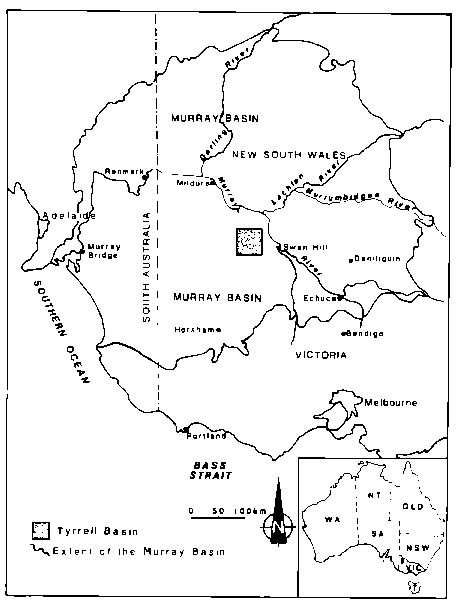
\includegraphics[width=\textwidth]{Chapter1/Figures/LT_Map.pdf}
	\caption{Location of Lake Tyrrell in the southeastern region of Australia. Figure from Macumber, 1992. \cite{Macumber:1992ty}.}
	\label{LT_map}
\end{figure}


%   \include{chapter2}
%
% Of course, if you prefer, you can just start with
%   \chapter{My First Chapter Name}
% and start typing away. 

%Chapter 1

\chapter{Introduction to the thesis}

    Bacteria and Archaea represent an abundant component of Earth's biomass, with estimates between 9.2-31.7 \num{e29} cells \cite{Kallmeyer:2012km} to 41.8-64.3 \num{e29} cells \cite{Whitman:1998tj} globally. Species diversity estimates suggest that there are close to \num{e7} different species of Bacteria and Archaea\cite{Curtis:2002dj}, although some authors suggest this number is an over-estimation \cite{Schloss:2004do}. Nevertheless, Bacteria and Archaea represent the most diverse group of organisms on Earth, and yet we have scarcely begun to characterize this diversity \cite{Wu:2009ju, Rinke:2013bt}.

    Our inability to cultivate most of the microorganisms present in the environment limits our understanding of the phylogenetic and functional diversity of microbial communities. Known as the "Great Plate-Count Anomaly" \cite{Staley:1985ww}, our current culture collections may not be representative of what can be observed in natural samples by culture-independent methods \cite{Amann:1995tw}. Most organisms are currently uncultured, due to our lack of information on their physiology and nutritional requirements \cite{Stewart:2012dd}. With new and unique cultivation methods, and information derived from genomic surveys \cite{Tyson:2005by}, we may be able to culture these organisms in the near future.
    
   Over the last decade, the development of advanced technologies and experimental methods has allowed the study of natural microbial communities via culture-independent techniques. Specifically, DNA-based methods, driven by the development of next-generation sequencing \cite{Mardis:2008fr}, have allowed the investigation of natural microbial communities without relying on cultivation. DNA-based surveys span two broad categories: marker-based analysis (such as the 16S rRNA gene) and whole genome sequencing.
    
    Marker-based analysis provides a characterization,or census, of the phylogenetic diversity present in the community, allowing for estimation of community diversity\cite{Caporaso:2011cs, Rappe:2003fc, Caporaso:2010bi} and identification of community members based on sequence similarity against a reference database  \cite{McDonald:2011hn}. This approach provides only a partial picture of the metabolic repertoire present in natural microbial communities, as it requires extrapolation of genomic data from isolated microorganisms to the entire community. Even strains with very similar 16S rRNA sequences may have different metabolic and genetic properties, which are not captured in the diversity found using a marker gene such as the 16S rRNA gene \cite{Jaspers:2004ge}.
    
    Metagenomics, also referred to as community genomics, relies on the direct sequencing of genetic material isolated from a microbial community \textit{en masse} \cite{Wooley:2010uv}, and provides the means to evaluate the phylogenetic and functional diversity of microbial populations directly from the environment. Depending on the complexity of the community under study, not all of the members of the microbial community will be observed in the sequence data, as the most abundant members will dominate the metagenomic analyses \cite{Bragg:2014kv}. Using metagenomic methods, several authors report studies of microbial communities with low to moderate species diversity  (e.g. \cite{Ugalde:2013he,Podell:2013kx,Dinsdale:2008cd,Tyson:2004bw,Brulc:2009fi}). Highly diverse communities, such as those found in soils and sediments, require high amounts of sequence information to provide a full picture of the microorganisms that are present \cite{Kakirde:2010ew}. The decrease in sequencing cost, driven by the development of novel sequencing technologies, has enhanced our ability to deeply sample complex communities using metagenomics approaches. Consequently, the challenge will be developing or acquiring the computational resources and algorithms necessary to analyze vast amounts of genetic sequence information  \cite{Pell:2012id,Kakirde:2010ew}. 
    
    Microbial communities in extreme environments, such as those associated with hypersaline habitats, represent tractable systems that can be studied using metagenomic approaches. Because of their relatively low species diversity  \cite{Andrei:2012he,Podell:2013kx,Ghai:2011hn}, it is possible to study the phylogenetic and metabolic diversity that is present in the community. In this first chapter, I provide an overview of metagenomics, with particular emphasis in assembly-based approximations, followed by an introduction into the microbiology of hypersaline environments and finally an overview of our study site, the hypersaline waters of Lake Tyrrell located in Victoria, Australia.

\section{Metagenomics}

    The study of natural microbial communities by analyzing DNA obtained directly from environmental samples was first proposed by Handelsman \textit{et al.} in 1998 \cite{Handelsman:1998tx} to access the genomic information of uncultured environmental microorganisms. The first metagenomic studies were performed by isolating DNA from environmental samples, plasmid-based cloning of this DNA and subsequence sequencing of these clones using the Sanger method \cite{Tyson:2004bw,Venter:2004hg}. Limited throughput, cloning biases, and the expesive and laborious nature of this process limited the scope of early metagenomic studies, often focused on microbial communities with low to medium species diversity \cite{Tyson:2004bw,Podell:2013kx}, or to studies aimed at describing the general functional and phylogenetic composition of a community  \cite{Venter:2004hg,Rusch:2007ez}. The development of \textit{next generation} sequencing technologies \cite{Mardis:2013gn}, removed some of these limitations, allowing for direct sequencing of DNA samples without cloning,  higher throughputs, and a lower cost per base \cite{Mardis:2013gn}. One of the remaining limitations in current technologies is the length of the sequence reads, which are not yet close to the length of reads generated by Sanger sequencing. Improvements to current methods and the development of further advanced technologies, such as single molecule sequencing \cite{Eid:2009kv} and nanopores \cite{Branton:2008fr}, holds promise to further alleviate these limitations.

Metagenomic studies are driven, in most cases, by discovery, data mining and comparative research, rather than by a specific hypothesis \cite{Wooley:2010uv}. Accordingly, both the sequence information and the contextual environmental data, or metadata, associated with a sample are of great importance, allowing for both biological and physicochemical context to be applied to the microbial community under study. These data include environmental parameters associated with a sample and procedures used to process a sample (e.g. filtration procedure, sample processing and library construction). All of these variables become highly important in the bioinformatic analysis of a sample data set\cite{Narasingarao:2012kp}.

Based on the complexity of the microbial community under study, and the choice of sampling and sequencing methods, two main approaches are used to study microbial communities using metagenomics: gene-centric and assembly-based approaches  (Figure \ref{MetagenomicComp}). 
Gene-centric studies focus on complex communities or projects with a shallow level of sequencing, where assembly of larger contiguous genome fragments from community members is not feasible given the number of reads or size of the data set obtained. . In these cases, the focus is on the phylogenetic and functional diversity as a profile of the community \cite{Ugalde:2013he,Brulc:2009fi}, and the comparison of different environments based on these profiles \cite{Dinsdale:2008cd,Willner:2009iv,Reed:2014jj}. Gene-centric studies focus on the phylogenetic and functional classification of the metagenomic reads, either by analyzing every read present in the dataset \cite{Brady:2011hi,Parks:2011bh,AmritaPati:2011ba}, or by using marker-genes as a proxy to create either taxonomic and/or functional profiles of the community \cite{Darling:2014ej,Segata:2012ba}.  One main drawbacks of this method is that community profiles are limited by the reference databases being used, which can lead to missing unique groups that are present in the microbial community under study. 

%For example, Figure \ref{CompSeqClassification} shows the results of classifying a set of metagenomic reads using two different reference databases. In this example, the query reads were obtained from a sample obtained from the hypersaline surface waters of Lake Tyrrell, sequenced on the Illumina HiSeq platform (XX reads, XX average length). Two different reference databases were used, implemented in the Phylosift \cite{Darling:2014ej} package; one where the genome of organisms know to be present in the Lake Tyrrell sample were included, and a second database where these genomes were absent. 
%\todo{Complete Phylosift results}

Assembly-based metagenomics, involves the bioinformatic assembly of the community sequence information, with the goal of recovering larger contiguous genome fragments that can improve the phylogenetic and functional classification of the organisms in the community. This approach allows the recovery of longer fragments, generate better gene models and can identify previously unknown microbial groups \cite{Narasingarao:2012kp,Podell:2013kx,Kantor:2013ir,DiRienzi:2013kx}. The information obtained from the assembled population genomes can be used to potentially guide cultivation efforts for these organisms \cite{Tyson:2005by}, in population genetic studies \cite{Simmons:2008by,Ward:2008hp,Allen:2007ju}, and provide a better picture of the interactions among the members of the microbial community \cite{Tyson:2004bw,Flowers:2013hq}. In addition, the recovery of near-complete genomes from metagenomics datasets allows for the discovery of novel functions that may be missed by viewing the unassembled sequence reads. For example, Chapter 2 of this thesis shows how the assembly of sequence reads from the Lake Tyrrell metagenome led to the discovery of a previously unknown Phylum of Archaea and to the discovery of a novel family of microbial rhodopsins, called the xenorhodopsins, and evidence that suggests its acquisition through horizontal gene transfer (Chapter 3).

Assembly-based methods are limited by the complexity of the microbial community under study, and the amount of sequencing needed to recover the genomes of the most abundant members of the community. Furthermore, some of the more rare members of the community are inaccessible by sequencing, because the most abundant organisms dominate the metagenomic dataset.  For example, estimations of the number of sequences needed to address highly diverse samples, such as from soils, show that billions of sequences are needed to be able to sample some of these most abundant organisms \cite{Howe:2014go}. Even in simpler systems, the main challenge is to classify the assembled genomic fragments into unique phylogenetic bins, each representing a different population. By combining various pieces of information, such as sample characteristics, nucleotide composition, amino acid counts, and library abundance, it is possible to classify these genomic fragments into unique populations, a process known as phylogenetic binning \cite{Podell:2013kx,Albertsen:2013gp}. Larger datasets represent a computational challenge because of the high memory requirements of short-read assembly software programs. In this case, the use of methods for digital normalization may reduce the computational problems \cite{Pell:2012id,Kakirde:2010ew}.

The work presented in this thesis describes a study of the microbial community inhabiting the hypersaline waters of Lake Tyrrell, Australia using an assembly-based approach. The combination of a relatively low-species diversity, driven by the extreme conditions found in this habitat  \cite{Andrei:2012he}, and a deep sequencing approach, allowed for the genomic reconstruction of some of the most abundant members of the community and the discovery of novel microorganisms.

%CLASSIFICATION (Using Kraken)
%This is for the datasets without the reference genomes (LT)
%17165688 sequences (1089.97 Mbp) processed in 394.493s (2610.8 Kseq/m, 165.78 Mbp/m).
%  834490 sequences classified (4.86\%)
%  16331198 sequences unclassified (95.14\%)
%  
%Minikraken
%17165688 sequences (1089.97 Mbp) processed in 57.766s (17829.5 Kseq/m, 1132.12 Mbp/m).
%  806895 sequences classified (4.70%)
%  16358793 sequences unclassified (95.30%)
%
%Classification (phylosift?)

\begin{figure}[!htbp]
	\centering
	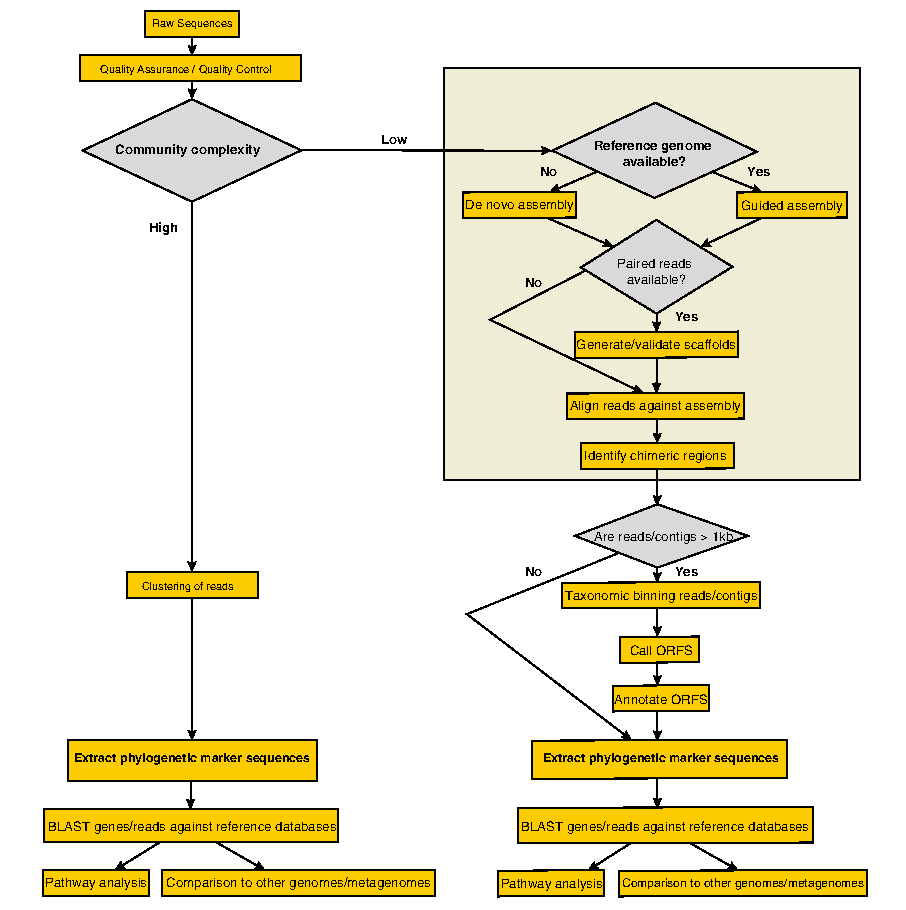
\includegraphics[width=\textwidth]{Chapter1/Figures/Metagenomics_GeneCentric_vs_Assembly.pdf}
	\caption{Diagram comparing two possible approaches for the analysis of metagenomic data from natural microbial communities. Figure from Bragg and Tyson, 2014 \cite{Bragg:2014kv}.}
	\label{MetagenomicComp}
\end{figure}

%\begin{figure}[!htbp]
%	\centering
%	*
%	\caption{Comparison of a set of reads (Illumin XXbp, total of XX reads) classified using Phylosift? with two different reference databases. The first case shows the reads classified in abscence of any reference genomes, the second one where reference genomes obtained through metagenomics \cite{Narasingarao:2012kp,Podell:2013kx} are included in the database}
%	\label{CompSeqClassification}
%\end{figure}

\section{Microbial communities in hypersaline environments}

Hypersaline habitats are found worldwide, in a variety of natural and man-made environments. Examples include salt lakes, saline soils, salt flats, solar salterns, brine pools, salted foods, and fermented foods \cite{Oren:2002vw}. Aquatic hypersaline systems are the most studied, and are either of marine origin (thalassohaline), or formed by the dissolution of mineral salt deposits (athalassohaline). 

Within these saline systems, a variety of microbial species are adapted to these environments. Moderate halophiles can beare found between 30-150 g/L NaCl, while extreme halophiles exist in the range of 150-300 g/L NaCl  \cite{Andrei:2012he}. In addition to the high NaCl concentrations, other salts are also important to consider when measuring the ionic composition of these systems, including Mg\textsuperscript{2+} and Ca\textsuperscript{2+}, which can inßuence the microbial community in these habitats  \cite{McGenity:2000ts,Podell:2013fp} (Figure \ref{IonicComposition}).

Genera from both the Bacteria and the Archaea exist in moderate and extreme saline systems. Within the Archaea, the phylogenetic diversity appears to be limited to the \textit{Euryarchaeota}, specifically in the classes \textit{Halobacteria} and \textit{Methanomicrobia} (Table \ref{TableArchaea}) \cite{Ventosa:2012wo}. The discovery of the \textit{Nanohaloarchaea} (described in Chapter 2, and \cite{Narasingarao:2012kp}), a novel Class, within the Euryarchaeota,, in globally dispersed hypersaline systems expanded our understanding of the phylogenetic diversity of halophilic Archaea \cite{Narasingarao:2012kp}. Recently, a phylogenomic analysis of novel archaeal groups, isolated via single-cell genomics, suggested that the \textit{Nanohaloarchaea} are a new phylum, sister to the \textit{Euryarchaeota} \cite{Rinke:2013bt}, although more work (and more genomes and isolates) is needed to fully resolve the phylogenetic relationships between these groups \cite{Williams:um}.

Even within the \textit{Halobacteria}, novel taxonomic groups remain unidentified. Our group recently described the genome of a newly isolated halophilic Archaea,  \textit{Candidatus} Halobonum tyrrellensis strain G22 \cite{Ugalde:2013hb}, which phylogenetic analysis suggests is a new genus within the \textit{Halobacteria} (Appendix \ref{G22Genome}). Analysis of the 16S rRNA gene, and a phylogenomic approach using the markers genes implemented in the software, PhyloPhlan, has further supported this phylogenetic placement (Figures \ref{G22_16Stree} \& \ref{G22_PhyloPhlanTree}).

The phylogenetic breadth of bacterial species found in saline systems is wider than that of Archaea (Table \ref{TableBacteria}). In moderate saline environments, Bacteria are more abundant than Archaea \cite{Oren:2008ej,Ghai:2011hn,Ghai:2012fb,Casamayor:2002tf}, but as salinity increases, Archaeal groups become more abundant \cite{Ghai:2011hn,Casamayor:2002tf,Mutlu:2008dk}. One of the most abundant bacterial species found in extreme hypersaline systems is \textit{Salinibacter ruber} \cite{Anton:2008eb}. This bacterium shares many phenotypic characteristics with halophilic Archaea \cite{Oren:2013gy}, and multiple gene clusters appear to have been acquired via horizontal gene transfer from the Archaea \cite{Mongodin:2005ie}.

Viruses are also very abundant in hypersaline systems, with reports of counts of at least \num{e7} viral-like particles per mL \cite{DyallSmith:2003eu}. Viruses could be playing a dual role in these systems; as predators, contributing to the cycling of nutrients through cell lysis; and as a form of information storage, by providing access to an auxiliary gene pool that can be utilized by other microorganisms \cite{Lindell:2005gz,Williamson:2008vs,Hurwitz:2013gl}.  Studies of viral dynamics in hypersaline systems have showed that they play a fundamental role in shaping the population structure of microbial communities \cite{RodriguezBrito:2010in,RodriguezValera:2009cr}.

Microorganisms that live in hypersaline systems require particular physiological strategies to deal with the high salt concentrations and the potential osmotic pressure gradient that can generate across the cell membrane. Two different osmotic adaptation strategies can be found in halophiles: a salt-in strategy, which involves the accumulation of inorganic ions in the cytoplasm; and a salt-out strategy, that involves pumping ions out the cell and the accumulation of compatible solutes in the cytoplasm \cite{Oren:2013bc}. The salt-in strategy is found in the archaeal populations, specifically within the Order \textit{Halobacteriales}, in Bacteria of the Order \textit{Halanerobiales} and in \textit{S. ruber} \cite{Oren:2013bc}. These organisms accumulate inorganic ions, such as K\textsuperscript{+} and Cl\textsuperscript{-}, which requires special enzymatic adaptations reflected through protein amino acid compositional changes that favor acidic amino acids, such as glutamate and aspartate. Based on their amino acid composition profiles, it has been suggested that the uncultured members of the Class \textit{Nanohaloarchaea} also utilize this strategy. The salt-out strategy is found in most of the halophilic Bacteria and halophilic methanogenic Archaea  \cite{Oren:2013bc}. These organisms have outward-directed sodium transporters that pump the Na\textsuperscript{+} ions out of the cytoplasm, but more importantly, they accumulate a large number of organic solutes to mantain the osmotic potential in the cytoplasm \cite{Oren:2013bc}.

Halophilic microorganisms show a diverse suite of metabolic capabilities. Several dissimilatory metabolic pathways have been described in halophiles (Figure \ref{HaloMetabolis}) across a wide range of salinity concentrations. The majority of bacterial and archaeal groups isolated from hypersaline sites are aerobic chemoorganotrophs. In addition, as oxygen has a low solubility in salt saturated brines \cite{Sherwood:1991tg}, several anaerobic energy pathways are available, including electron acceptor substrates such as nitrate, fumarate, and dimethyl sulfoxide \cite{Oren:2008ej,Oren:2013bc}. Primary productivity in saline systems varies according to the salinity. In moderate saline environments (between 100 to 250 g/L), primary productivity occurs in microbial mats dominated by members of the \textit{Cyanobacteria};  in high salt environments, the primary producers are planktonic algae of the genus \textit{Dunaliella} \cite{Oren:2009el}.

Another important characteristic of halophilic organisms, particularly among the halophilic Archaea, is the presence of microbial rhodopsins, photoactive proteins found in all three domains of life. Rhodopsins serve as light-driven proton pumps (bacteriorhodopsin), chloride pumps (halorhodopsin), or phototactic and photophobic receptors (sensory rhodopsins) \cite{Brown:2013ic}. Halorhodopsins and sensory rhodopsins appear to be limited in their distribution to the \textit{Halobacteria}, with just a few examples found in other organisms \cite{Sharma:2006kn}. Chapter 3 describes the discovery a novel type of microbial rhodopsin, called the xenorhodopsin, which was found in the genome of the \textit{Nanohaloarchaea}, and that appear to broadly dispered via horizontal gene transfer between Archaea and Bacteria (although it is not possible yet to establish the directionality of acquisition).Indeed, the closest homolog to the Nanohaloarchaea xenorhodopsin is a putative sensory rhodopsin found in the cyanobacterium \textit{Anabaena} sp. PCC 712 \cite{Vogeley:2004vh,Ugalde:2011fw}.

Even in highly characterized microbial communities  \cite{Oren:2008ej,Oren:2012bg}], recent studies using culture independent techniques, such as metagenomics and single-cell genomics, recovered novel microbial groups \cite{Narasingarao:2012kp,Ghai:2011hn,LopezPerez:2013db}. The limited microbial diversity, driven by extreme salinity systems, makes them ideal model systems to study microbial diversity using metagenomic methods. We can fully characterize a microbial community using deep-sequencing approaches, with the goal to reconstruct the genomes of each member of the community. Through this approach, we identify not only the functional and phylogenetic diversity of the community, but also the association of such functions to members of the community. Lastly, it allows for the study of population genetics within the community, with the goal of understanding how these organisms adapt and respond to variations in the environment.

It is important to highlight that other saline ecosystems have been studied using metagenomic approaches. Prior hypersaline metagenomic studies have focused on the population genomics of single species, such as \textit{Haloquadratum walsbyi} \cite{Legault:2006kh} and \textit{Salinibacter ruber} \cite{Pasic:2009bo}, or on the dynamic changes of the microbial and viral diversity over salinity gradientes and over time \cite{Willner:2009iv,RodriguezBrito:2010in}. Only recent studies have explored the microbial and viral diversity of these systems by using assembly-based metagenomics and single-cell genomics approaches \cite{Narasingarao:2012kp,Podell:2013kx,Ghai:2011hn,Ghai:2012fb,Emerson:2012gh,Emerson:tk}.

%FIGURE, G22 16S TREE
\begin{figure}[!htbp]
	\centering
	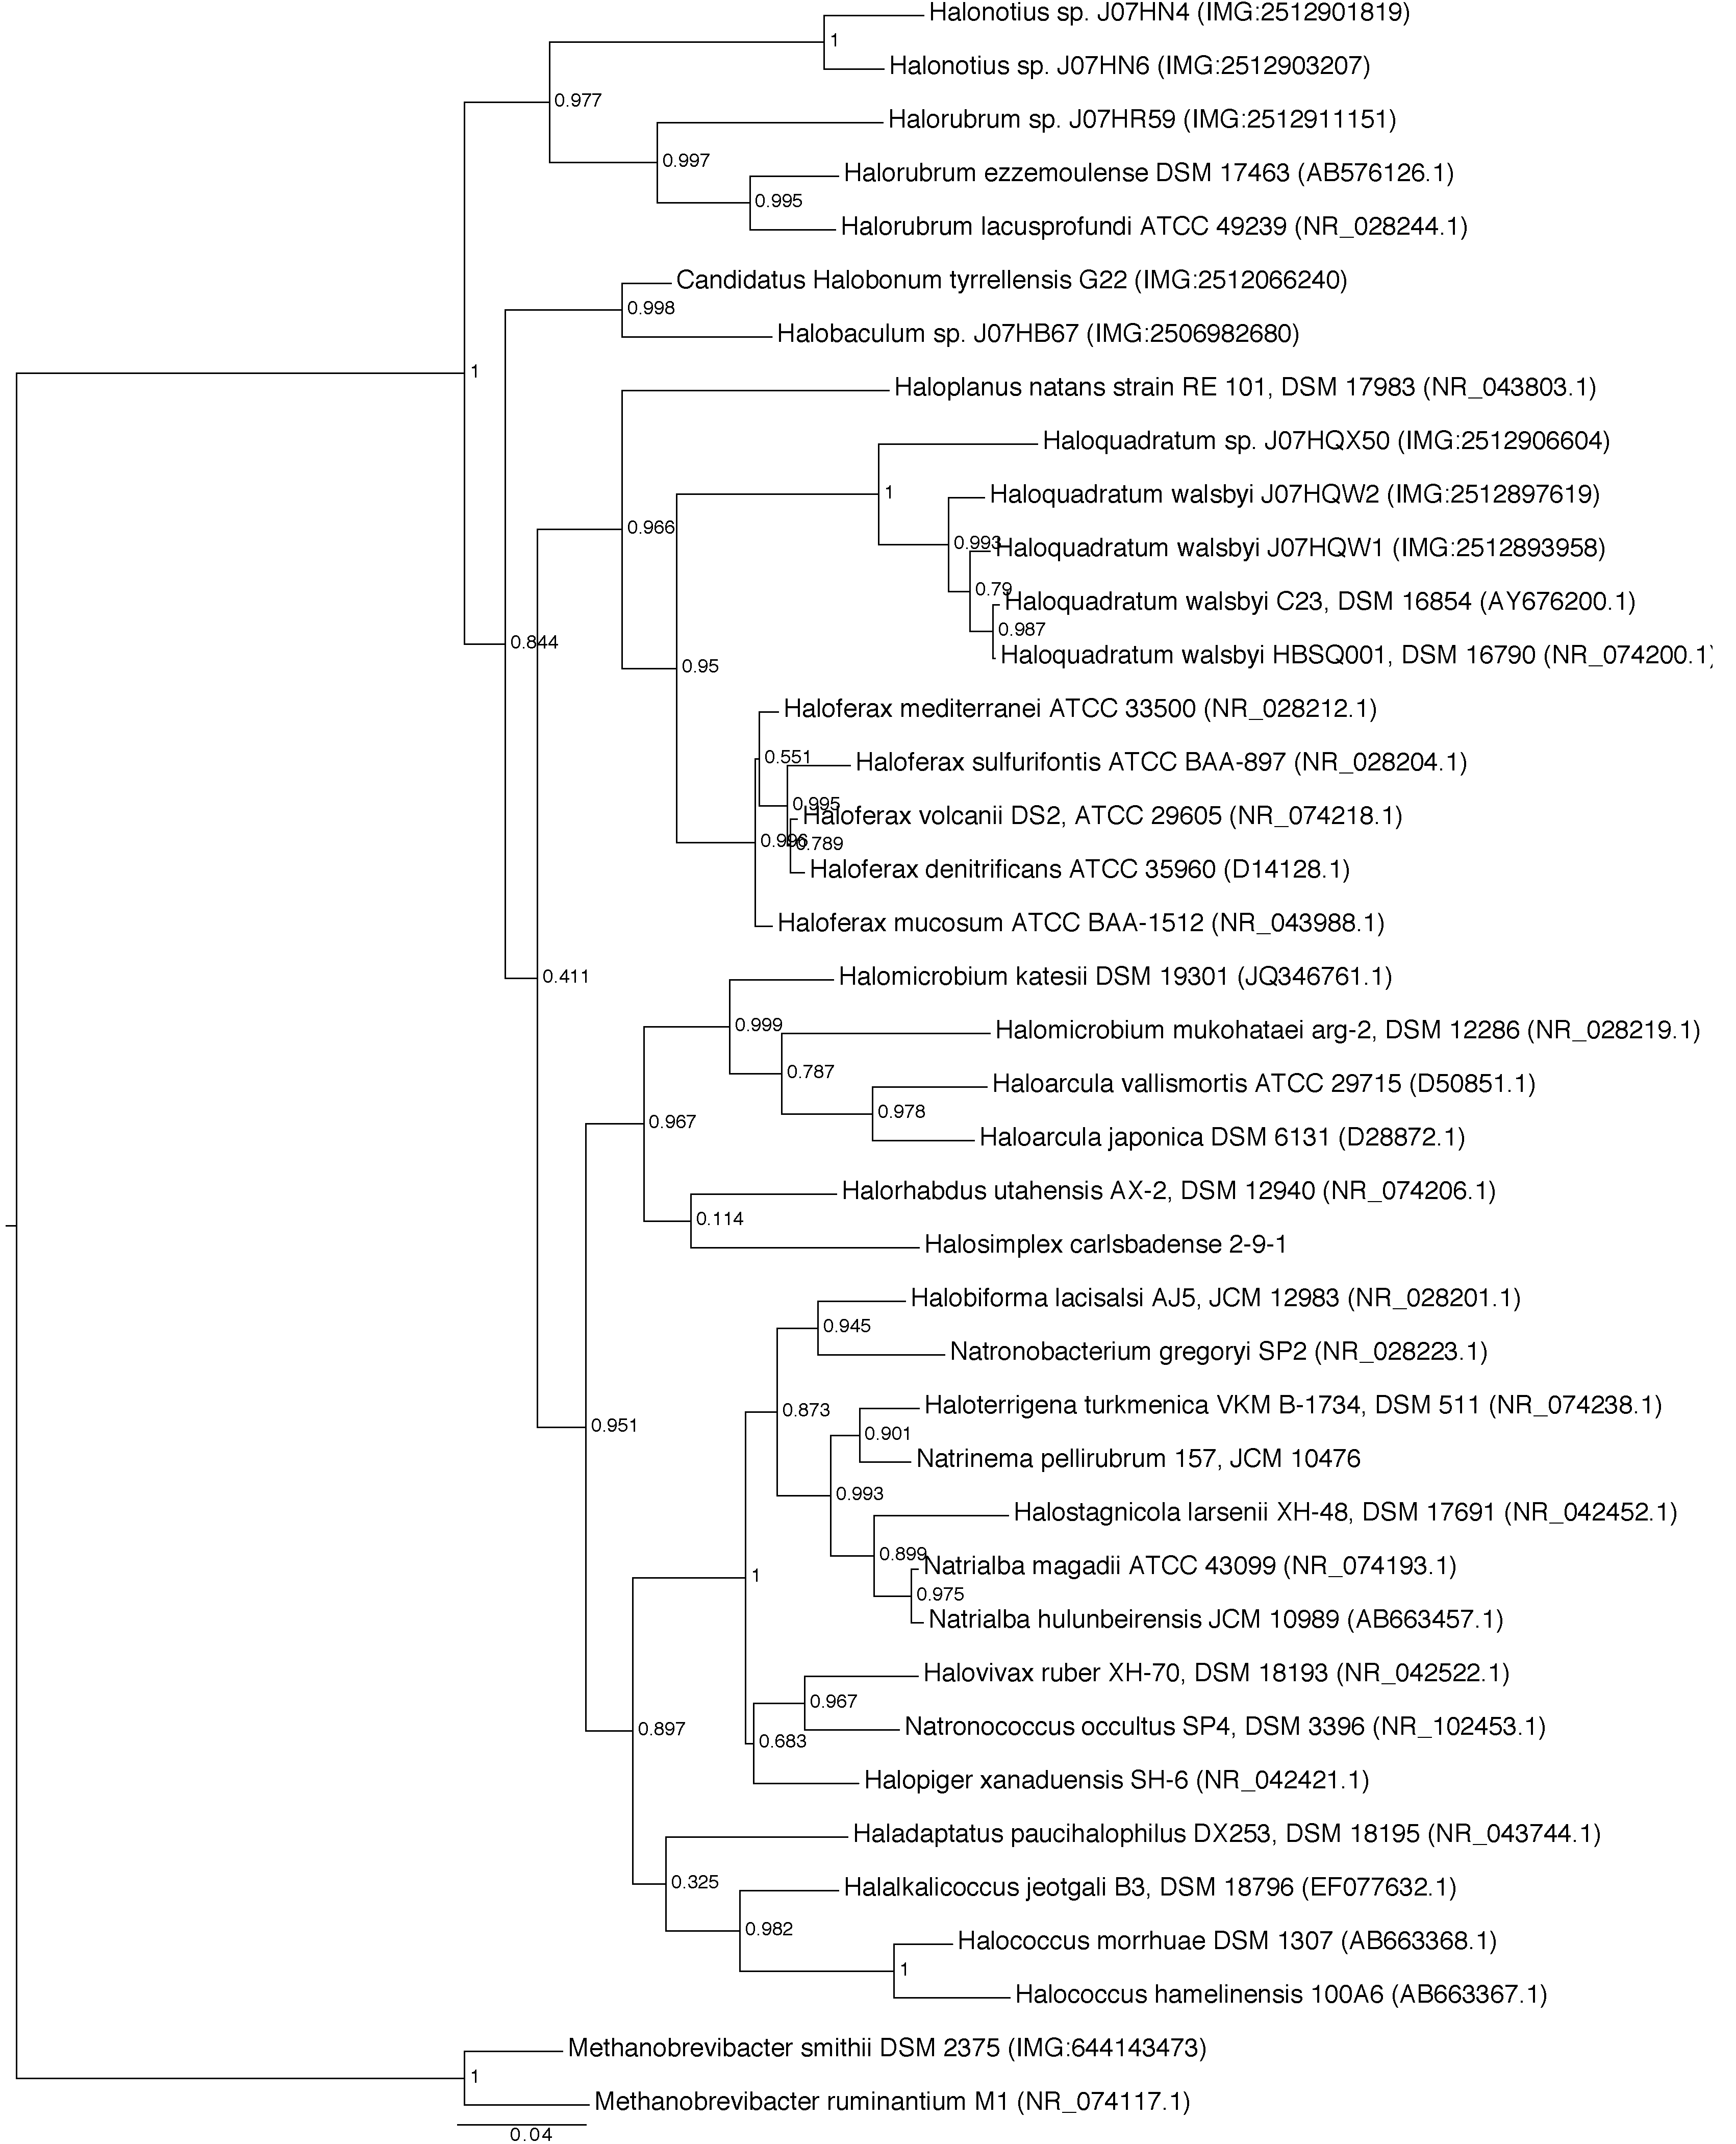
\includegraphics[width=\textwidth]{Chapter1/Figures/HaloG22_16S_v2-2.pdf}
	\caption{Phylogenetic tree of \textit{Candidatus} Halobonum tyrrellensis G22 and related microorganisms, based on 16S rRNA sequences.}
	\label{G22_16Stree}
\end{figure}

%FIGURE, G22, PHYLOPHLA TREE
\begin{figure}[!htbp]
	\centering
	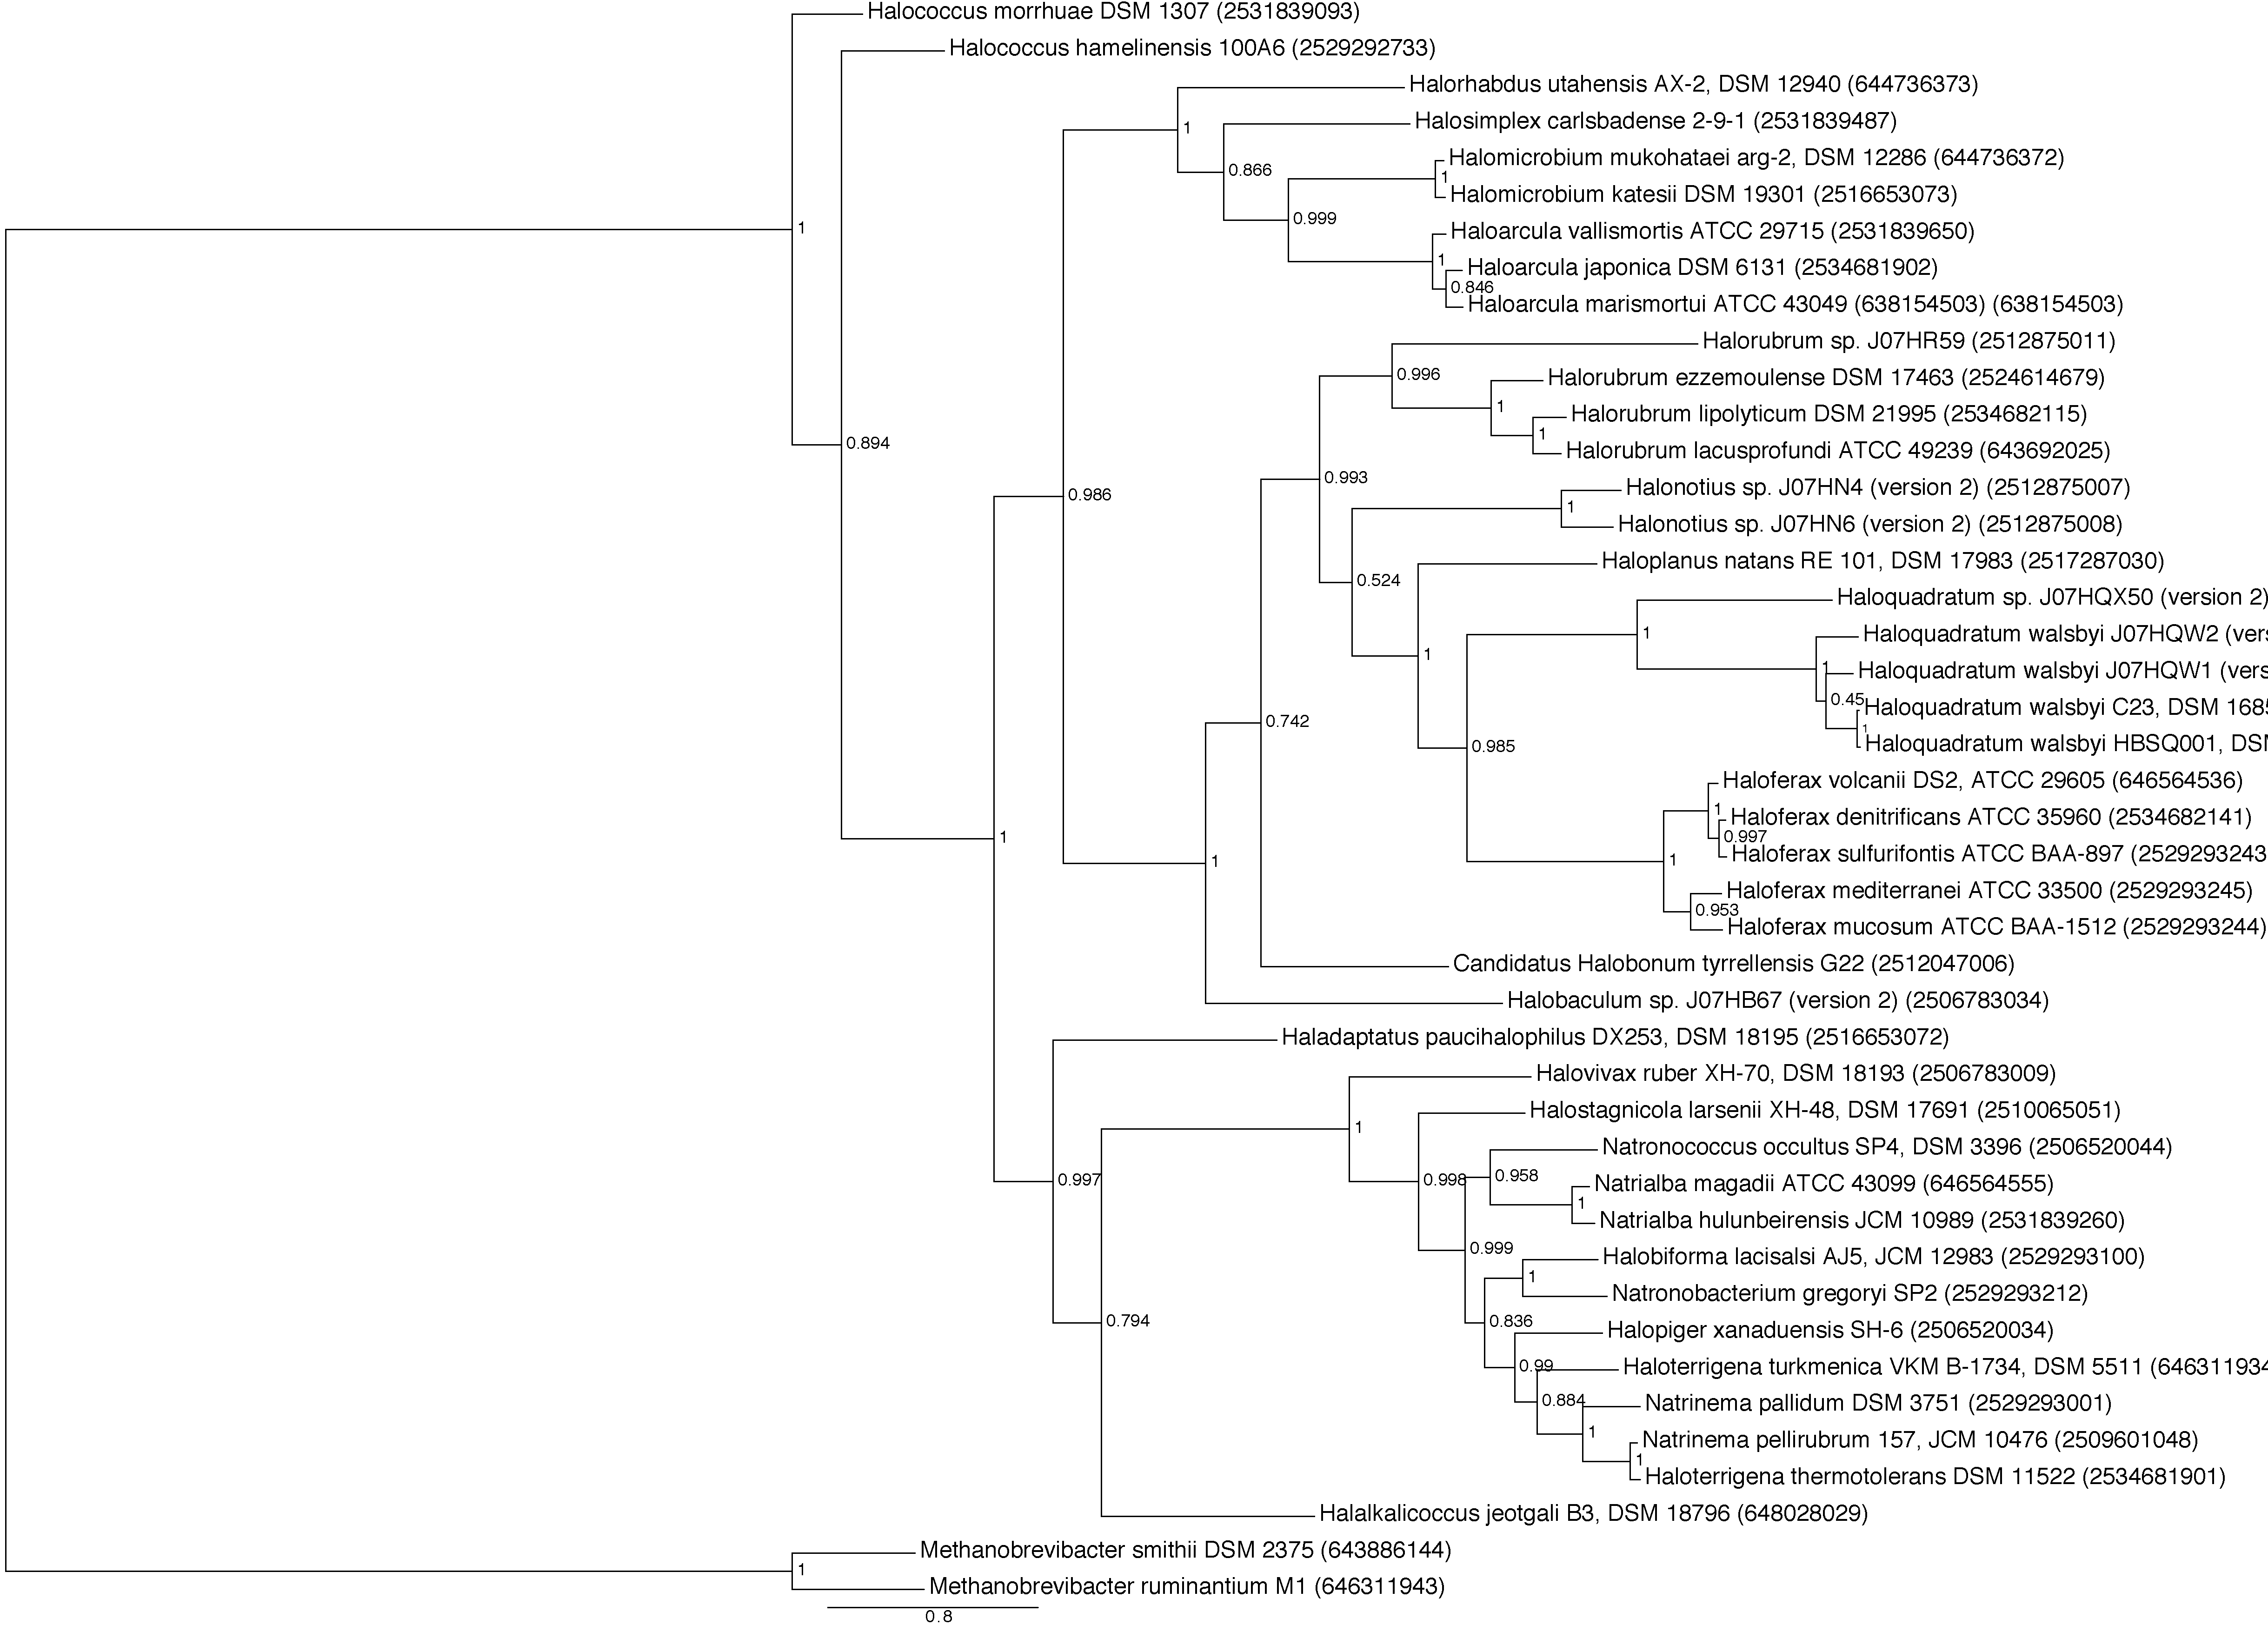
\includegraphics[width=\textwidth]{Chapter1/Figures/HaloG22_v6.pdf}
	\caption{Phylogenetic tree of \textit{Candidatus} Halobonum tyrrellensis G22 and related microorganisms, based on phylogenetic marker sequences implemented in the Phylophlan software \cite{Segata:2013hb}}
	\label{G22_PhyloPhlanTree}
\end{figure}

%FIGURE IONIC COMPOSITION
\begin{figure}[!htbp]
	\centering
	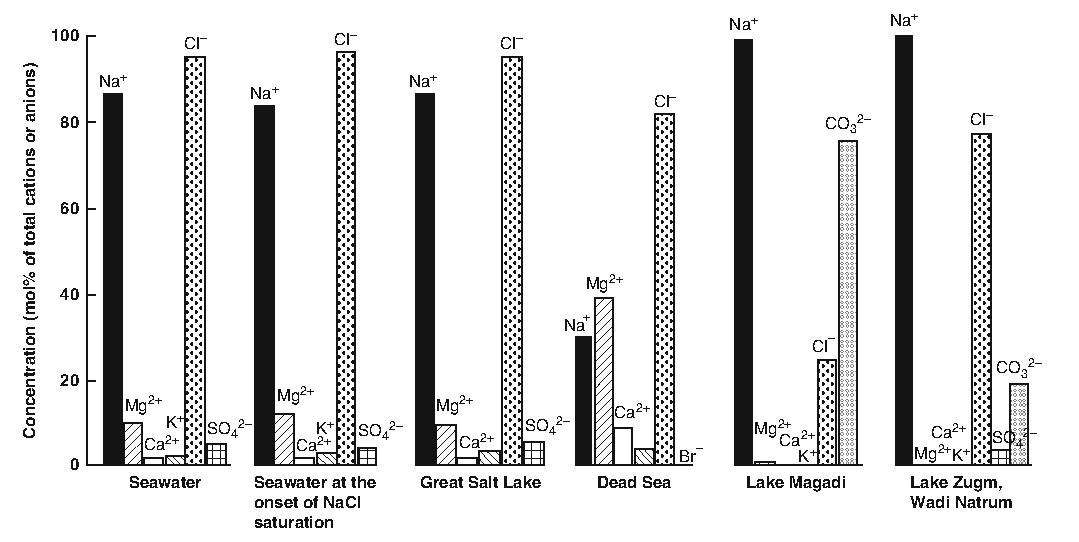
\includegraphics[width=\textwidth]{Chapter1/Figures/IonicComposition.pdf}
	\caption{Ionic composition of several aquatic systems. Figure from Oren, 2013. \cite{Oren:2013bc}}
	\label{IonicComposition}
\end{figure}

%FIGURE IONIC COMPOSITION
\begin{figure}[!htbp]
	\centering
	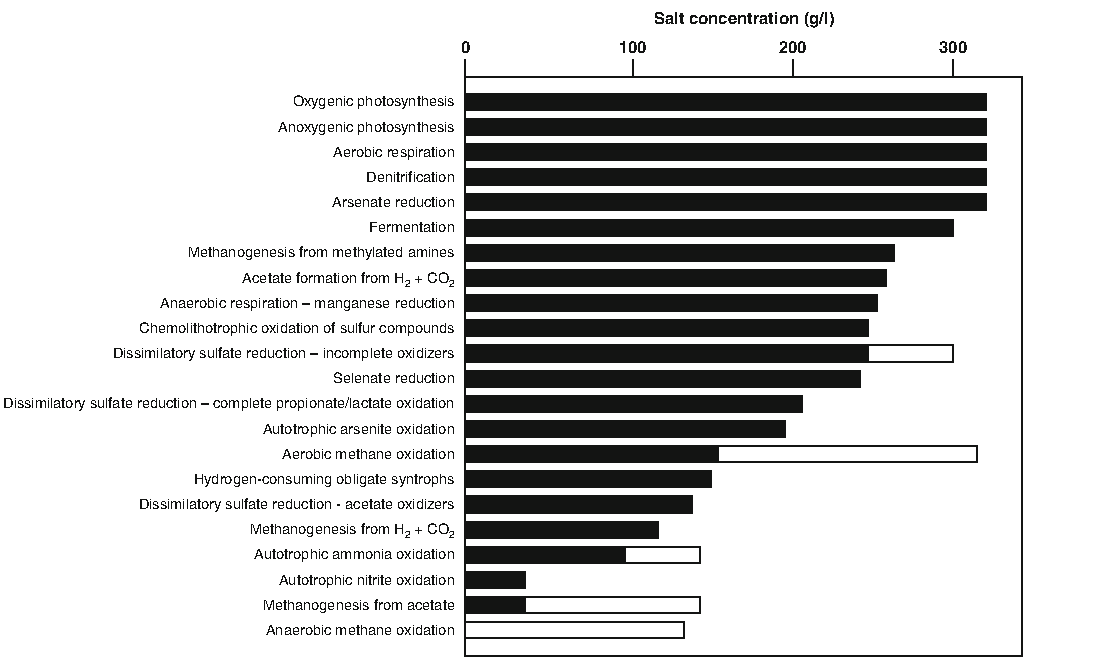
\includegraphics[width=\textwidth]{Chapter1/Figures/HaloMetabolism.pdf}
	\caption{Salt concentration limits for some microbial metabolic processes. Black bars indicate information based on laboratory studies, while white bars indicate activities measured in natural microbial communities. Figure from Oren, 2013 \cite{Oren:2013bc}.}
	\label{HaloMetabolis}
\end{figure}


%TABLE, ARCHAEA DIVERSITY
\begin{table}[!htdp]
\caption{Halophilic Archaea, modified from \cite{Ventosa:2012wo} to include the recently discovered \textit{Nanohaloarchaea} \cite{Narasingarao:2012kp}.}
\begin{center}

\resizebox{\textwidth}{!}{%
\begin{tabularx}{\textwidth}{p{3cm} p{3cm} X}
\hline
\textbf{Phylum} & \textbf{Class} & \textbf{Genera} \\
\hline
\textit{Euryarchaeota} & \textit{Halobacteria} & \textit{Halobacteria, Haladaptatus, Halalkalicoccus, Halarchaeum, Haloarcula, Halobaculum, Halobiforma, Halococcus, Haloferax, Halogeometricum, Halogranum, Halomicrobium, Halonotius, Halopelagius, Halopiger, Haloplanus, Haloquadratum, Halorhabdus, Halorubrum, Halorussus, Halosarcina, Halosimplex, Halostagnicola, Haloterrigena, Halovivax, Natrialba, Natrinema, Natronoarchaeum, Natronobacterium, Natronococcus, Natronolimnobius, Natronomonas, Natronorubrum, Salarchaeum} \\
\cline{2-3} 
& \textit{Methanomicrobia} & \textit{Methanohalobium, Methanocalculus, Methanohalohilus, Methanosalsum} \\
\hline
\textit{Nanohaloarchaea} &  & \textit{Nanosalina, Nanosalinarum} \\
\end{tabularx}
}

\end{center}
\label{TableArchaea}
\end{table}




%TABLE BACTERIA DIVERSITY
\begin{center}

\begin{longtable}{p{3cm} p{4.5cm} p{5.5cm}}
\label{TableBacteria}\\
\caption{Halophilic Bacteria, modified from \cite{Ventosa:2012wo}.}\\

\hline
\textbf{Phylum} & \textbf{Class} & \textbf{Genera} \\
\hline
\endfirsthead

\multicolumn{3}{c}%
{\tablename\ \thetable\ -- \textit{Continued from previous page}} \\
\hline
\textbf{Phylum} & \textbf{Class} & \textbf{Genera} \\
\hline
\endhead

\hline \multicolumn{3}{r}{\textit{Continued on next page}} \\
\endfoot
\hline
\endlastfoot


\textit{Actinobacteria} & \textit{Actinobacteria} & \textit{Actinopolyspora, Amycolatopsis, Georgenia, Corynebacterium, Haloactinobacterium, Haloactinopolyspora, Haloechinothrix, Haloglycomyces, Nesterenjonia, Nocardiopsis, Haloactinospora, Streptomonospora, Isoptericola, Prauserella, Saccharomonospora, Saccharopolyspora} \\
\hline

\textit{Bacteroidetes} & \textit{Bacteroidia} & \textit{Anaerophaga} \\
\cline{2-3}

& \textit{Flavobacteria} & \textit{Gramella, Psychroflexus} \\
\cline{2-3}
& \textit{Sphingobacteria} & \textit{Salinibacter, Salisaeta} \\
\hline

\textit{Cyanobacteria} & & \textit{Rubidibacter, Prochlorococcus, Halospirulina} \\
\hline

\textit{Firmicutes} & \textit{Bacilli} & \textit{Alkalibacillus, Aquisalibacillus, Bacillus, Filobacillus, Gracilibacillus, Halalkalibacillus, Halolactibacillus, Halobacillus, Jeotgalibacillus, Lentibacillus, Oceanobacillus,Ornithinibacillus, Paraliobacillus, Piscibacillus, Pontibacillus, Salimicrobium, Salinibacillus, Salirhabdus, Salsuginibacillus, Sediminibacillus, Salinicoccus, Tenuibacillus, Thalassobacillus, Virgibacillus} \\
\cline{2-3}
& \textit{Clostridia} & \textit{Acetohalobium, Halanaerobacter, Halanaerobium, Halobacteroides, Halocella, Halonatronum, Halothermothrix, Natranaerobius, Natrionella, Natronovirga, Orenia, Selenihalanaerobacter, Sporohalobacter} \\
\hline

\textit{Proteobacteria} & \textit{Alphaproteobacteria} & \textit{Antarctobacter, Citreimonas, Dichotomicrobium, Fodinicurvata, Hwanghaeicola, Hyphomonas, Jannaschia, Maribaculum, Maribius, Marispirillum, Methylarcula, Oceanibulbus, Oceanicola, Palleronia, Paracoccus, Ponticoccus, Rhodobium, Rhodotalassium, Rhodovibrio, Rhodovulum, Roseicitreum, Roseinatronobacter, Roseisalinus, Roseospira, Roseovarius, Salinihabitans, Salipiger, Sediminimonas, Shimia, Sulfitobacter, Tropicibacter, Woodsholea, Yangia} \\
\cline{2-3}
& \textit{Gammaproteobacteria} & \textit{Aidingimonas, Alcanivorax, Alkalilmnicola, Alteromonas, Aestuariibacter, Aquisalimonas, Arhodomonas, Carnimonas, Chromohalobacter, Cobetia, Ectothiorhodspira, Ectothiorhodosinus, Glaciecola, Gilvimarinus, Haliea, Halochromatium, Halomonas, Halorhodospira, Halospina, Halothiobacillus, Idiomarina, Kushneria, Marichromatium, Marinobacter, Marinobacterium, Melitea, Methylohalomonas, Microbulbifer, Modicisalibacter, Nitrincola, Oleispira, Pseudidiomarina, Pseudoaltermonas, Psychromonas, Pseudomonas, Saccarospirillum, Salicola, Salinicola, Salinisphaera, Salinivibrio, Thioalkalibacter, Thioalkalivibrio, Thiohalobacter, Thiohalorhabdus, Thiohalocapsa, Thiohalomonas, Thiohalophilus, Thiohalospira, Thiomicrospira} \\
\cline{2-3}
& \textit{Deltaproteobacteria} & \textit{Desulfocella, Desulfohalobium, Desulfonatronospira, Desulfosalsimonas, Desulfovermiculus, Desulfovibrio, Desulfurivibrio} \\
\cline{2-3}
& \textit{Epsilonproteobacteria} & \textit{Arcobacter, Sulfurimonas, Sulfurovum} \\
\hline

\textit{Spirochaetes} & \textit{Spirochaetes} & \textit{Spirochaeta} \\
\hline

\textit{Tenericutes} & \textit{Mollicutes} & \textit{Haloplasma} \\
\hline

\textit{Thermotogae} & \textit{Thermotogae} & \textit{Petrotoga} \\

\end{longtable}

\end{center}





\section{Lake Tyrrell, Australia, as a model ecosystem}

Lake Tyrrell, Victoria, Australia, is located in the center of the Murray Basin Plains (Figure \ref{LT_map}), in a region with a semi-arid climate, average rainfall of 300 mm/year, and an evaporation rate of ~2000 mm/year  \cite{Macumber:1992ty}. The lake is considered an acid-hypersaline system, where low-pH, oxygenated, saline, metal-rich groundwater from springs is evapo-concentrated and mixed with near-neutral pH waters, rich in sulfides \cite{Long:1992ie}. The lake shows seasonal salinity variations. During winter, the salt content is approximately  \textgreater 250 g/L; in summer, due to water evaporation, the residual brines reach concentrations \textgreater 330 g/L \cite{Macumber:1992ty}.

Lake Tyrrell has been described and studied in detail in terms of its hydrological and geochemical features  \cite{Long:1992ie,Macumber:1992ty,Jones:2006jn}], making it a great candidate for microbiological characterization. Recent projects have used a diverse array of microbiological techniques to study the microbial diversity of Lake Tyrrell, including Eukaryotes \cite{KarlaBHeidelberg:2013jc}, Archaea and Bacteria \cite{Podell:2013kx,Narasingarao:2012kp,Ugalde:2013hb}, and Viruses \cite{Emerson:2012gh,Emerson:tk}. Future work will combine the metagenomic, proteomic, and available geochemical information to provide a more integrative description of the interactions between microbes, viruses, and the environment. 

In this thesis, we explore the microbial diversity of the Lake Tyrrell ecosystem, based on the data generated through a metagenomic study. In particular, our study highlights how, by assembling metagenomic data, we obtain a more complete picture of the microbial diversity present in the community, and also how we can exploit this information to obtain a broad picture of the phylogenetic and functional diversity, and to explore in detail the genetic diversity of the members of the microbial community.

\textbf{Chapter 2} describes how the assembly of metagenomic datasets allowed the recovery and identification of novel microbial groups that are abundant in the hypersaline waters of Lake Tyrrell, and other hypersaline ecosystems. Using additional metadata, such as size fractionation, sequence nucleotide composition, and phylogenetic binning, two near-complete genomes from a novel Class of Archaea, the \textit{Nanohaloarchaea}, were recovered from the metagenomic samples. . This chapter represents work that has already been published  \cite{Narasingarao:2012kp}. My role, in this study was in the classification of sequences into phylogenetic groups using statistical approaches, such as non-metric multidimensional scaling, and exploring the functional diversity of the two novel genomes.

\textbf{Chapter 3} corresponds to the bioinformatic analysis and description of a novel type of microbial rhodopsin, xenorhodopsin, identified from the genomes of the Nanohaloarchaea.The results convey how this rhodopsin appears to be a new class of microbial rhodopsin based on phylogenetic analysis and on the presence of unique amino acid signatures. This work has already been published \cite{Ugalde:2011fw}, where I was the lead author of the study. 

\textbf{Chapter 4} describes the assembly of several genomes from the Lake Tyrrell metagenome, based on the combination of assembly-based approaches and metadata. These results provide a framework for future analyses of this ecosystem, providing a set of habitat-specific genomes, including phylogenetic, functional, and genetic diversity. This work is already published \cite{Podell:2013kx}. My role in this study was developing the methods for classification of the assembled scaffolds into different phylogenetic groups and developing novel visualization and analysis approaches to compare the functional repertoire of community members.

\textbf{Chapter 5}, leverages the assembled habitat-specific genomes, and describes a bioinformatic approach for the analysis of genetic diversity using metagenomic approaches. Using this framework, a deep-sequencing approach was used to characterize the population composition and genetic heterogeneity of two different temporal samples (Summer and Winter) from the microbial members of the Lake Tyrrell community.

%FIGURE LT MAP
\begin{figure}[!htbp]
	\centering
	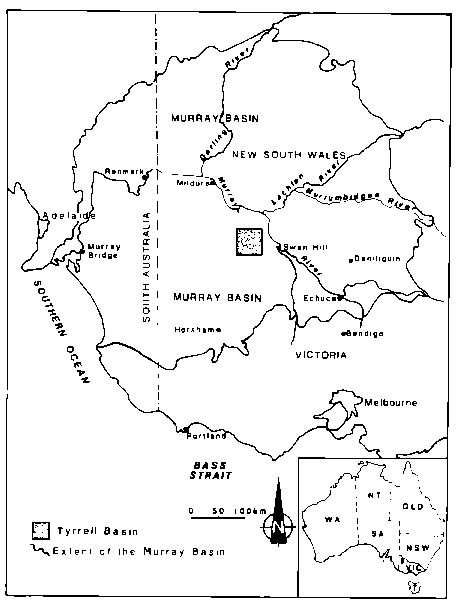
\includegraphics[width=\textwidth]{Chapter1/Figures/LT_Map.pdf}
	\caption{Location of Lake Tyrrell in the southeastern region of Australia. Figure from Macumber, 1992. \cite{Macumber:1992ty}.}
	\label{LT_map}
\end{figure}



%Chapter 2
\chapter{\textit{De novo} metagenomic assembly reveals abundant novel major lineage of Archaea in hypersaline communities}
%Check margins!
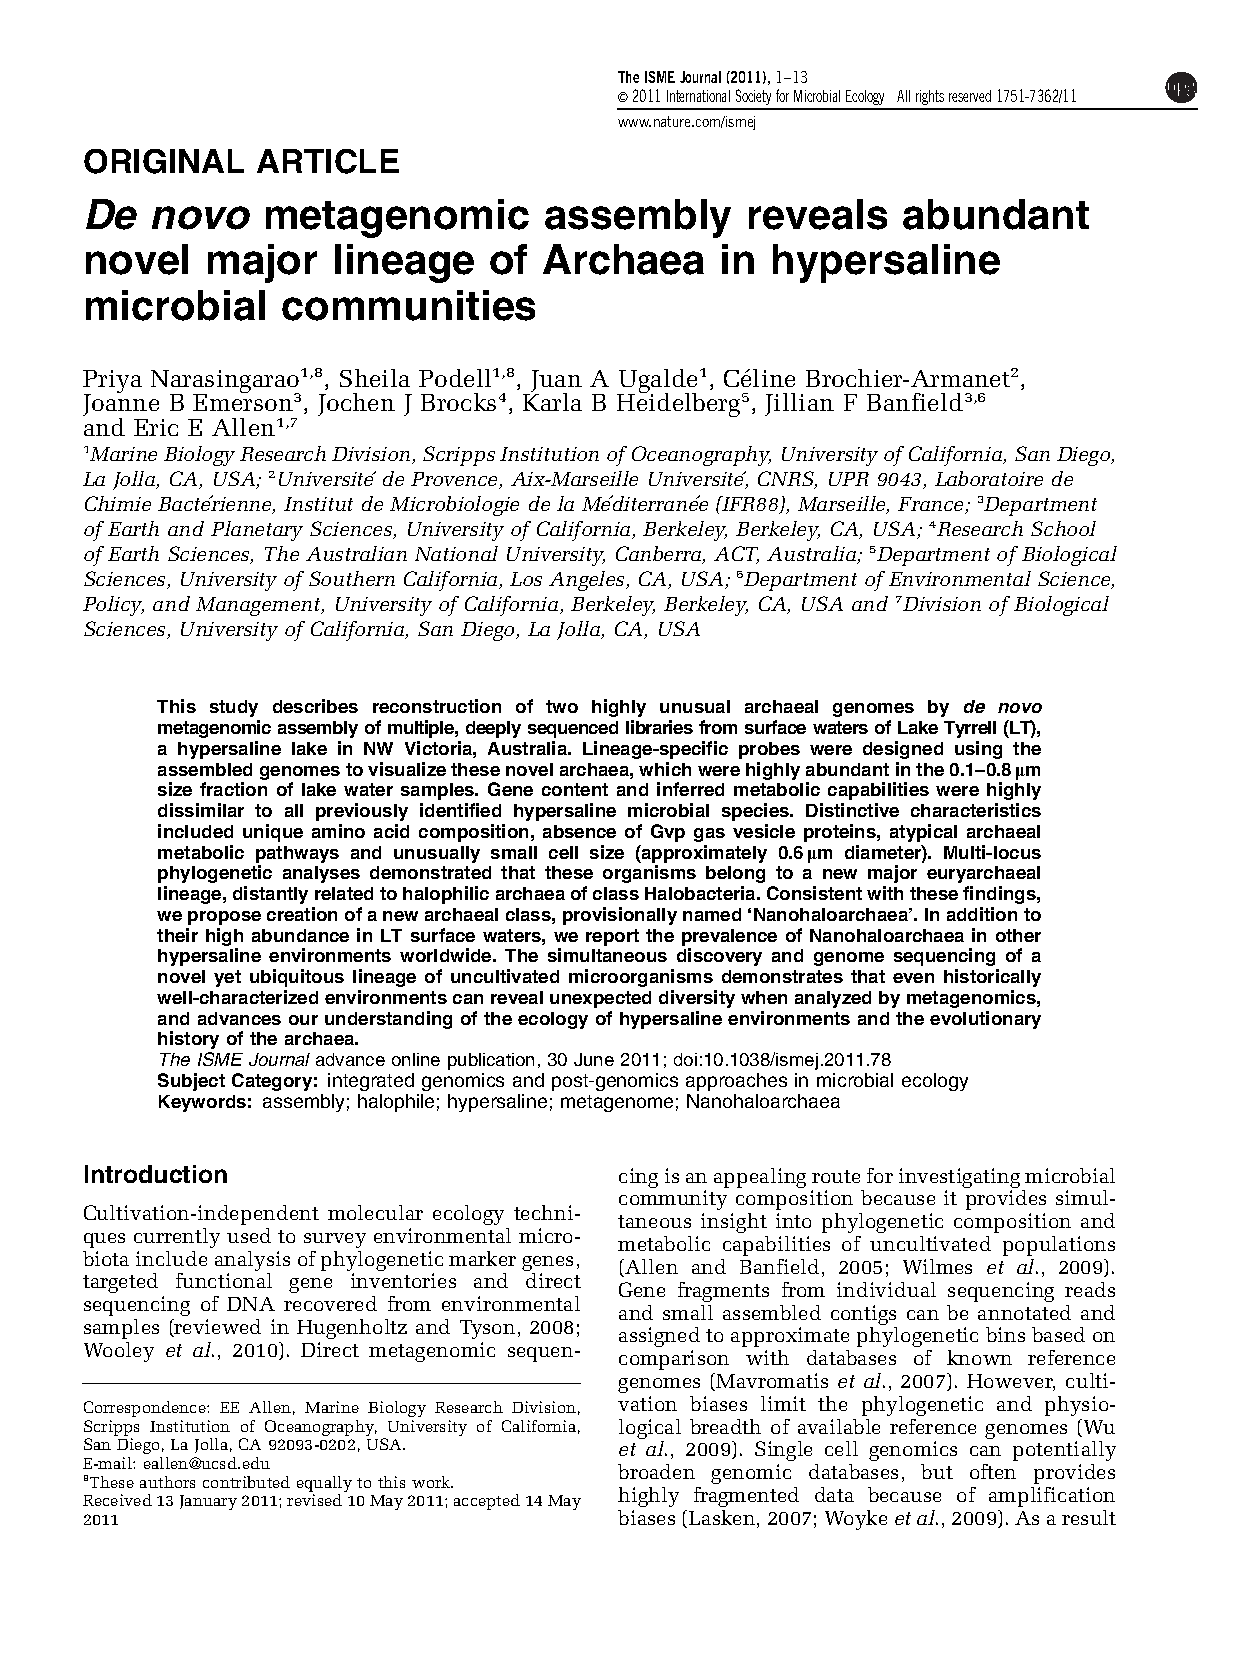
\includepdf[pages={-},fitpaper, scale=0.70,pagecommand={}]{PDFs/Narasingarao2012.pdf}
Chapter 2 is a full reprint of: De novo metagenomic assembly reveals abundant novel major lineage of Archaea in hypersaline communnities. P. Narasingarao, S. Podell, J.A. Ugalde, C. Brochier-Armanet, J.B. Emerson, J.J. Brocks, K.B. Heidelberg, J.F. Banfield and E.E. Allen. \textit{ISME Journal}, \textbf{6},81-93. 2012 (doi: 10.1038/ismej.2011.78), with permission from all coauthors.


%Chapter 3
\chapter{Xenorhodopsins, an enigmatic new class of microbial rhodopsins horizontally transferred between Archaea and Bacteria}
%Check margins!
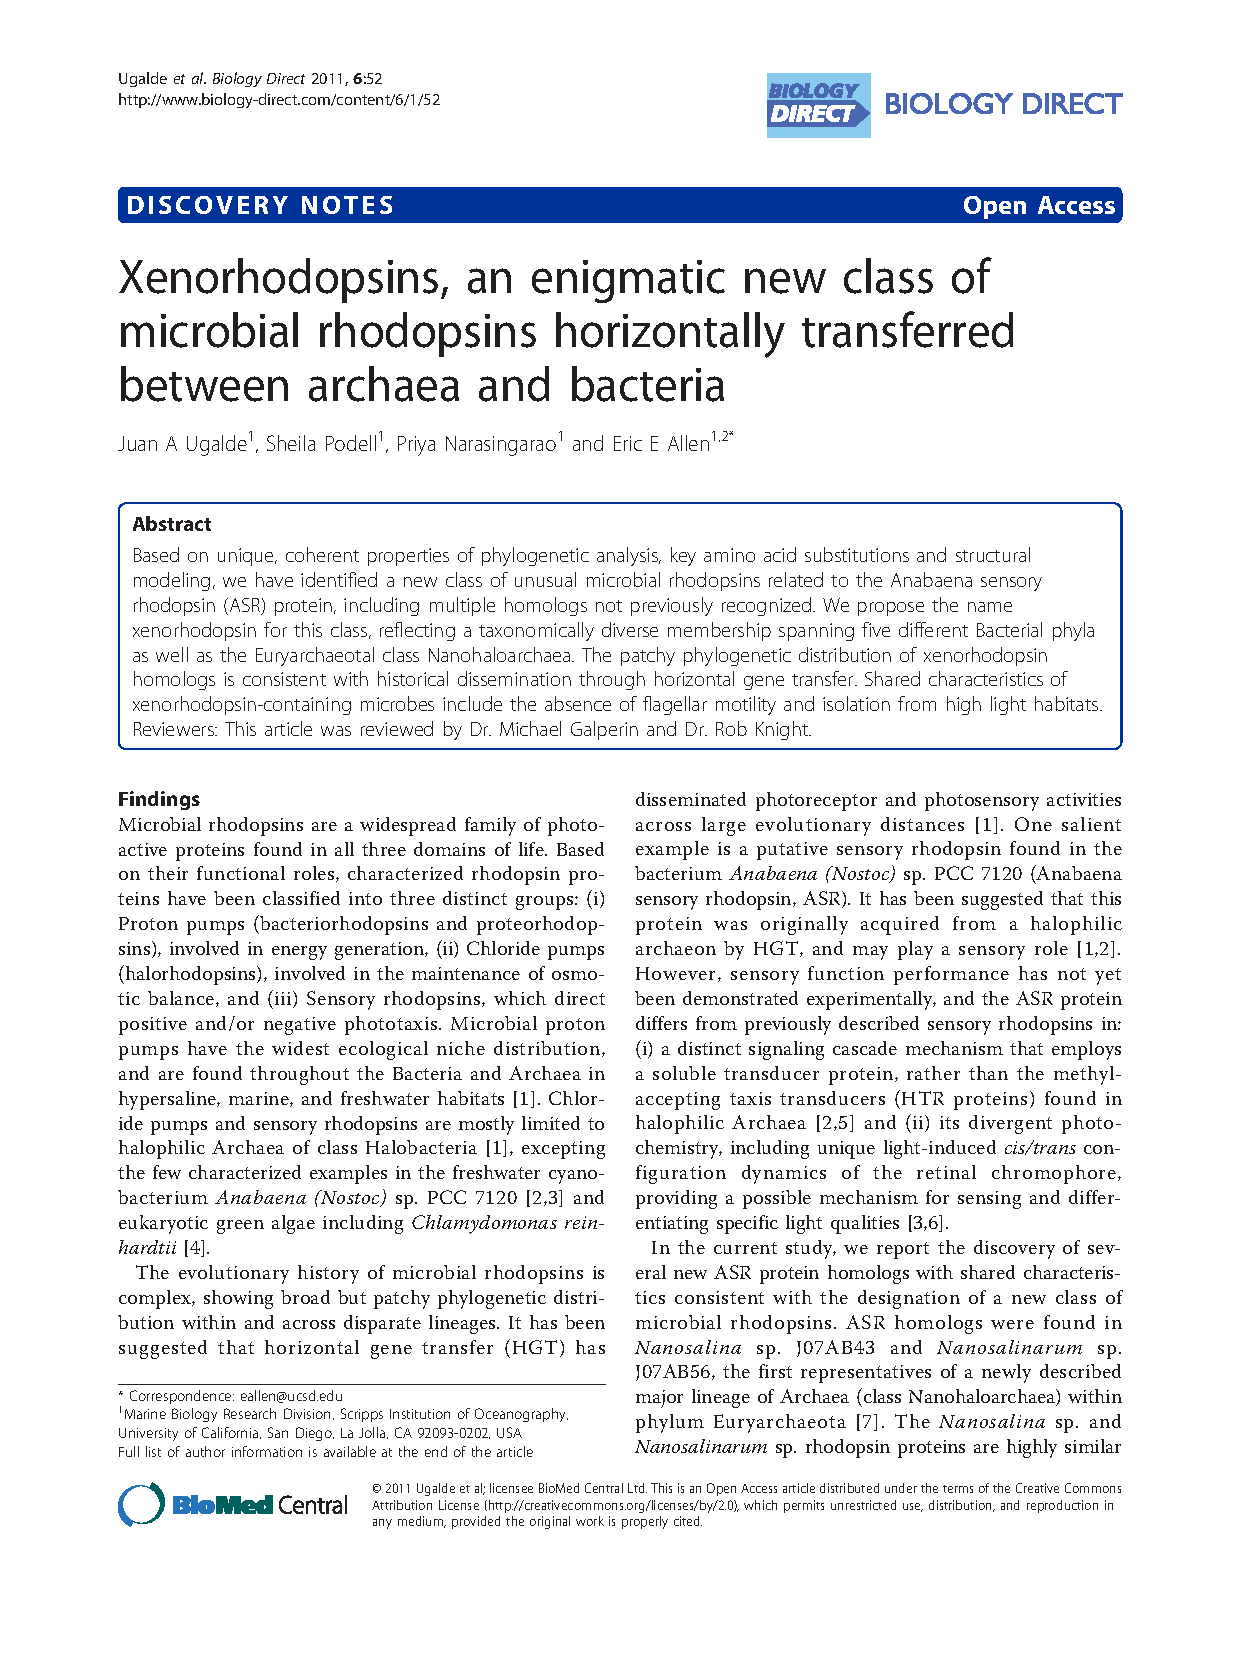
\includepdf[pages={-},fitpaper=true, scale=0.70,pagecommand={}]{PDFs/Ugalde2011.pdf}
Chapter 3 is a full reprint of: Xenorhodopsins, an enigmatic new class of microbial rhodopsins horizontally transferred between archaea and bacteria. J.A. Ugalde, S. Podell, P. Narasingarao and E.E. Allen. \textit{Biology Direct}, \textbf{6},52. 2011 (doi: 10.1186/1745-6150-6-52), with permission from all coauthors.


%Chapter 4
\chapter{Assembly-driven community genomics of a hypersaline microbial ecosystem}
%Check margins!
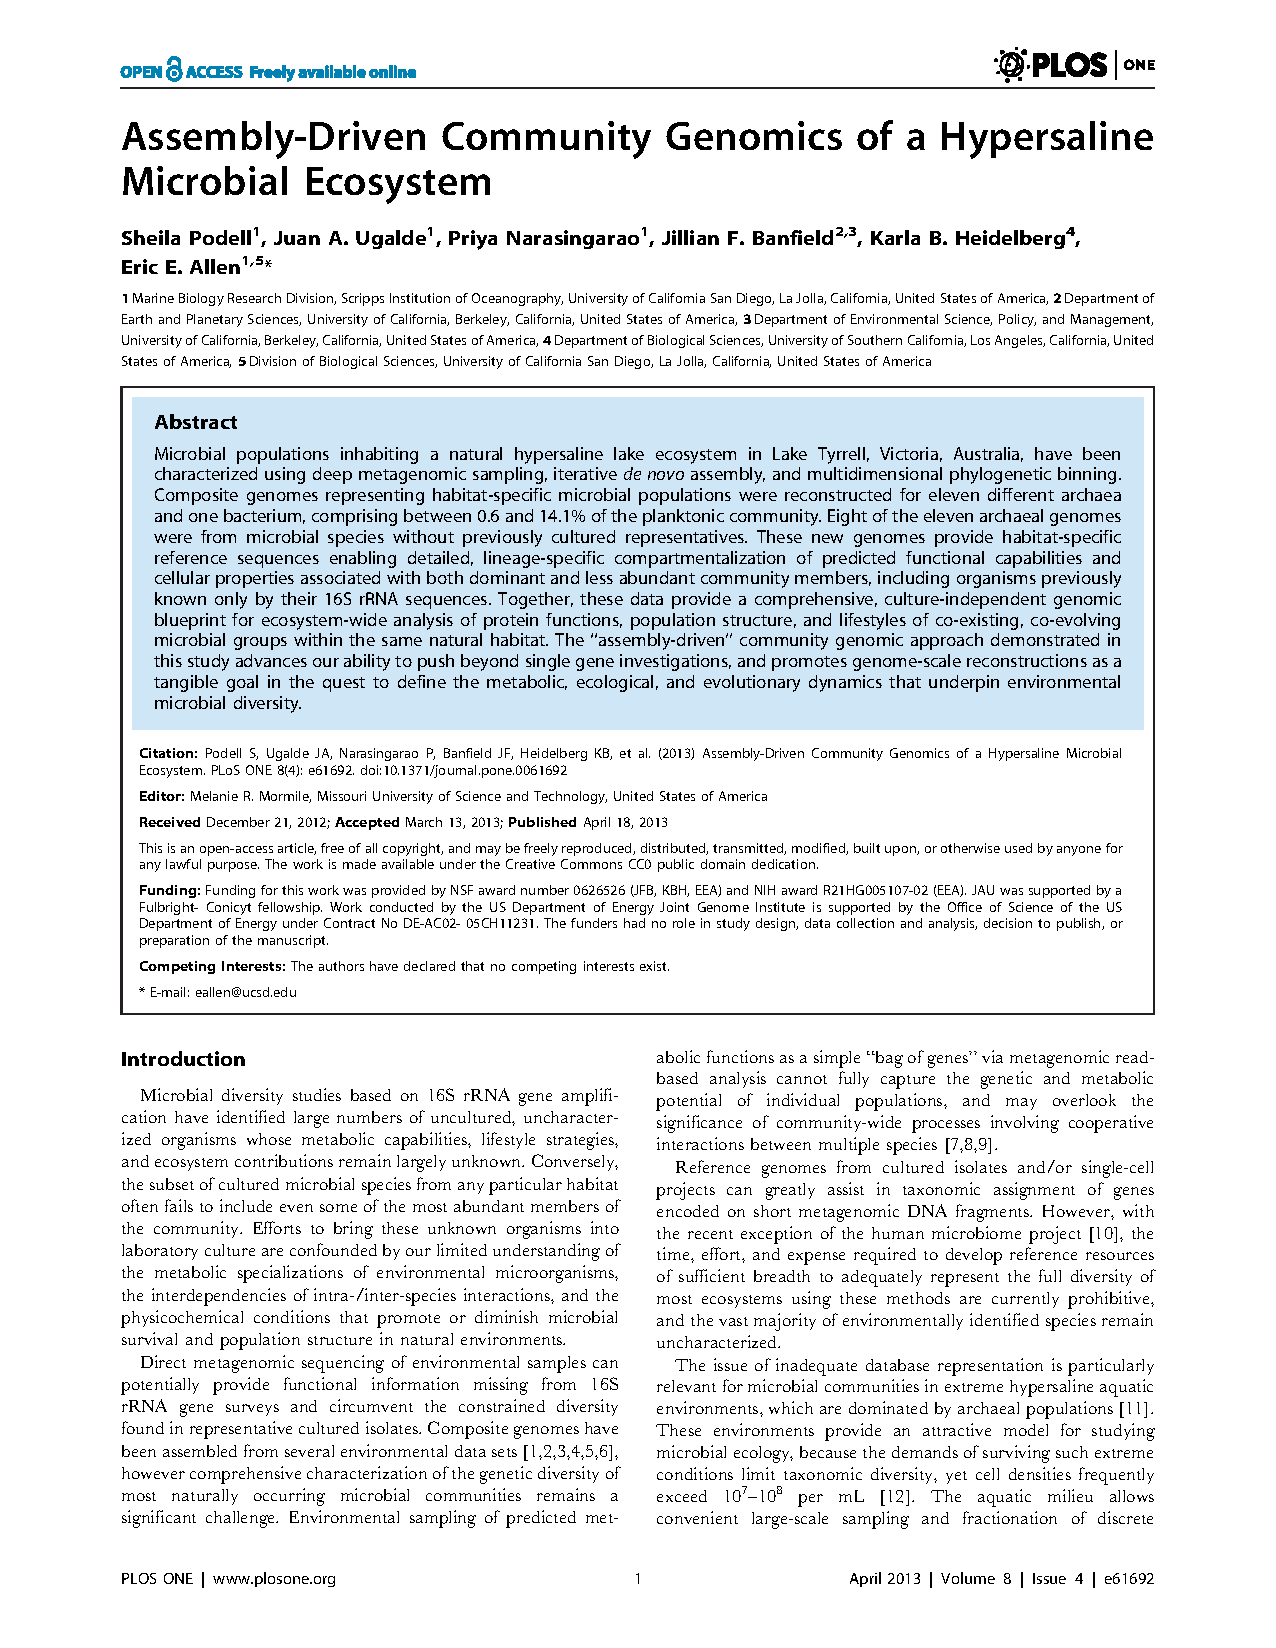
\includepdf[pages={-},fitpaper=true,scale=0.70,pagecommand={}]{PDFs/Podell2013.pdf}
Chapter 4 is a full reprint of: Assembly-driven community genomics of a hypersaline microbial ecosystem. S. Podell, J.A. Ugalde, P. Narasingarao, J.F. Banfield, K.B. Heidelberg and E.E. Allen. \textit{PLoS One}, \textbf{8}4:e61692. 2013 (doi: 10.1371/journal.pone.0061692), with permission from all coauthors.

%Chapter 5
\chapter{Deep-sequencing Approaches to Characterize the Fine-Scale Genetic Variation of the Lake Tyrrell Microbial Ecosystem}

\section{Abstract}

The availability of habitat-specific genomes allows for a comprehensive characterization of the fine-scale genetic diversity that is present in a microbial community. In this chapter, the genetic diversity of the genomes for the Lake Tyrrell microbial community was studied using deeply sequenced metagenomic datasets.

Illumina metagenomic datasets were generated for four samples from the surface waters of Lake Tyrrell collected at different time points (January 23 \& 25 and August 7 \& 9, 2007). Reads were analyzed using the available reference genomes for this community and used to characterize both the abundance of individual populations and the fine-scale genetic diversity present in the community.

Results reveal that for some of the members of the community, such as \textit{Haloquadratum}-related populations, a comparatively low level of strain diversity with almost no differences in the population composition between samples. For other members, such as the \textit{Nanohaloarchaea}, the strain diversity is higher with considerable differences in population composition between samples.

In addition, this analysis allowed the identification of candidate genes under positive selection in some of the populations of the Lake Tyrrell microbial ecosystem. Some of these functions include membrane proteins and secretory systems.

The approach presented in this study represents a broad overview of the fine-scale genetic diversity and generates a foundation for future studies of this community.


\section{Introduction}

The increasing number of microbial genomes sequenced over the last few years has been driven by the higher throughput and lower cost of DNA sequencing technologies. This progress has pushed the field of comparative genomics, allowing for comparisons of the genomes of closely related organisms, up to the strain level  \cite{Fricke:2011gy,Doroghazi:2013gf,Grad:2013tc,Reno:2009bq}, in search of insights into their evolutionary history and environmental adaptation \cite{Reno:2009bq,ZhuofeiXu:2011fp}. This has been a particularly powerful approach in medical microbiology where multiple cultivated strains are available, allowing for a deep coverage of microbial species of medical interest \cite{Feero:2011fr}. Some of this has been replicated in microorganisms isolated from the environment (non-clinical settings), including members of the \textit{Vibrio} genus \cite{Cordero:2012ik} and \textit{Sulfolobus} \cite{Reno:2009bq}.

The development of culture-independent approaches has allowed for removing some of the restrictions of culture-based comparative genomics by allowing us to capture directly the taxonomic, functional, and genetic diversity of the members of microbial community through direct sequencing of environmental DNA \cite{Bragg:2014kv}. A main challenge in the analysis and interpretation of metagenomic data derives due to the genetic complexity of natural microbial communities. In these complex communities, metagenomic approaches often provide only a glimpse of the taxonomic and functional diversity and does not provide enough information to explore the full extent of genetic diversity, particularly at the strain-level.

In the case of low to moderate complexity microbial communities (2-30 dominant microbial species), the use of appropriate sequencing technologies and sampling approaches makes it possible to reconstruct the genomes for dominant community members \cite{Bragg:2014kv}. In reality, these genomes do not represent a single clone, but are a composite of multiple related strains \cite{Podell:2013kx,Allen:2005dg}. This fine-scale genetic variation could have functional relevance for the members of the community, and can reveal information about their evolutionary history and signatures of environmental adaptation \cite{Lo:2007ht,Hemme:2010ds,Palenik:2009kx}.

Several studies have approached the study of microbial communities with the goal of quantifying the level of fine-scale genetic variation present in community members using metagenomic approaches  \cite{Wilmes:2009bn}. These studies can be divided into two categories based on the type of reference data used to quantify genetic heterogeneity. The first category of study obtains metagenomic sequence data from a microbial community and utilizes reference genomes from isolates to quantify the genetic variation present in the microbial community. Examples of this approach include the study of \textit{Synechococcus} coastal populations \cite{Tai:2011jo} and in the human gut microbiome \cite{Schloissnig:2012hx}. The limitation of this type of study is that the reference genomes used are not necessarily derived from the same environment as the metagenomic sample. In addition, it is possible to miss novel and abundant groups, by only focusing on genomes available from isolated species \cite{Podell:2013kx,Herlemann:uy}. ]. A second category of study involves the de novo assembly of metagenomic data and the reconstruction of habitat-specific population genomes from which the genetic heterogeneity present in the community can be quantified. Although this approach provides a more complete and less-biased picture of the genetic diversity, it has largely been limited to communities with low species diversity, such as acid mine drainage \cite{Allen:2007ju} or heavy-metal contaminated sites \cite{Hemme:2010ds}.

Chapters 2 and 4, described studies carried out on the Lake Tyrrell microbial community where the use of assembly-based metagenomics allowed the assembly of one bacterial and 15 archaeal population-level genomes \cite{Narasingarao:2012kp,Podell:2013kx,Podell:2013fp}. These genomes have provided a set of habitat-specific reference genomes that can be used to study fine-scale genetic variability within this community.

Microscale genetic heterogeneity has been previously studied in hypersaline ecosystems via comparative isolate  genomics, such as in the case of \textit{Salinibacter ruber} \cite{PeNtildeA:2010ie}, or using metagenomic approaches \cite{Legault:2006kh,Pasic:2009bo}. In both cases, this has been done using reference genomes from isolates that were not necessarily recovered from the same sampling location where the metagenomic data was recovered. 

This chapter shows the results of a study to quantify the fine-scale genetic diversity that exists in the Lake Tyrrell microbial community. The study combines a deep-sequencing metagenomic approach with the availability of a set of habitat-specific genomes. Two different temporal samples, separated by seven months, were analyzed. The samples were collected in two different seasons, which can provide insights about the stability, both in abundances and in population structure, of this community over time.

%Need to add explanation on what I did here?


\section{Material and Methods}

\subsection{Sample Collection and Sequencing}
Surface water samples from Lake Tyrrell were collected in 2007, during two different seasons, summer (January) and winter (August), with two days of difference in each season (January 23 \& 25, August 7 \& 9). Each water sample was filtered directly onto a Sterivex cartridge (Milipore, Bedford, MA, USA) (\SI{0.22}{\micro\meter}) using a peristaltic pump. For DNA extraction, each Sterivex was processed according to the following protocol:

\begin{itemize}
\item Addition of Proteinase K to a final concentration of 0.5 mg/ml\textsuperscript{-1} and SDS to a final concentration of 1\%.
\item Incubation at 55\textsuperscript{o}C for 25 minutes, followed by incubation at 70\textsuperscript{o}C for 5 minutes.
\item Transfer of the lysate from the Sterivex to a clean Eppendorf tube.
\item Nucleic acid extraction with two steps of phenol-chloroform extraction. 
\end{itemize}

Construction of sequencing libraries for each of the four samples was performed at the UC San Diego IGM Genomics Center. Libraries were multiplexed and sequenced on a single lane of Illumina HiSeq (Illumina, San Diego, CA), using the high-throughput mode, with pair-ended reads of 100 nucleotides in length

The demultiplexed reads were processed using Nesoni 0.117 (\url{http://www.vicbioinformatics.com/software.nesoni.shtml}) to remove adapters, trim low quality positions, and remove low-quality reads from the datasets. For trimming, a minimum quality score of 20 was used, and all reads shorter than 70 nucleotides (after trimming) were removed.

\subsection{Read Mapping}

The trimmed reads were mapped against a set of habitat-specific genomes (Table \ref{GenomeTable} generated by the assembly of metagenomic information of the Lake Tyrrell microbial community \cite{Narasingarao:2012kp,Podell:2013kx,Podell:2013fp}. In addition, an archaeal isolate, \textit{Candidatus} Halobonum tyrrellensis \cite{Ugalde:2013hb}, obtained from samples collected in August of 2007, was included in this set of reference genomes. Each genome is labeled based on their phylogenetic classification on the original work, with the prefix J07 for the genomes representing January samples, and A07 for the genomes that represent August samples. Each metagenomic library (January 23, January 25, August 7 and August 9) was mapped independently to the reference genomes, using Bowtie 2.2.1 \cite{Langmead:2012jh} with the \textit{very-sensitive} alignment option and adjusting the N-ceiling function to (0,0.01) to reduce the number of ambiguous characters present in the alignment. Several tools were used for the analysis of the resulting files, including SAMtools 0.1.19\cite{Li:2009ka}, BEDtools 2.17 \cite{Quinlan:2010km}, and BCFtools 0.2.0 (\url{http://samtools.github.io/bcftools/bcftools.html}).

Coverage plots were generated with custom Python scripts, using the BAM files generated by read mapping.

To determine the differential coverage of each gene in the reference genomes, the RPKM (reads per kilobase per million reads mapped) values were calculated according to the following equation:

\begin{center}
\scalebox{1.2}{
\(
\text{RPKM} = \frac{\text{\textnumero{} of mapped reads to the gene} * \num{e9}}{\text{\textnumero{} of reads mapped in the experiment} * \text{Gene length}}
\)
}
\end{center}

To facilitate the visualization of differences between samples from January and August using the RPKM values, these were normalized using this formula:

\begin{center}
\scalebox{1.2}{
\(
\log_{2}(\frac{\text{January RPKM}}{\text{August RPKM}})
\)
}
\end{center}

A two-tailed Fisher exact test (pvalue $<$ 0.05) was used to determine which genes had differential recruitment of reads between the two seasons (January and August). 
%A complete list of these genes in each of the genomes can be found here (XXX).

\subsection{Taxonomic Classification of Mapped and Unmapped Reads}

To compare the taxonomic diversity found in the mapped and unmapped reads, both sets were classified using Phylosift 1.0.1 \cite{Darling:2014ej}, with the provided set of marker genes. These markers included all of the January 2007 genomes that were assembled previously from the Lake Tyrrell community \cite{Narasingarao:2012kp,Podell:2013kx} (all the genomes with the prefix J07 in Table \ref{GenomeTable}), but did not include the additional Lake Tyrrell genomes recently assembled from metagenomic samples from the August 2007 community, and described in \cite{Podell:2013fp}.

\subsection{Variation Analysis}

The resulting BAM files with the information for the mapped reads were processed with Picard Tools 1.99 (\url{http://picard.sourceforge.net}), to sort and reorder the mapping information. GATK 2.7.2 (\cite{DePristo:2011fo} was used to realign indel regions found by mapping against the reference genomes. These corrected files were processed using Freebayes v9.9.2-29-g9ed353c \cite{Garrison:2012wb} (ploidy:1, minimum base quality: 20, minimum mapping quality: 30) to obtain a set of high-quality variations. Quantification of the type of variations (e.g. single nucleotide polymorphisms, SNPs) was done using SnpEff \cite{Cingolani:2012cz} and visualized using custom Python scripts. 

To calculate the role of selective pressure in each gene, the ratio of non-synonymous to synonymous polymorphisms was calculated. Commonly this ratio is referred as dN/dS, but in this context we are looking at populations (we are not able to distinguish individual members of the population), so it will be referred as pN/pS \cite{Schloissnig:2012hx}. Calculation of the pN/pS values for each coding sequence were done using custom Python scripts, based on the approach used in Tai \textit{et al.} \cite{Tai:2011jo}. For each gene, the pN/pS value was calculated as:

\begin{center}
\scalebox{1.6}{
\(
\frac{\text{pN}}{\text{pS}} = \frac{\frac{\text{Observed non synonymous mutations}}{\text{Number of non synonymous sites}}}{\frac{\text{Observed synonymous mutations}}{\text{Number of synonymous sites}}}
\)
}
\end{center}

All of the visualizations of these results were done using custom Python scripts. To evaluate the differences in functional classifications, the Cluster of Orthologous Groups \cite{Tatusov:2003fk} annotation was used. The comparisons of abundance were done using an odds ratio test:

\begin{center}
\scalebox{1.6}{
\(
\frac{\frac{\text{\textnumero{} of proteins under selection in category X}}{\text{\textnumero{} of proteins not under selection in category X}}}{\frac{\text{Total \textnumero{} of proteins under selection, minus category X}}{\text{Total \textnumero{} of proteins not under selection, minus category X}}}
\)
}
\end{center}

Statistical significance was evaluated using the 2X2 contingency table with a one-tailed Fisher exact test (pvalue $<$ 0.05).


\subsection{Statistical and Computer analysis}

All the analyses were carried out on a large cluster instance (c3.8xlarge: 32 Intel Xeon E5-2680 v2 cores, 60 Gb RAM) using the Elastic Cloud Computing (EC2) infrastructure from Amazon Web Services (AWS). Plotting and calculations were carried out using Python scripts, with the standard packages and the Biopython \cite{Cock:2009hj}, Numpy \cite{Oliphant:2007ud}, Pandas \cite{mckinney-proc-scipy-2010}, PyCogent \cite{Knight:2007gp} and Matplotlib \cite{Hunter:2007ih} libraries. All statistical analyses were carried out using Python scripts and the Scipy libraries \cite{Oliphant:2007ud}. 

%IPython notebooks \cite{Perez:2007wf} and scripts are available on a repository on Github (XXX).


\begin{table}[!htdp]
\small
\caption{List of the Lake Tyrrell habitat-specific genomes used for read mapping}
\begin{center}
\resizebox{\textwidth}{!}{%
\begin{tabularx}{\textwidth}{L{5cm}R{2cm}R{1.4cm}p{2cm}p{1cm}}
\hline
\textbf{Genome name (abbrv)} & \textbf{Length} & \textbf{G+C pct} & \textbf{\textnumero{} scaffolds} & \textbf{Reference} \\
\hline
\textit{Haloquadratum walsbyi} J0HQW1 & 3,549,539 & 47 & 1 & \cite{Podell:2013kx} \\
\textit{Haloquadratum walsbyi} J0HQW2 & 3,475,501 & 49 & 1 & \cite{Podell:2013kx} \\
\textit{Haloquadratum} sp. J07HQX50 & 3,019,909 & 50 & 2 & \cite{Podell:2013kx} \\
\textit{Nanosalinarum} sp. J07AB56 & 1,215,802 & 56 & 3 & \cite{Narasingarao:2012kp} \\
\textit{Nanosalinarum} sp. J07AB43 & 1,277,157 & 43 & 7 & \cite{Narasingarao:2012kp} \\
\textit{Halonotius} sp. J07HN4 & 2,888,659 & 61 & 2 & \cite{Podell:2013kx} \\
\textit{Halonotius} sp. J07HN6 & 2,529,000 & 63 & 6 & \cite{Podell:2013kx} \\
uncultured archaeon sp. J07HX64 & 2,982,938 & 64 & 1 & \cite{Podell:2013kx} \\
uncultured archaeon sp. J07HX5 & 2,040,945 & 60 & 1 & \cite{Podell:2013kx} \\
\textit{Halobaculum} sp. J07HB67 & 2,649,547 & 67 & 3 & \cite{Podell:2013kx} \\
\textit{Halorubrum} sp. J07HR59 & 2,120,805 & 59 & 7 & \cite{Podell:2013kx} \\
\textit{Salinibacter} sp. J07SB67 & 1,931,021 & 67 & 443 & \cite{Podell:2013kx} \\
\textit{Halorubrum} sp. A07HR60 & 2,876,249 & 59 & 14 & \cite{Podell:2013fp} \\
\textit{Halonotius} sp. A07HN63 & 2,392,686 & 63 & 37 & \cite{Podell:2013fp} \\
\textit{Halorubrum} sp. A07HR67 & 2,890,468 & 67 & 16 & \cite{Podell:2013fp} \\
uncultured archaeon A07HB70 & 2,389,822 & 71 & 15 & \cite{Podell:2013fp} \\
\textit{Candidatus} Halobonum tyrellensis G22 & 3,675,087 & 70 & 72 & \cite{Ugalde:2013hb} \\
\hline

\end{tabularx}
}
\end{center}
\label{GenomeTable}
\end{table}


%%%%%%%%%%
\clearpage
\section{Results and Discussion}

\subsection{Overview of the Illumina datasets}

In all four samples, between 71\% and 74\% of the original reads were retained after trimming and quality filtering (Table \ref{LibSequenceQC}), representing an average of 6.9 billion bases per sample.

Preliminary visualization of the community composition was done by looking at the G+C content of each of the libraries. This allows capturing broader differences in community composition between samples \cite{Podell:2013kx,Ghai:2012fb,Podell:2013fp}. Figure \ref{ReadsGCplot} shows the differences between the four libraries, highlighting the location of the reference genomes that will be used for read mapping and where they were recovered from this same community. The plot shows that the January community (in particular, the sample collected on January 25) is dominated by organisms with a low G+C content compared to the August community. This is similar to previous observations for the Lake Tyrrell microbial community \cite{Podell:2013fp}. The main driver of these differences was suggested to be the ionic composition of the water column, particularly the concentration of magnesium, which is higher in the January samples compared to the August ones (Table \ref{LTchemical}) and where microorganisms such as \textit{Haloquadratum} (J07HQW1, J07HQW2, and J07HQX50) are more abundant in the January sample due to their tolerance to higher concentrations of magnesium \cite{Podell:2013fp}. 

Besides the differences between different months among the samples, we can observe differences within the January libraries with different G+C peaks in the January 23 versus the January 25 sample. In particular, the January 25 sample shows a higher peak at lower G+C, compared to the January 23 sample. Looking back into the chemical measurements done for these samples (Table \ref{LTchemical}) \cite{Podell:2013fp}, we can see that the magnesium concentrations on the January 23 sample are lower compared to January 25. Weather records showed that there was an input of freshwater due to a storm prior to the sampling on January 23 \cite{Podell:2013fp}, which suggests an effect on the overall concentrations of dissolved salts, including magnesium. After two days, mainly due to water evaporation, the concentration of dissolved salts in the water column increased, which could explain the difference in the G+C plots and thus the changes in population abundances between the different samples.


%Table, Summary libraries
\begin{table}[hbt]
  \caption{Summary of the total reads before and after trimming, for each of the four Illumina HiSeq libraries.}
  \begin{tabularx}{\textwidth}{L{2.2cm}R{2cm}R{3cm}R{3.2cm}R{2cm}}
  \hline
    \textbf{Library name} & \textbf{Total reads} & \textbf{Read-pairs after QC} & \textbf{Unpaired reads after QC} & \textbf{Total bases (Mb)} \\
    \hline 
    \textit{January 23} & 49,963,357 & 37,016,243 & 7,679,004 & 7,978.18\\
    \textit{January 25} & 39,400,015 & 29,444,267 & 5,894,815 & 6,333.12 \\
    \textit{August 7} & 46,472,319 & 33,485,834 & 7,659,231 & 7,266.38 \\
    \textit{August 9} & 40,256,946 & 28,843,346 & 6,812,171 & 6,276.12 \\
  \end{tabularx}
  \label{LibSequenceQC}
\end{table}
%END

%Figure GC plot
\begin{figure}[!hbtp]
  \centering
  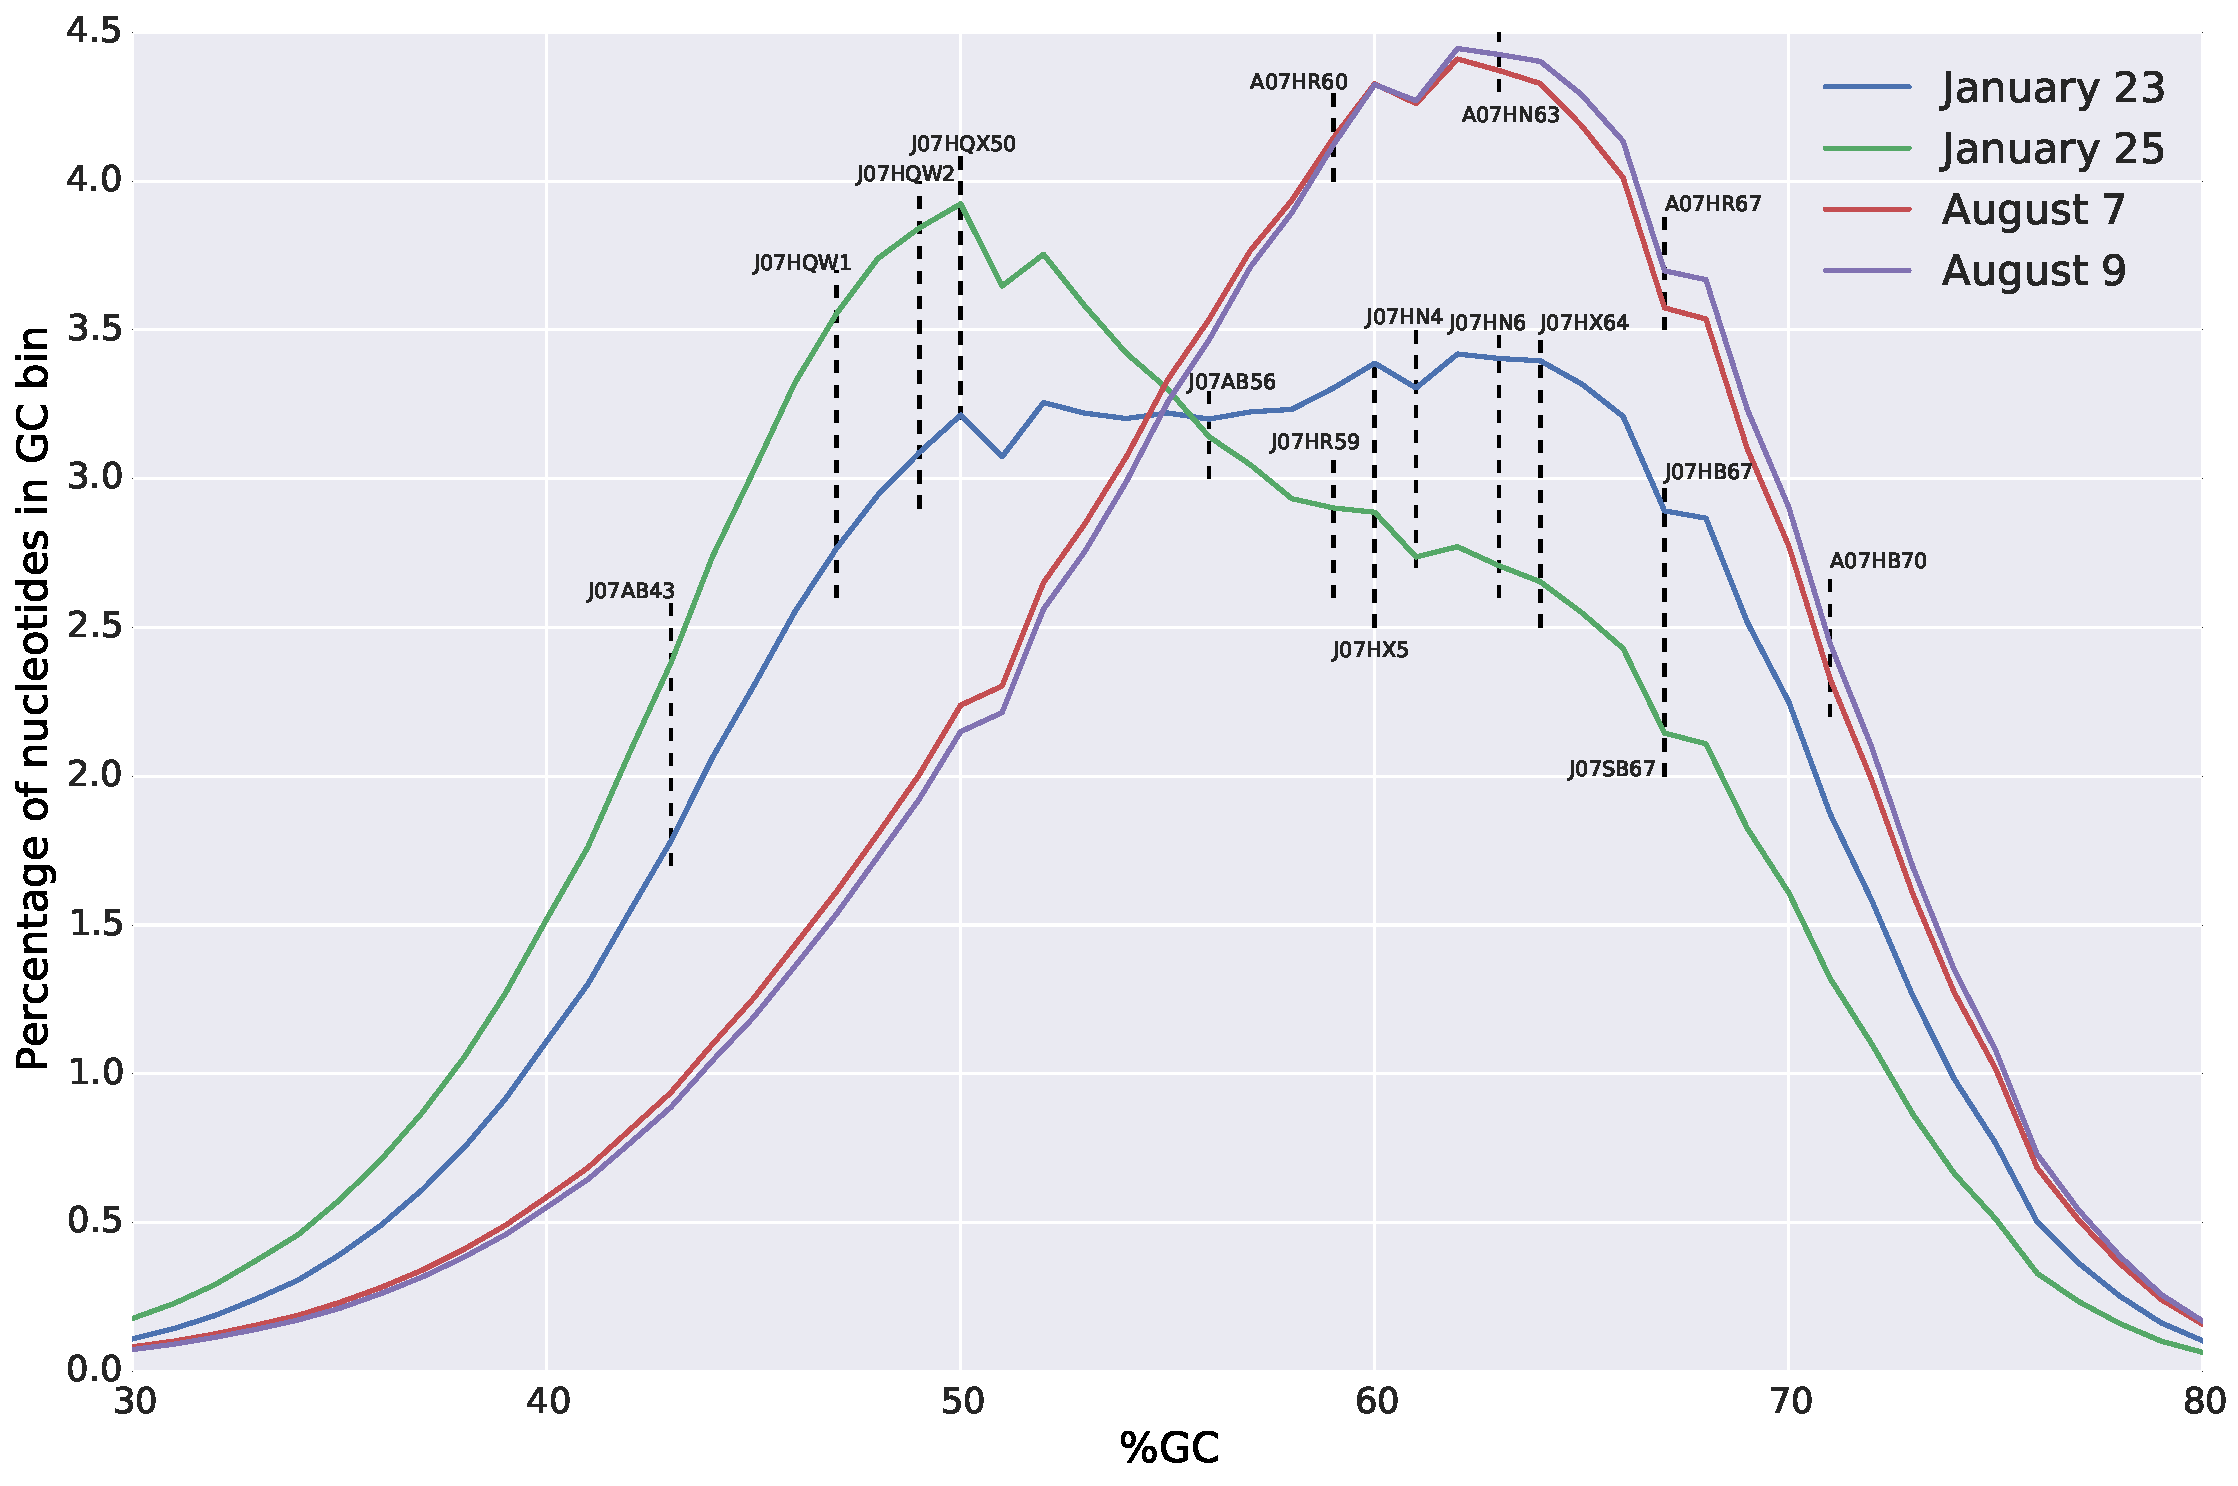
\includegraphics[width=\textwidth]{Chapter5/Figures/GC_content_HiSeqLibs.pdf}
  \caption{Percentage of nucleotides versus G+C content in each of the four sequenced libraries, where each G+C bin has a size of 1\%. Dashed lines indicate the position, based on G+C content, for each of the reference genomes isolated from this community, and that will be used for read mapping (Table \ref{GenomeTable})}
  \label{ReadsGCplot}
\end{figure}
%End of figure

%Table on a new page with facing caption
\clearpage
\thispagestyle{facingcaption}
\begin{table}[h]
\captionsetup{labelformat=prev-page}
\caption{\textbf{Table \ref{LTchemical}:} Physical and chemical composition of the Lake Tyrrell water samples. Concentrations are given in units of \si{\milli\mole\per\liter}}
\label{LTchemical}
\end{table}
\clearpage

\begin{sidewaystable}[h]
\ContinuedFloat
\captionsetup{labelformat=empty}
\centering

\begin{tabular}{cccccccccc}

\textbf{Sample} & \textbf{Temp \si{\degreeCelsius}} & \textbf{Total ionic strength} & \textbf{Na} & \textbf{K} & \textbf{Mg} & \textbf{Ca} & \textbf{Cl} & \textbf{Cl} & \textbf{SO42} \\
\hline
\textit{Jan 23} & 21.6 & pH & 5,721 & 4,338 & 32 & 298 & 10 & 5,345 & 123.6 \\
\textit{Jan 25} & 27.9 & 7.09 & 5,950 & 4,163 & 43 & 419 & 11 & 5,291 & 170.5 \\
\textit{Aug 6} & 9.9 & 7.00 & 4,403 & 3,724 & 19 & 126 & 15 & 4,298 & 50 \\
\textit{Aug 8} & 11.5 & 7.01 & 4,060 & 3,557 & 18 & 117 & 14 & 3,830 & 47 \\

\end{tabular}
\end{sidewaystable}

%%%%End of table

%END OF SECTION
\clearpage
\subsection{Read Mapping using Habitat-Specific genomes}

All the reads that passed the quality filters were mapped against the set of habitat-specific genomes (Table \ref{GenomeTable}) from the Lake Tyrrell community. The results indicate differences in the number of reads that each genome recruited, both comparing between samples and between genomes (Table \ref{ReadRecruitmentGenome}). 

In the January samples, the genomes that recruited the most number of reads were those associated with \textit{Haloquadratum} (J07HWQ1 and J07HWQ2), which agrees with previous observations regarding the abundance of these organisms in the Lake Tyrrell community \cite{Podell:2013kx}. The raw number of reads does not provide the best criteria to estimate the relative abundance of each genome in the overall dataset as these genomes vary in size. Rather, the depth of coverage for each genome (Table \ref{ReadCoverageGenome}) provides a better metric for these estimations. The overall coverage, shows similar relative abundances compared to previous observations \cite{Podell:2013kx}, but it is important to highlight that the number of mapped reads and the coverage do not necessarily reflect the real abundance of each organism in the community. Given the strict criteria used for mapping, it is likely that many sequences that could be recruited onto individual genomes could be missing. For example, the stringent criteria used could explain the low number of reads and low coverage for the genome of \textit{Candidatus} Halobonum turrellensis (G22). This particular organism is an interesting case because it is the only genome that was obtained from an isolate (cultured from August 2007 samples) \cite{Ugalde:2013hb}, but its abundance in the community appears to be very low compared to the other genomes that were recovered via metagenomic assembly. This is a clear example of the often observed phenomenon where cultured isolates from an environment are not representative of the most abundant members of a microbial community.

We can estimate how stringent the mapping criteria were by looking at the sequence identity of each read compared to the mapped genome and quantifying this for each library and genome (Figure \ref{GenomeReadIdentity}). With the exception of the G22 genome, the majority of reads mapped at a 100\% sequence identity, and it was never lower than 85\% for any of the genomes and libraries. This analysis alone provides an accurate overview of the level of genetic heterogeneity that is present in these populations. For example, for the \textit{Haloquadratum} genomes, the majority of the reads mapped at 95\% sequence identity, while in the case of the \textit{Nanohaloarchaea} genomes, the sequence identity of the recruited reads goes down to 89\%.

%%TABLES AND FIGURES
%Table, reads recruited
\begin{table}[ht!]
  \caption{Total number of recruited reads to each reference genome.}
  \begin{tabularx}{\textwidth}{L{2.2cm}R{2cm}R{3cm}R{3.2cm}R{2cm}}
  \hline
    \textbf{Genome} & \textbf{Jan 23} & \textbf{Jan 25} & \textbf{Aug 07} & \textbf{Aug 09} \\
    \hline
     \textit{J07HWQ1} & 9,712,976 & 10,347,084 & 1,802,421 & 1,385,337 \\
     \textit{J07HWQ2} & 7,311,175 & 9,428,490 & 1,628,137 & 1,301,141 \\
     \textit{J07HQX50} & 922,138 & 1,041,326 & 501,477 & 330,307 \\
     \textit{J07AB56} & 565,197 & 266,831 & 194,445 & 165,278 \\
     \textit{J07AB43} & 760,203 & 486,360 & 63,209 & 64295 \\
     \textit{J07HN4} & 2,149,204 & 2,249,692 & 1,306,287 & 1,089,673 \\
     \textit{J07HN6} & 592,818 & 831,367 & 1,027,472 & 911,341 \\
     \textit{J07HX64} & 4,167,113 & 1,819,023 & 1,202,103 & 1,144,206 \\
     \textit{J07HX5} & 2,106,559 & 1,382,371 & 673,972 & 539,843 \\
     \textit{J07HB67} & 1,124,816 & 1,128,191 & 125,973 & 84,643 \\
     \textit{J07HR59} & 839,856 & 310,496 & 2,105,598 & 1,693,772 \\
     \textit{A07HB70} & 550,429 & 277,030 & 1,970,106 & 1,866,967 \\
     \textit{A07HR67} & 563,043 & 270,602 & 2,166,129 & 1,680,150 \\
     \textit{A07HN63} & 547,808 & 786,856 & 1,126,032 & 1,003,322 \\
     \textit{A07HR60} & 2,126,700 & 758,549 & 5,405,933 & 4,362,857 \\
     \textit{G22} & 62,983 & 39,696 & 72,261 & 66,778 \\
     \textit{J07SB} & 797,957 & 211,306 & 737,471 & 673,630 \\     
  \textit{Unmapped} & 45,344,829 & 31,913,858 & 51,012,461 & 44,849,506 \\
  \end{tabularx}
  \label{ReadRecruitmentGenome}
\end{table}

%Table, reads coverage
\begin{table}[ht!]
  \caption{Genomes coverage (expressed as X-fold) in each of the libraries.}
  \begin{tabularx}{\textwidth}{L{2.2cm}R{2cm}R{3cm}R{3.2cm}R{2cm}}
  \hline
    \textbf{Genome} & \textbf{Jan 23} & \textbf{Jan 25} & \textbf{Aug 07} & \textbf{Aug 09} \\
    \hline
     \textit{J07HWQ1} & 274.9 & 292.7 & 51.0 & 39.2 \\
     \textit{J07HWQ2} & 200.2 & 258.0 & 44.5 & 35.6 \\
     \textit{J07HQX50} & 30 & 33.9 & 16.3 & 10.7 \\
     \textit{J07AB56} & 45.5 & 21.5 & 15.6 & 13.2 \\
     \textit{J07AB43} & 61.2 & 39.1 & 5.1 & 5.2 \\
     \textit{J07HN4} & 72.4 & 75.7 & 44.0 & 36.7 \\
     \textit{J07HN6} & 22.8 & 31.9 & 39.4 & 35.0 \\
     \textit{J07HX64} & 135.5 & 59.1 & 39.1 & 37.2 \\
     \textit{J07HX5} & 100.5 & 65.9 & 32.1 & 25.7 \\
     \textit{J07HB67} & 40.9 & 41.0 & 4.6 & 3.1 \\
     \textit{J07HR59} & 38.6 & 14.2 & 96.7 & 77.7 \\
     \textit{A07HB70} & 22.1 & 11.1 & 79.1 & 74.9 \\
     \textit{A07HR67} & 18.8 & 9.0 & 72.2 & 56.0  \\
     \textit{A07HN63} & 22.2 & 31.9 & 45.7 & 40.7 \\
     \textit{A07HR60} & 72.0 & 25.7 & 183.1 & 147.7 \\
     \textit{G22} & 1.6 & 1.0 & 1.9 & 1.7 \\
     \textit{J07SB} & 40.1 & 10.6 & 37.1 & 33.8 \\     
  \end{tabularx}
  \label{ReadCoverageGenome}
\end{table}


%Figures for this section

%Figure, Genome Identity Plots
\begin{figure}[!hbtp]
  \centering
  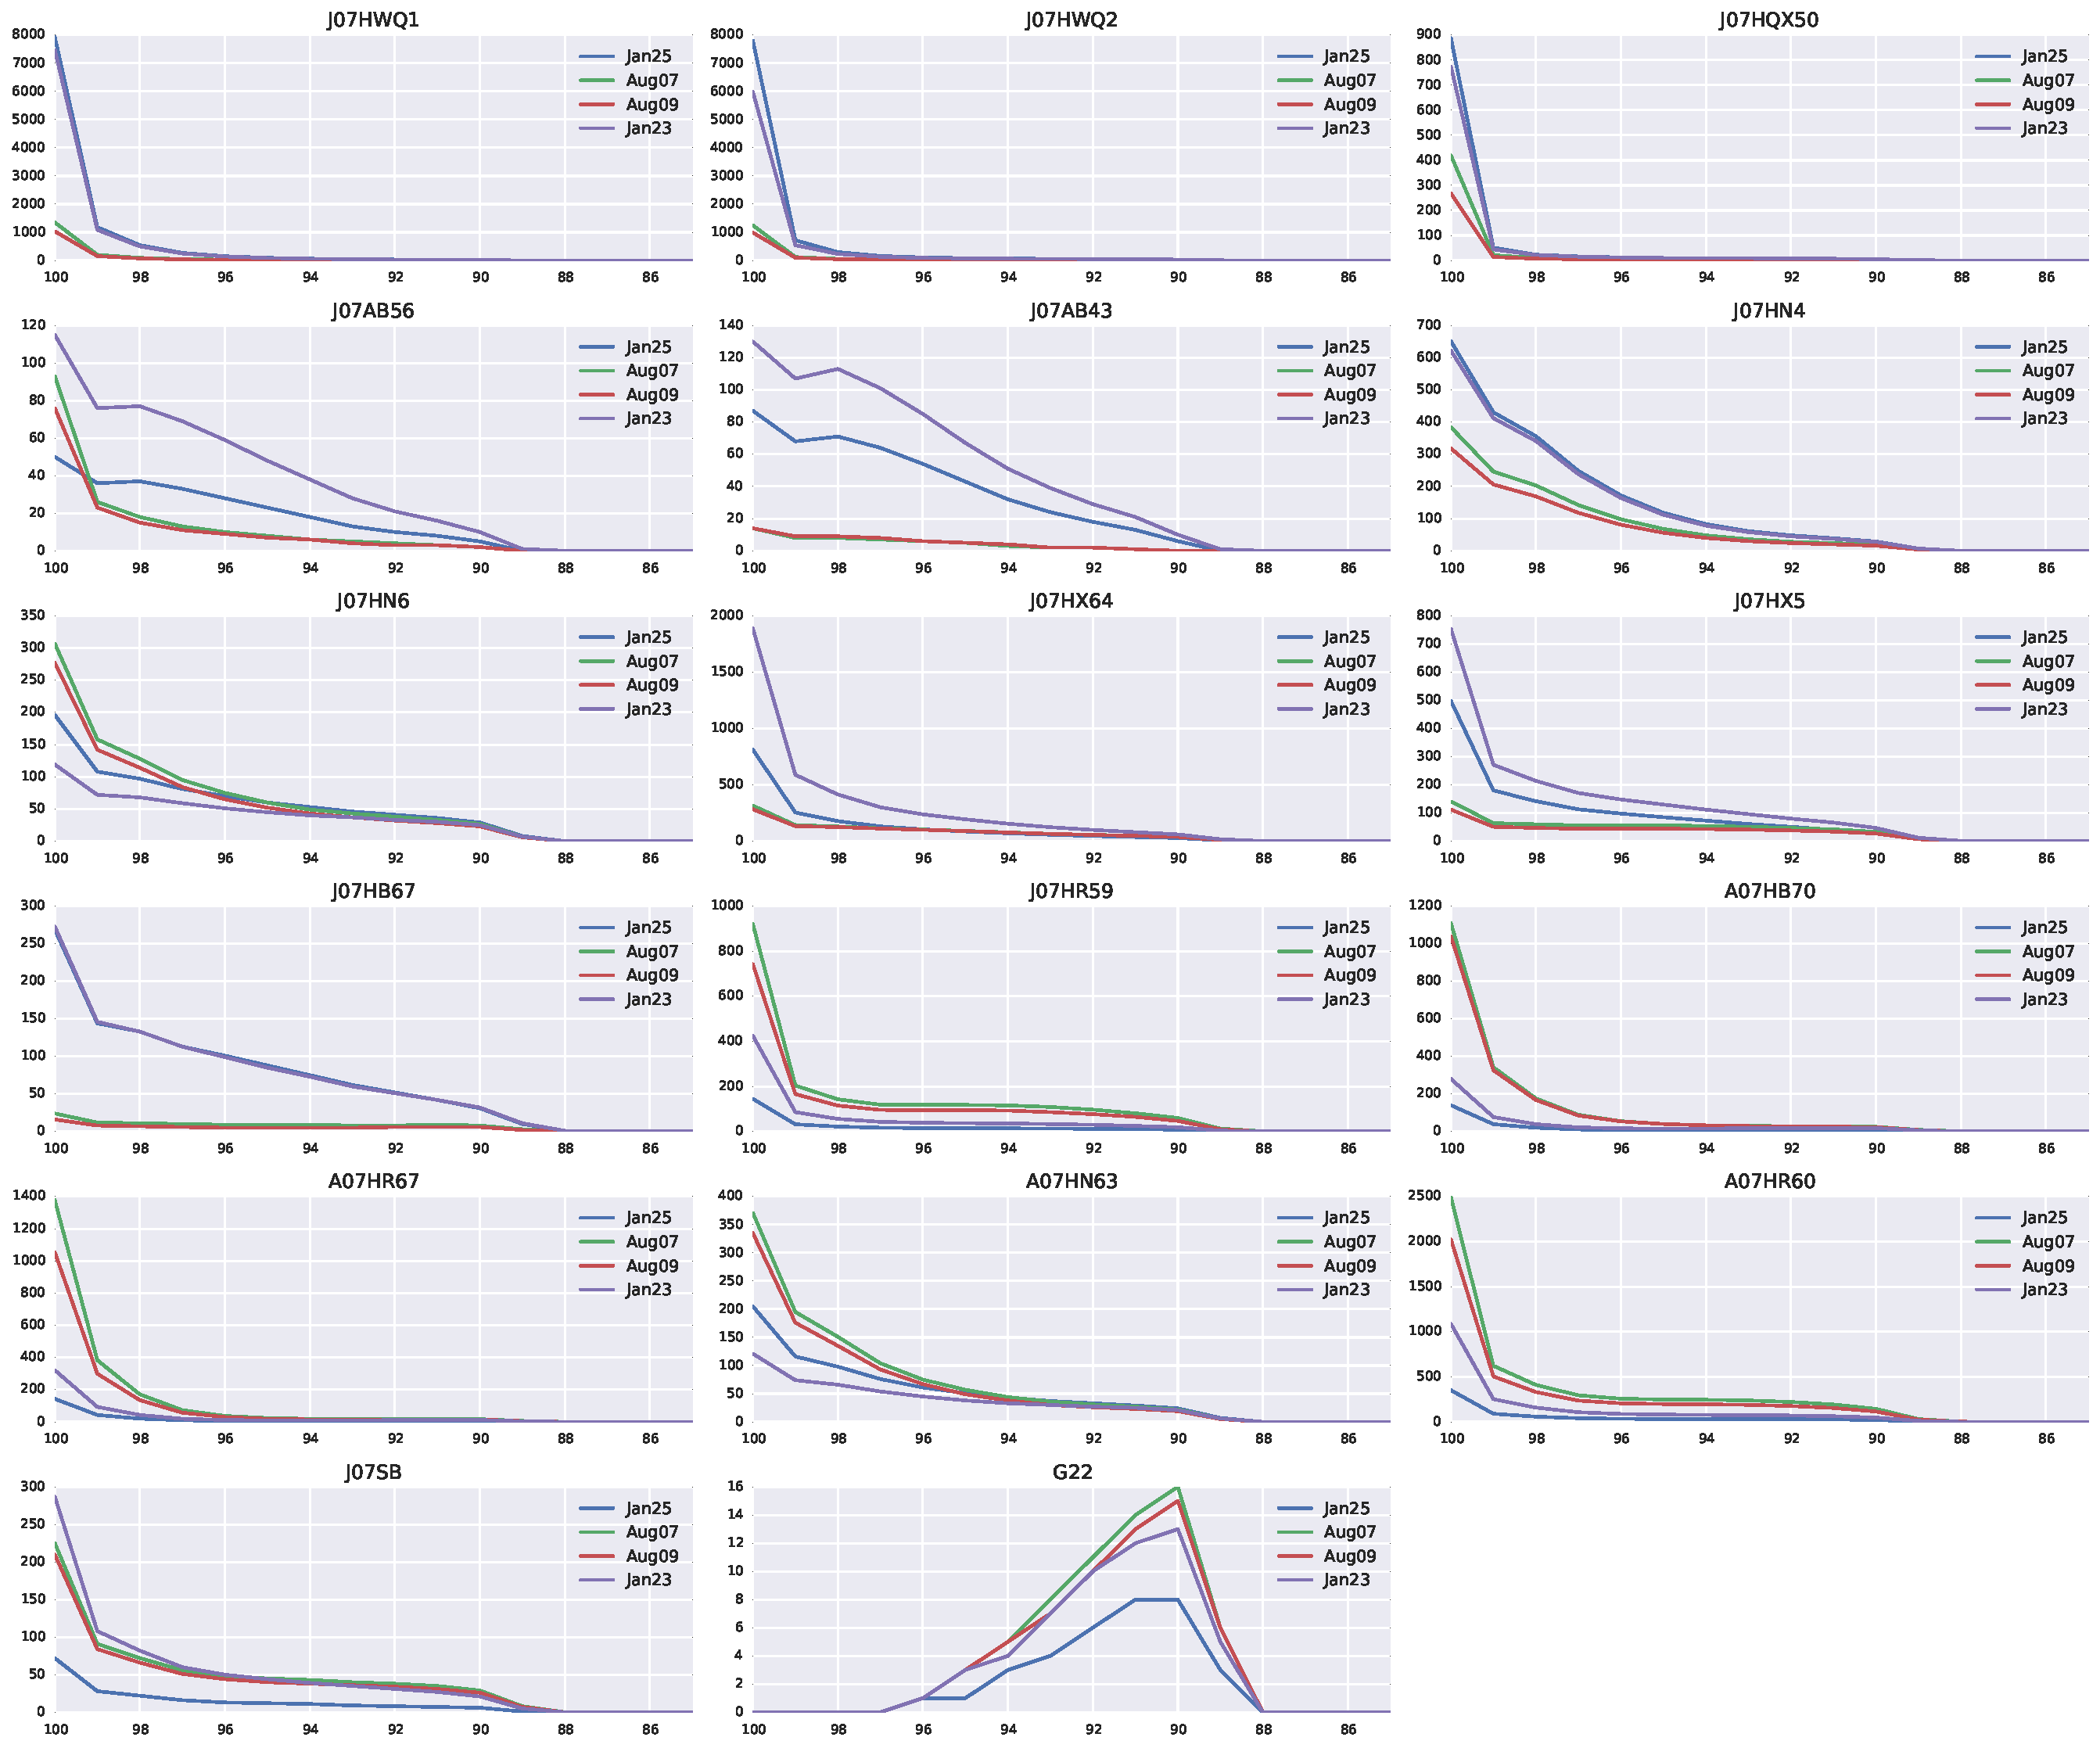
\includegraphics[width=\textwidth,height=0.9\textheight,keepaspectratio]{/Users/juan/Dropbox/GeneticVariationLT/Figures/GenomeIdentityPlots.pdf}
  \caption{Total number of recruited reads, grouped by sequence identity. The X axis shows the identity of the read to the reference genome (\%), while the \textbf{Y} axis shows the number of reads recruited at that identity (thousands of reads).}
  \label{GenomeReadIdentity}
\end{figure}


%%%NEW SUBSECTION
\clearpage
\subsection{Taxonomic Classification of Mapped and Unmapped Reads}

Before continuing with a more detailed analysis of the genetic heterogeneity present in the Lake Tyrrell microbial community, we need to address the results of the read mapping to the reference genomes. With the deep level of coverage of the community achieved with the four libraries (approximately 6 billion nucleotides in each library), this dataset represents not only the most abundant members of the community, as represented in the reference genomes used for mapping, but also allows the possibility of discovering novel organisms in the unmapped sequences \cite{Narasingarao:2012kp,Albertsen:2013gpa}. To provide an overview of the differences between the set of mapped and unmapped reads, the software Phylosift  \cite{Darling:2014ej} was used to generate a taxonomic classification of both sets of reads. An example of these results is shown in Figure \ref{Jan23_Tax} for the sample collected on January 23. In the case of the mapped reads (Figure \ref{Jan23Mapped}), as expected the majority of the reads were classified as \textit{Haloquadratum} followed by the \textit{Nanohaloarchaea}. There are also hits to organisms that were not present in the reference genomes, such as \textit{Natronema}, something that can be explained by the size of the reads (100 bp. ), which could generate spurious hits against more distantly related species at highly conserved genomic regions. In contrast, the set of unmapped reads (Figure \ref{Jan23Unmapped}) shows a broad diversity of taxonomic groups, including groups not present in the reference genomes, such as \textit{Natronomonas}, but also groups that are present, such as \textit{Salinibacter} and the \textit{Nanohaloarchaea}. This suggests that the diversity of these groups is higher than expected and is not solely represented by what is present on the reference genomes used for mapping. This also highlights the potential for the recovery of novel genomic sequences, either from this group or from novel representatives from other archeal genera.

To evaluate the differences in taxonomic composition between the set of mapped and unmapped reads, the Phylosift results were evaluated using an edge principal component analysis (EPCA), which takes into account the phylogenetic composition (similar to Unifrac distances) \cite{Matsen:2011wn}. Looking at the first two components (Figure \ref{EPCA_results}) shows that based on the predicted taxonomic composition of all the libraries, the reads separate between the mapped and unmapped groups in addition of a separation by sample (January versus August) in the case of the unmapped reads. Technical problems limited the analysis of two of the datasets from the mapped reads, so the only conclusions that can be made currently concern the separation between the unmapped and mapped reads.

As mentioned earlier, the taxonomic analysis suggests that indeed there are novel groups in the unmapped reads that are not represented in the reference genomes. This also includes the presence of viral sequences, which were not taken into account in the taxonomic analysis and likely compromise a large percentage of the sequences present in each of libraries \cite{RodriguezBrito:2010in,Emerson:tk}. Further work should include viral markers in the taxonomic classification, and mapping the sequences against available viral genomes. Nevertheless, by using the current set of reference genomes, some of the most abundant members of this community are being explored, and this information can be used to explore the genetic diversity present in the community by using a set of already validated habitat-specific genomes.

%Figure Phylosift results
\begin{figure}[!hbtp]
\centering
\subfloat[Mapped reads]{
    \label{Jan23Mapped}
    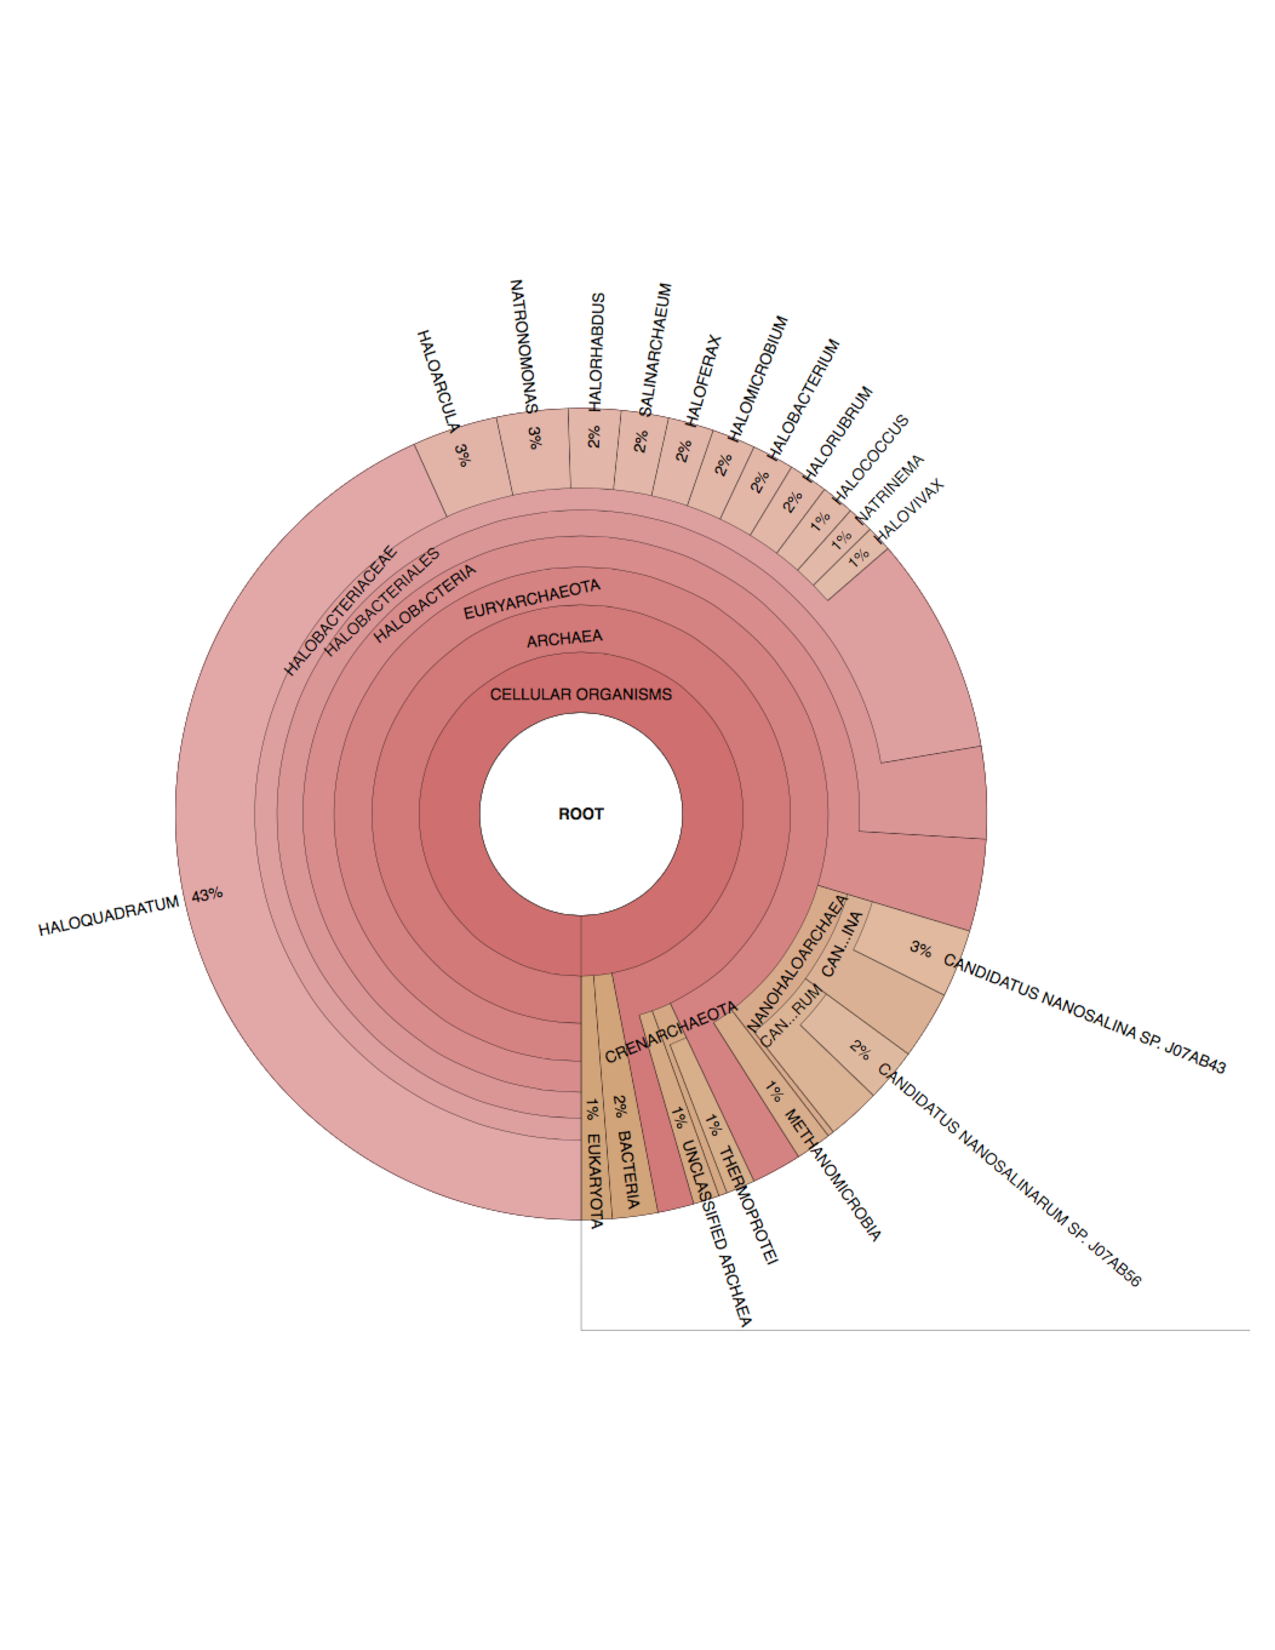
\includegraphics[width=0.7\textwidth]{Chapter5/Figures/Jan23_Mapped.pdf}
    }
    \hfill
\subfloat[Unmapped reads]{
    \label{Jan23Unmapped}
    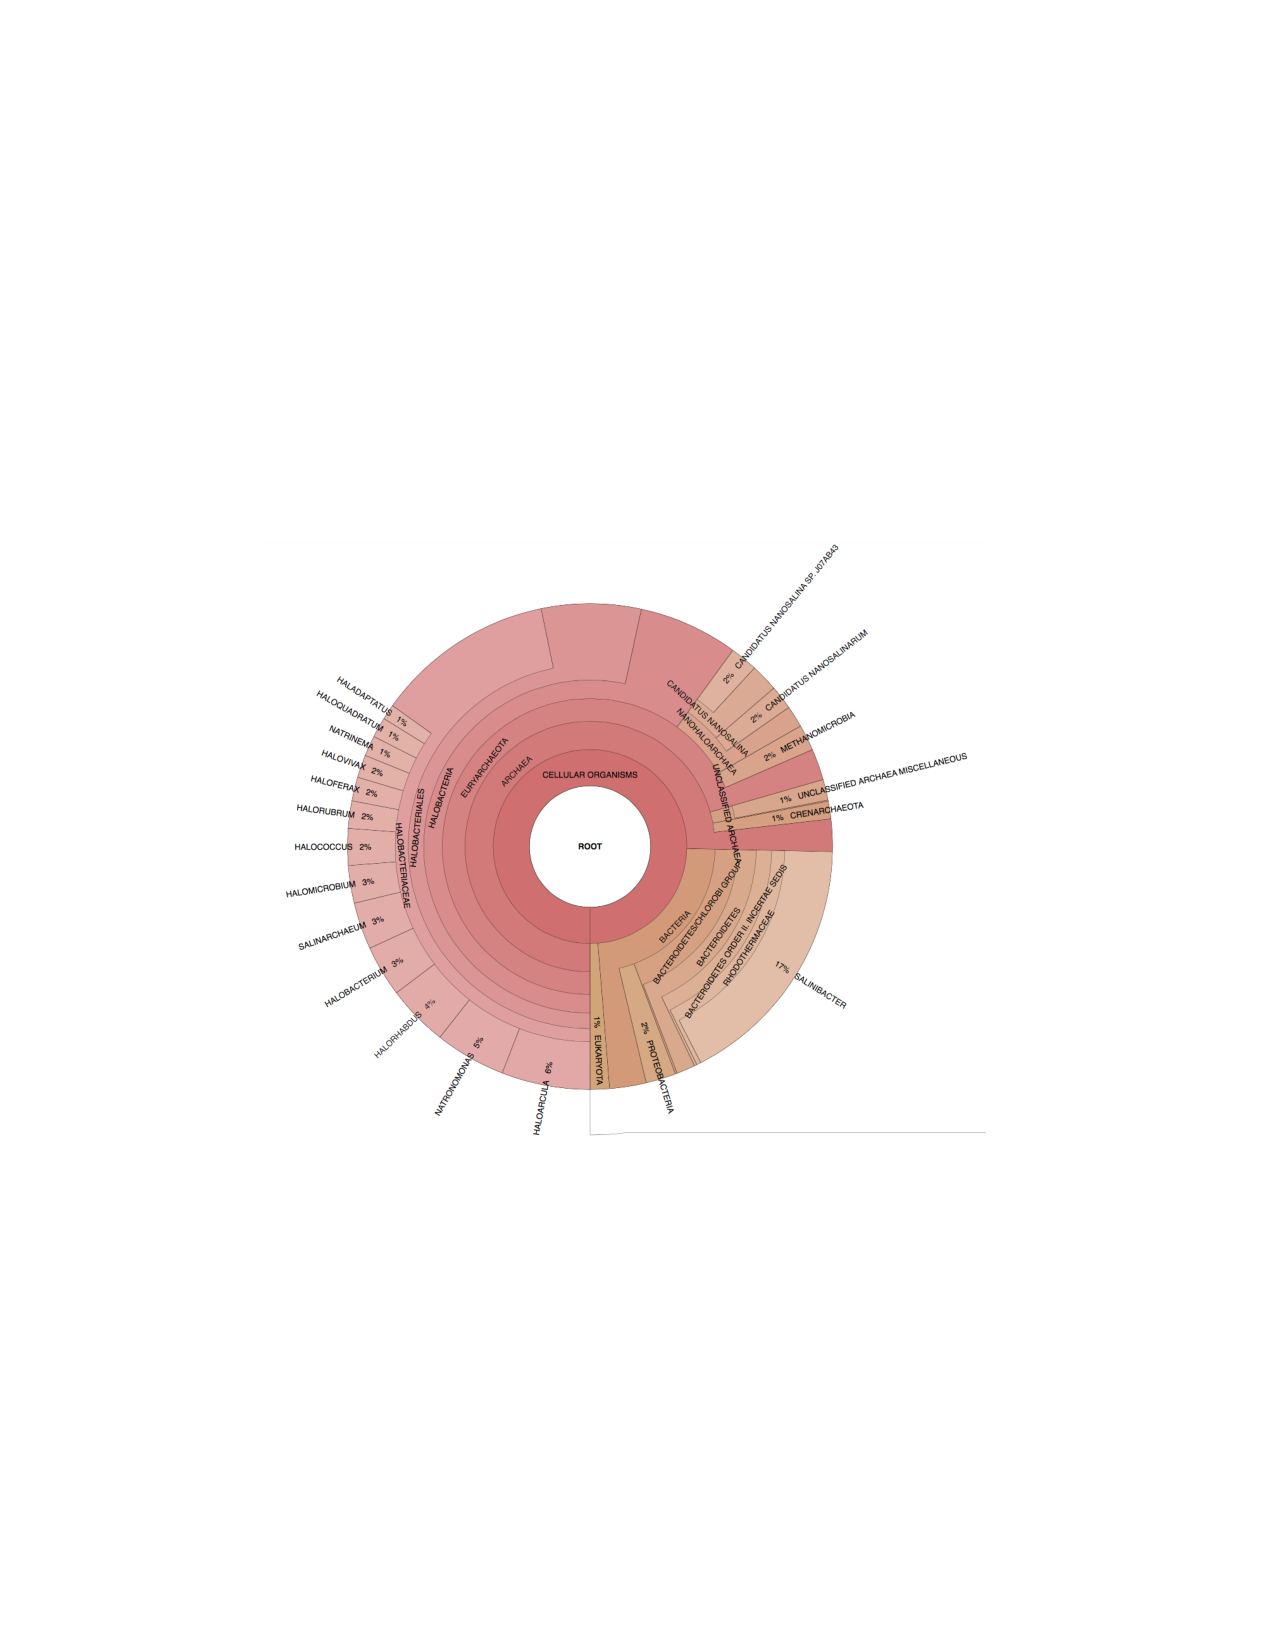
\includegraphics[width=0.7\textwidth]{Chapter5/Figures/Jan23_Unmapped.pdf}
    }
    \caption{Taxonomic classification of the mapped and unmapped reads using Phylosift \cite{Darling:2014ej}}
    \label{Jan23_Tax}
\end{figure}

%Figure Phylosift EPCA
\begin{figure}[hbt]
  \centering
  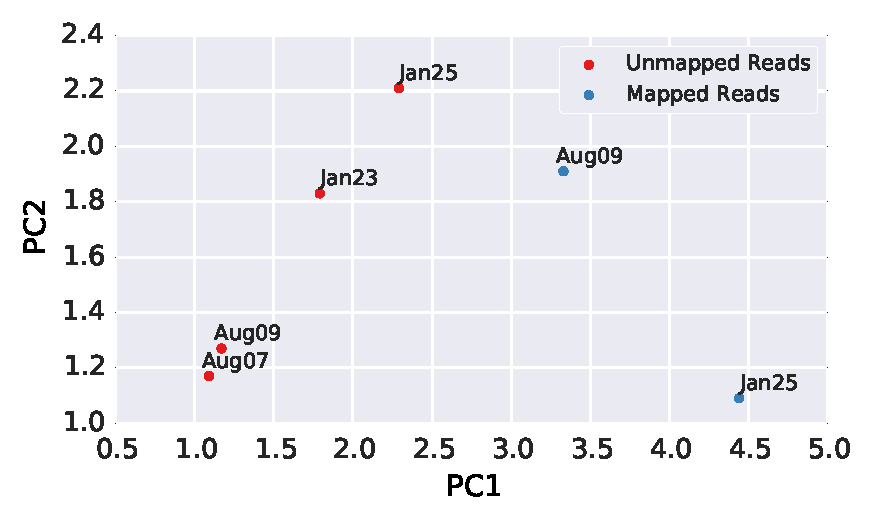
\includegraphics[width=\textwidth]{Chapter5/Figures/Unmapped_Mapped_EPCA.pdf}
  \caption{Edge principal component analysis (EPCA) of the taxonomic classification of each library.}
  \label{EPCA_results}
\end{figure}


%%%%%%%%%%%%%%%%%%%%%%
\clearpage
\subsection{Differential Coverage of Genomes and Genes}

As mentioned in the previous sections, the number of mapped reads to each of the reference genomes and the genome coverage (Tables \ref{ReadRecruitmentGenome} and \ref{ReadCoverageGenome}), suggests differences in the relative abundance of some of the populations between sampling times (January versus August). For example, the genomes of \textit{Haloquadratum} microorganisms (J07HWQ1 and J07HWQ2) recruited more reads from the January samples than from the August samples. By comparison, the reference genomes that were assembled from the August samples \cite{Podell:2013fp}, such as A07HR60, recruited more reads from the August libraries. However, just looking at the total coverage of a genome does not provide a complete picture because it is possible that some regions have higher coverage than other regions.

This differential coverage can be analyzed from two perspectives if we consider the comparison between January and August samples (combining the two individual dates for each season). From the analysis within each month, some regions may show depths of coverage that are lower than the rest of the genome. This suggests the presence of multiple strains within that particular organism where only some of the members of the population have that particular region \cite{Pasic:2009bo,Legault:2006kh,Allen:2005dg}. This has been shown in the case of \textit{Haloquadratum} \cite{Legault:2006kh} and \textit{Salinibacter} \cite{Pasic:2009bo}, using reference genomes and mapping reads from different environments to show the presence of these metagenomic islands. The second perspective is to compare the coverage of each genome between the January and August samples to look for regions of differential coverage (higher in one sample versus the other).

To evaluate this differential coverage within and between samples, the identity and coverage of all the reads along each one of the reference genomes was evaluated. This was done for both January and August samples (Appendix \ref{AppendixCoverage}). This approach allows the identification of regions with low coverage, suggesting a region only present on a subset of the strains of the populations, as well as the differential coverage between January and August. In addition, changes in the relative abundance of each gene were incorporated with the goal of identifying differential covered genes (not only regions). Looking at the individual genes allows the identification of any possible functional processes that are more abundant in one sample versus the other.

As expected, the coverage plots indicate that for some of the reference genomes, there are differences in the coverage along the genomic sequence (Appendix \ref{AppendixCoverage}). For example, in the case of the \textit{Nanohaloarchaea} J07AB56 (Figure \ref{J07AB56coverage}), there are two regions that appear with a higher coverage in the August samples with genes that have a differentially higher coverage in this sample. Looking in more detail, within the first region, genes encoding for hypothetical proteins (several of them with homology to halophages), DNA-primases and replication proteins were found. This region is located within the largest scaffold of the J07AB56 genome, suggesting that is indeed part of the genome. A possible hypothesis is that this region constitutes a halovirus that is carried as a prophage, but was released on the August sample (maybe due to environmental changes) \cite{Porter:2007jw}. The second region has genes encoding for proteins that take part in detoxification mechanisms, such as ABC transporters for xenobiotics and oxidoreductases, involved in the degradation of xenobiotics. In addition, several hypothetical proteins can be found in this region.

%“The second region has genes encoding for defense mechanisms, such as ABC transporters and oxidoreductases, besides hypothetical proteins.”  How are ABC transporters and oxidoreductases components of defense mechanisms?  


A summary of the differential recruitment of the reads at the gene level is shown in Figure \ref{CoverageGenes}, which indicates that in the case of the reference genomes that were recovered from the January samples, the majority of genome genes indeed recruited to reads from the January Illumina libraries. Some exceptions to this are in the \textit{Halonotius} J07HN6 genome, which has a large fraction of the genes recruiting more reads from the August libraries than from the January ones. It is possible that this organism is present and abundant in the August samples, but it was not previously assembled. Also the \textit{Halonotius} J07HN6 and A07HN63 are very similar \cite{Podell:2013fp}, which could also explain the higher differential coverage.

The idea of looking at the differential coverage of the genomes and the  comparison between multiple samples is not new in the literature \cite{DyallSmith:2011tu,Pasic:2009bo}, as it provides a broad picture of the possible strain variation that is present for each of the populations under study. To our knowledge, the idea of using RPKM values, commonly used in gene expression studies \cite{Mortazavi:2008jj}, and applying it to comparisons to metagenomic samples is indeed a novel one. Although a broad picture of the differences was presented here, further work will focus in specific populations, such as the \textit{Haloquadratum} genomes, and will also include the use of available isolate genomes \cite{DyallSmith:2011tu}.

%Figure Gene differences season
\begin{figure}[!hbtp]
  \centering
  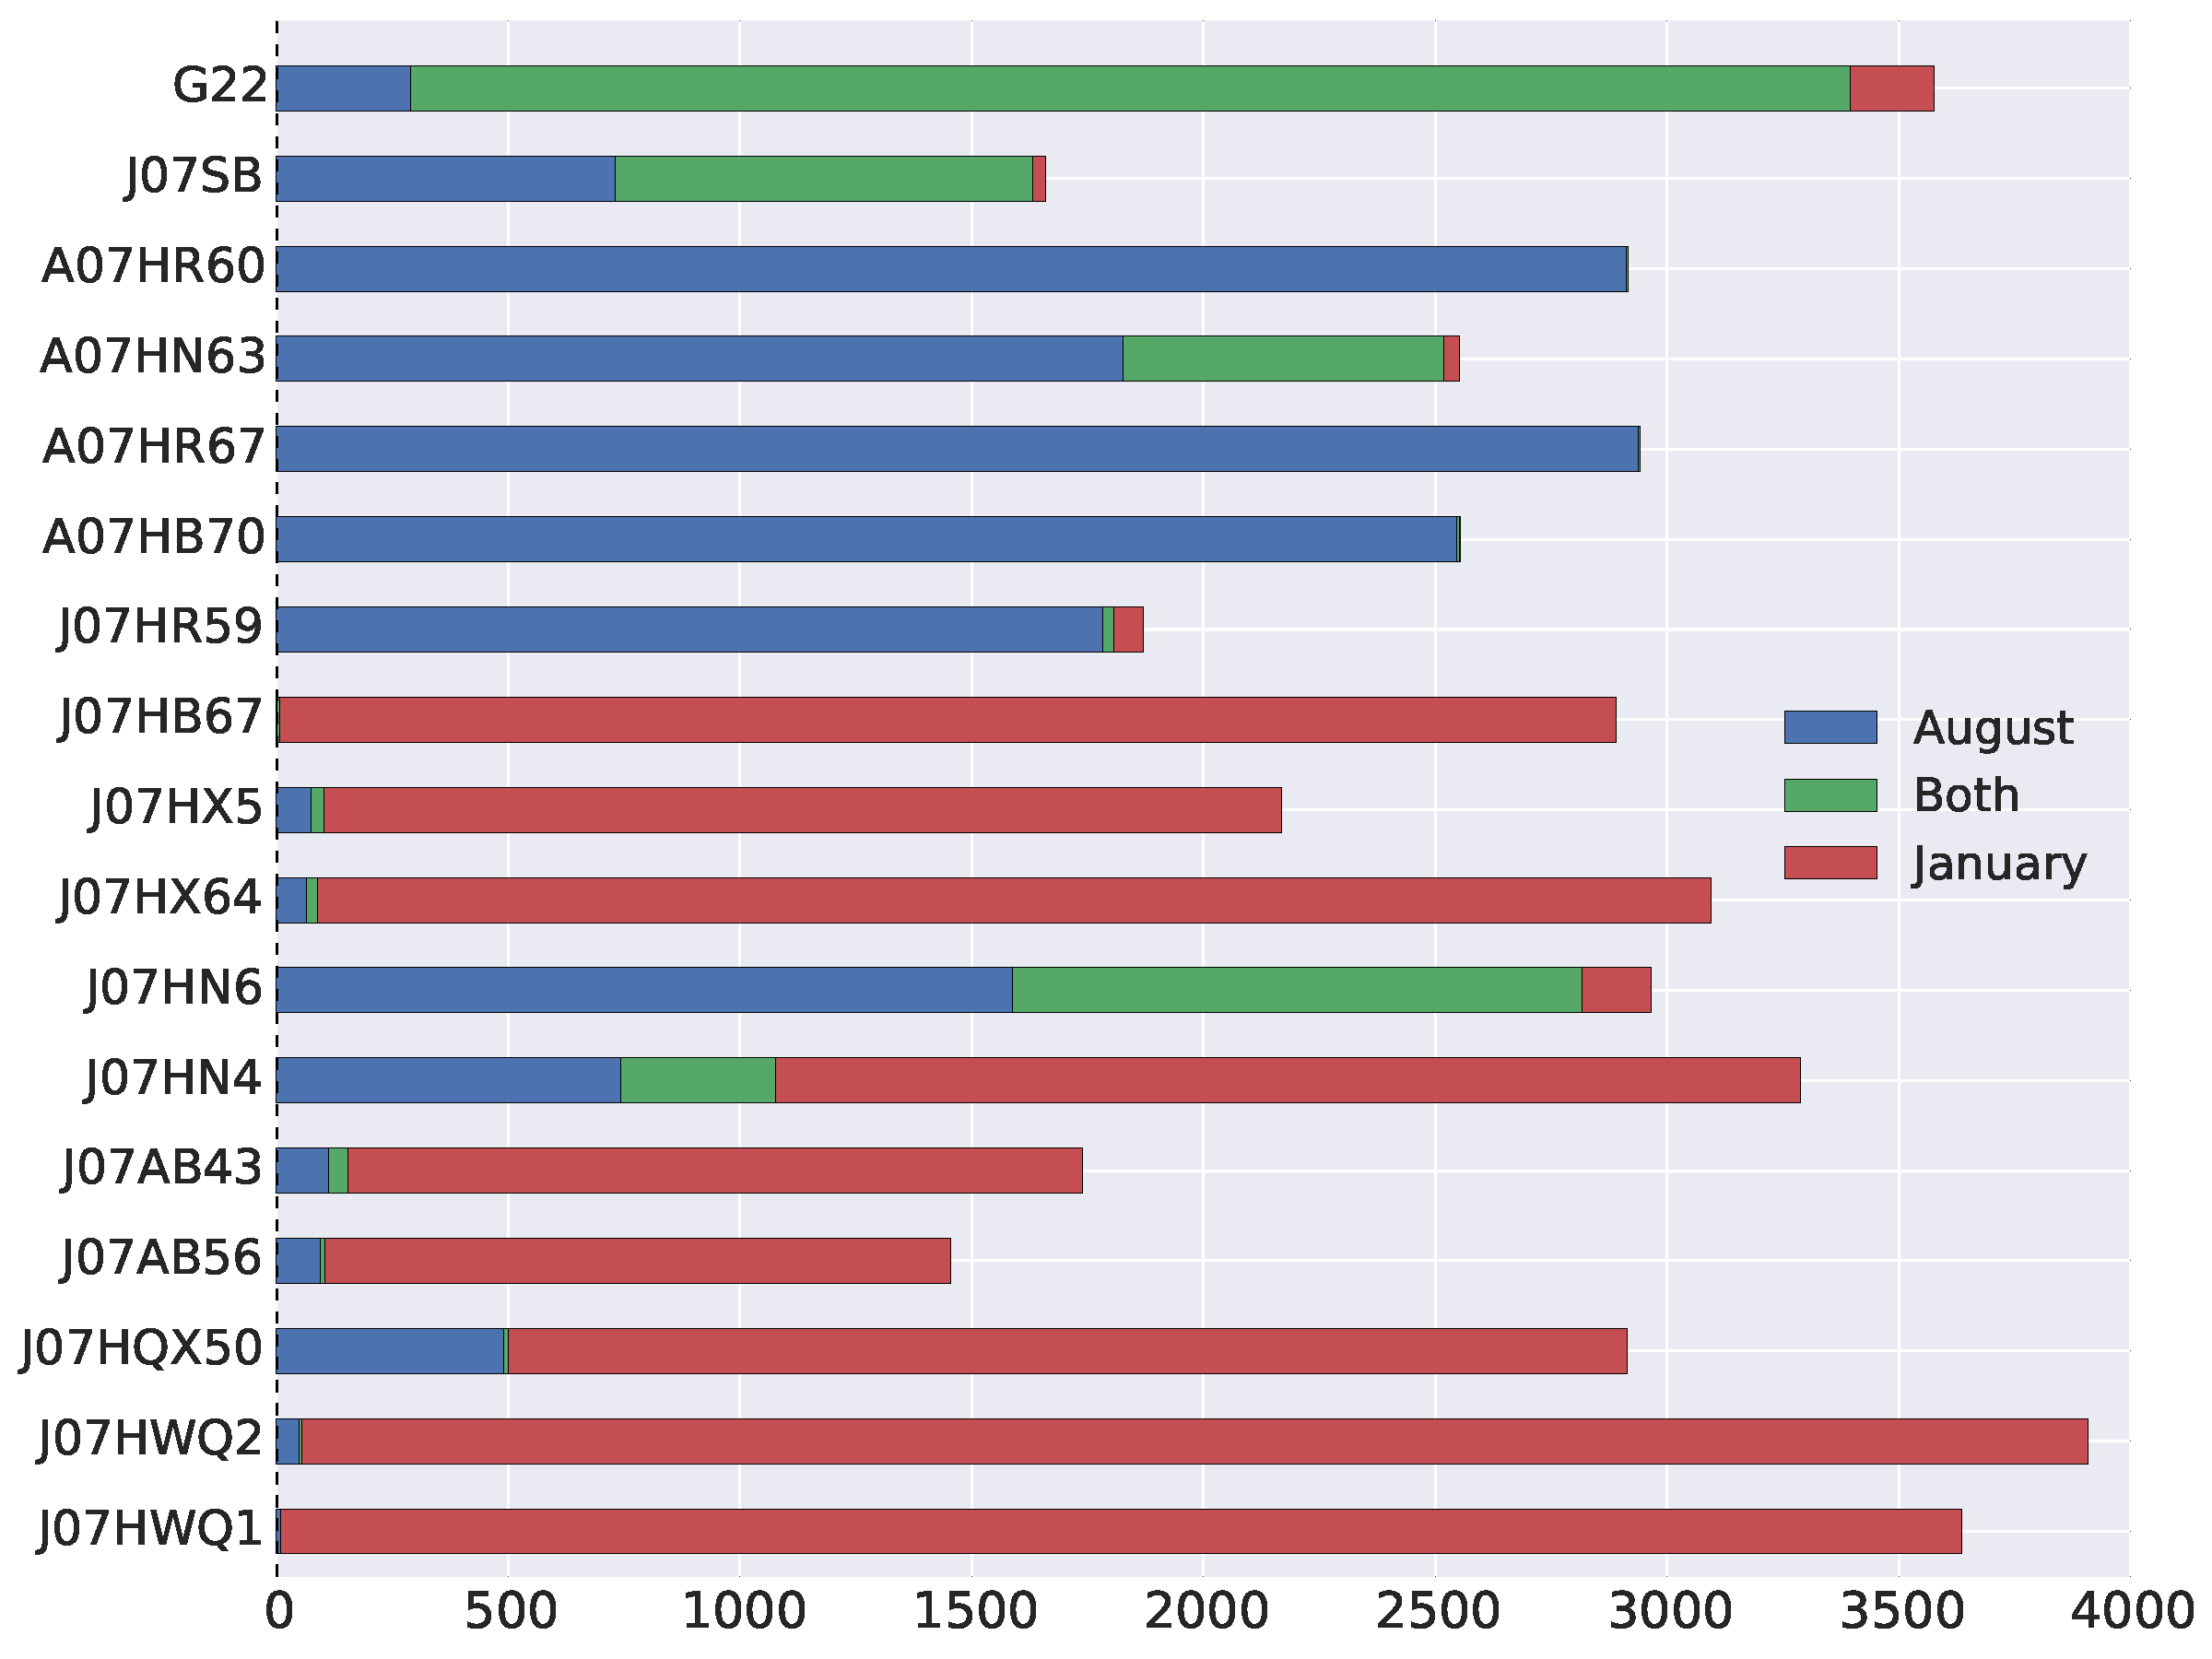
\includegraphics[width=0.7\textwidth]{Chapter5/Figures/GeneDifferencesSeason.pdf}
  \caption{Number of genes that differentially recruited reads from either the January or August libraries, in each of the reference genomes. A two-tailed Fisher Exact test (p-value $<$ 0.05) was used to determined the differences between samples. \textit{Both}, indicates genes that were not found to be significantly more abundant in either of the samples.} 
  \label{CoverageGenes}
\end{figure}

%%%%%%%%%%%%%End of Section
\clearpage
\subsection{Fine-scale Genetic Variation: Single Nucleotide Polymorphisms (SNPs)}

The genetic heterogeneity that is present in each of the reference populations can be explored in more detail by leveraging the information provided by the reads and the high depth of coverage of each of the genomes (with the exception of G22). With this, it is possible to quantify the nucleotide variation in each genome (single nucleotide polymorphisms, SNPs) and to evaluate the effects of such variation at the functional level. Other types of variations, such as insertions, deletions, and structural variants, can be analyzed as well, but the current goal is to evaluate the evolutionary forces that are generating such variation. Under such an evaluation, the emphasis will be on the polymorphisms that act on protein-coding sequences.

For variant calling, only high-quality SNPs were considered in the analysis, filtering the alignment files priors to SNP calling with Freebayes. Only those sites with a quality score of 20 or more and a mapping quality score of 30 or more were selected in the analysis, similar to methods employed in other studies \cite{Schloissnig:2012hx}

The number of SNPs/Kb on each of the genomes is shown on Table \ref{SNPS_KB}, indicating differences on the number of SNPs when comparing the different references. Within each of the genomes, there are small differences within each season sample (January 23 \& January 25, August 7 \& August 9), but there are differences between the January and August samples. The \textit{Nanohaloarchaea} genomes exhibit the largest number of SNPs/Kb among all the genomes in the January libraries, but it is lower on the August libraries. Comparing the number of SNPs/Kb found on each library, we can visualize that all four of them are within similar ranges (Figure \ref{BoxplotSNPsKB}) with averages between 4-5 SNPs/Kb.

Although from the visual inspection of Table \ref{SNPS_KB} it does not appear that there is any relationship between those genomes that recruited more reads and the number of SNPs, this needs to be evaluated. When comparing the depth of coverage of each reference genome versus the number of SNPs/Kb found in each of the libraries (Figure \ref{SNPsCoverage}), there is no relationship between these two variables. This was confirmed by testing with the Spearman correlation coefficient for the combined libraries (coefficient: 0.16, \textit{pvalue}: 0.21). This strongly suggests that the differences in SNPs numbers are due to the genetic diversity found in each of these reference genomes, where organisms such as the \textit{Nanohaloarchaea} J07AB43 and J07AB56 have higher rates of genetic diversity (more strain diversity) compared to organisms such as J07HWQ1 or J07HWQ2.

The effect of each variation within the genome can be evaluated in more detail by quantifying those SNPs that were intergenic or located within a coding region. In the latter case, this variation could be either synonymous (no amino acid change) or non-synonymous (change in the resulting amino acid). For each of the genomes, no differences between libraries in the percentage of intergenic, non-synonymous, and synonymous SNPs (Figure \ref{SNPsummary}) were observed; the exception was the G22 genome, but the overall coverage and percentage of SNPs for this genome are low. The distribution of SNPs for all the genomes (Figure \ref{BoxPlotSNP}) shows that the majority of the SNPs are located in coding sequences and are synonymous. Also, it is interesting to observe the dispersion on the data, where for the case of the non-synonymous SNPs, the distribution goes between 20-30\%, while in the case of intergenic SNPs, it moves between 15-37\%. These can be observed more in detail on Table \ref{TypeSNP_SummaryGenome} where on one extreme there are genomes from the \textit{Haloquadratum} group with over 30\% of the SNPs within intergenic regions, and on the other side the \textit{Nanohaloarchaea}, with ~10\% of the SNPs within intergenic regions. This can be explained by the differences in genome size, where \textit{Haloquadratum} organisms have large genomes (over 3 Mb.), and the \textit{Nanohalorachaea} have smaller genomes (1.8 Mb) with reduced intergenic space \cite{Narasingarao:2012kp,Podell:2013kx}. Overall, the percentage of non-synonymous substitutions for all the genomes was similar, something expected given the characteristics of this type of change, which modifies the amino acid sequence and can led to non-functional organisms. Compared to values observed in other metagenomic studies (focusing only on a few species), the trends observed are similar, but with higher rates of synonymous substitutions compared to non-synonymous ones \cite{Simmons:2008by}.

The sampling strategy allows us to ask two different questions in terms of the temporal variation between the samples. The first comparison is a variation within each sampling month (January and August) between the samples collected two days apart. The second comparison is between the two different seasons (January vs August). By looking at the SNPs found on each of the samples, we can look whether the SNPs found are unique to each one of the libraries or there are similarities between time points. We can visualize the differences using Venn diagrams to compare the different sampling dates. The comparison between the January dates (23 versus 25) (Figure \ref{VennJan}) shows that in all the reference genomes, the majority of the SNPs is shared between the two samples days. G22 is an exception due to its low coverage. A similar trend is observed in the comparison of the August 7 and August 9 libraries (Figure \ref{VennAug}),however, in contrast to the January data, the\textit{Nanohaloarchaea} genomes (J07AB56 and J07AB43) have differences between the two dates. These results suggest that different populations of these organisms may be found in the two samples. Further analysis (focusing only in these two populations) is needed to answer this question and evaluate whether these differences are indeed due to differences in population structure for these organisms \cite{Schloissnig:2012hx,Shapiro:hi,Vos:2011ux}. Both dates (January versus August) were compared using the combined set of SNPs. Interestingly, the majority of the SNPs appear to be shared between the two samples with small differences in the case of the \textit{Nanohaloarchaea} and with unique SNPs present in the January sample. This suggests that the populations found in January could be very similar to the ones present in August \cite{Doolittle:2012hf}. The same strains could be present, however the abundance of the members of the community varies. This is supported by the previous analysis of the reads that mapped to each reference genome. Exploring this phenomenon requires focusing on a few organisms, comparing not only these assembled genomes, but also genomes from other environments and/or isolates if available. In particular, measurements of nucleotide diversity, fixation index, and McDonald-Kreitman tests \cite{Schloissnig:2012hx,Simmons:2008by} should be used to evaluate differences at the population level between the members of the community. Nevertheless, the initial conclusion of both populations being similar, with only differences in their abundances, is intriguing. The slow growth rate of some of the organisms found in hypersaline communities \cite{DyallSmith:2011tu} (at least in laboratory studies) may suggest that samples of seven months apart is not long enough to provide a temporal picture of the evolution of the population structure within this ecosystem. This contrasts with what has been observed for viral communities in hypersaline communities, where rapid temporal variation has been observed  \cite{RodriguezBrito:2010in,Emerson:2012gh}.

%%Tables and Figures

%Table count of snps
\begin{table}[ht]
  \caption{Count of number of SNPs per kilobase in each of the Illumina libraries for the reference genomes.}
  \begin{tabularx}{\textwidth}{L{2.2cm}R{2cm}R{3cm}R{3.2cm}R{2cm}}
  \hline
    \textbf{Genome} & \textbf{Jan 23} & \textbf{Jan 25} & \textbf{Aug 07} & \textbf{Aug 09} \\
    \hline
     \textit{J07HWQ1} & 3.83 & 3.81 & 3.75 & 3.70 \\
     \textit{J07HWQ2} & 2.51 & 2.52 & 3.28 & 2.46 \\
     \textit{J07HQX50} & 1.44 & 1.44 & 1.42 & 1.39 \\
     \textit{J07AB56} & 10.10 & 9.71 & 4.95 & 5.21 \\
     \textit{J07AB43} & 10.75 & 10.64 & 7.30 & 7.19 \\
     \textit{J07HN4} & 9.09 & 9.09 & 9.01 & 9.01 \\
     \textit{J07HN6} & 2.87 & 2.61 & 2.85 & 2.81 \\
     \textit{J07HX64} & 9.52 & 9.43 & 9.35 & 9.26 \\
     \textit{J07HX5} & 9.26 & 9.17 & 9.09 & 9.01 \\
     \textit{J07HB67} & 9.09 & 9.17 & 6.45 & 5.24 \\
     \textit{J07HR59} & 1.36 & 1.15 & 1.54 & 1.51 \\
     \textit{A07HB70} & 7.19 & 7.04 & 7.30 & 7.30 \\
     \textit{A07HR67} & 5.85 & 5.71 & 5.92 & 5.92 \\
     \textit{A07HN63} & 1.72 & 1.98 & 2.12 & 2.10 \\
     \textit{A07HR60} & 3.79 & 3.69 & 3.91 & 3.89 \\
     \textit{G22} & 0.04 & 0.03 & 0.03 & 0.03 \\
     \textit{J07SB} & 6.06 & 5.65 & 6.10 & 6.10 \\     
  \end{tabularx}
  \label{SNPS_KB}
\end{table}

%TABLE SUMMARY TYPE OF SNPs

\begin{table}[ht]
  \caption{Percentage of the different type of SNPs on each genome}
  \begin{tabularx}{\textwidth}{L{2.1cm}R{2.3cm}R{3cm}R{3.8cm}}
  \hline
    \textbf{Genome} & \textbf{Intergenic} & \textbf{Synonymous} & \textbf{Non-Synonymous}\\
    \hline
     \textit{J07HWQ1} & 36.90 & 38.56 & 24.55 \\
     \textit{J07HWQ2} & 37.31 & 34.48 & 28.22 \\
     \textit{J07HQX50} & 31.32 & 36.95 & 31.73 \\
     \textit{J07AB56} & 10.67 & 65.96 & 23.37 \\
     \textit{J07AB43} & 10.30 & 64.02 & 25.68 \\
     \textit{J07HN4} & 15.27 & 66.28 & 18.45 \\
     \textit{J07HN6} &  19.98 & 55.62 & 23.40\\
     \textit{J07HX64} & 18.98 & 51.18 & 29.84 \\
     \textit{J07HX5} & 20.72 & 53.88 & 25.41 \\
     \textit{J07HB67} & 12.06 & 60.65 & 27.29 \\
     \textit{J07HR59} & 23.78 & 53.89 & 22.33 \\
     \textit{A07HB70} & 22.38 & 49.23 & 28.40 \\
     \textit{A07HR67} & 20.75 & 55.58 & 23.67 \\
     \textit{A07HN63} & 21.55 & 54.69 & 23.76 \\
     \textit{A07HR60} & 26.79 & 49.54 & 23.67 \\
     \textit{G22} & 15.86 & 65.34 & 17.80 \\
     \textit{J07SB} & 15.67 & 59.60 & 24.74 \\     
  \end{tabularx}
  \label{TypeSNP_SummaryGenome}
\end{table}

%FIgures. SNPs versus depth of coverage
\begin{figure}[h]
  \centering
  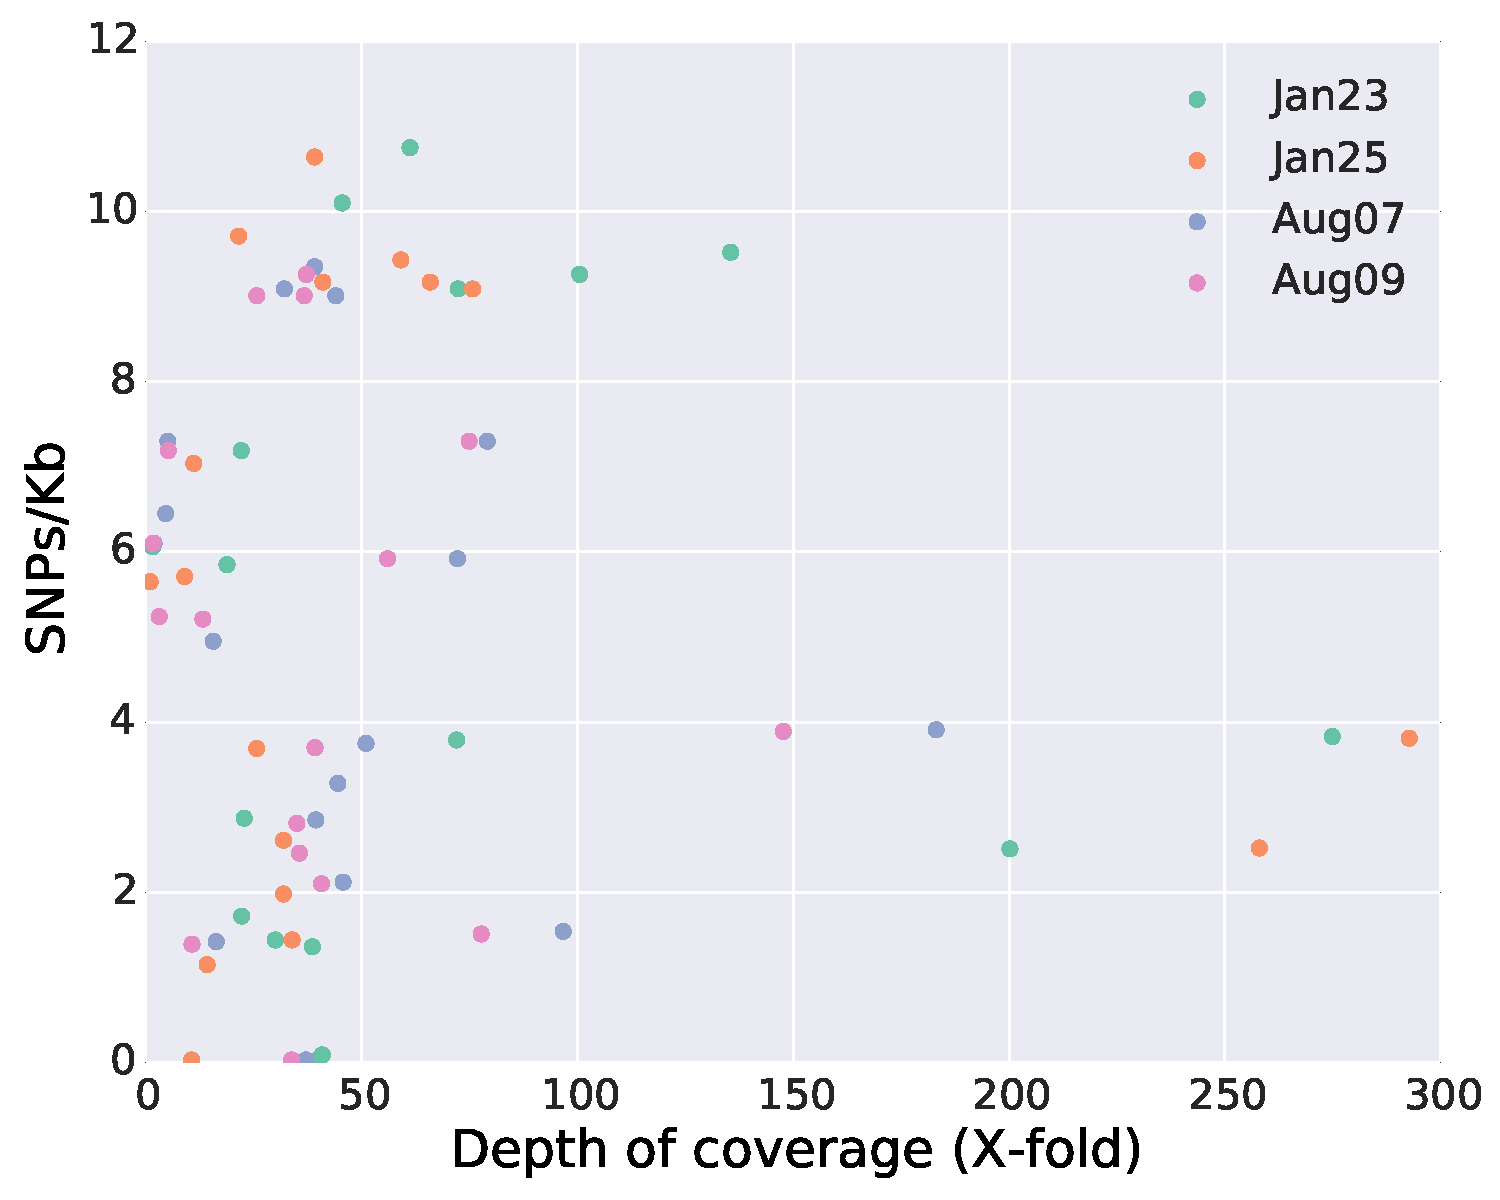
\includegraphics[width=0.7\textwidth,height=\textheight,keepaspectratio]{Chapter5/Figures/DepthCoverage_VS_SNPsKB.pdf}
  \caption{Scatterplot of depth of coverage versus SNPs/Kb for each of the reference genomes for the four libraries.}
  \label{SNPsCoverage}
\end{figure}

%
%%FIgures. Boxplot, SNPsKB
\begin{figure}[h]
  \centering
  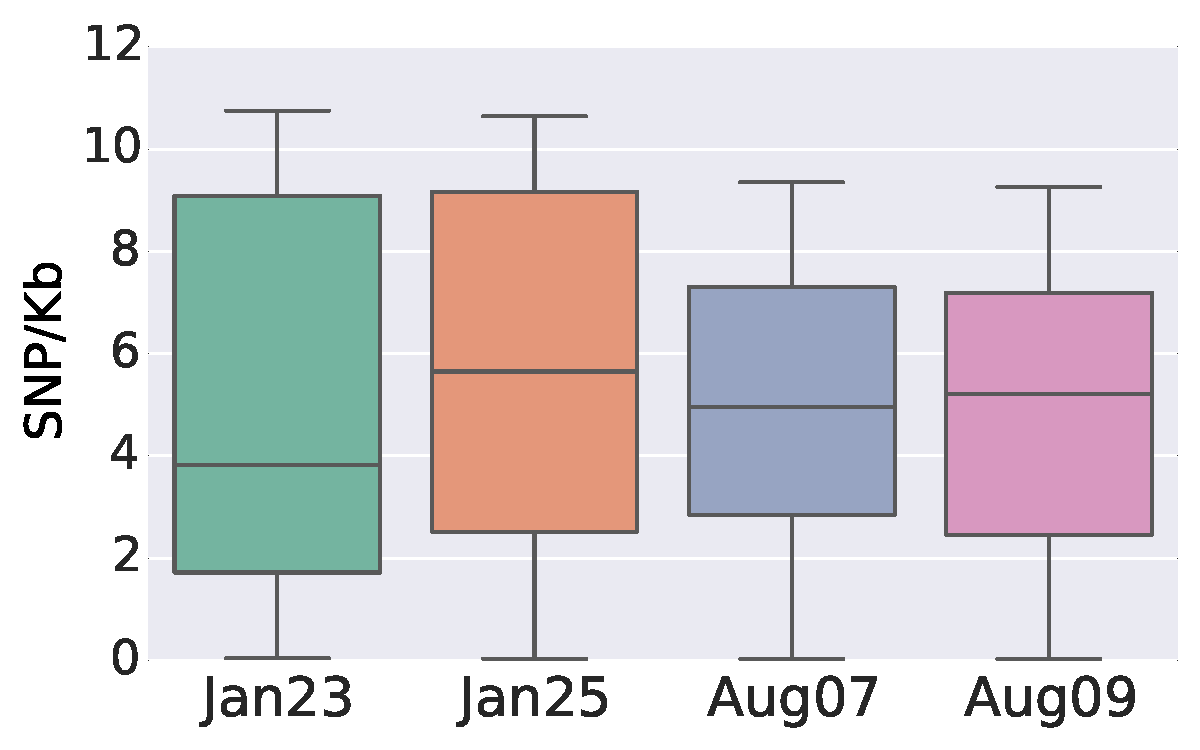
\includegraphics[width=0.6\textwidth,height=\textheight,keepaspectratio]{Chapter5/Figures/Boxplot_SNPsKB.pdf}
  \caption{Boxplot summarizing the number of SNPs/Kb for each genome, in each of the sequence libraries.}
  \label{BoxplotSNPsKB}
\end{figure}


%FIgures. SNP summary
\begin{figure}[h]
  \centering
  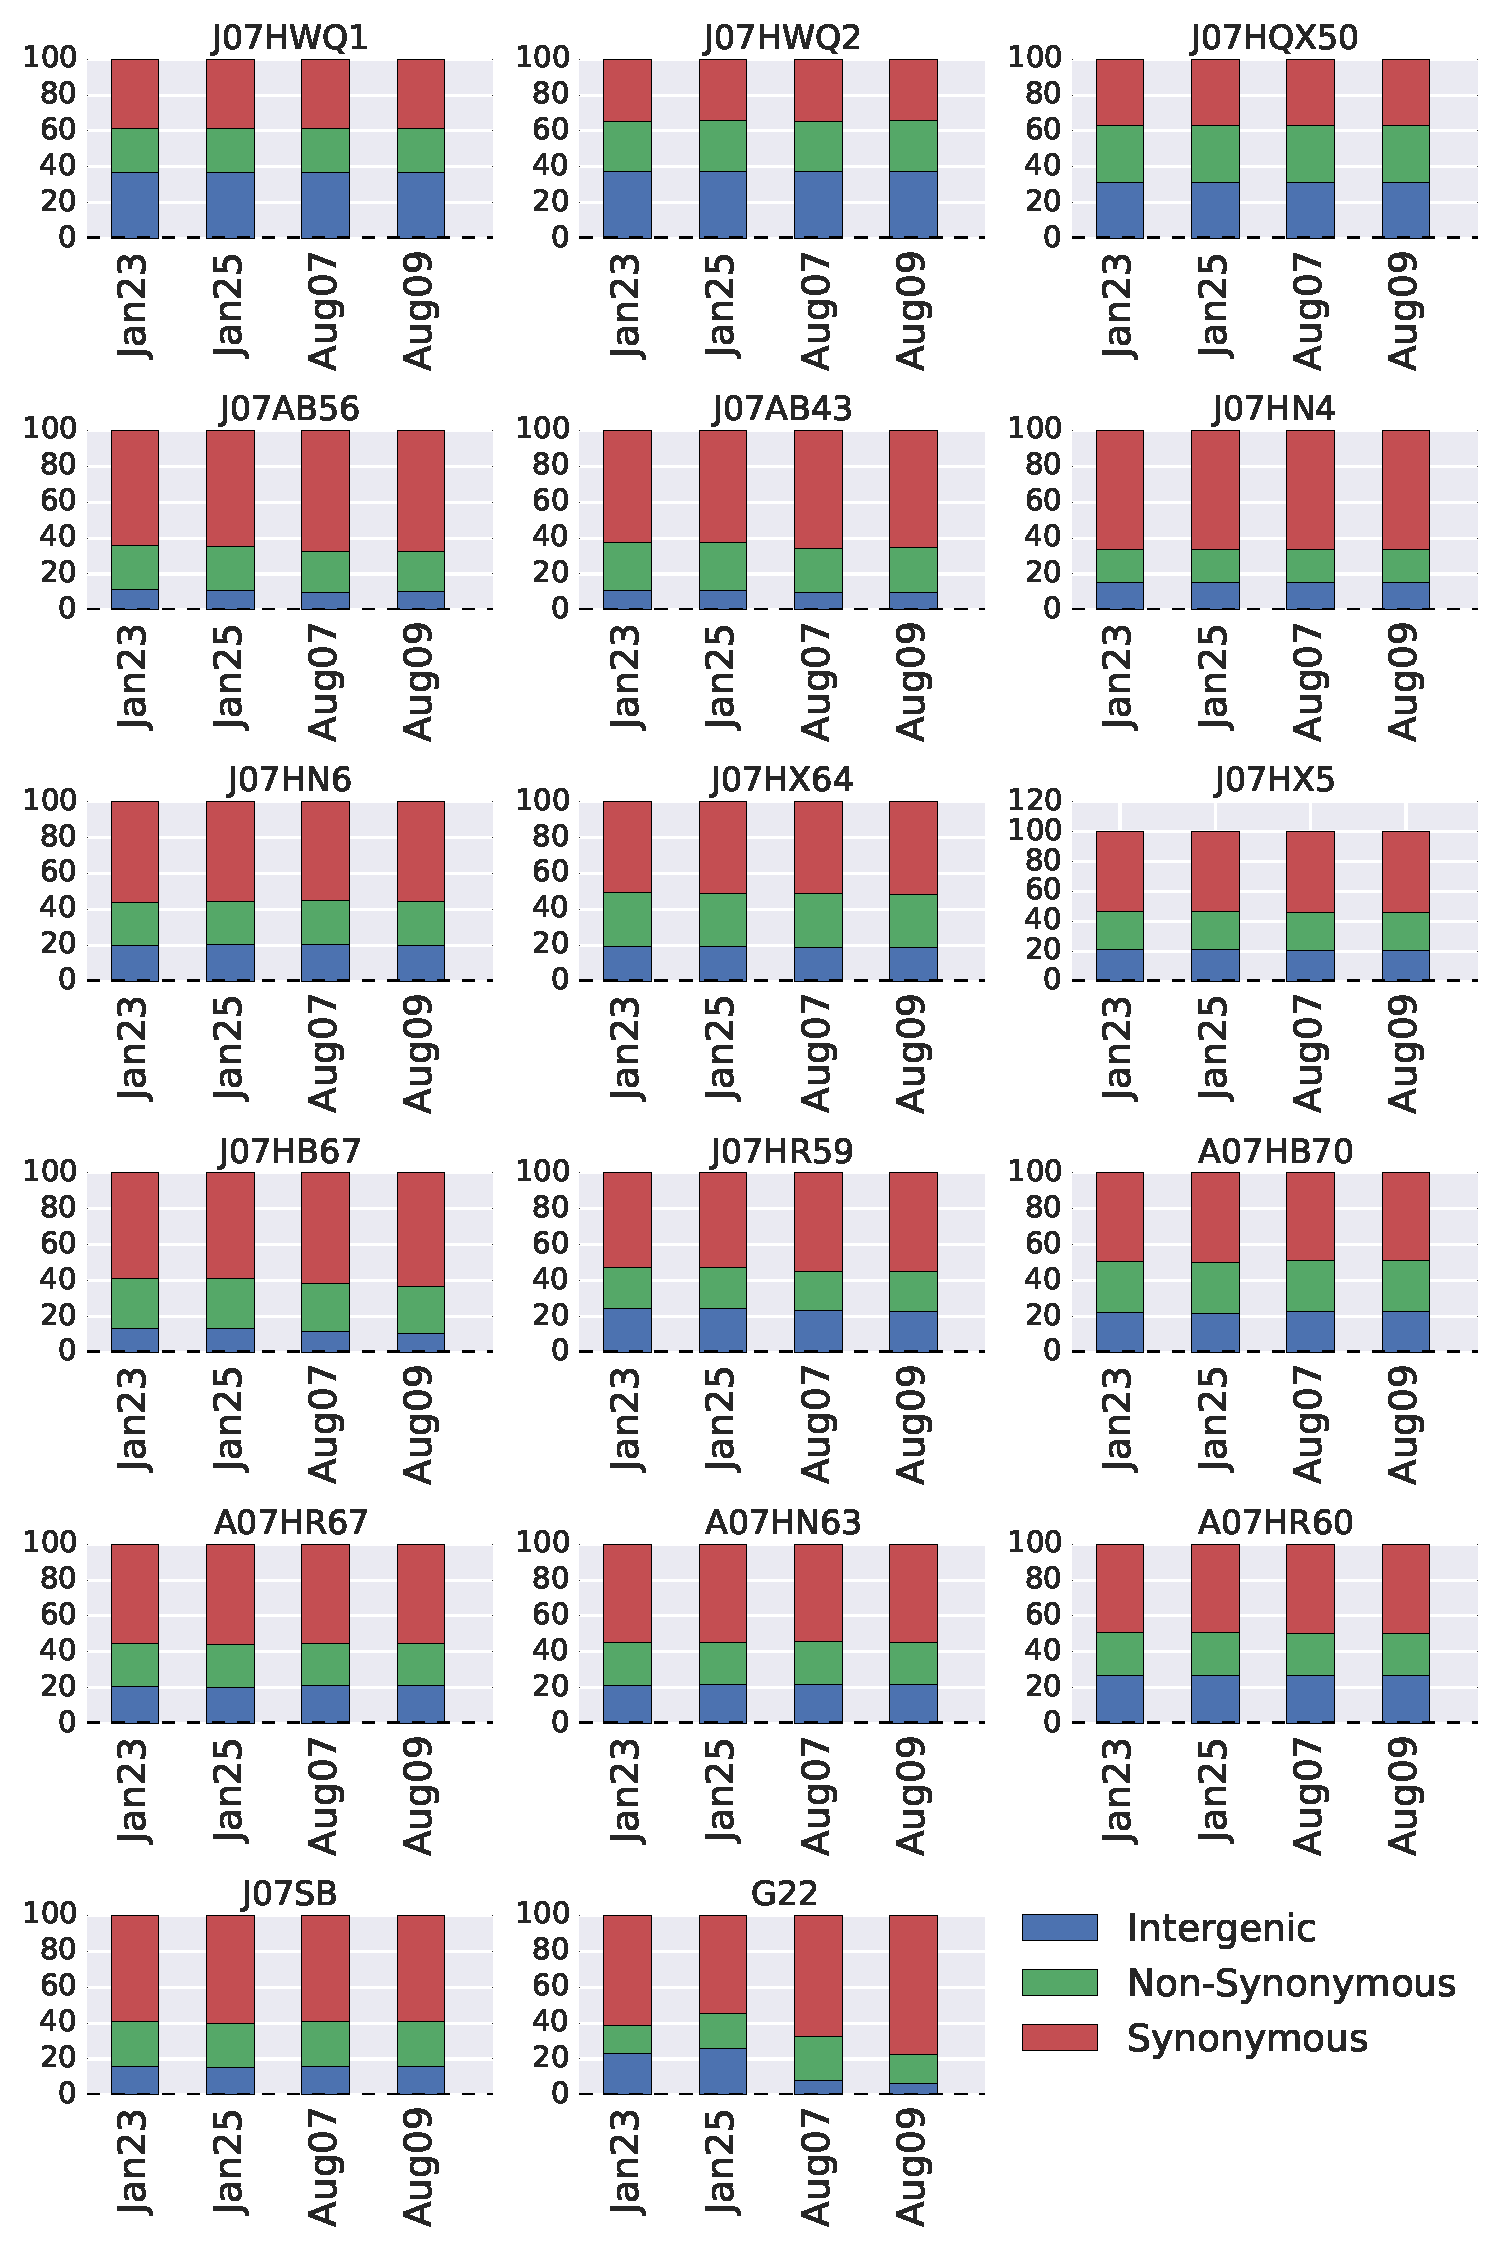
\includegraphics[width=\textwidth,height=0.8\textheight,keepaspectratio]{Chapter5/Figures/SNPsummary.pdf}
  \caption{Percentage of intergenic, non-synonymous and synonymous SNPs in each genome, for all the sequence libraries.}
  \label{SNPsummary}
\end{figure}

%Boxplot, type of SNPs
\begin{figure}[ht]
  \centering
  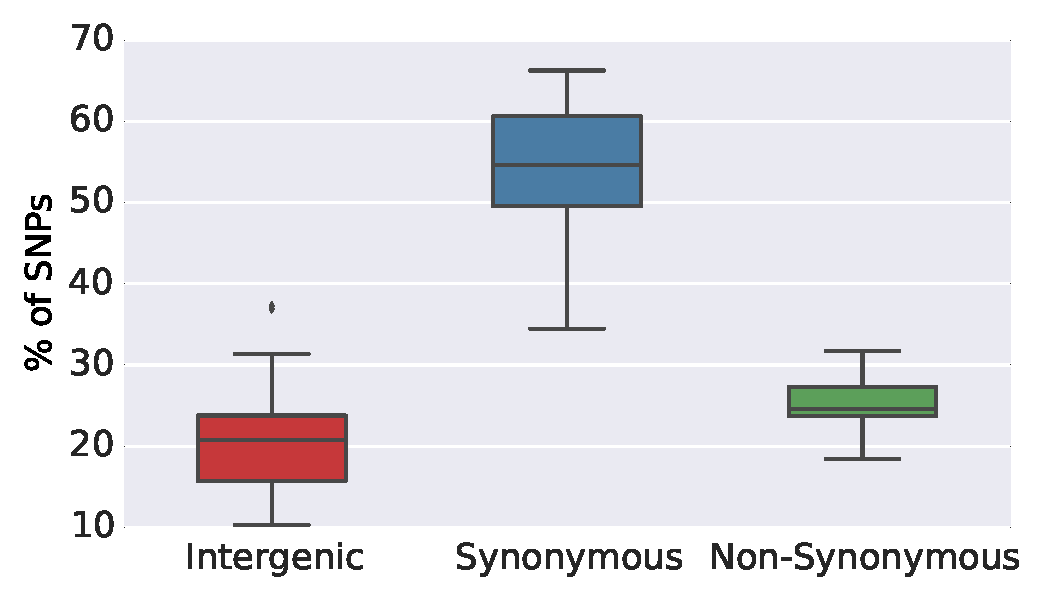
\includegraphics[width=0.7\textwidth,keepaspectratio]{Chapter5/Figures/BoxPlot_TypeofSNPs.pdf}
  \caption{Boxplot summarizing the distribution of type of SNPs (intergenic, synonynous, non-synonymous) for all the genomes and samples.}
  \label{BoxPlotSNP}
\end{figure}

%Figure VENN diagram January
\begin{figure}[!hbtp]
  \centering
  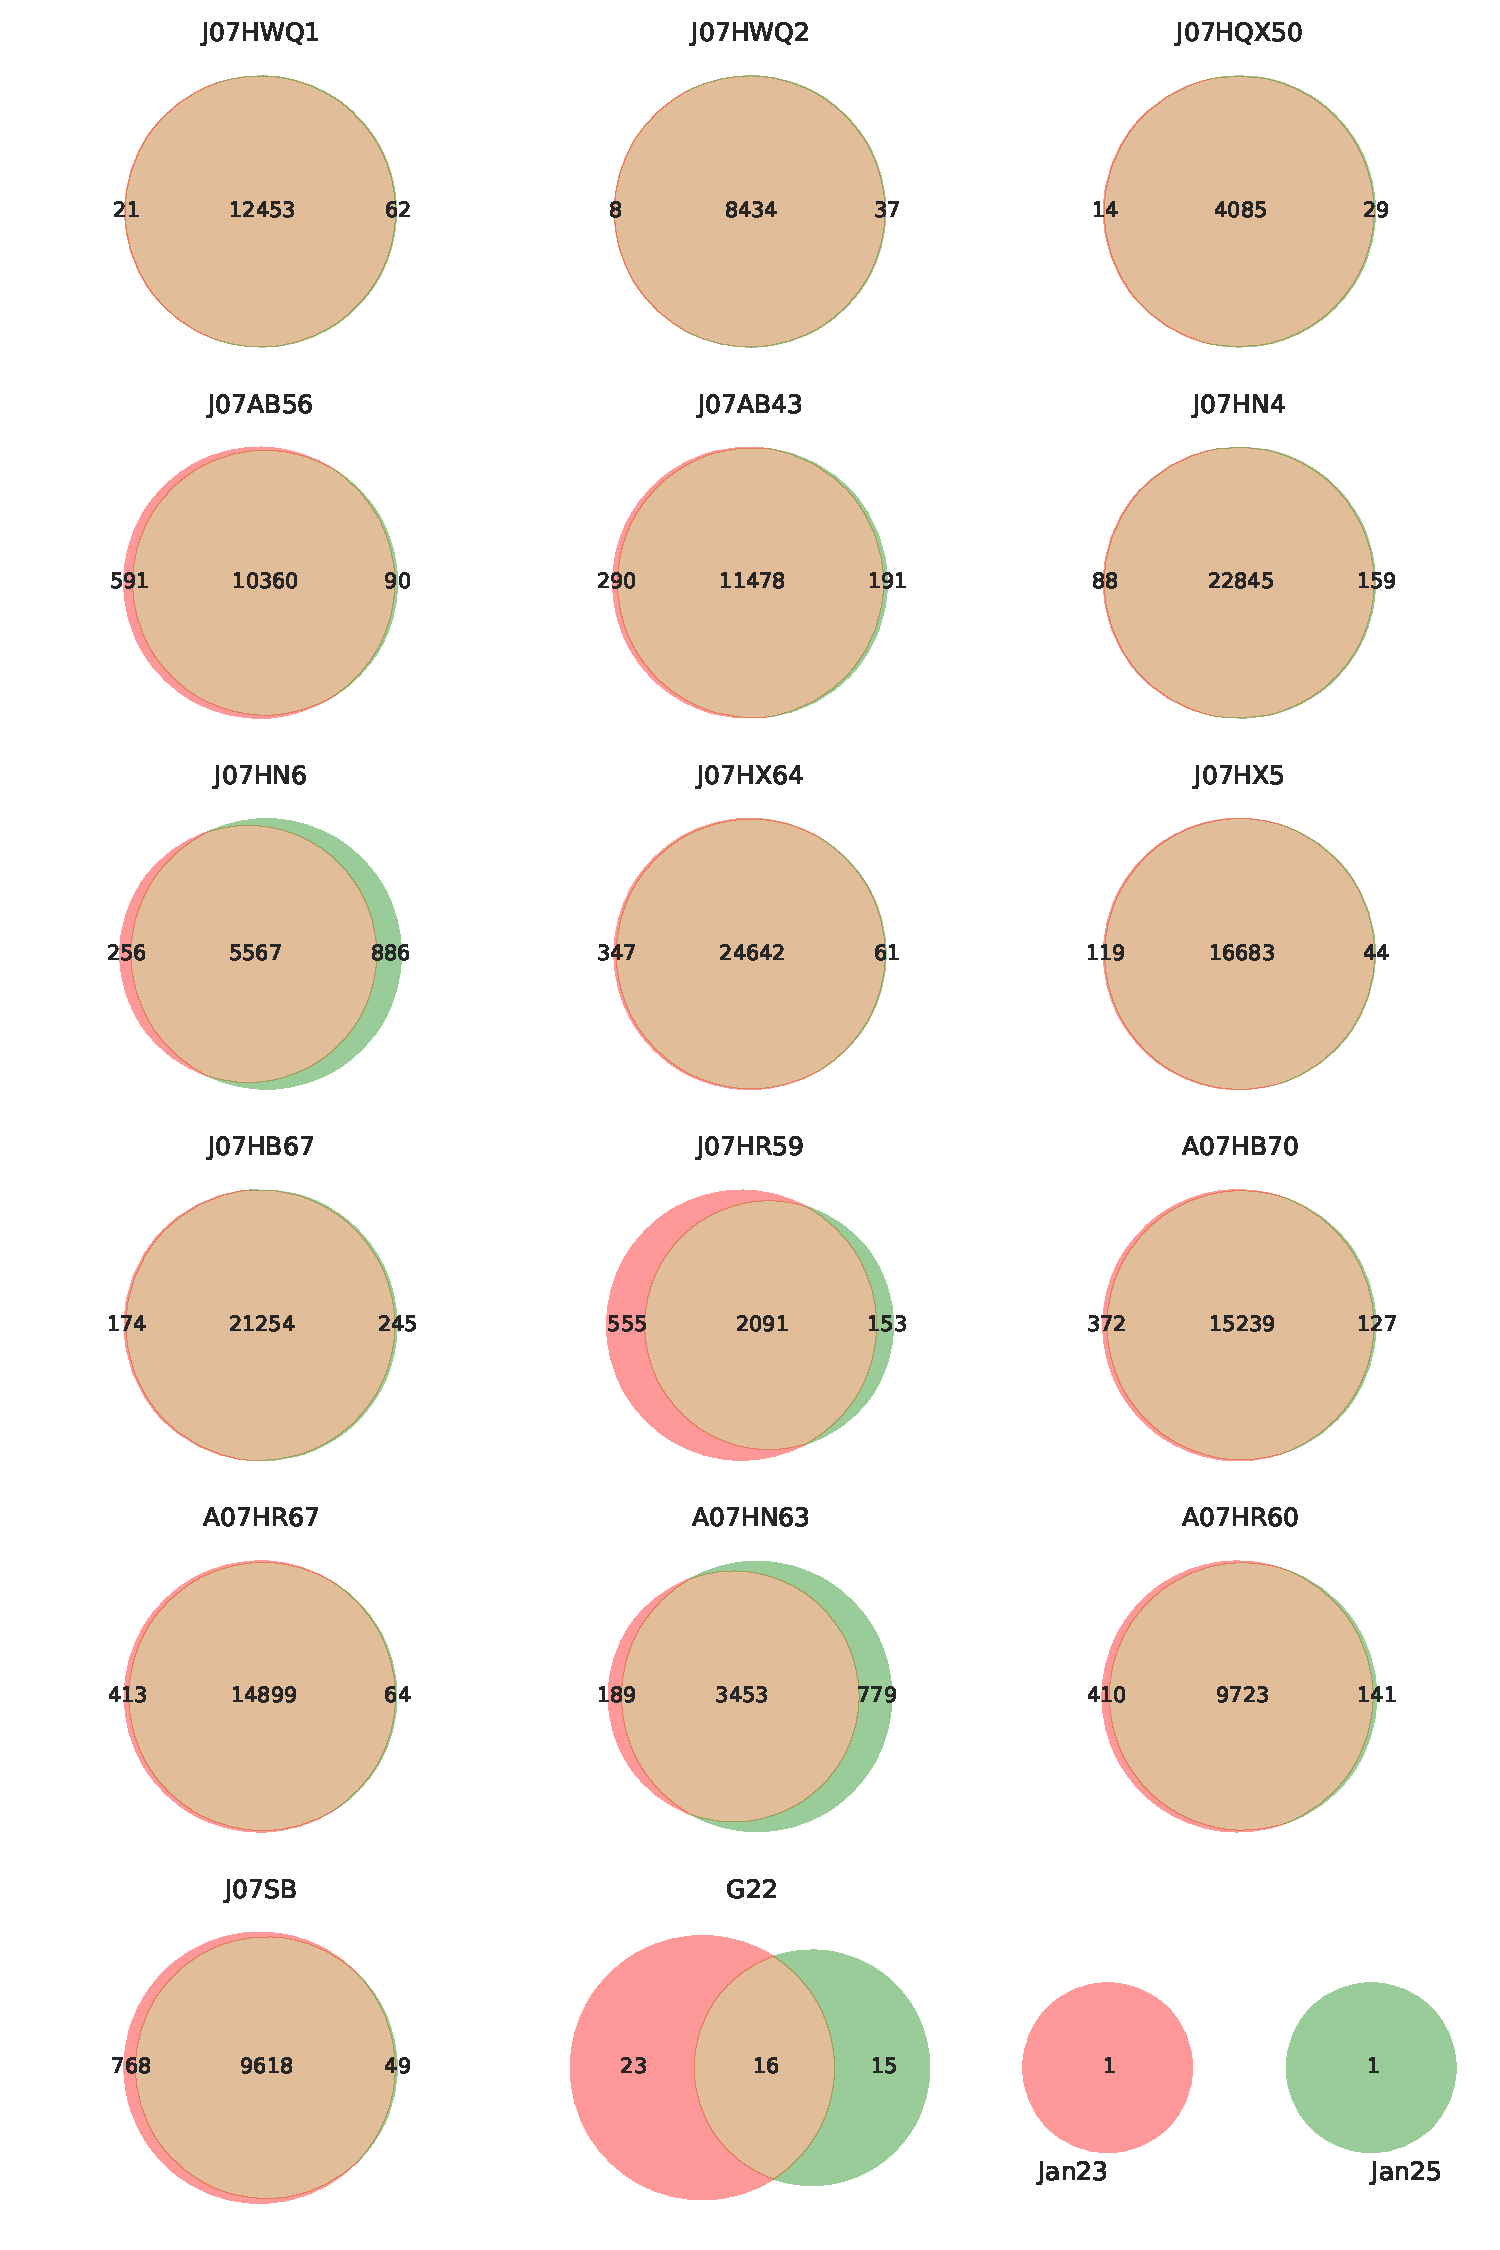
\includegraphics[width=\textwidth,height=0.9\textheight,keepaspectratio]{Chapter5/Figures/Venn_JanuarySNPs.pdf}
  \caption{Venn diagram comparing the SNPs found in the January 23 versus January 25 libraries.}
  \label{VennJan}
\end{figure}

%VENN diagram August
\begin{figure}[!hbtp]
  \centering
  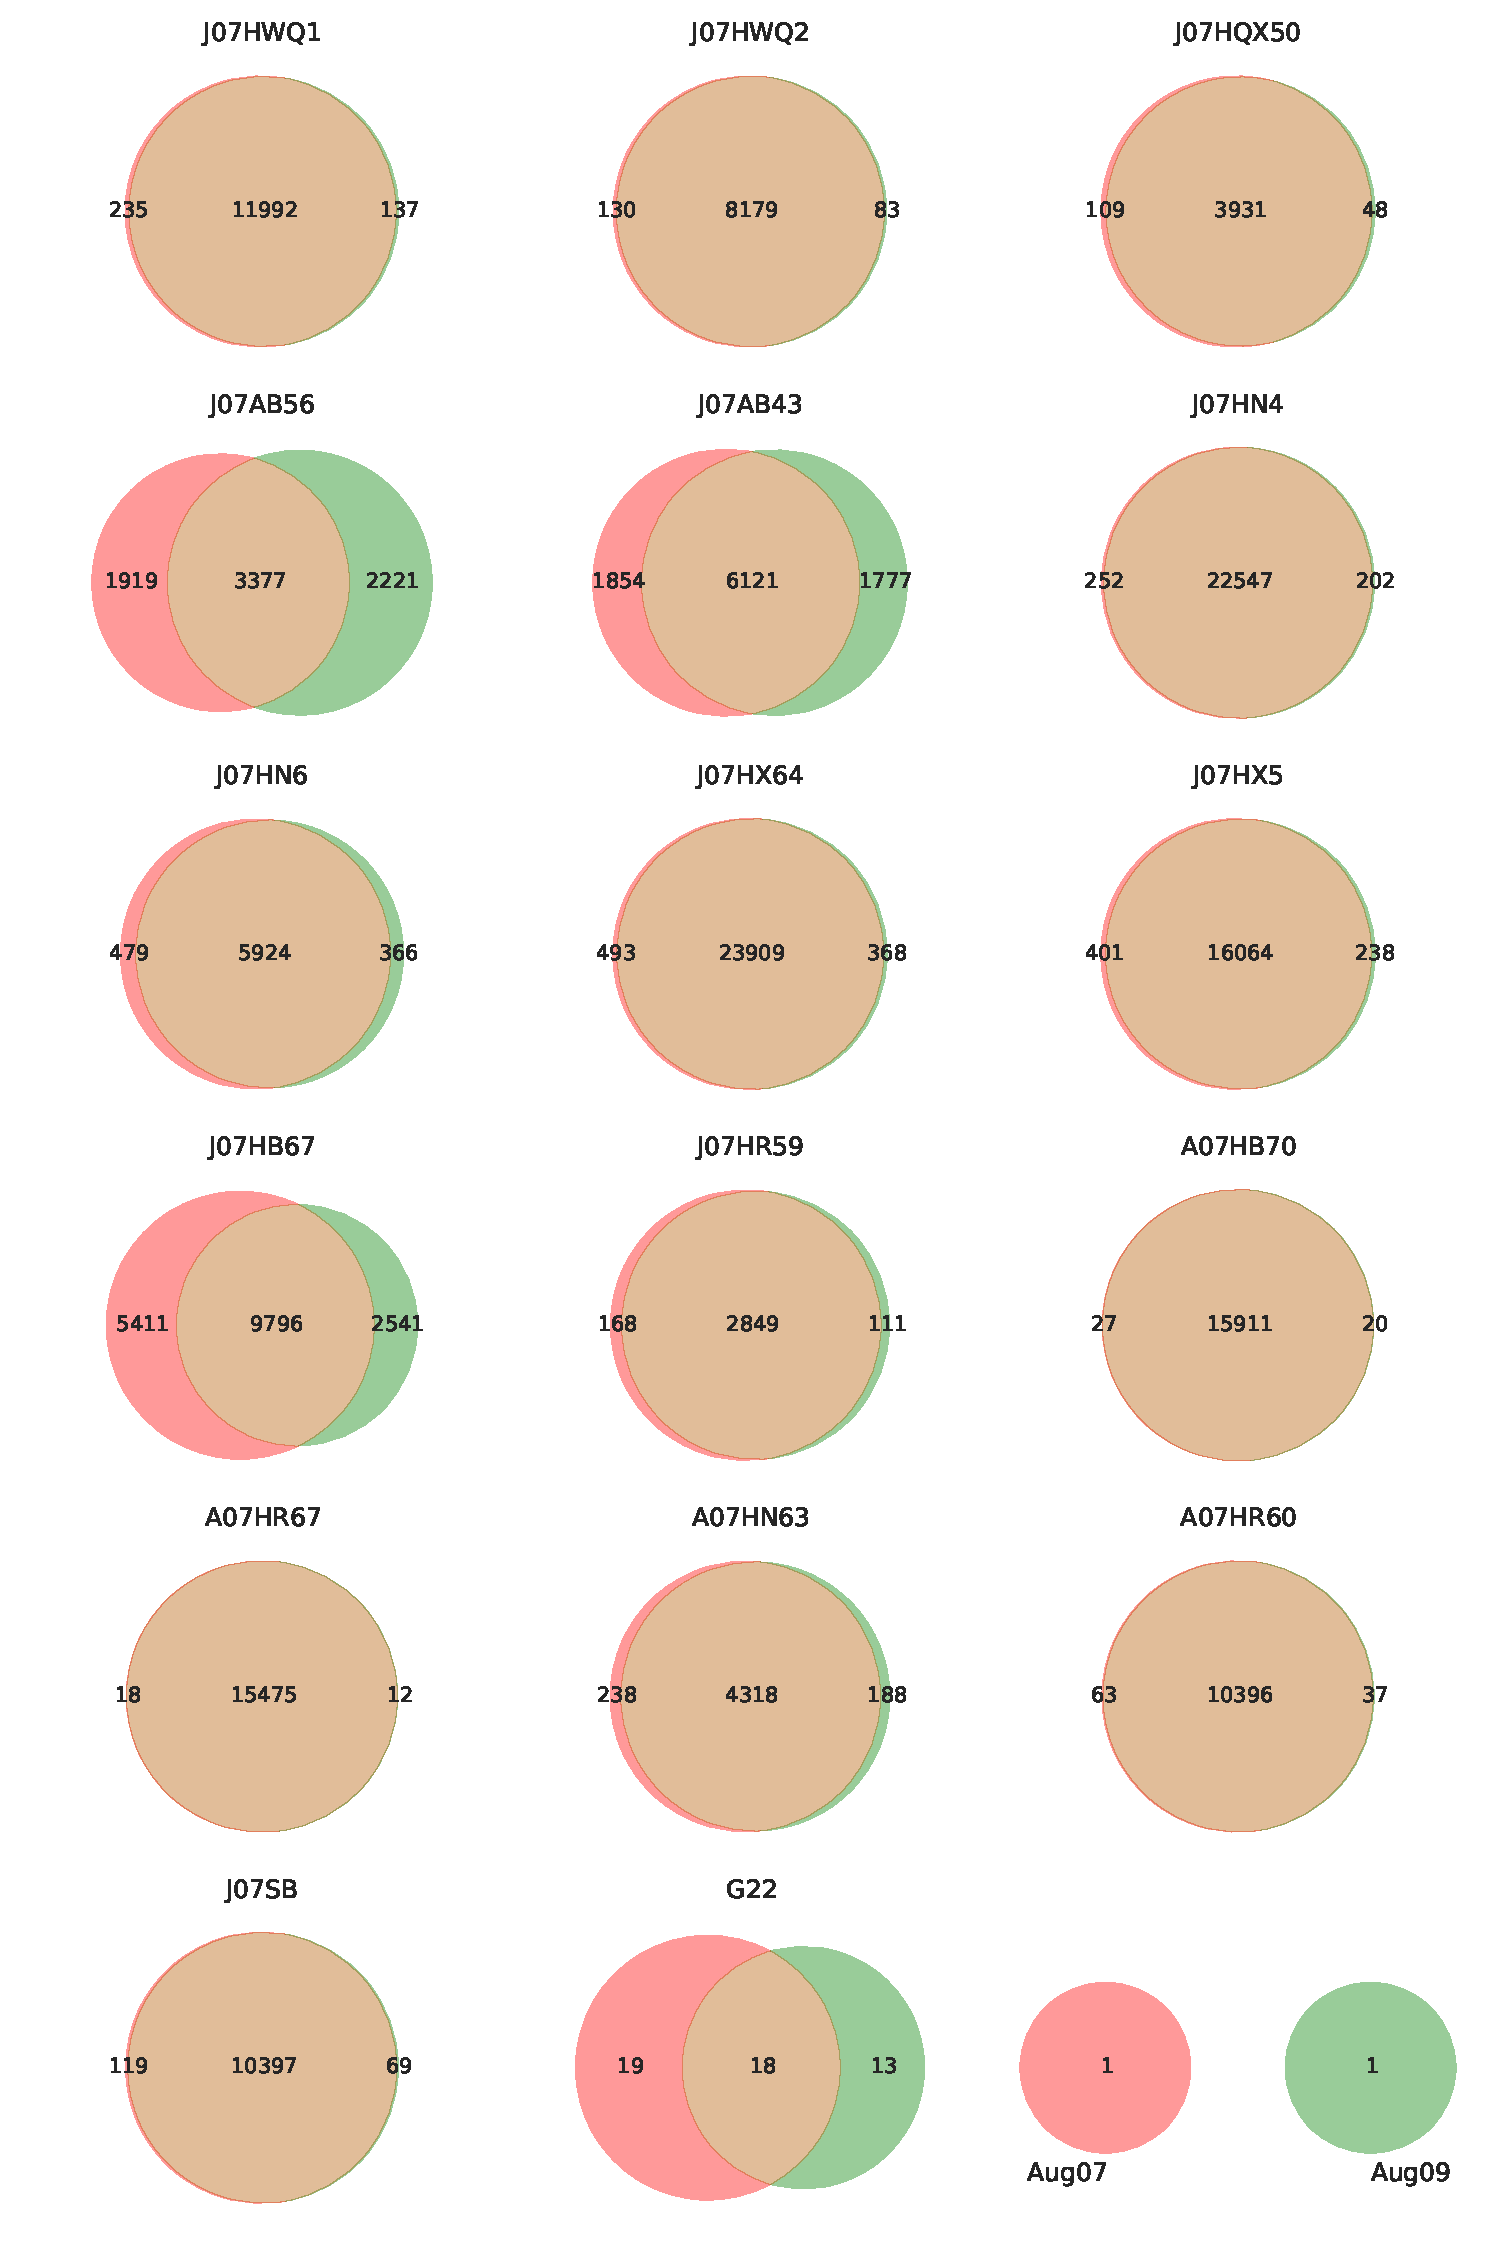
\includegraphics[width=\textwidth,height=0.9\textheight,keepaspectratio]{Chapter5/Figures/Venn_AugustSNPs.pdf}
  \caption{Venn diagram comparing the SNPs found in the August 7 versus August 9 libraries.}
  \label{VennAug}
\end{figure}

%VENN digram both
\begin{figure}[!hbtp]
  \centering
  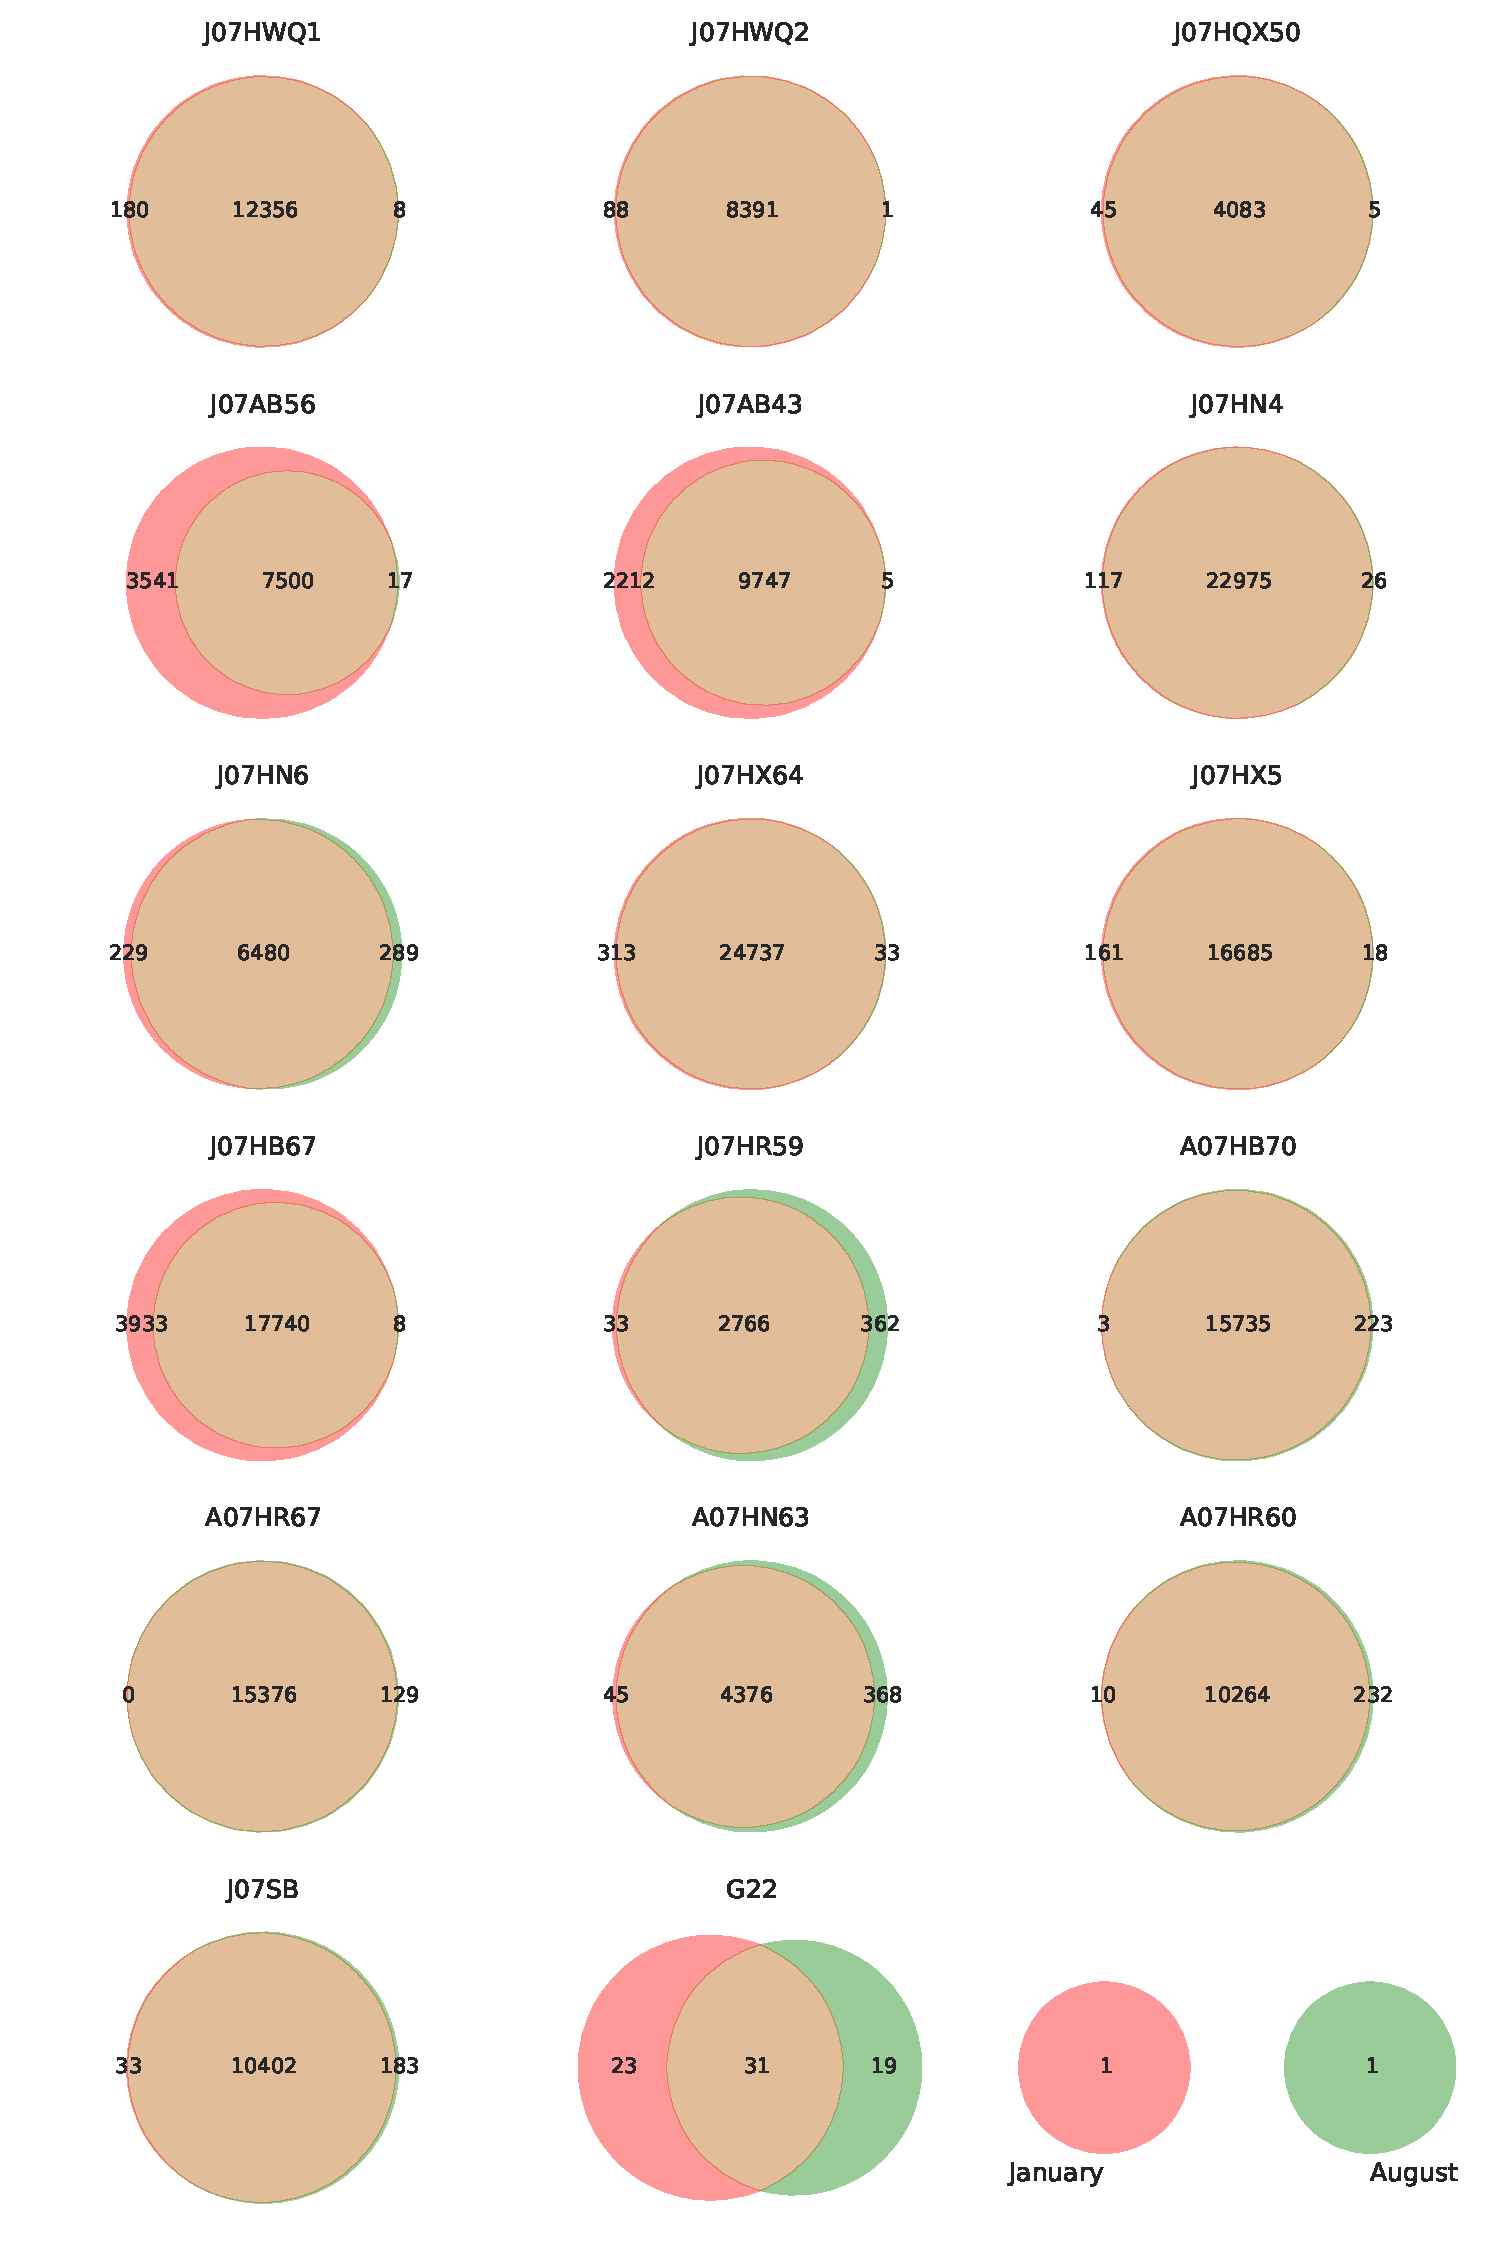
\includegraphics[width=\textwidth,height=0.9\textheight,keepaspectratio]{Chapter5/Figures/Venn_JanAugSNPs.pdf}
  \caption{Venn diagram comparing the SNPs found in the January versus the August libraries}
  \label{VennBoth}
\end{figure}


%%%%%%%%%%%%%%%%%%%%%%%
\clearpage
\subsection{Genes Under Positive Selection}

The results from the variant analyses allow for the evaluation of the role that natural selection is playing in the evolution of individual genes across the community and within individual population. One approach involves looking at the ratio between non-synonymous and synonymous substitution on each individual gene. This is defined as the dN/dS ratio \cite{McDonald:1991hj}, which compares genes between individual species. Similarly, the pN/pS ratio compares this effect at the population level, which is the case here, where we do not have individual isolates that are being under study, but a complex sample \cite{Egea:2008jo,Schloissnig:2012hx}. Using the pN/pS ratio, we can identify genes that are under the effects of positive selection (pN/pS $>$ 1), where natural selection is favoring diversification at the amino acid level \cite{Hurst:2002ht}. On the other extreme, purifying selection (pN/pS $<$ 1) occurs when fewer amino acid changes occur than the ones expected by chance \cite{Hurst:2002ht}.

There are multiple methods for detecting molecular adaptation based on pN/pS ratios \cite{Yang:2000hh}. Because short reads are being used to identify polymorphisms in the genomes, it is not possible to link multiple polymorphisms. This makes statistical approaches, such as Maximum Likelihood and Bayesian methods, difficult to implement for our data \cite{Yang:2000hh}. Instead, a pairwise method was used, quantifying the polymorphisms site by site, using a strategy based on previous work by Tai \textit{et al.} \cite{Tai:2011jo} (Figure \ref{MappingStrategy}). 

\subsubsection{Average pN/pS values for each genome}

First, the average pN/pS values were calculated for each of genomes to determine overall patterns of selection between samples. Figure \ref{Genome_comp_pNpS} shows a comparison of the average pN/pS value for each genome between the months of January and August. Besides the extreme value of G22, no large differences are observed between the two months. This suggests that the overall values of pN/pS for the genes are similar between the two sampling dates.


\subsubsection{pN/pS values and uniquely selected genes}

The pN/pS values were calculated for all the coding regions in each of the reference genomes. To facilitate the comparisons, the analysis was limited to the comparisons between the January and August datasets, merging each individual time point within the same sampling month. An overview of each genome (Appendix \ref{Appendix_pNpS}) shows that there does not appear to be hotspots of selection across the genomes. For example, in the genomes of J07HWQ1 (Figure \ref{example_J07HWQ1_pNpS}) and J07HWQ (Figure \ref{example_J07HWQ2_pNpS}), no striking differences between January and August were observed. Also, the genes under selection are located sparsely along the genome.

Comparing more in detail for January versus August for each reference genome, the results (Table \ref{PSgenes}) indicate that in both samples, the number of genes under positive selection (pN/pS $>$ 1) is similar within each of the reference genomes. Comparing across the genomes, we can see that the percentage of genes under selection in each of the genomes varies between 1.5\% up to 7\% (without considering G22). This is similar to values observed in comparisons for isolate genomes of \textit{Salinibacter} \cite{PeNtildeA:2010ie}, as well in other similar metagenomic studies in \textit{Synechococcus} populations \cite{Tai:2011jo}. A very interesting result, which is similar to what was observed by just looking at the number of shared SNPs between sampling months, is that for several of the genomes, the same genes are under selection in both January and August. Although more formal population analysis needs to be done to confirm this result, this strongly suggests that for some organisms, such as \textit{Haloquadratum} (J07HWQ1, J07HWQ2 and J07HQX50) and \textit{Halonotius} (J07HN4 and J07HN6), among others, the strain variation present in January is similar to that in August. \cite{Vos:2011ux}. For organisms such as the \textit{Nanohaloarchaea} (J07AB56 and J07AB43), the differences suggest the opposite, that there are difference in the strain diversity present in January versus August. By focusing on the genes that are different between sampling months, we can look in more in detail at this variation, providing examples of some of the observed differences.

In the case of J07HWQ1, the single gene that is unique in the August sample codes for a predicted cobalamin biosynthesis protein, based on its COG annotation, and has a von Willebrand factor, type A domain. This protein family has a wide range of functions and, in the case of the J07HWQ1 genome, is located next to predicted ATPase associated diverse cellular activities. The annotation of this protein does not suggest a particular role for the positive selected gene as it may fall into a wide variety of roles, including DNA repair, transcription, ribosomal and membrane transport, and cell adhesion, among other roles \cite{Whittaker:2002ug,Makarova:2010bi}.

For J07HWQ2, the gene that is under positive selection in January codifies for an hypothetical protein that is rich in serine residues. No function is associated with this sequence, but recent evidence from studies in Dictyostelid amoebae, suggest that these domains are frequently present and functional in eukaryote genomes \cite{Tian:2013jv}. In the August sample, the gene showing evidence of positive selection codes for an amino acid transporter.


The other example that will be explored here are the genomes of the \textit{Nanohaloarchaea} (J07AB56 and J07AB43), where we observe differences in the genes that are under positive selection. In J07AB56, the January genes code for hypothetical proteins, transcriptional regulators, and chaperones, among other functions. Interestingly, a large number of proteins related to transmembrane functions was found, including transporters and transmembrane proteins. In contrast, the functions enriched in August, tend to be more hypothetical proteins and some proteins involved in beta-lactamase functions. 

For J07AB43, the differences are hard to pinpoint to specific functional roles as in both cases over 70\% of the functions are annotated as hypothetical proteins. An interesting protein that is under selection in the January sample encodes for a photolyase involved in light-driven DNA repair \cite{Weber:2005fk}. This could be related to the different environmental condition, particularly light intensity and temperature, between the two sampling dates.

\subsubsection{Differences between pN/pS values between sampling dates}

Even when the same genes appeared to be under positive selection for some of the analyzed genomes comparing the January and August samples, even in genes that are under selection in both samples, differences in their pN/pS values (Figure \ref{Gene_pN_pS}) can be observed. In some of the organisms, such as the \textit{Haloquadratum} genomes, only a few genes show different values in one of the samples. On the other hand, in the \textit{Nanohaloarchaea}, there is a broad dispersion of the values, indicating differences in the nucleotide diversity of some of these genes, which could be translated into the presence of multiple strains for these organisms. This also supports the idea that the J07AB43 populations that are present in the January sample are different from the ones present in the August sample \cite{Vos:2011ux}. A similar pattern is observed in the J07HB67 genome and to a lower degree in the A07HN63 genome.


\subsubsection{pN/pS values and functional classification}

One of the limitations of the analysis of pN/pS values is that unless experimental evidence is available for some of the candidate genes, in most of the cases, the associated functions tend to be hypothetical proteins \cite{Tai:2011jo}. At the same time, this is one of the powerful things in the analysis as it can provide candidates for further experimental studies, at least where isolates are available \cite{Fricke:2011gy}.

To narrow some of the functions that could be under selection, the COG (cluster of orthologous groups) functional categories were used. All the genes that had a COG number assigned were analyzed, and COG categories that could be enriched in genes under selection were evaluated by comparing them with the classification of the complete genome (Appendix \ref{Appendix_COGselection}). These results were validated by calculating the odds ratio (the difference between the categories with genes under selection versus the rest of the annotated cogs for the genome), with a one-tailed Fisher exact test (pvalue $<$ 0.05). This analysis provided some functional information on some of the genomes and the genes that are under selection. 

For example, in the case of J07HQX50, the cell wall/membrane/envelope biogenesis category has three genes that are under positive selection. Looking at these genes in more detail, all of them are involved in lipopolysaccharide synthesis, two of them with functions related to the surface layer modification, and the other as a sugar transferase. Considering that these genes are under selection both in January and August, these could suggest that J07HQX50 is under some type of selective pressure to modify its membrane composition, which could be due to multiple factors, including possible phage predation \cite{RodriguezValera:2009cr}.

Another interesting example can be found on J07AB56 (Table \ref{January_COG_Selection_J07AB56}), where in the January sample, the cell motility category is enriched in genes under positive selection. Looking in detail, there are four genes in this group, and all of them are encoding secretion system proteins. Three of them encode for VirB11 components of the type IV secretory pathway, which could play a role in DNA uptake or protein secretion \cite{Chandran:2009fg}. In the August sample, a different category is enriched, intracellular trafficking, secretion, and vesicular transport, but a detailed look of the genes, shows that most of them encode for type IV secretory systems or protein export component, suggesting a similar role as in the January case, where the genes involved in protein secretion are under positive selection. It has been observed in some Bacteria that secreted proteins have rapid evolution rates \cite{Nogueira:2012gv}, and some of these proteins could be involved with interaction with the outside environment, as they could be attached to the cell wall and include functions such as protection against grazing \cite{Matz:2005ik} and/or competition against other microbial groups \cite{Kirkup:2004hj}.


%Figure Mapping
\begin{figure}[!hbtp]
  \centering
  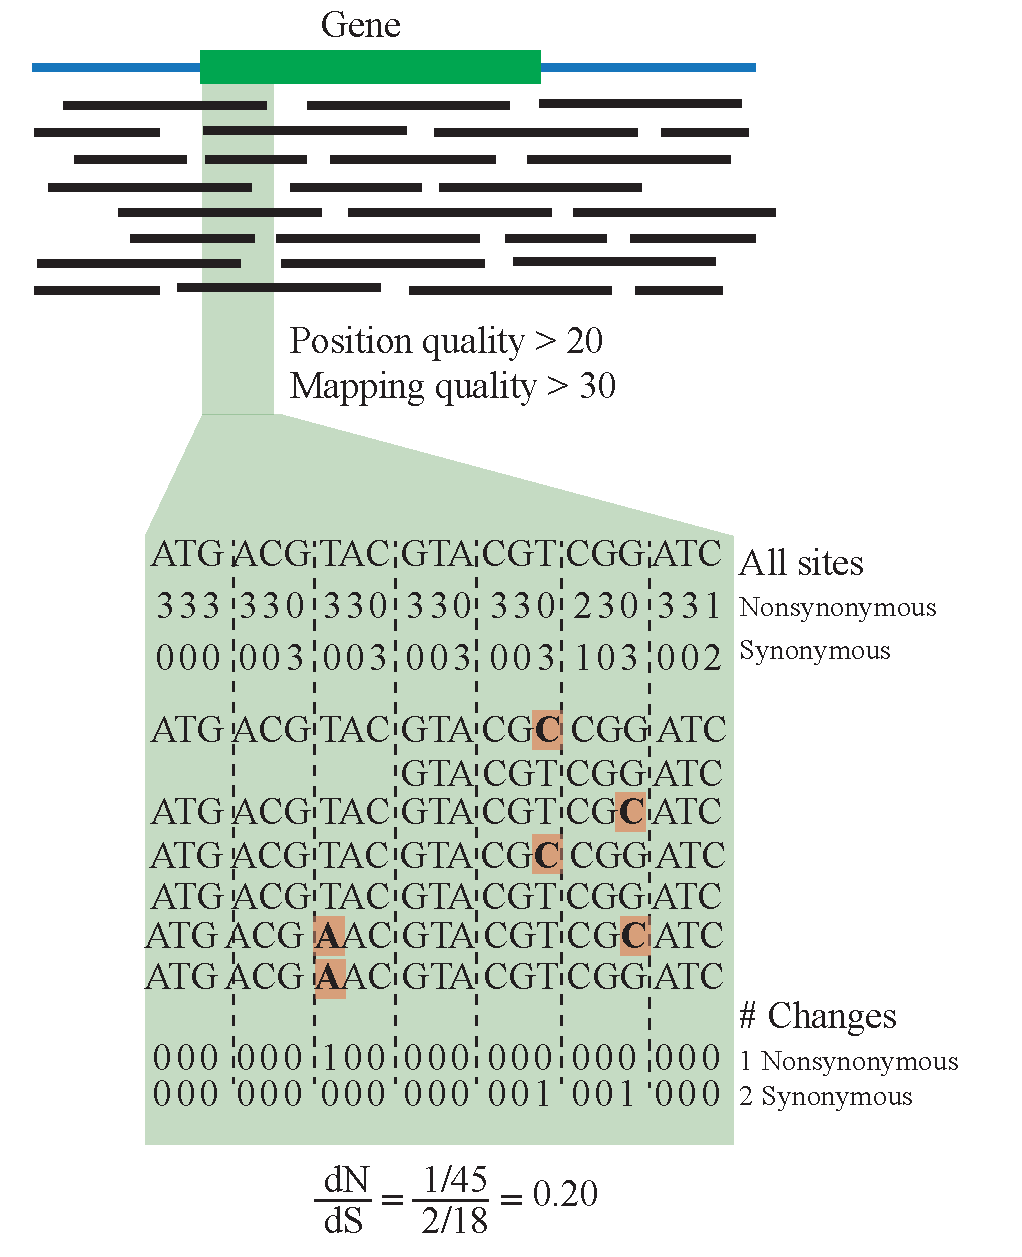
\includegraphics[width=0.7\textwidth]{Chapter5/Figures/MappingStrategy.pdf}
  \caption{Overview of the strategy used to quantify the SNPs differences on each gene, and calculate the ratio of non-synonymous to synonymous substitutions (pN/pS) on each of the reference genome. Figure based on \cite{Tai:2011jo}.}
  \label{MappingStrategy}
\end{figure}

%Table Genes positive selection
\begin{table}[hbt]
  \caption{Count of Genes under positive selection (pN/pS $>$ 1). Data where pS/pS = 0/0 or pS = 0, was not included.}
  \begin{tabularx}{\textwidth}{L{2.2cm}R{2cm}R{3cm}R{3.2cm}R{2cm}}
  \hline
    \textbf{Genome} & \textbf{CDS} & \textbf{January} & \textbf{August} & \textbf{Unique (Jan/Aug)} \\
    \hline
     \textit{J07HWQ1} & 3,584 & 61 (1.7) & 62 (1.7) & 0/1 \\
     \textit{J07HWQ2} & 3,856 & 46 (1.2) & 46 (1.19) & 1/1 \\
     \textit{J07HQX50} & 2,872 & 19 (0.7) & 19 (0.7) & 0/0 \\
     \textit{J07AB56} & 1,411 & 96 (6.8) & 79 (5.6) & 37/20 \\
     \textit{J07AB43} & 1,678 & 96 (5.7) & 87 (5.2) & 25/16 \\
     \textit{J07HN4} & 3,230 & 198 (6.1) & 196 (6.1) & 3/1\\
     \textit{J07HN6} & 2,914 & 59 (2.1) & 64 (2.2) & 3/8 \\
     \textit{J07HX64} & 3049 & 191 (6.2) & 189 (6.2) & 3/1 \\
     \textit{J07HX5} & 2,139 & 137 (6.4) & 137 (6.4) & 1/1 \\
     \textit{J07HB67} & 2,847 & 196 (6.8) & 168 (5.9) & 54/26 \\
     \textit{J07HR59} & 1,841 & 27 (1.4) & 33 (1.8) & 0/6 \\
     \textit{A07HB70} & 2,514 & 154 (6.1) & 156 (6.2) & 1/3 \\
     \textit{A07HR67} & 2,891 & 167 (5.8) & 171 (5.9) & 0/4 \\
     \textit{A07HN63} & 2,507 & 42 (1.7) & 50 (2.0) & 4/12 \\
     \textit{A07HR60} & 2,861 & 83 (2.9) & 87 (3.1) & 2/6 \\
     \textit{G22} & 3,525 & 0 (0) & 0 (0) & 1/1 \\
     \textit{J07SB} & 1,641 & 91 (5.6) & 91 (5.5) & 2/2\\     
  \end{tabularx}
  \label{PSgenes}
\end{table}

%Figure COG pNpS average
\begin{figure}[]
  \centering
  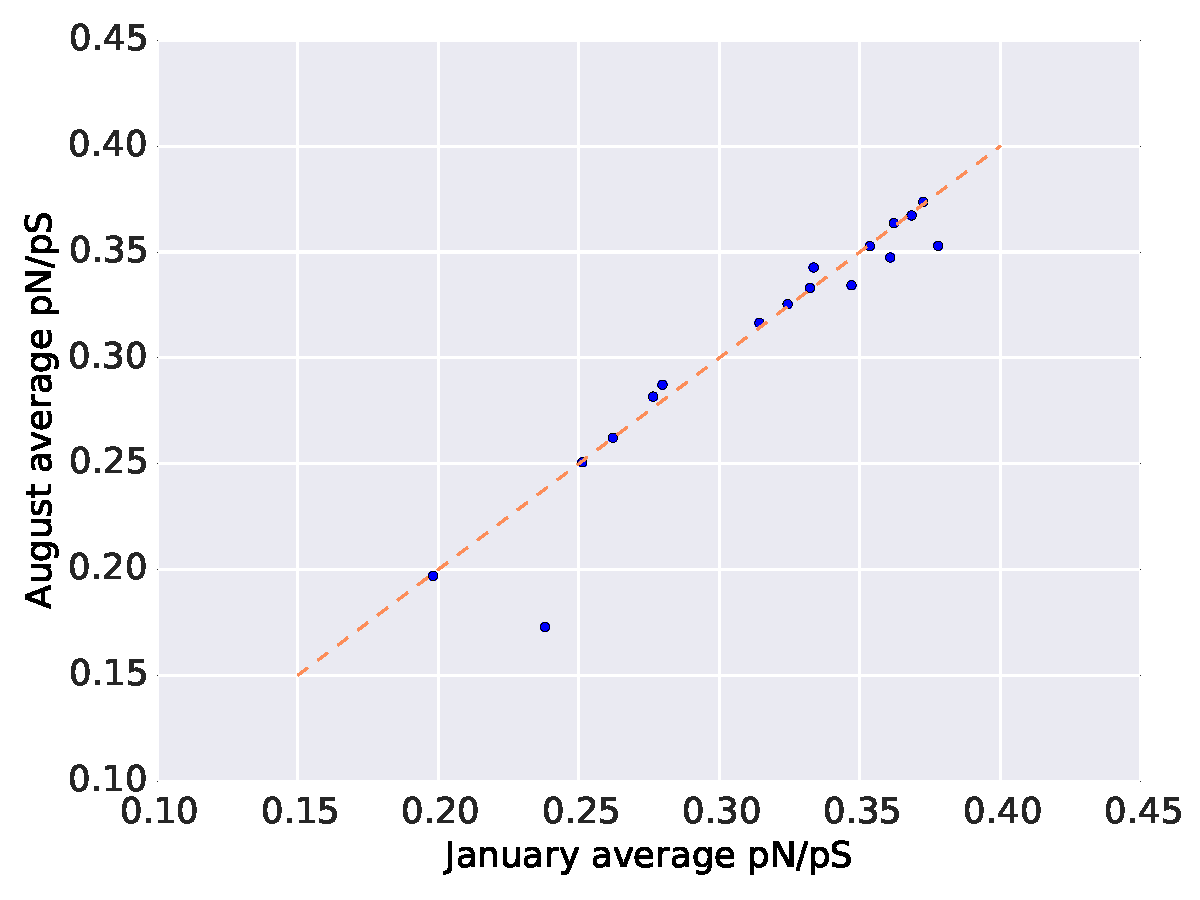
\includegraphics[width=0.75\textwidth,height=\textheight,keepaspectratio]{Chapter5/Figures/Scatter_Genomes_pNpS.pdf}
  \caption{Scatterplot of average pN/pS ratios in January versus August, for each of the reference genomes used in the analysis. The extreme value in the right bottom of the plot, corresponds to G22.}
  \label{Genome_comp_pNpS}
\end{figure}


%Figure COG pNpS average
\begin{figure}[]
  \centering
  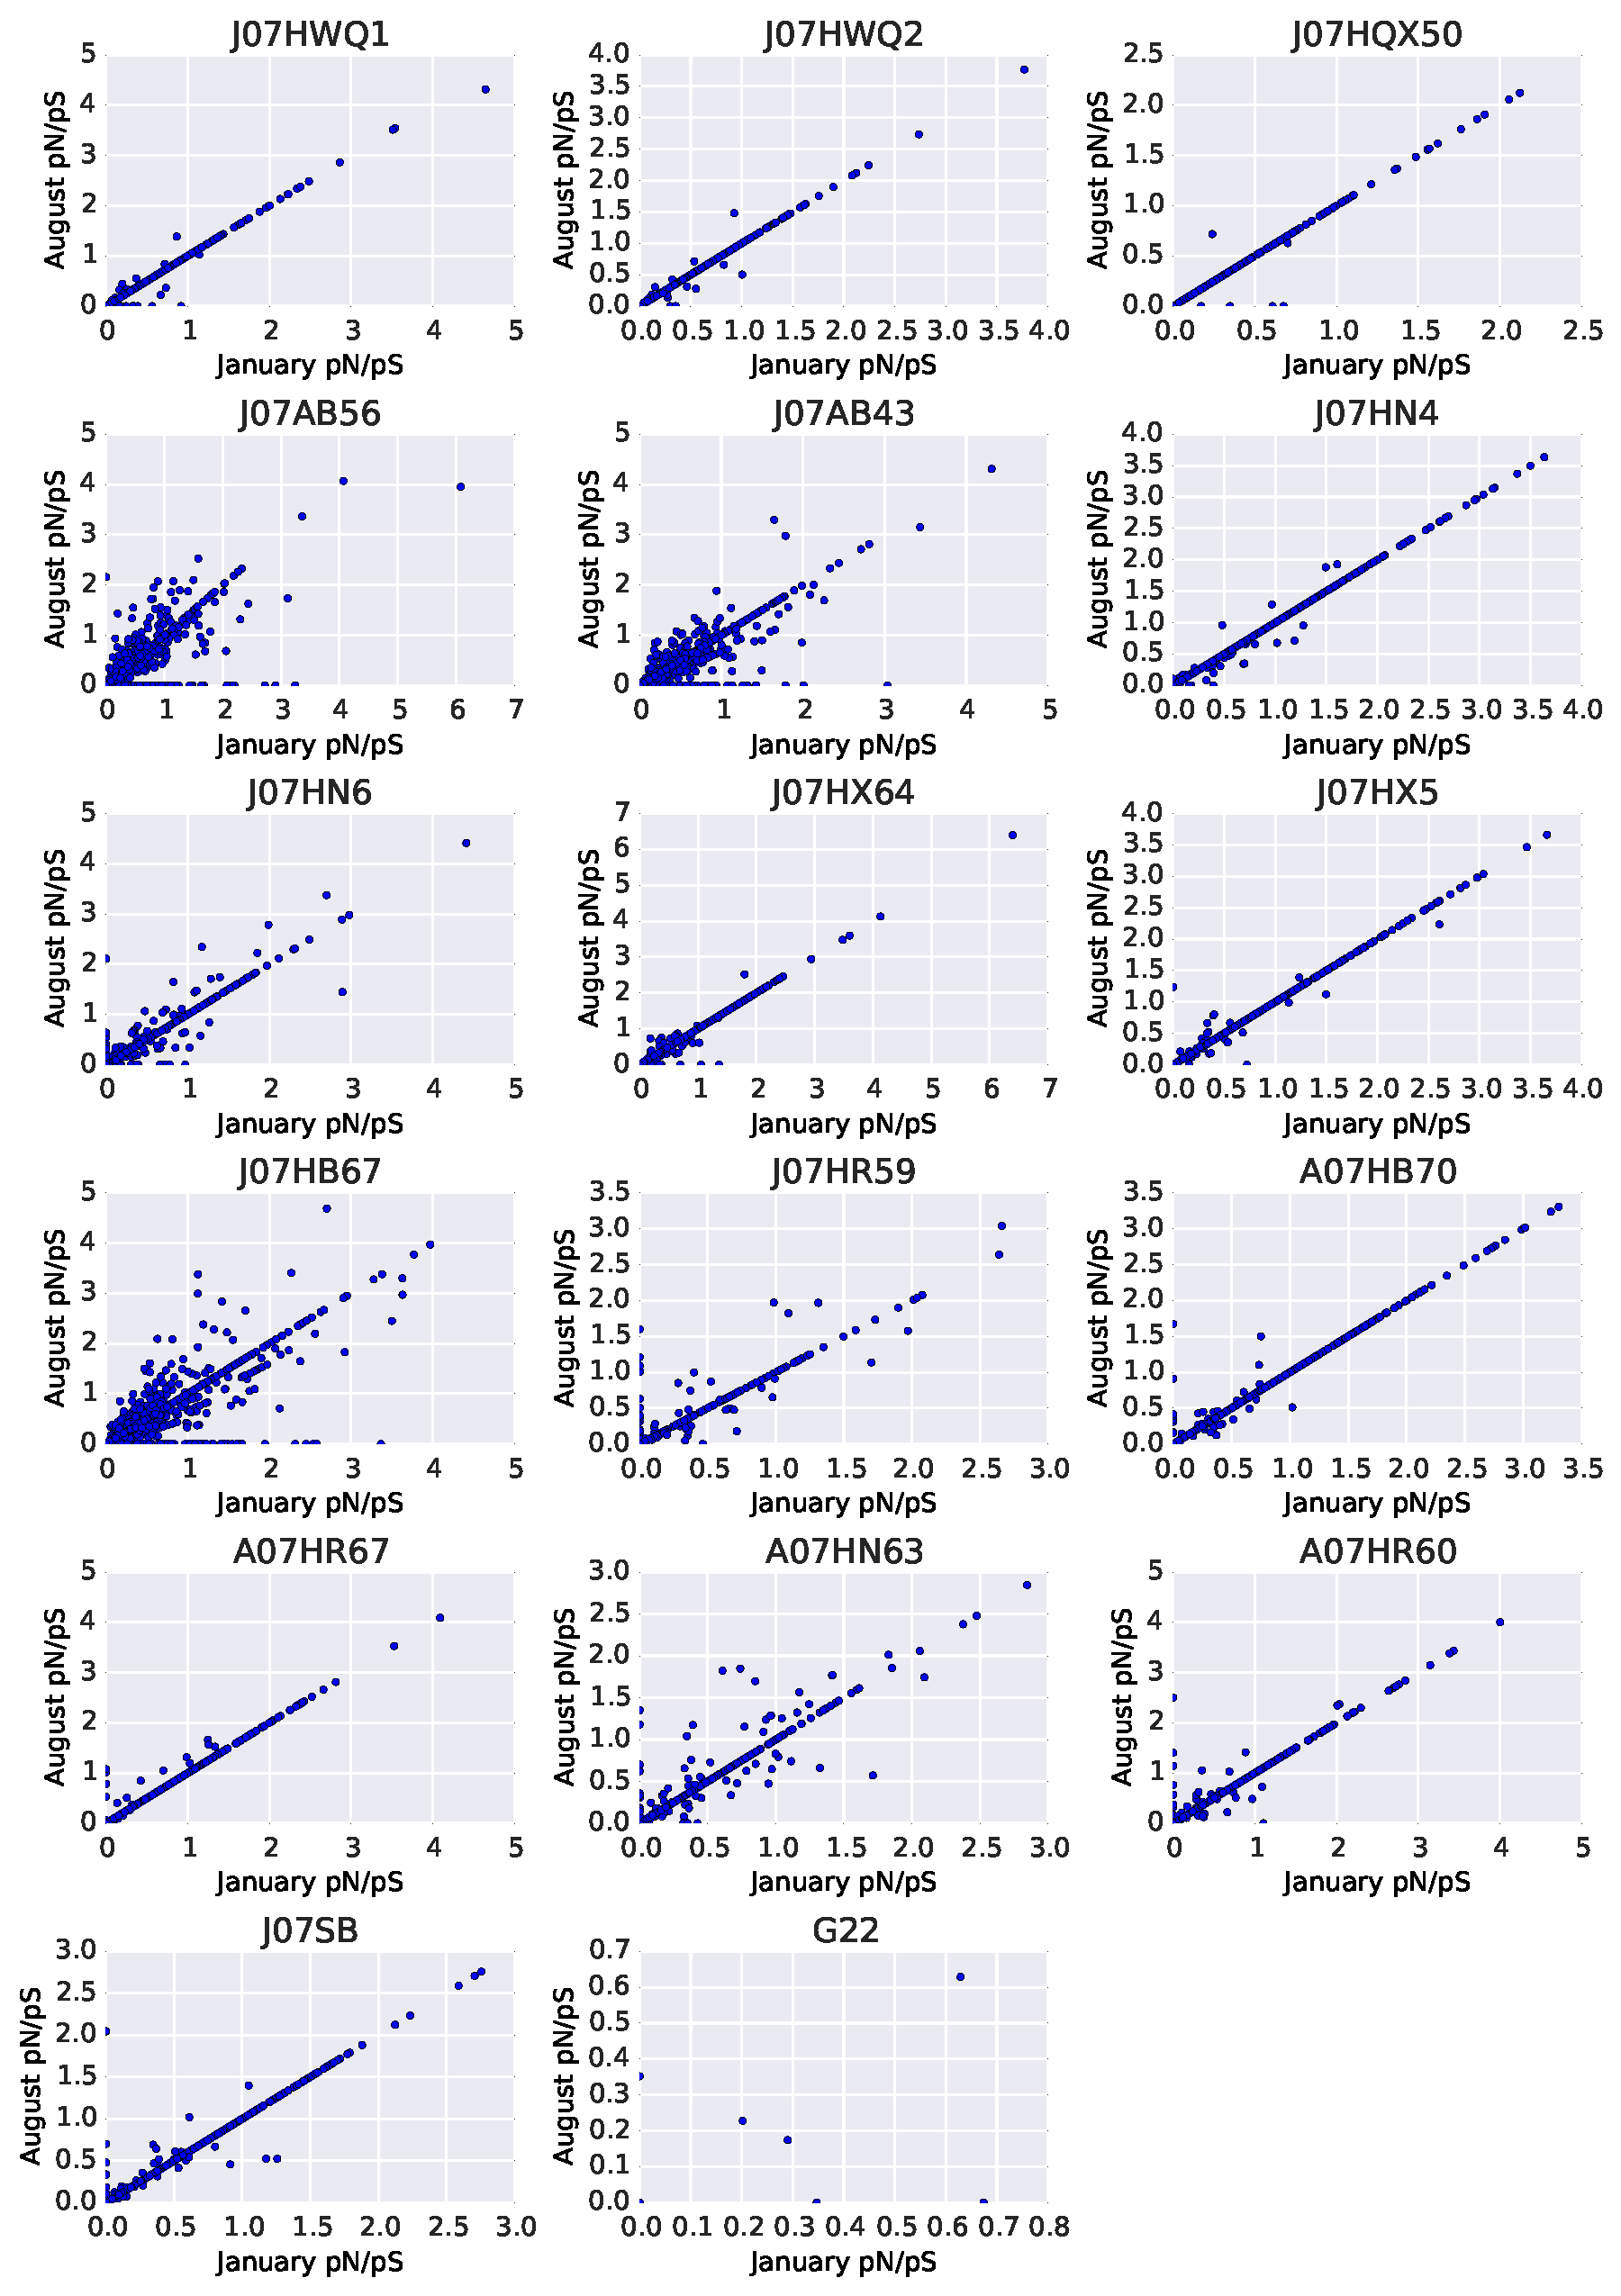
\includegraphics[width=\textwidth,height=0.8\textheight,keepaspectratio]{Chapter5/Figures/Gene_pN_pS.pdf}
  \caption{Scatterplot of the pN/pS values for each of the reference genomes, comparing the pN/pS values in January versus August.}
  \label{Gene_pN_pS}
\end{figure}

%Figures pn/ps along genome
\begin{figure}[p]
  \centering
  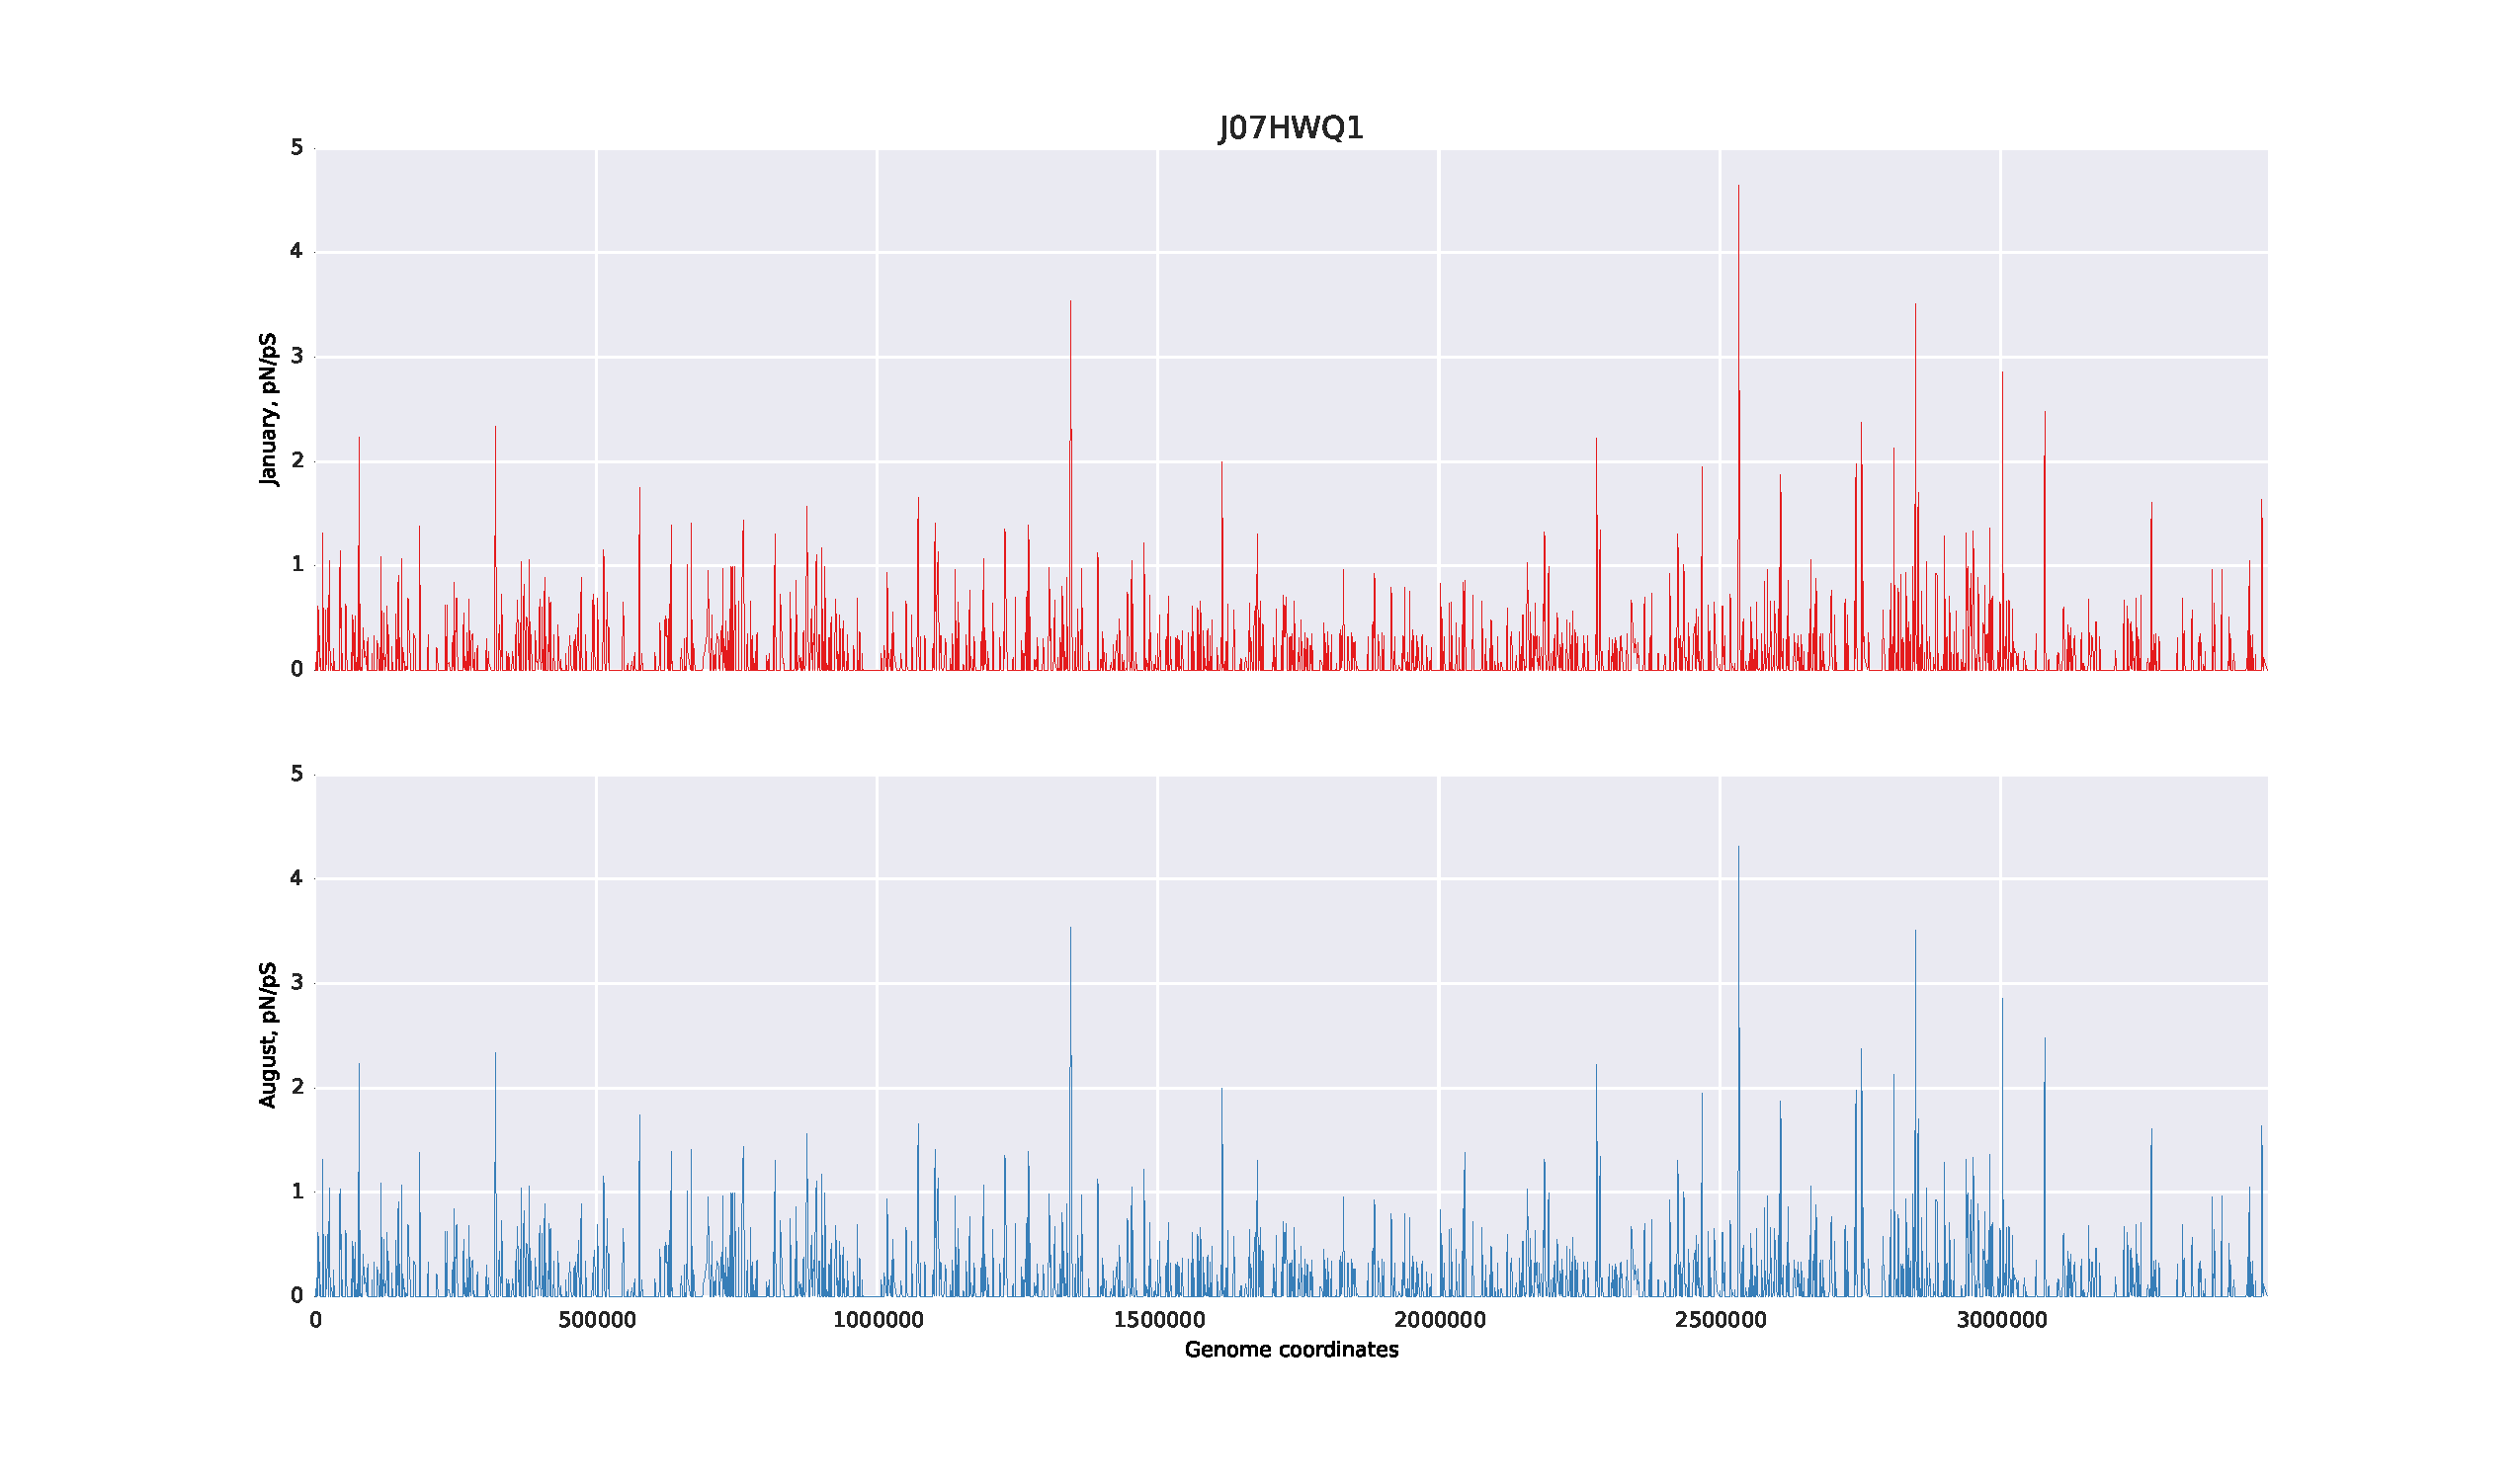
\includegraphics[width=\textwidth,height=\textheight,keepaspectratio]{Chapter5/Figures/pn_ps_plots/J07HWQ1_pNpS_density.pdf}
  \caption{pN/pS values for each gene in the J07HWQ1 genome. Top panel shows the values using the reads from the January samples. Bottom panel shows the values using the reads from the August sample.}
  \label{example_J07HWQ1_pNpS}
\end{figure}

\begin{figure}[p]
  \centering
  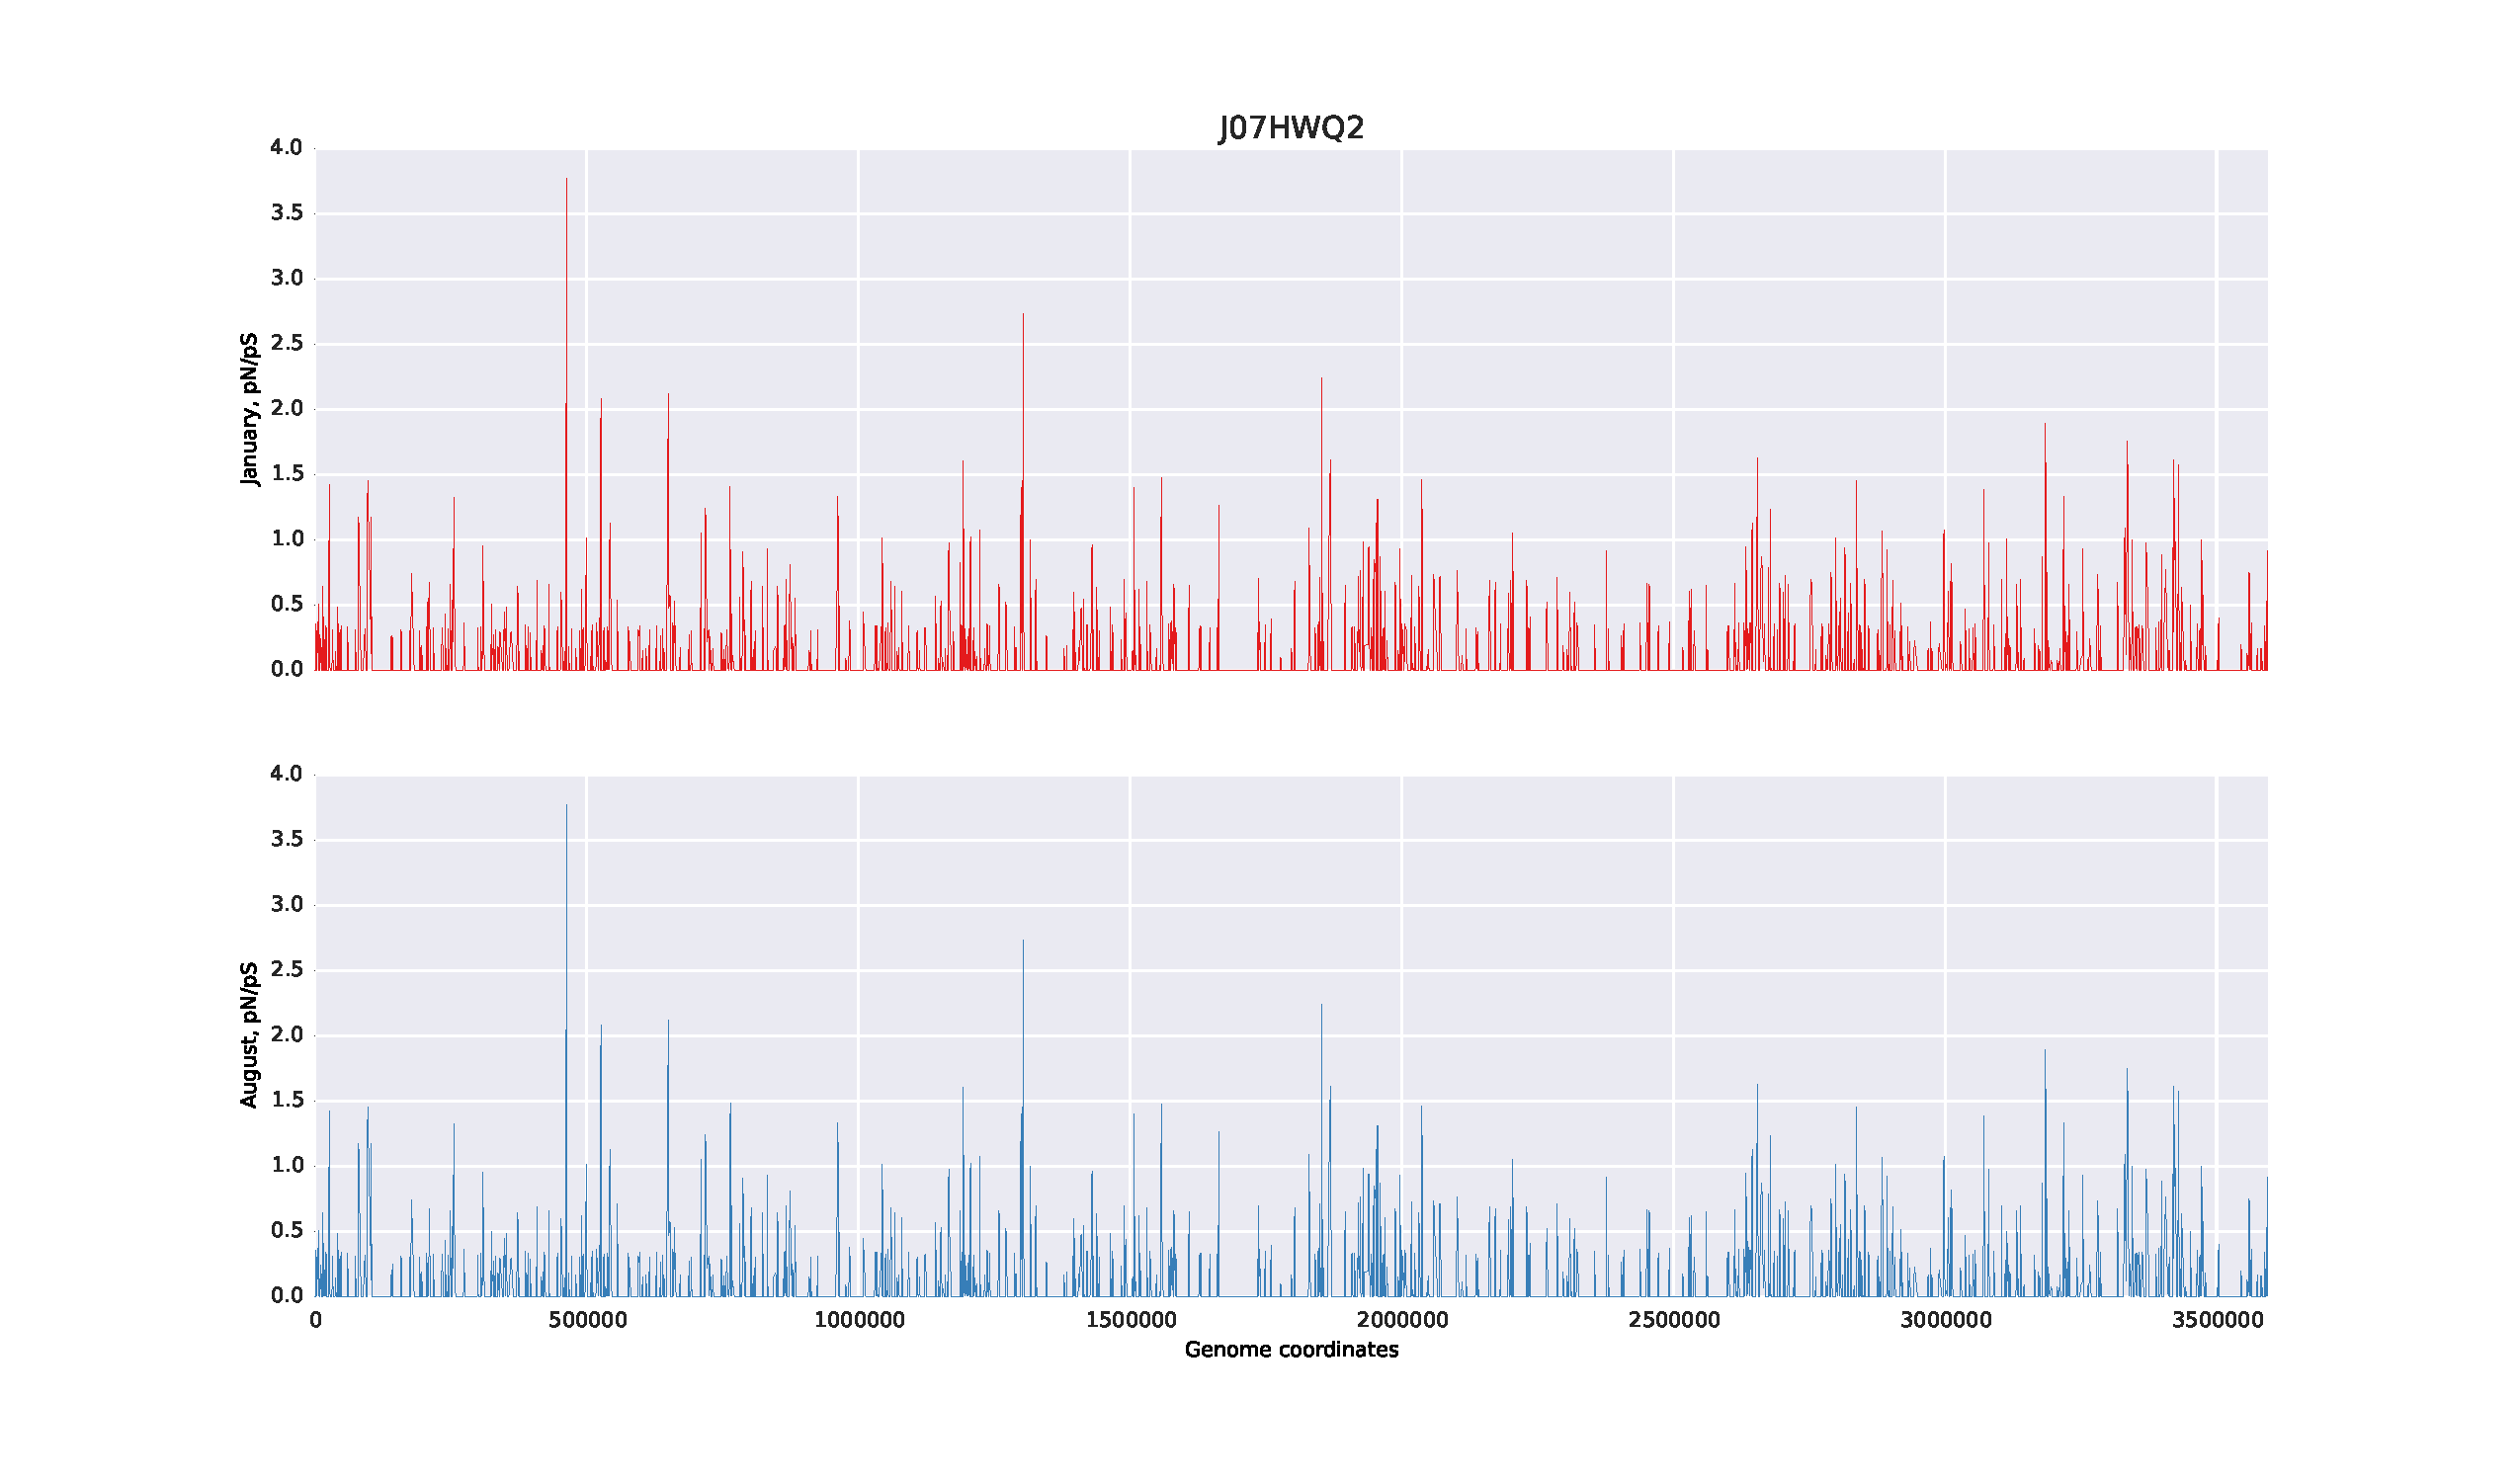
\includegraphics[width=\textwidth,height=\textheight,keepaspectratio]{Chapter5/Figures/pn_ps_plots/J07HWQ2_pNpS_density.pdf}
  \caption{pN/pS values for each gene in the J07HWQ2 genome. Top panel shows the values using the reads from the January samples. Bottom panel shows the values using the reads from the August sample.}
  \label{example_J07HWQ2_pNpS}
\end{figure}


\clearpage
\section{General Discussion}

The main goal in this chapter was to provide a big-picture analysis of the relative abundance and fine-scale genetic diversity that is present in the Lake Tyrrell microbial community. The resulting data shows that the combination of high-throughput data with habitat-specific genomes assembled from metagenomic datasets from the same environment \cite{Narasingarao:2012kp,Podell:2013kx,Podell:2013fp} provides an opportunity to evaluate the relative abundance of the members of the microbial community and allows the exploration of the genetic diversity that exists in the population.

One of the limitations of the current approach is the stringent parameters used in the analysis. Depending on the goal in mind, these parameters should be evaluated. A clear example of this is that during the analysis the G22 genome usually recruited a low number of reads (its coverage was no larger than 1.2X). This also highlights the issue of isolates and their real abundance in natural microbial communities. G22 was isolated from water samples collected in August of 2007 and chosen for genome sequencing based on similarities with the A07HB70 genome \cite{Ugalde:2013hb}. Based on the results presented here, it seems that not only  is this a different species (maybe even more distant) than A07HB70, but also that its abundance in the Lake Tyrrell community is low.

Another element that needs to be taken in consideration is the viral component of the community. Recently, several assembled viral genomes from members of this community were described \cite{Emerson:2012gh,Emerson:2013ck}. Although the filtering strategy (direct water into a Sterivex) did not enrich for viruses (although large viruses could have been retained), using these genomes will allow us to evaluate the relative abundance of the viruses within the sequence dataset and provide an overview of the fine-scale genetic diversity that could be present on these phage genomes. It is possible that the low variation between the January and August samples, which was observed in the archaeal and bacterial genomes, is different in viral populations, as it has been suggested in other hypersaline ecosystems \cite{RodriguezBrito:2010in}.

One of the most interesting results is the possibility that some of the populations that are present in the January community are the same that are present in August, such as the \textit{Haloquadratum} groups, and what it changes over time is the relative abundance of the genomes. To validate these observations, a more detailed population analysis needs to be performed \cite{Schloissnig:2012hx,Kryazhimskiy:2008hq,Whitaker:2006gf}, including detailed population metrics such as nucleotide diversity within and between populations.

A large percentage of the genes found to be under positive selection were hypothetical proteins, similar to what has been observed in similar studies \cite{Tai:2011jo,Hemme:2010ds}. The potential of this type of analysis, both in isolate genomes and metagenomes, is that it provides a list of candidate genes for study with the idea that even if the candidate is a hypothetical protein, the evidence that is under selection can be used to prioritize it for further studies. Along this line, future work will include a more detailed analysis of each of the genes, including hypothetical proteins. For example, the incorporation of structure modelling may provide some additional information by mapping those sites that are under selection to the three-dimensional structure of the protein. In addition, this list can constitute possible markers to look for in further metagenomic surveys of this community.

One element that was not incorporated in the current analysis is the role of horizontal gene transfer and its relationship to natural selection \cite{Wiedenbeck:2011ena}. It has been suggested that horizontally transferred genes evolve faster than duplicated genes in Bacteria \cite{Treangen:2011ca}. This suggests that some of the genes that were under positive selection could have been acquired from other organisms.

Moving from away from the broad comparison, the attention can also be focused on individual species groups. One of the best candidates for this analysis is \textit{Haloquadratum}. Besides the two genomes assembled from the Lake Tyrrell community, there are two genome sequences from isolates that are publicly available \cite{Bolhuis:2006gm,DyallSmith:2011tu}. A pan-genome analysis of the four genomes could help to explain some of the results for the positive selected genes. For example, it has been suggested that core genes have lower rates of selection compared to non-core genes \cite{Jordan:2002by,RodriguezValera:2012cg}.

Finally, most of the effort was focused on the study of the positively selected genes as the results provide a small dataset to focus on. However, also looking at those genes under purifying selection could provide interesting information about the organisms. It should be expected that housekeeping genes will be under purifying selection as any changes could lead to lethal mutations for the organisms \cite{Palenik:2009kx,Schloissnig:2012hx}. Also, in \textit{Eschericha coli}, it has been shown that synonymous mutations alter the rates of gene expression, so it is not only the role of natural selection on changing the amino acid sequence of a protein, but also on how it affects the expression of the gene.

\section{Conclusions}

The results presented in this chapter provide the preliminary framework of analysis to quantify and evaluate the relative abundance and fine-scale genetic variation that is present in natural microbial communities. The genes and functions identified in this chapter as being under positive selection can be used in the future as markers for the study of microbial communities, particularly for future work in the Lake Tyrrell ecosystem.

The methods and results described here represent one of the few studies where habitat-specific genomes are used to quantify the genetic diversity present in a community. This work provides the first overview of this genetic diversity, generating the necessary data that will be required for further detailed analysis. In addition, the methods developed here can be applied to other microbial communities and are not limited to the study of the Lake Tyrrell hypersaline community.

\section{Acknowledgments}
I would like to thank Sheila Podell for discussions on the analysis and ideas for this Chapter. Also, funding from Fulbright-Conicyt and NSF 1149552 is acknowledged, and to Amazon Web Services for an education grant that allowed the use of the EC2 infrastructure.


%%%%%%%%%%%%%%%%%%%%%%%


%\todo{Modify reference SNPs section}
%\subsection{Genome information and reference SNPs}
%To generate a list of reference SNPs,  11 archaeal genomes obtained from the assembly of the metagenomic samples were analyzed. The results (Table \ref{GenomeTable}), shows the total number of SNPs identified in each of the genomes. Although the low depth of the analysis does not allow to make any assumptions about the levels of genetic heterogeneity present on each population, still can provide a valid picture that can be contrasted with the Illumina data. Figure \ref{ReferenceSNPsType}, shows a comparison of the location and type of variation found among the genomes. Most of the identified polymorphisms are synonymous, meaning that they do not produce any changes in the amino acid sequence. Comparing among the populations, most of the polymorphisms fall into coding regions, with some extreme cases such as in \textit{Nanosalina} sp. J07AB43 and \textit{Nanosalinarum} sp. J07AB56, where only 5\% and 8\%, respectively, of the polymorpshism are found in intergenic regions. This reflects the streamlined nature of these genomes, and their reduced intergenic space \cite{Narasingarao:2012kp}. An interesting situation occurs in the case of \textit{Nanosalina} sp. J07AB43, which has a high number of polymorphisms classified as other (mostly frameshifts), close to a 51\%. This could be either result from assembly problems, or a reflection on the true genetic variability that is present in this population, but a higher level of resolution is needed to resolve this question.
%
%By looking at the annotation of each gene, we can begin to explore the possible functional effects of the found SNPs on each microbial population (Figure \ref{COG_TotalSNPs}). The averages values for each functional classification (Cellular Processes and Signaling: 19.1\%, Information Storage and Processing: 22.6\%, Metabolism: 39.9\% and Poorly characterized: 18.4\%), shows a higher percentage of SNPs (in average) in the metabolic functions. This can easily be explained by the larger number of genes that fall in this category. Even with this in mind, J07HQX50 shows a higher percentage of SNPs associated in the Cellular Processes and Signaling category, while J07AB43 and J07AB56 (members of the \textit{Nanohaloarchaea}) have a higher number of polymorphic sites in genes in the Information Storage and Processing and the Metabolic categories.
%
%Another important way to characterize the effects of the SNPs on each genomes is to look at the non-synonymous substitutions that are occurring across the genome, because the effect of this polymorphisms is to modify the resulting amino acid in the protein. The averages for each functional classification (Cellular Processes and Signaling: 18.1\%, Information Storage and Processing: 23.1\%, Metabolism: 38.5\% and Poorly characterized: 20.13\%), shows very similar values to the total count of SNPs (\ref{COG_NonSynSNPs}). Although the number of total and non-synonymous SNPs found in this part of the analysis is low to draw any conclusions about the effect on the overall microbial population, we observe that in the case of J07HR59 there are no non-synonymous polymorphisms associated with Cellular Processes and Signaling, while most fall in the Information category.
%
%To look more in detail at the effect of these non-synonymous SNPs, we can look more in detail at the functional classifications provided by COG. In the Cellular Processes and Signaling group, we can observe differences for the microbial populations (Figure \ref{ReferenceSNPs_NS_CellularProc}), which could be related to the low coverage observed for this reference SNPs, in particular in the case of J07HQX50, which has most of its SNPs associated with signal transduction mechanisms. Overall, the classification of these non-synonymous SNPs, shows that the majority falls in categories such as cell wall/membrane/envelope biogenesis, post-translational modifications and signal transduction mechanisms. These are functions that are related to the interaction of the organisms with the environments, such as phage infection and resistance mechanisms (REF), transporters (REF) and overall functions where it could be expected that changes in the amino acid sequences could be beneficial for the persistence of the microbial population in the environment. A similar situation can be observed in the case of the Information Storage and Processing category (Figure \ref{ReferenceSNPs_NS_Information}), where the more abundant in functions such as translation, ribosomal structure and biogenesis, and in proteins classified in the replication, recombination and repair group. Later in this chapter, we will explore the environmental adaptations of each microbial population, by using a deep-sequencing approach.
%
%In the case of functions that are part of the Metabolism group in the COG classification (Figure \ref{ReferenceSNPs_NS_Metabolism}), the trend is not as clear as in the other groups. The only two exceptions are J07HQX50 that has most of its polymorphisms associated with the inorganic ion transport and metabolism category, and J07HR59 that has most polymorphisms in the nucleotide transport and metabolism category. 
%
%Overall, this preliminary overview provides a set of expectetions on further analysis on the genetic heterogeneity of some of the microbial populaitons present in the Lake Tyrrell habitat. More important, by deconstructing the assembly of the Sanger reads, we can obtain a set of reference SNPs, which can be used for further population studies. This becomes very important consdiering that none of the organisms that were reocvered from the metagenoms is in culture, so targeting their genomes directly for SNP validation is not feasible, and other proxies need to be used. This dataset will be used for validation of the results of the mapping and variation detection in the following sections of this chapter.
%
%%TABLES
%
%\begin{table}[!htdp]
%\caption{Genome and reference SNPs}
%\begin{center}
%\resizebox{\textwidth}{!}{%
%\begin{tabularx}{\textwidth}{lp{2cm}p{2cm}p{3cm}}
%\hline
%%\textbf{Genome} & \textbf{Scaffold (JGI ID)} & \textbf{Length} & \textbf{SNPs} & \textbf{Change rate} \\
%\textbf{Genome}  & \textbf{Length} & \textbf{SNPs} & \textbf{Change rate} \\
%
%\hline \hline
%\multirow{2}{*}{\textit{Halonotius} sp. J07HN4} & 547,037 & 963 & 568\\
%& 2,341,623 & 7,985 & 293 \\
%\hline
%
%\multirow{6}{*}{\textit{Halonotius} sp. J07HN6} & 61,036 & 603 & 101 \\
% & 89,290 & 558 & 160 \\
% & 185,112 & 1,482 & 124 \\
% & 424,200 & 2,761 & 153 \\
% & 873,166 & 6,463 & 135 \\
%& 896,196 & 5,455 & 164 \\
%\hline
%
%uncultured archaeon sp. J07HX64 & 2,982,938 & 5,468 & 545 \\
%\hline
%\multirow{3}{*}{\textit{Halobaculum} sp. J07HB67} & 110,024 & 62 & 1,744 \\
%& 254,249 & 145 & 1,753 \\
%& 2,285,274 & 2,855 & 800 \\
%\hline
%
%\multirow{2}{*}{\textit{Haloquadratum} sp. J07HQX50} & 1,543,888 & 28 & 55,138 \\
%& 1,476,021 & 131 & 11,267 \\
%\hline
%
%\multirow{4}{*}{\textit{Halorubrum} sp. J07HR59} & 72,446 & 1 & 72,466 \\
%& 49,857 & 29 & 1,719 \\
%& 184,023 & 7 & 26,289 \\
%& 1,672,266 & 255 & 6,557 \\
%\hline
%
%\textit{Haloquadratum walsbyi} J07HQW1 & 3,475,501 & 24,743 & 140 \\
%\hline
%
%\textit{Haloquadratum walsbyi} J07HQW2 & 3,594,539 & 13,897 & 258 \\
%\hline
%
%uncultured archaeon J07HX5 & 2,040,945 & 2,047 & 997 \\
%\hline
%
%\multirow{7}{*}{\textit{Nanosalina} sp. J07AB43} & 54,503 & 295 & 184 \\
%& 111,825 & 1,037 & 107 \\
%& 65,032 & 876 & 74 \\
%& 32,088 & 304 & 105 \\
%& 112,863 & 2,296 & 49 \\
%& 52,428 & 1,288 & 40 \\
%& 798,418 & 11,578 & 68 \\
%\hline
%
%\multirow{3}{*}{\textit{Nanosalinarum} sp. J07AB56} & 195,424 & 1,540 & 127 \\
%& 60,285 & 196 & 307 \\
%& 959,093 & 6,837 & 140 \\
%\hline
%
%
%\end{tabularx}
%}
%\end{center}
%\label{GenomeTable}
%\end{table}
%
%
%%FIGURES
%
%\begin{figure}[!htbp]
%	\centering
%	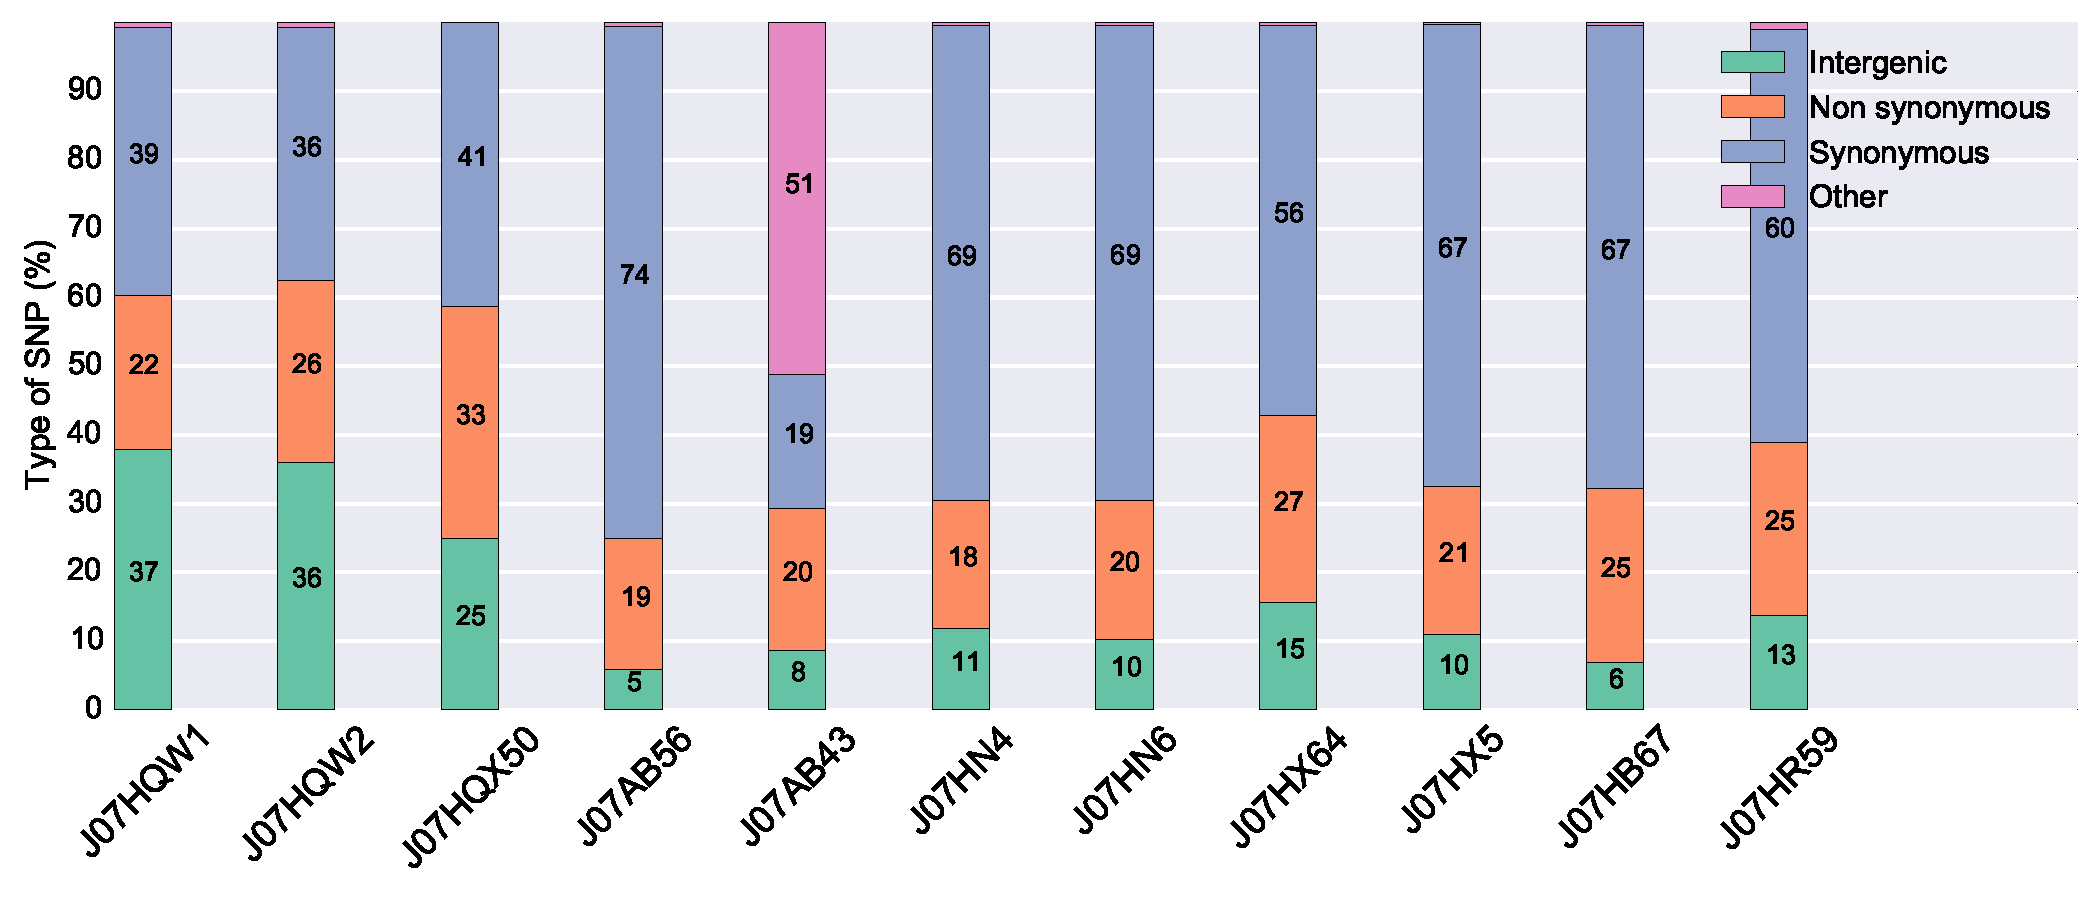
\includegraphics[width=\textwidth]{Chapter5/Figures/ReferenceSNPtypes.pdf}
%	\caption{Classification of the reference SNPs, by type.}
%	\label{ReferenceSNPsType}
%\end{figure}
%
%%FIGURE
%\begin{figure}[!htbp]
%	\centering
%	\subfloat[Total SNPs \label{COG_TotalSNPs}]{%
%		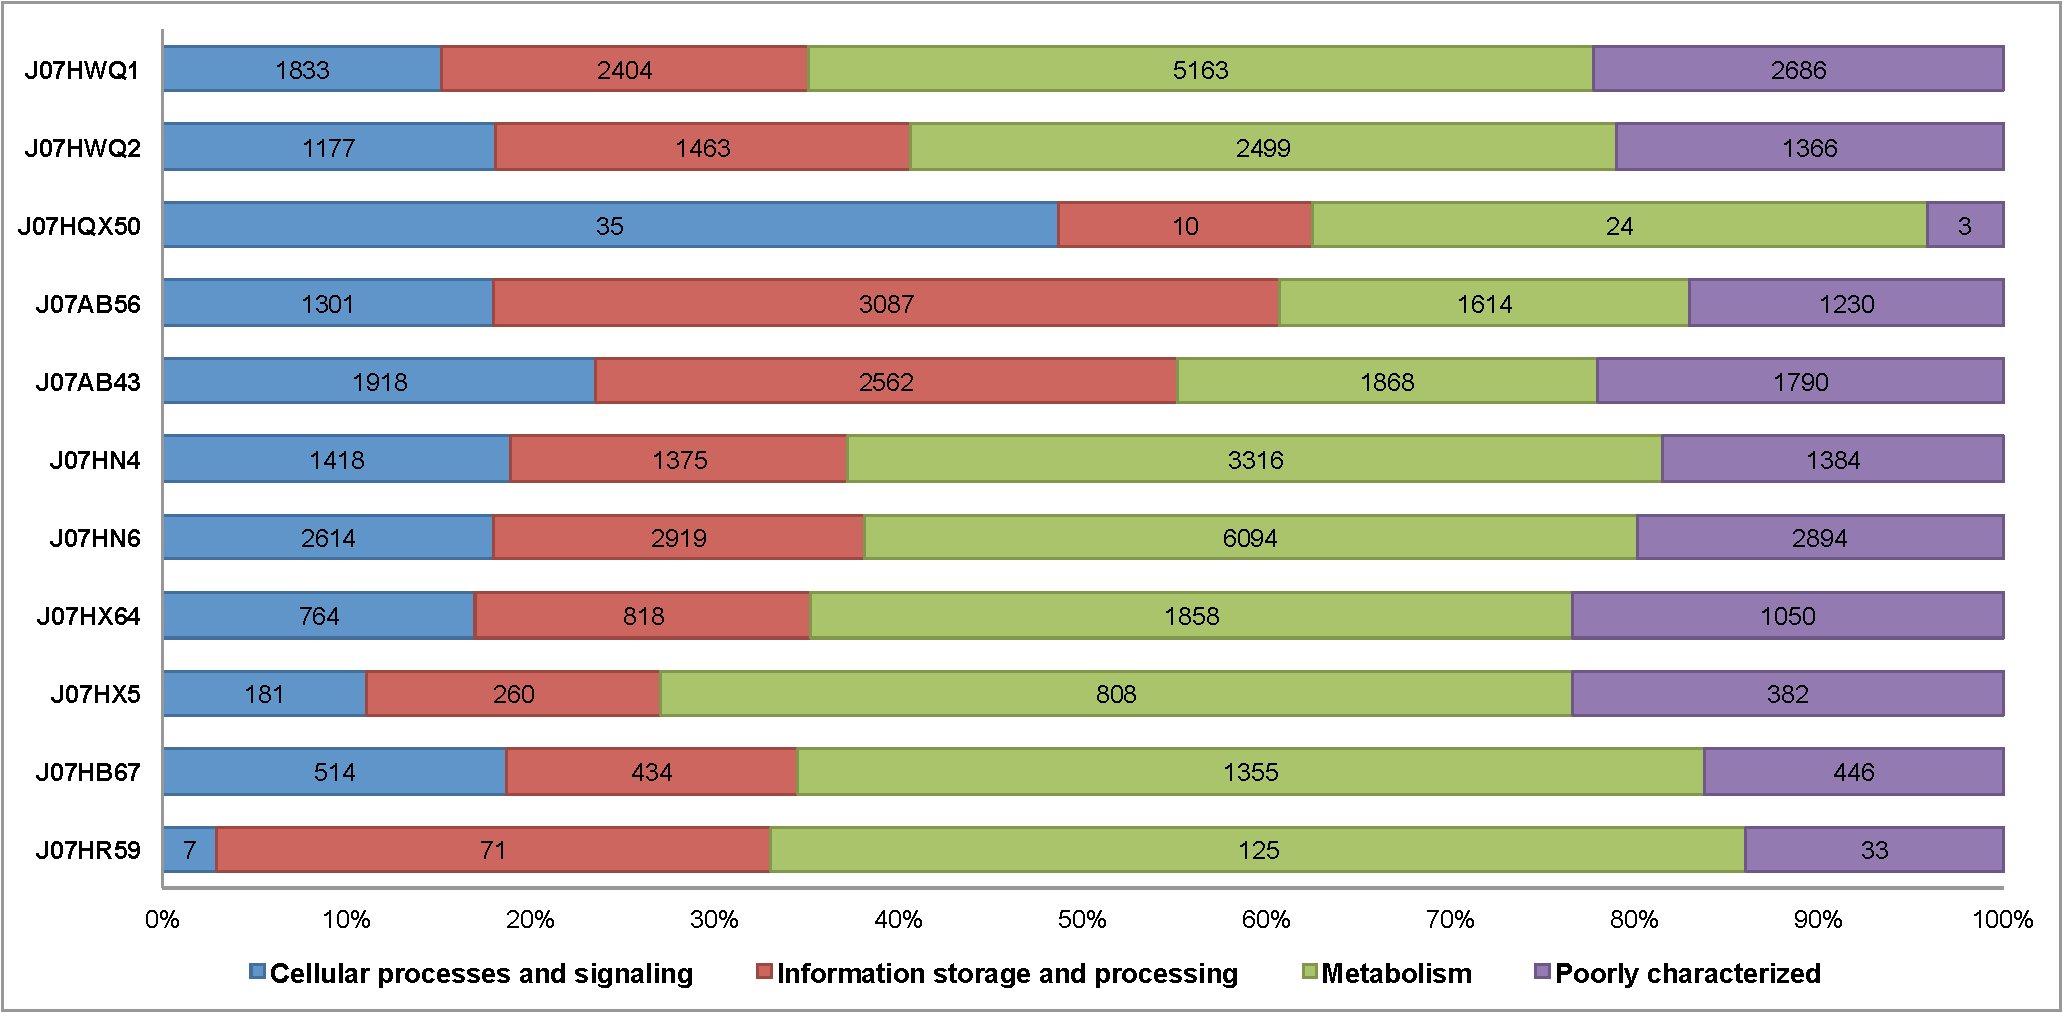
\includegraphics[width=\textwidth]{Chapter5/Figures/ReferenceSNPs_COGsTotal.pdf}
%	}
%	\hfill
%	\subfloat[Non-synonymous SNPs\label{COG_NonSynSNPs}]{%
%		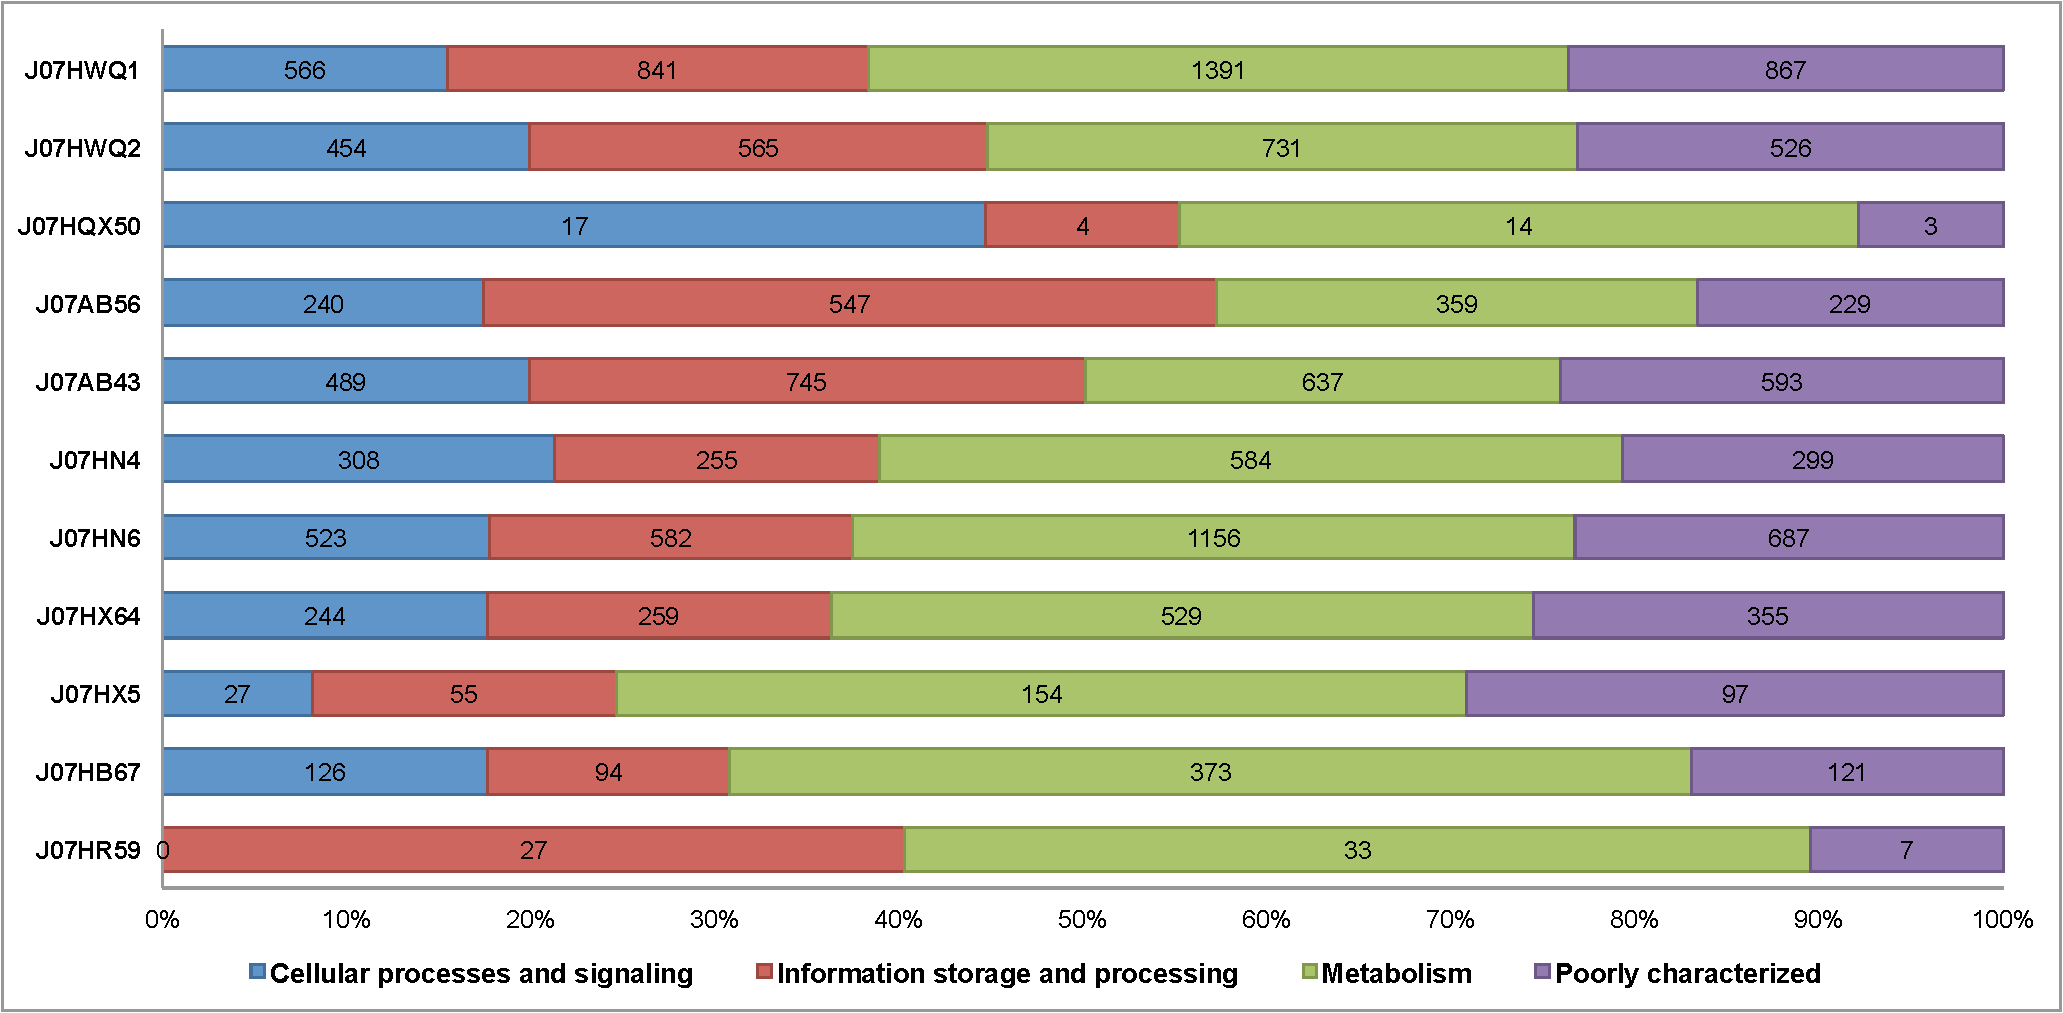
\includegraphics[width=\textwidth]{Chapter5/Figures/ReferenceSNPs_COGs_NS.pdf}
%	}		
%	\caption{Comparison between the total number and the non-synonymous SNPs found in each genome, associated to functional categories from the COG classification }
%	\label{ReferenceSNPs_COGsSummary}
%\end{figure}
%
%%FIGURE
%
%\begin{figure}[!htbp]
%	\centering
%	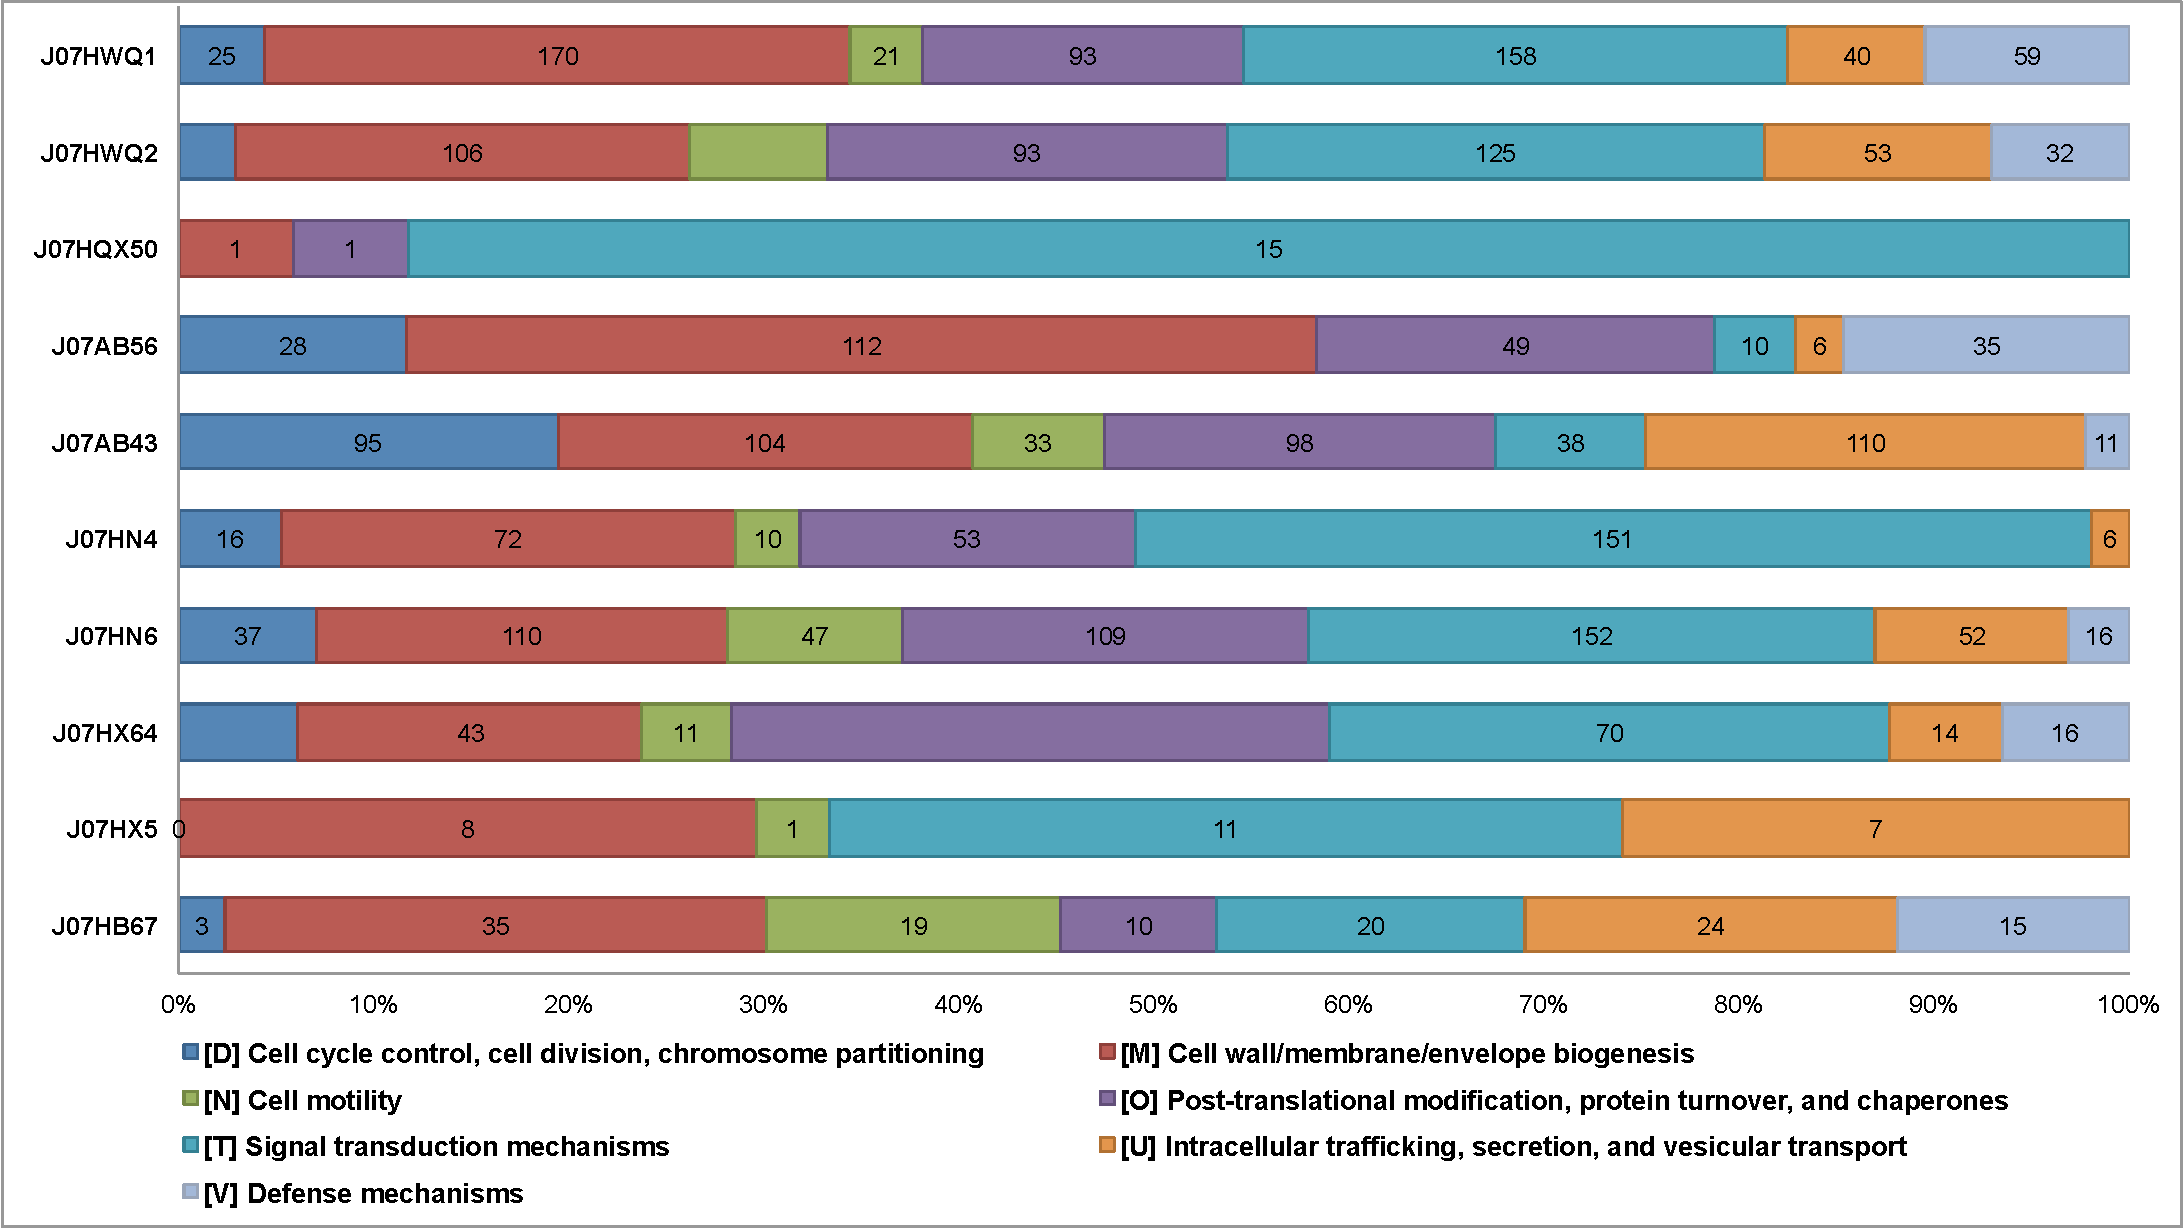
\includegraphics[width=\textwidth]{Chapter5/Figures/ReferenceSNPs_NonSyn_CellularProc.pdf}
%	\caption{Count of non-synonymous SNPs found in COGs categories from the Cellular Processes and Signaling group}
%	\label{ReferenceSNPs_NS_CellularProc}
%\end{figure}
%
%\begin{figure}[!htbp]
%	\centering
%	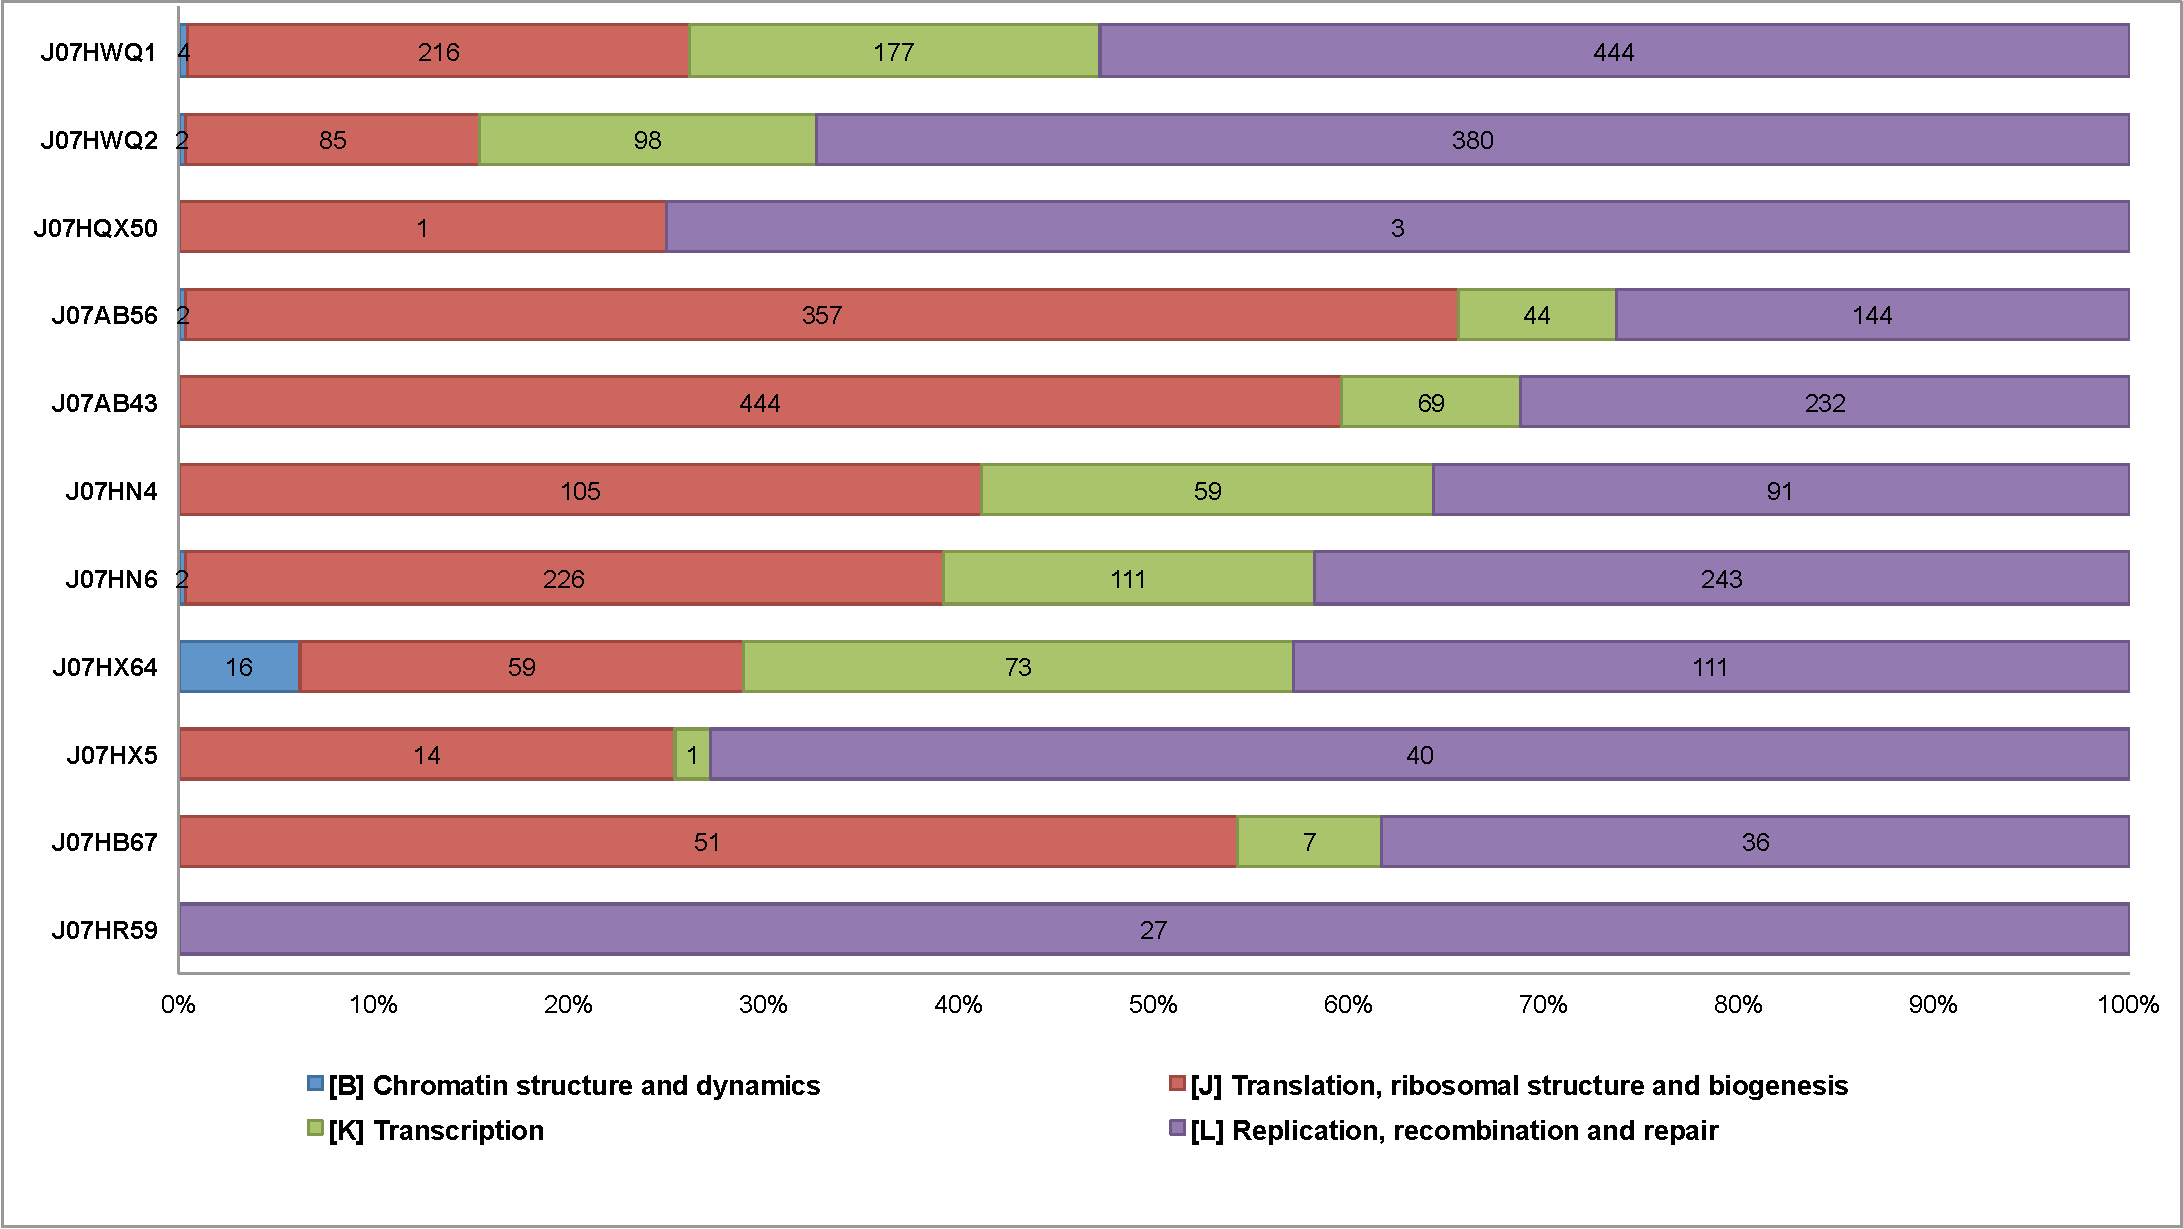
\includegraphics[width=\textwidth]{Chapter5/Figures/ReferenceSNPs_NonSyn_Information.pdf}
%	\caption{Count of non-synonymous SNPs found in COGs categories from the Information Storage and Processing group}
%	\label{ReferenceSNPs_NS_Information}
%\end{figure}
%
%\begin{figure}[!htbp]
%	\centering
%	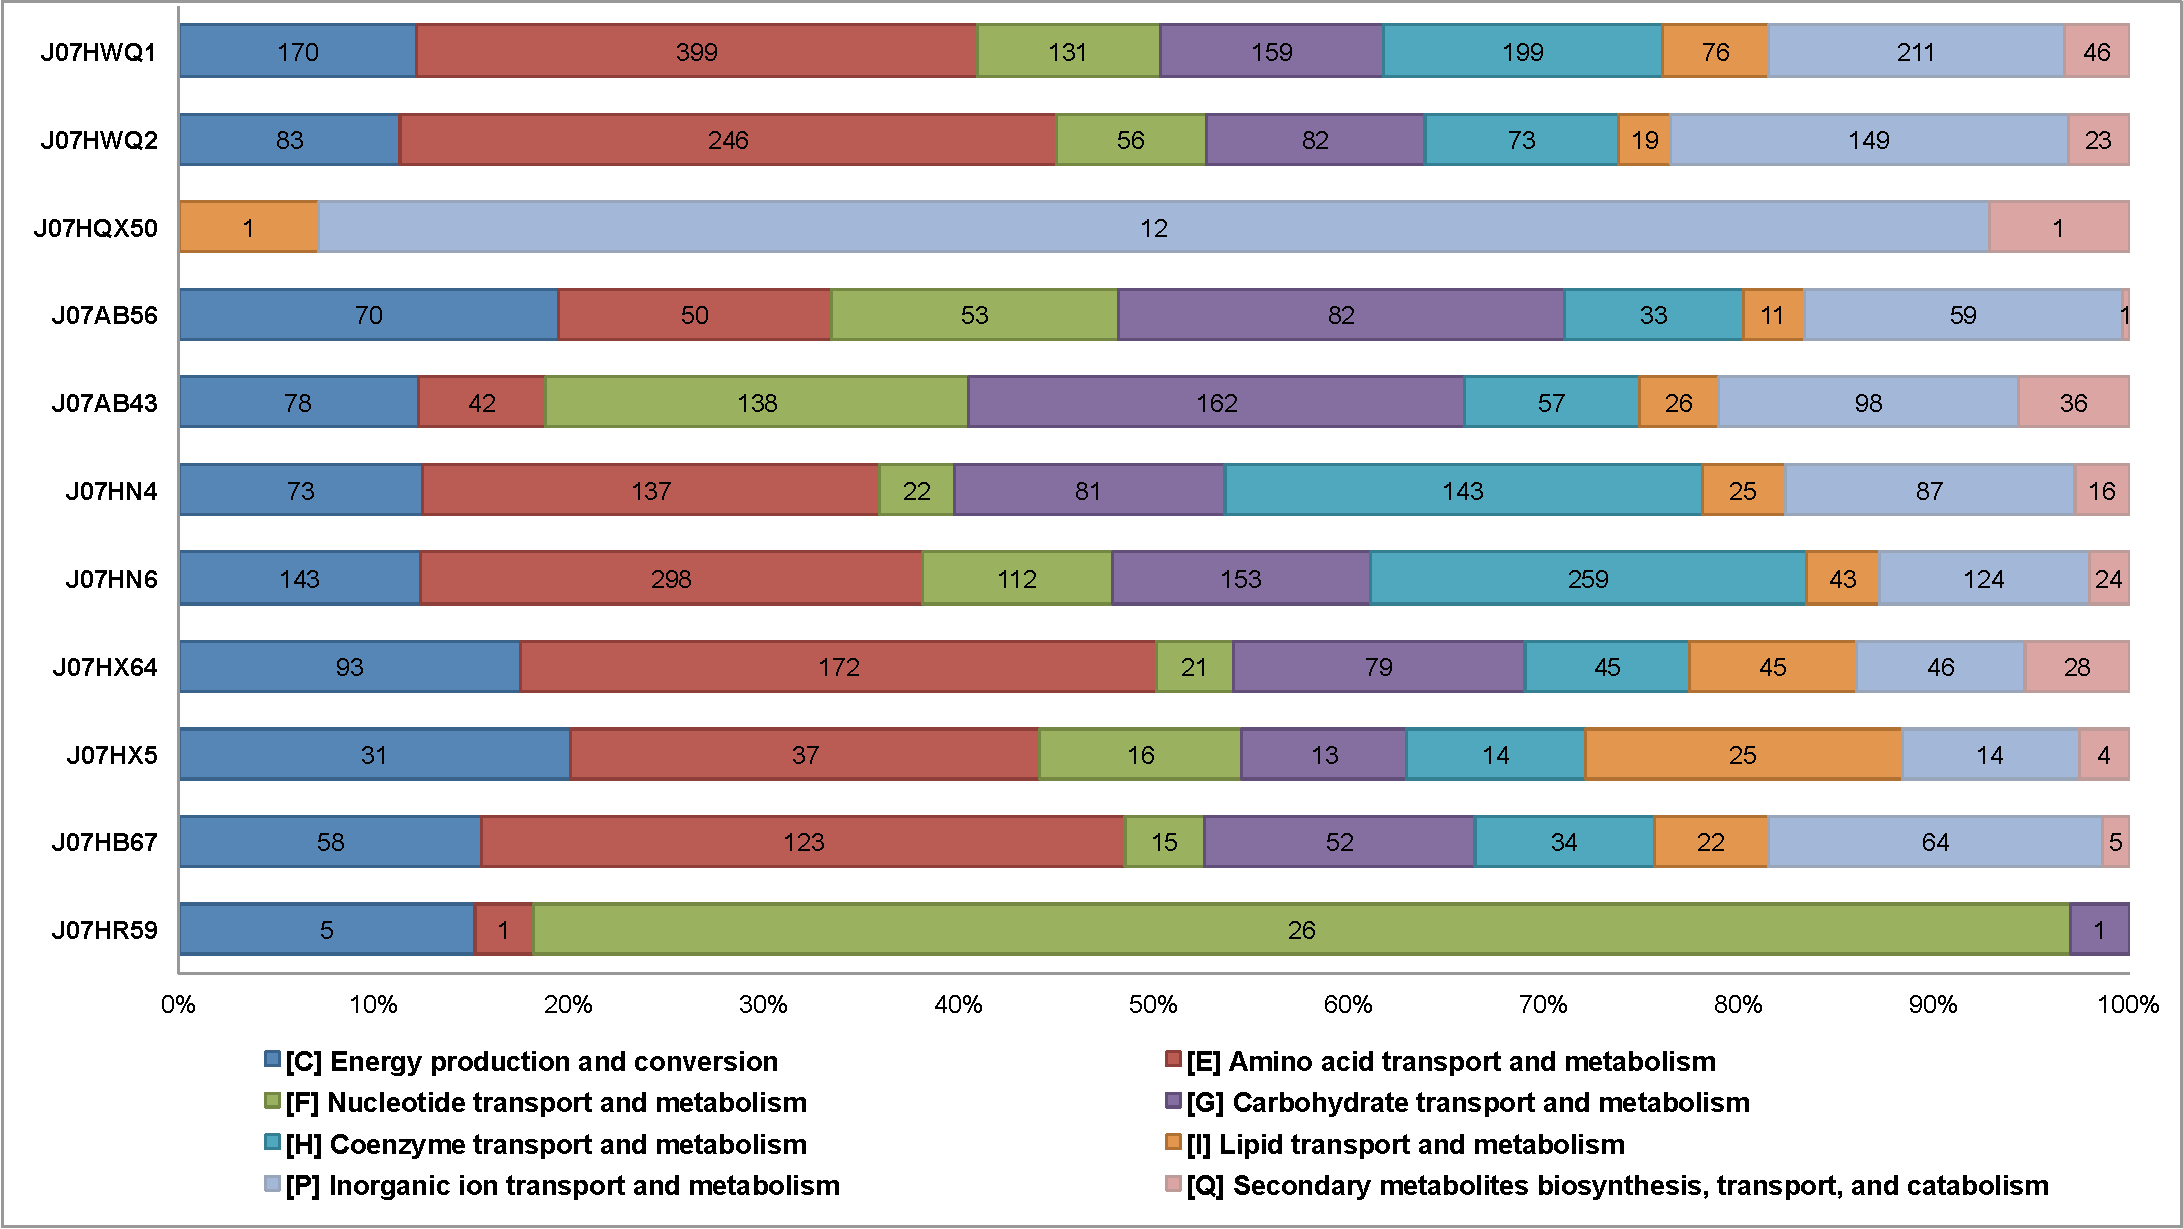
\includegraphics[width=\textwidth]{Chapter5/Figures/ReferenceSNPs_NonSyn_Metabolism.pdf}
%	\caption{Count of non-synonymous SNPs found in COGs categories from the Metabolism group}
%	\label{ReferenceSNPs_NS_Metabolism}
%\end{figure}
%
%
%

%\subsection{Selection analysis of the reference SNPs}
%- Genes found under positive selection
%- Functional differences of the genes under positive selection
%- Categories, etc

%
%
%Comparison between assembly and read mapping
%
%The comparison between the number of reads used in the assembly of the archaeal populations, versus mapping the reads back to these genomes, indicates that only a low percentage of the reads were not recovered by mapping (XX\%) (Figure X). In addition, mapping of the reads allows the recovery of reads that were not incorporated into the assemblies.
%
%Even when the number the depth of coverage is increase when the reads are mapped back to the reference genomes (Table X), the overall distribution of depths along the genome shows a similar trend (Figure X), indicating that even with that more reads are recruited (increasing the depth of coverage and posiblly the number of SNPS presents compared to an assembly-based analysis), we are not overrepreseting areas of the genome.
%
%We observed differences when looking at the coverage of individual genes, where a small percentage in each genome (XX, Table X) showed less coverage than expected. Neverhelss, this is only a small fraction of the total number of genes present (Figure X).
%
%Look at the gene with transport, secretory or motilify functions in detail. Look a the dN/dS ratiosn in a sliding window (201 bp?)
%
%For hypothetica proteins, look at SCOP classification
%


%
%\begin{figure}[htbp]
%	\centering
%	*
%	\caption{Analysis pipeline workflow}
%	\label{WorkflowAnalysisSNPs}
%\end{figure}
%
%
%\begin{figure}[htbp]
%	\centering
%	*
%	\caption{Mapped reads per genome}
%	\label{ReadMappingGenomes}
%\end{figure}
%
%\begin{figure}[htbp]
%	\centering
%	*
%	\caption{Depth of coverage for each genome}
%	\label{DepthCoverageGenomes}
%\end{figure}
%
%\begin{figure}[htbp]
%	\centering
%	*
%	\caption{SNPs in COGs}
%	\label{COGsSNPs}
%\end{figure}
%
%\begin{figure}[htbp]
%	\centering
%	*
%	\caption{Transition transversion rates}
%	\label{TTrates}
%\end{figure}
%
%\begin{figure}[htbp]
%	\centering
%	*
%	\caption{Network diagram SNPs}
%	\label{NetworkSNPs}
%\end{figure}
%
%\begin{figure}[htbp]
%	\centering
%	*
%	\caption{Map of SNPs in contigs}
%	\label{SNPsContigMap}
%\end{figure}
%
%\begin{figure}[htbp]
%	\centering
%	*
%	\caption{SNP rarefaction curve per population}
%	\label{SNPsRarefaction}
%\end{figure}
%
%\begin{figure}[htbp]
%	\centering
%	*
%	\caption{Calculation of pN/pS ratios}
%	\label{pNpS_diagram}
%\end{figure}
%
%\begin{figure}[htbp]
%	\centering
%	*
%	\caption{Histogram of dN/dS ratios}
%	\label{pNpS_hist}
%\end{figure}


%Figure SNPs in genes
%\begin{figure}[h]
%\centering
%\subfloat[January (both dates combined)]{
%    \label{Jan_SNP_boxplot}
%    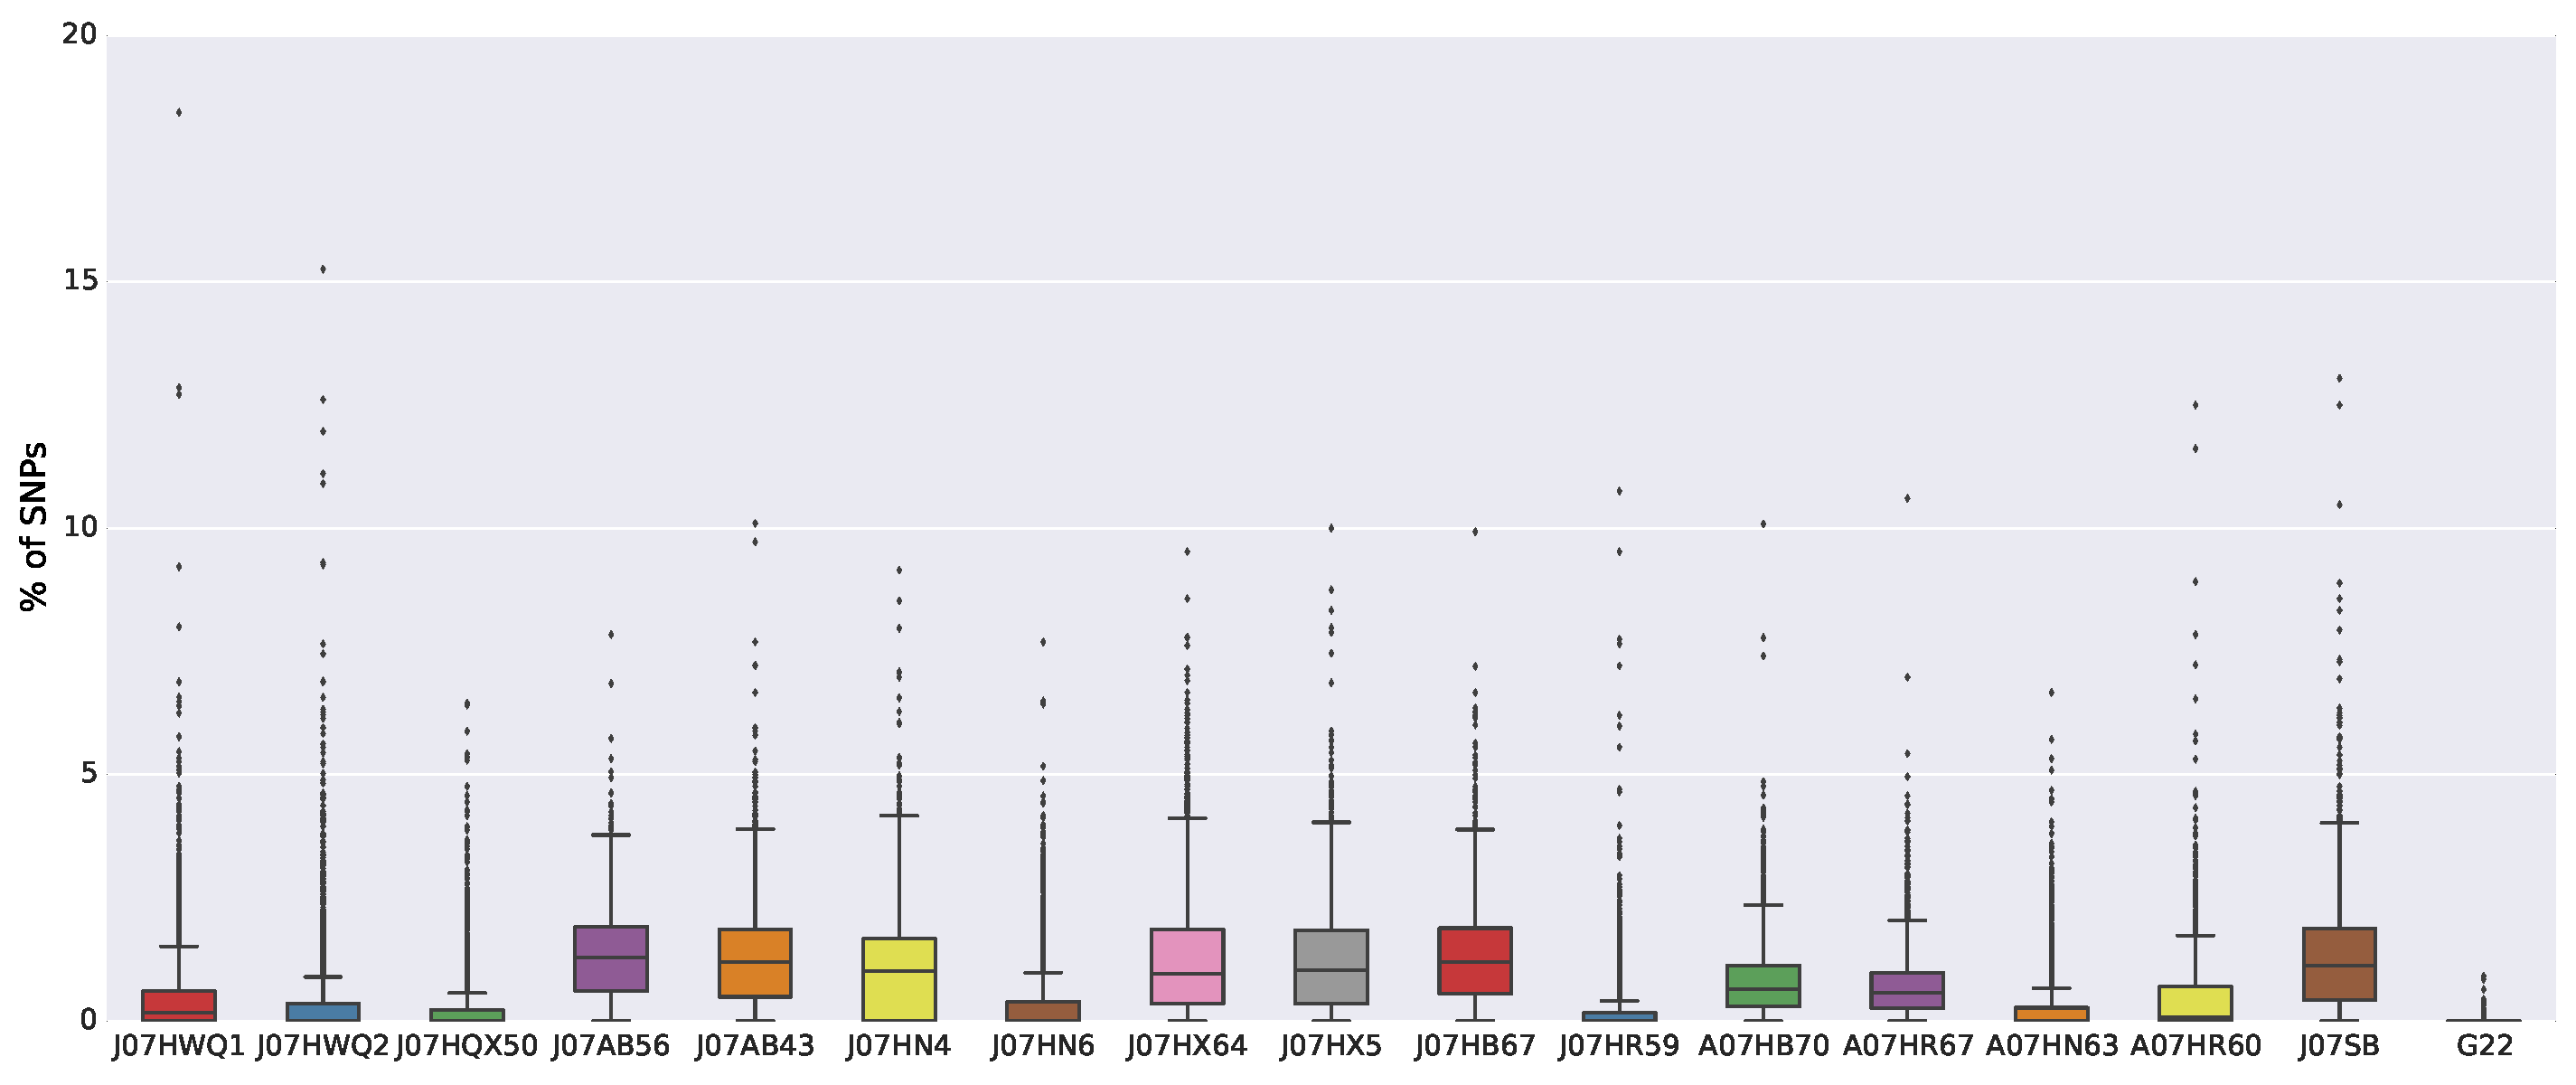
\includegraphics[width=\textwidth]{Chapter5/Figures/Jan_SNP_freq_boxplot.pdf}
%    }
%    \hfill
%\subfloat[August (both dates combined)]{
%    \label{Aug_SNP_boxplot}
%    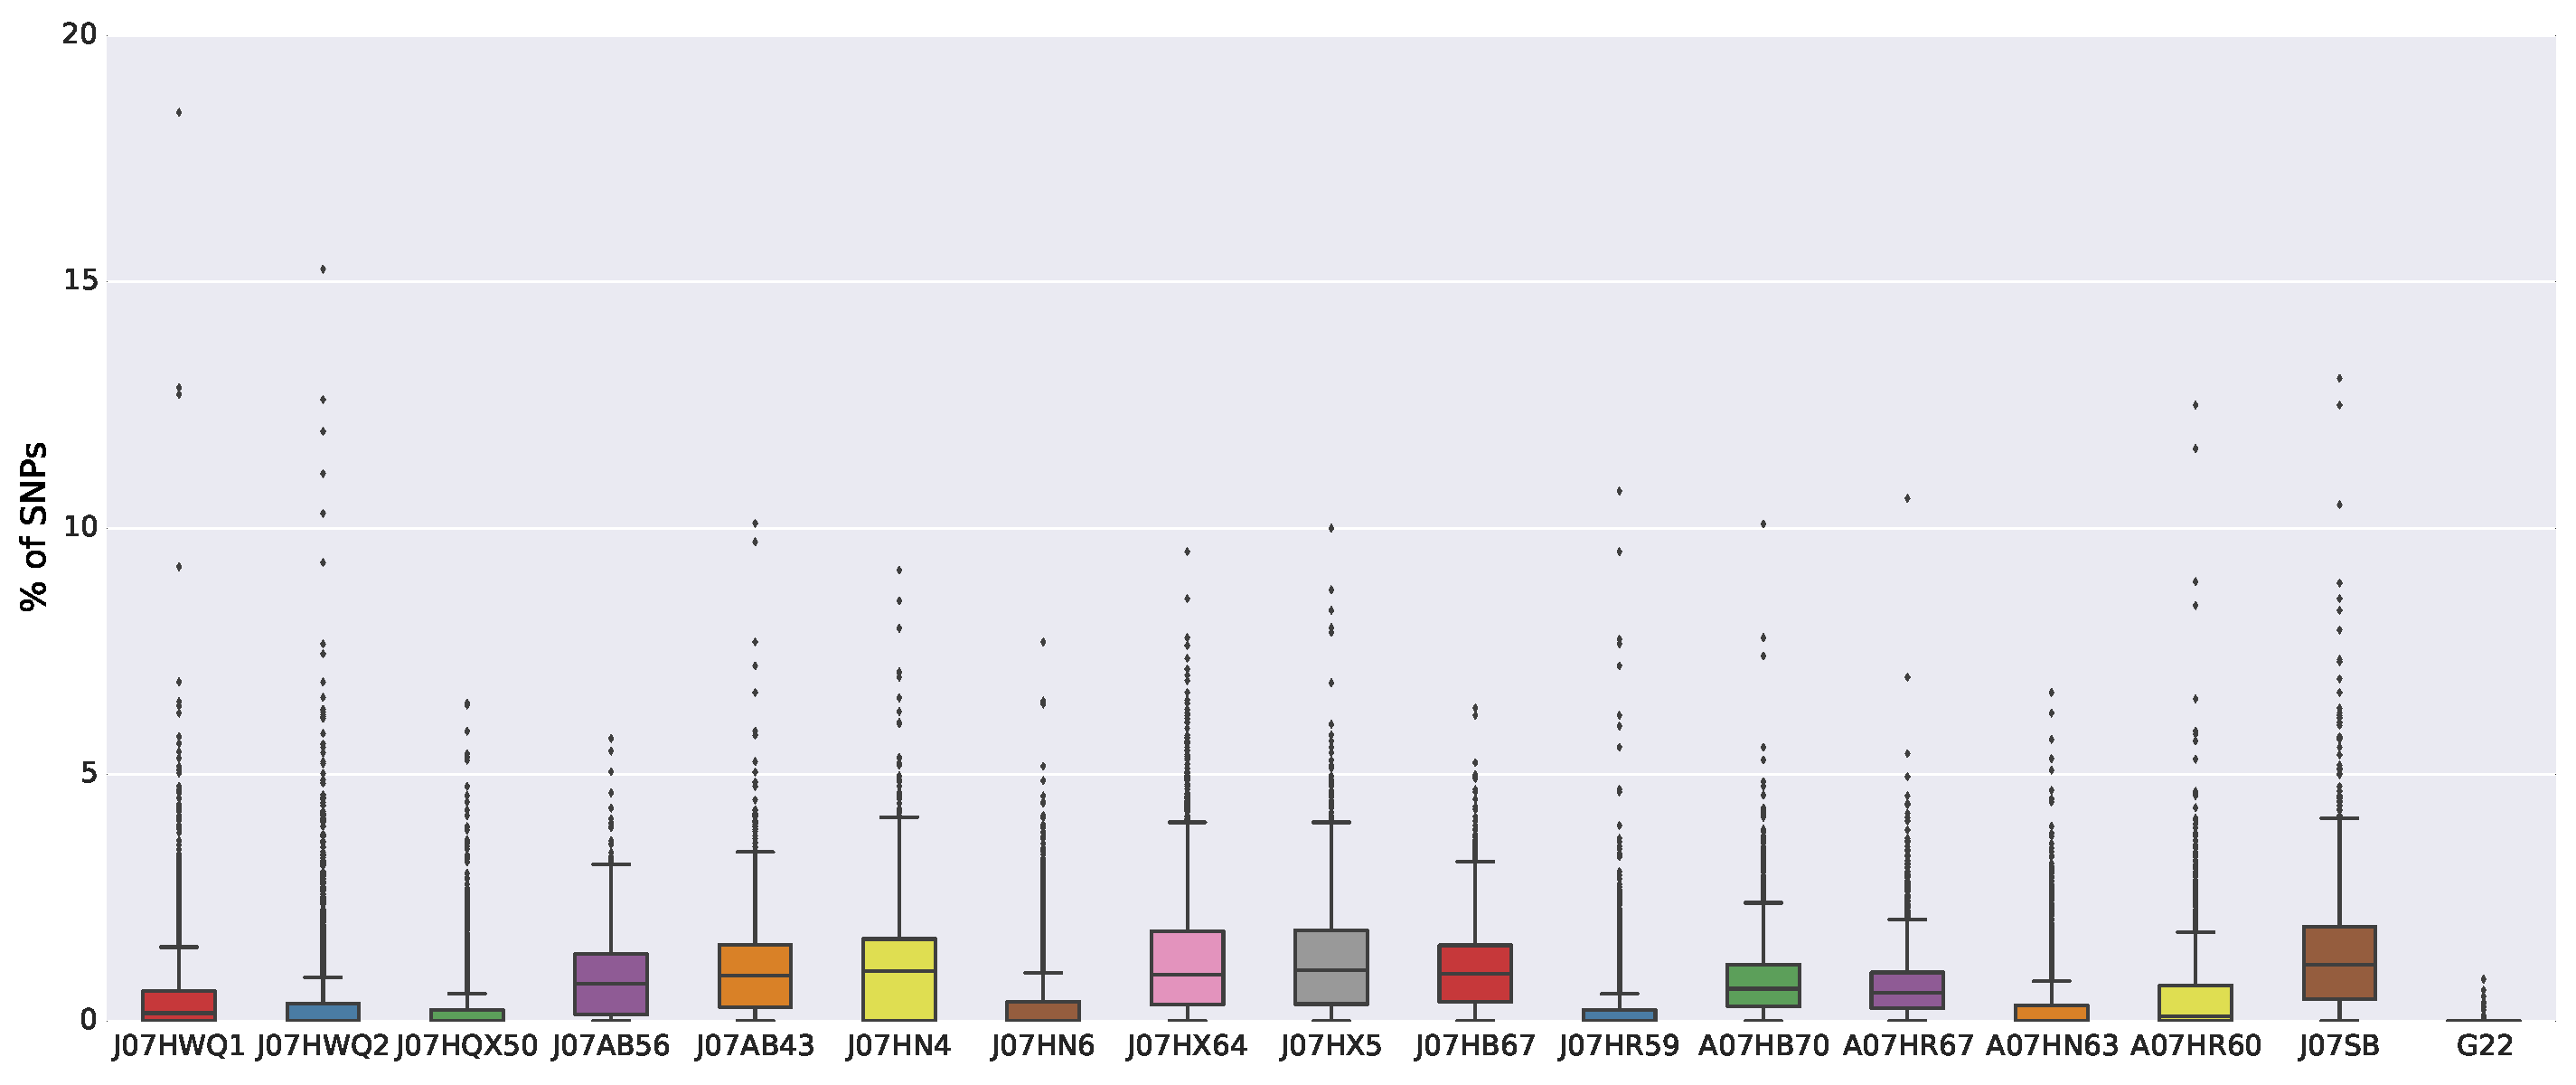
\includegraphics[width=\textwidth]{Chapter5/Figures/Aug_SNP_freq_boxplot.pdf}
%    }
%    \caption{Distribution of genes based on the percentage of SNPs present in them, in the January and August combined libraries.}
%    \label{SNPs_Boxplot}
%\end{figure}


%\bibliographystyle{abbrv}
%\bibliography{CompleteLibrary}

%Chapter 6
%\chapter{Comparative genomics and selective pressure analysis; analysis of the \textit{Haloquadratum walsbyi} genome}

\section{Abstract}

\section{Introduction}

With the development of neovel sequencing technologies, the price to sequence a single microbial genome has decreased considerable over the last years \cite{Mardis:2013gn}, increasing the number of microbial genomes in databases, helping investigation of comparative genomics, etc, etc. (REFs). 

More genomes for related strains, and related species.

Whole genome analysis allows to increase phylogenetic resolution among multiple groups, and also to start asking questions about the particular genomic features that affect the adaptation of each organism to the environment.

Now is possible to move from comparing a single genome to several (REFs)

Multiple databases exist where genomes have been compared and the data is already available in pre-calculated databases (REFs), but in some cases it is difficult to add or analyze recent genomes. A recent software ITEP, allows these comparasions. PSP allows also this, but is a web server

Selection analysis are important, not only gene content (absecnce presence)

In this chapter, I describe a pipeline developed for the comparative analysis of microbial genomes, with an emphasis on pan-genome anlaysis and selection analysis. All of the code is freely available in Github (link), and is currently being updated to be applied to large scale comparisons (~100 genomes). 

\section{Overview of the analysis workflow}

The analysis strategy consists on several Python scripts that carry out the different steps of data analysis (Figure \ref{CompGenomePipeline}). All of the scripts are available in a public repository on Github (\url{http://github.com/juanu/CompMicroGenom}). The analysis steps can be summarized as:

\begin{itemize}
\item Data preprocessing
\item Ortholog search
\item Analysis of ortholog data
\item Selection analysis
\item Result summary
\end{itemize}

In the following sections, each of these steps will be explained in more detail.

\begin{figure}[htbp]
	\centering
	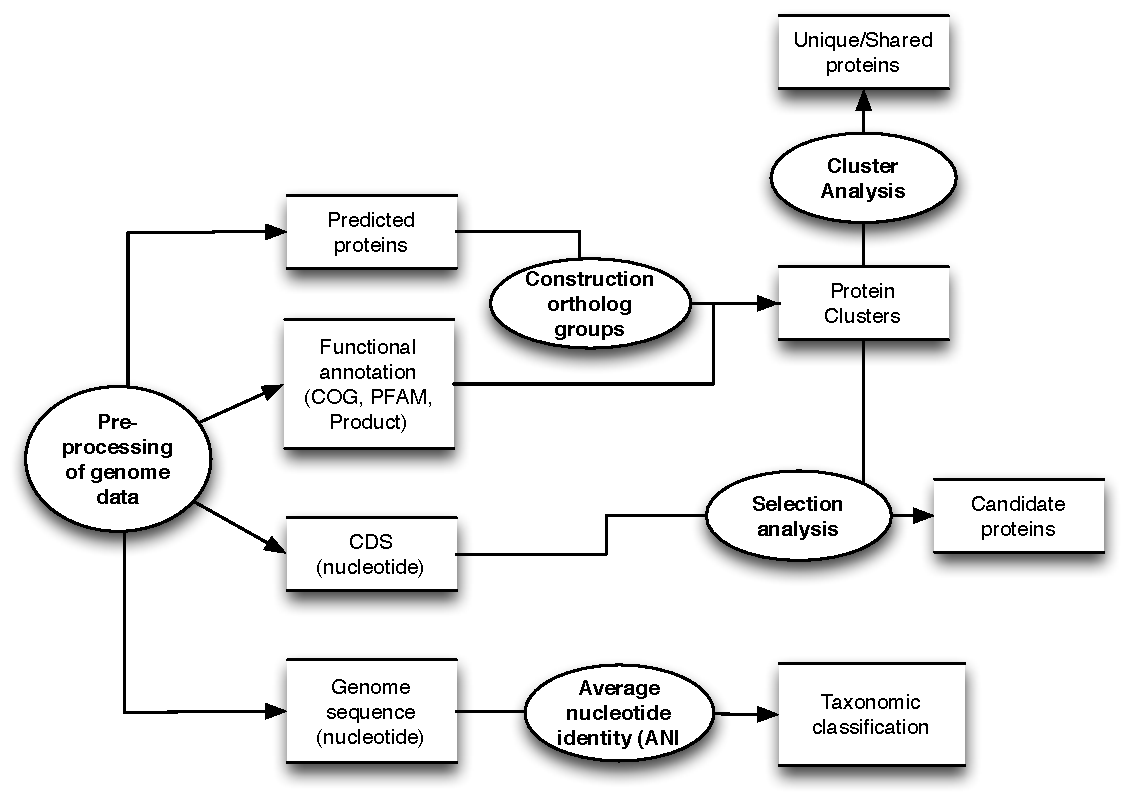
\includegraphics[width=\textwidth]{Chapter6/Figures/WorkflowOverview.pdf}
	\caption[Overview of the pipeline developed for the comparative analysis of microbial genomes]{Overview of the pipeline developed for the comparative analysis of microbial genomes.}
	\label{CompGenomePipeline}
\end{figure}

\subsection{Data preprocessing}

Several public resources are available for genome annotation and as repositories. Among some of the most used ones are the Integrated Microbial Genomes database\cite{Markowitz:2011ck}, NCBI and RAST \cite{Aziz:2008ku}. Although some of these repositories overlap in their content (in particular IMG and NCBI), the increase in the rates of submission of newer genomes, makes IMG slightly outdated in comparison to other resources. On the other hand, some of the genomes that are present on IMG are not available on NCBI and/or RAST. To be able to exploit all these available information, a pre-processing step is incorportated in the analysis to parse genomes obtained from these different sources, and put them into a common format that can be easily used through all the workflow (Figure \ref{Preprocessing}). Using this strategy, also allows to incorporate genomes from newer sources, by just adding a new parsing script. For example, it could be relatively easy to incorporate an in-house sequenced genome into this workflow, by using a genome annotation pipeline like Prokka \cite{Seemann:2014ks}, and connecting into this workflow.

\begin{figure}[htbp]
	\centering
	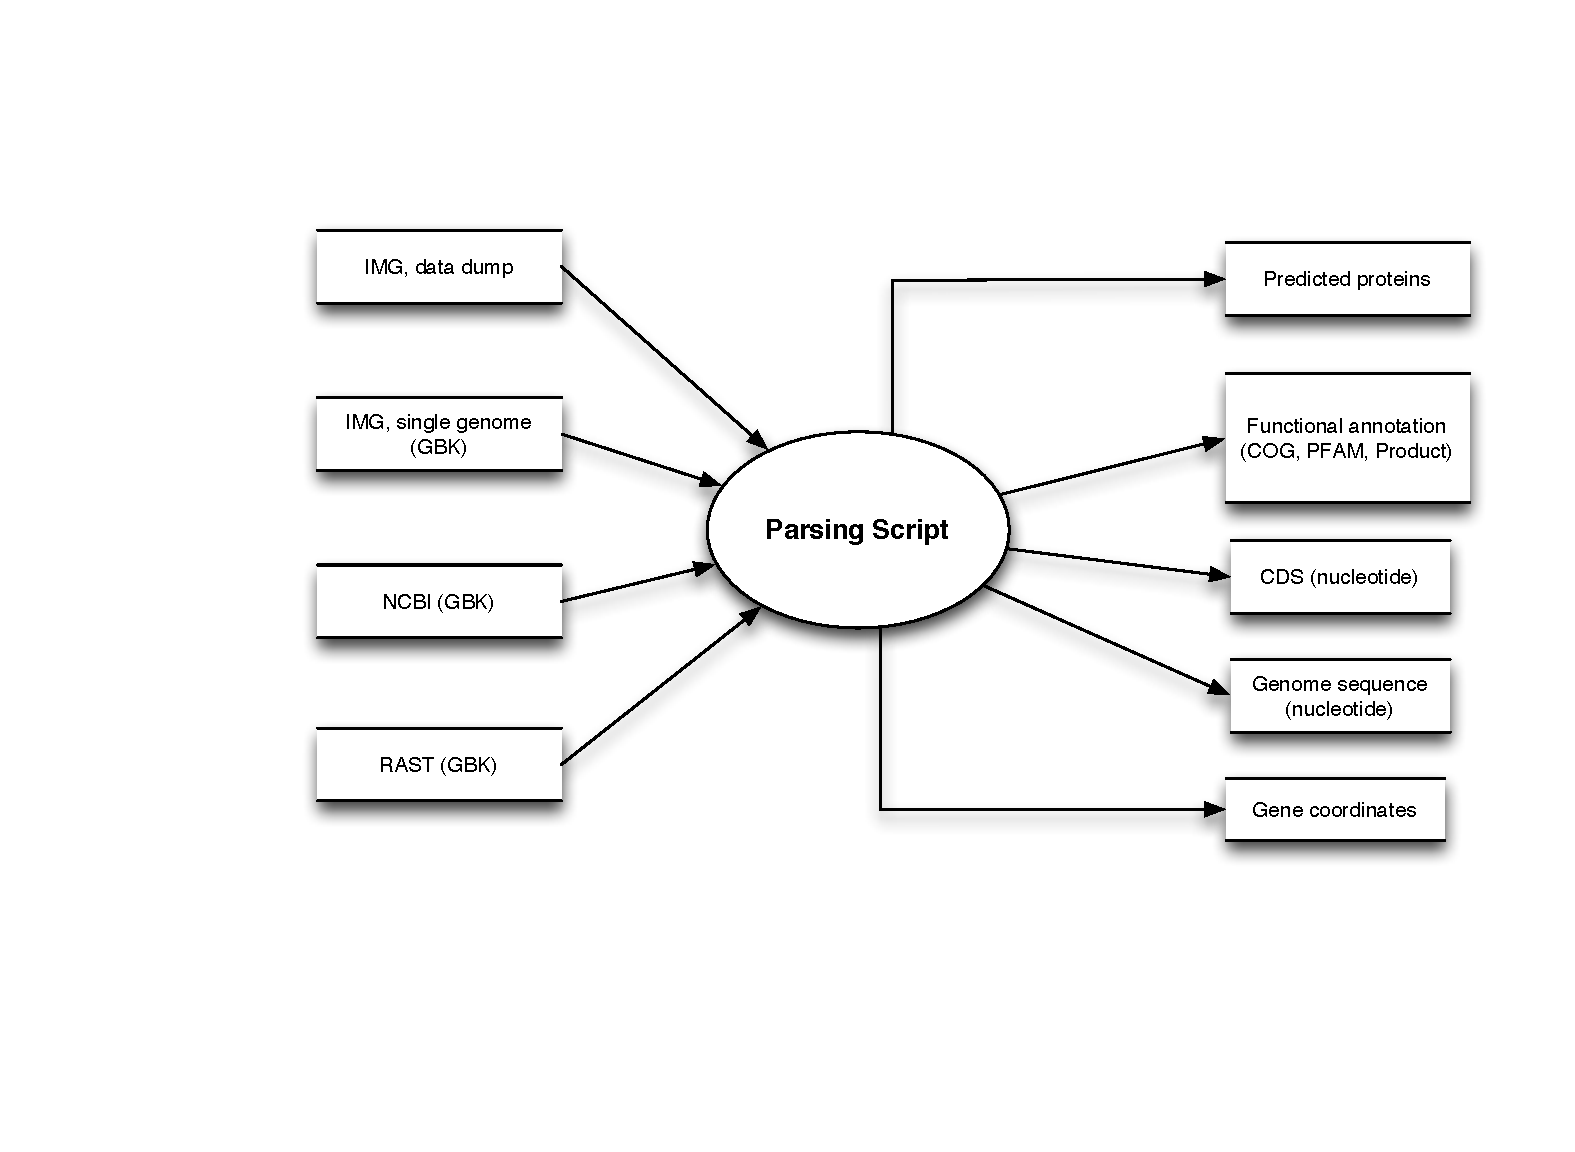
\includegraphics[width=\textwidth]{Chapter6/Figures/PreprocessingOverview.pdf}
	\caption{Preprocessing step}
	\label{Preprocessing}
\end{figure}

\subsection{Construction of orthologous groups}

The basis of this comparative genomic approach is the construction of orthologous groups of genes, a collection of all the descendants of an ancestral gene that diverged after a given speciation event  \cite{Kristensen:2011gw}. These groups provide us with a picture of the evolutionary history of the gene family (and its host organisms), and can be used for further studies on the basis for molecular adaptation of its host organisms.
Several approaches exists for the construction of ortholog groups \cite{Kristensen:2011gw}, which can be broadly classified in two categories: tree-based and heuristic based approaches. Tree based methods are computationally expensive and require a known phylogenetic relationship for the studied organisms, something that sometimes is difficult to generate in light of the presence of horizontal gene transfer events in microbial genomes \cite{Koonin:2001vz}. On the other hand, heuristic based approaches are easy to automatize and several implementations of these methods are already available \cite{Kristensen:2011gw}. Among the main drawbacks, the generated group of sequences may not reflect the true evolutionary history of the gene, specially in large and complicated protein families \cite{Chen:2007kk}.
In consideration of this evidence, we choose an heuristic-based approach to generate orthologous groups, because it can be easily scalable to hundreds of genome, and its easiness to incorporate into an automatic pipeline. OrthoMCL \cite{Li:2003en}, performs a bidirectional best hit search in the aminoacid space, using a "all-vs-all" blastp (although, other search methods could be implemented), followed by a subsequent clustering of the results using a Markov Clustering procedure \cite{Enright:2002uq}.

Within the current workflow, the construction of ortholog groups is based on the OrthoMCL protocol \cite{Li:2003en}, consisting of the following steps: 
\begin{itemize}
\item Protein blast of "all-vs-all" the proteins
	\begin{itemize}
	\item Concatenate all the protein sequences for the genomes of interest
	\item Create a Blast database
	\item Protein blast using these parameters: \textit{-F 'm S' -v 1000000 -b 1000000 -m 8}
	\end{itemize}
\item OrthoMCL analysis
	\begin{itemize}
	\item Create a MySQL database to store the OrthoMCL results
	\item Run OrthoMCL to generate a list containing pairs of sequences and their similarity score
	\item Use MCL to create clusters based on the previous results. Different inflation values can be tested, where smaller values give larger clusters.
	\end{itemize}
\end{itemize}

\subsection{Analysis of ortholog groups}

The clusters of sequences obtained from the previous step are processed using a set of Python scripts to summarize the results. Some of the information obtained here includes:

\begin{itemize}
\item List and count of unique sequences in each analyzed genomes
\item A list and count of single copy clusters; sequences that are present in single copy in all the analyzed genomes. 
\item A list and count of shared multiple copy clusters; sequences present in all the analyzed genomes, but that in some of them are present in more than one copy.
\end{itemize} 

Levering on these cluster results, several analysis can be performed using this information:

\subsubsection{Functional annotation}

The resulting protein clusters can be annotated, based on the information obtained from the annotation files. Currently the annotation incorporates information such as Cluster of Orthologous Groups (COGs), KEGG (REF) and PFAM domains (REF). The current approach for the annotation is to use a majority rule for the cluster, where each cluster is annotated with the function that half plus one of the proteins in the cluster have. This also serves as a validation step, because in classifications such as COGs, is expected that all of the members from the cluster should have the same COG number. Conflicts are recorded for validation as well.

\subsubsection{Alignment and tree construction}

As part of the pipeline, it is possible to generate alignments and trees for all (or a subset) of the clusters generated. The approach used is to generate an alignment of each cluster using MAFFT on the amino acid sequences, followed by a construction of a phylogenetic tree using FastTree. DNA alignments are generated by replacing each amino acid in the aligned sequences, with its corresponding codon from the DNA sequences, allowing for better DNA alignments. All of the resulting sequences (aligned and unaligned) are saved for future reference.

\subsubsection{Phylogenomic analysis}

One of the most important goals of the workflow is to generate information useful for phylogenomic analysis. Phylogenetic classification based on 16S rRNA sequences, lathough highly used, are limited by the sequence space of the 16S rRNA gene. Even species with highly similar 16S rRNA sequences, show differences both in their gene content and the functional capabilities. The use of marker genes, multi-locus sequence typing (MLST) and whole genome analysis, allow to increase the information and therefore the resolution of phylogenetic classifications. 

Within the scope of the workflow, the idea is to be able to identify clusters that are present in single copy and are shared across all the genomes in the analysis. This approach is similar to what has been done for taxonomic and metagenoomic clasification of novel organisms (REF), but in this particular case allows to establish the relationships among the organisms under study. The approach used is very similar to previously proposed analysis (REF, acinetobacter), summarized on Figure \ref{PhylogenomicOverview}. All the single copy clusters are identified and the alignments of each one is generated. Each aligned cluster is tested for recombination using the Phipack software, with three different analysis PHI, MaxChi and Neighbour similarty scores (REF), with 1000 permutations, window size of 50 nt and a p-value < 0.05. The goal of this step is to select recombination free clusters that can be used for phylogenetic analysis, with the bonus by-product of identifying clusters that have evidence of recombination and could be interesting candidates for further analysis (REFs). The alignments of this recombination-free clusters are then trimmed using Gblocks with default parameters. The trimmed clusters are then concatenated to generate a newer alignment that can be used for phylogenetic analysis.

Complementary to this, another script allows to perform genomic comparisons among the studied organisms using the average nucleotide identity (ANI) between them. The approach used is the the method proposed by Goris et al (REF). For each query, two genomes are compared, where the query genome is divided into 500 bp. fragments and then compared using blastn against the target genome. For each fragment, the best hit (highest bit score) is selected if it had at least 70\% identity and covers over 70\% of the query fragment length. The pairwise comparisons are then collected into a matrix that can be used to evaluate pair of genomes and also for dendrogram construction.

\subsubsection{Population and selection}

-Why the search of this is important 
One of the most important feautres of the anlaysis is the search for clusters with evidence of selective pressure. For this PAML was used
- Statistic models
- Comparisons branch -sites

-FDR correction for multiple testing


\section{Comparative analysis of \textit{Haloquadratum}}

\subsection{\textit{Haloquadratum} core and accessory genome}

\subsection{Evidence of habitat-selection in \textit{H. walsbyi}}

\section{Conclusions and Future Directions}

General goals of the pipeline.
Goals to complete, including integrations with other tools, documentation. Use of a database for the analysis. Integration of faster tools for slection analysis.
Comparison: concatenation of proteins versus consensus of gene trees.


\begin{figure}[htbp]
	\centering
	*
	\caption{HQPanGenome}
	\label{HQPanGenome}
\end{figure}

\begin{figure}[htbp]
	\centering
	*
	\caption{Circular plot}
	\label{HQCircularPlot}
\end{figure}

%Tables
\begin{table}[htdp]
\caption{Genes under selection in HQ strains}
\begin{center}
\begin{tabular}{|c|c|}

\end{tabular}
\end{center}
\label{SelectionHQ}
\end{table}%


\section{Acknowledgments}

%\bibliographystyle{abbrv}
%\bibliography{CompleteLibrary}

\bibliographystyle{abbrv}
\bibliography{CompleteLibrary}



\appendix

\chapter{Draft Genome Sequence of “\textit{Candidatus} Halobonum tyrrellensis” Strain G22, Isolated from the Hypersaline Waters of Lake Tyrrell, Australia}\label{G22Genome}
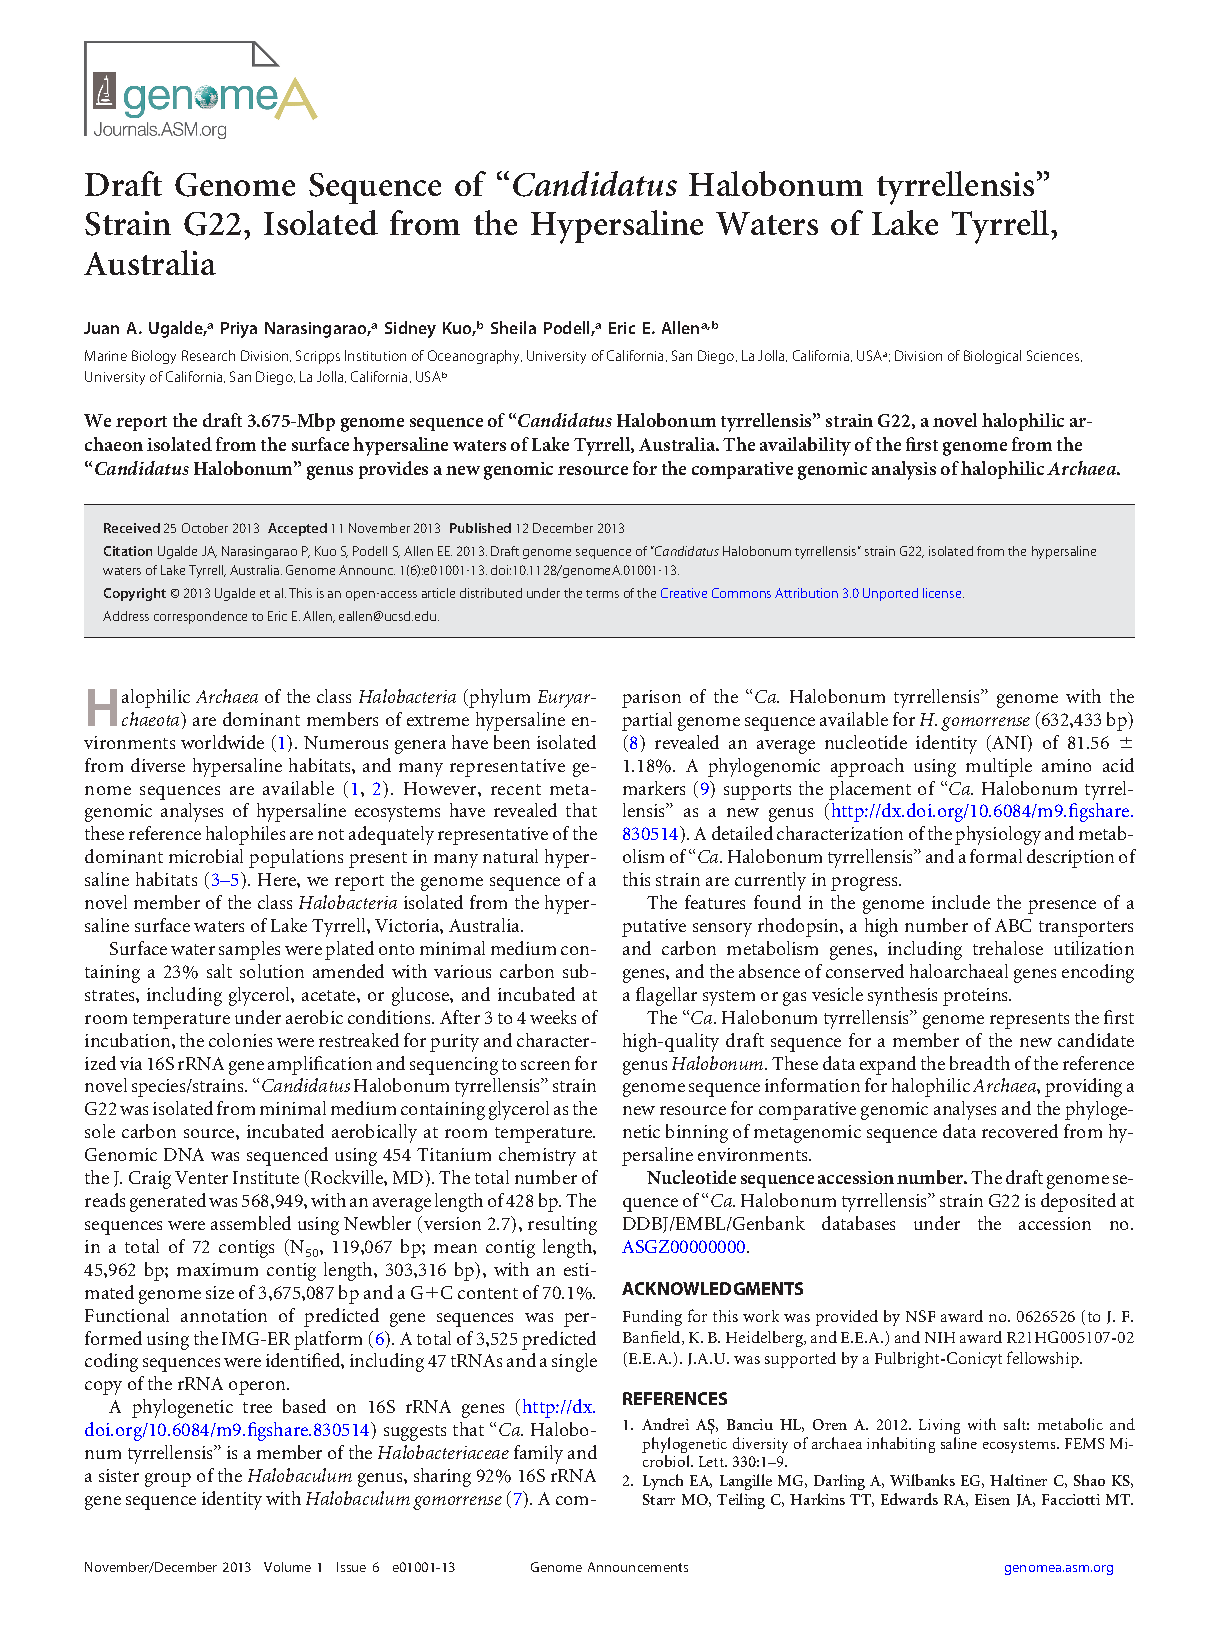
\includepdf[pages={-},fitpaper=true,scale=0.75,pagecommand={}]{Appendix/UgaldeGA_2013.pdf}
Appendix \ref{G22Genome} is a full reprint of the publication XXXX, with permissions from all coauthors.

\chapter{Genome coverage plots}
%%%%%%%%%%%%%
%Coverage plots
%Identity figures, uncomment
\begin{figure}[!hbtp]
  \centering
  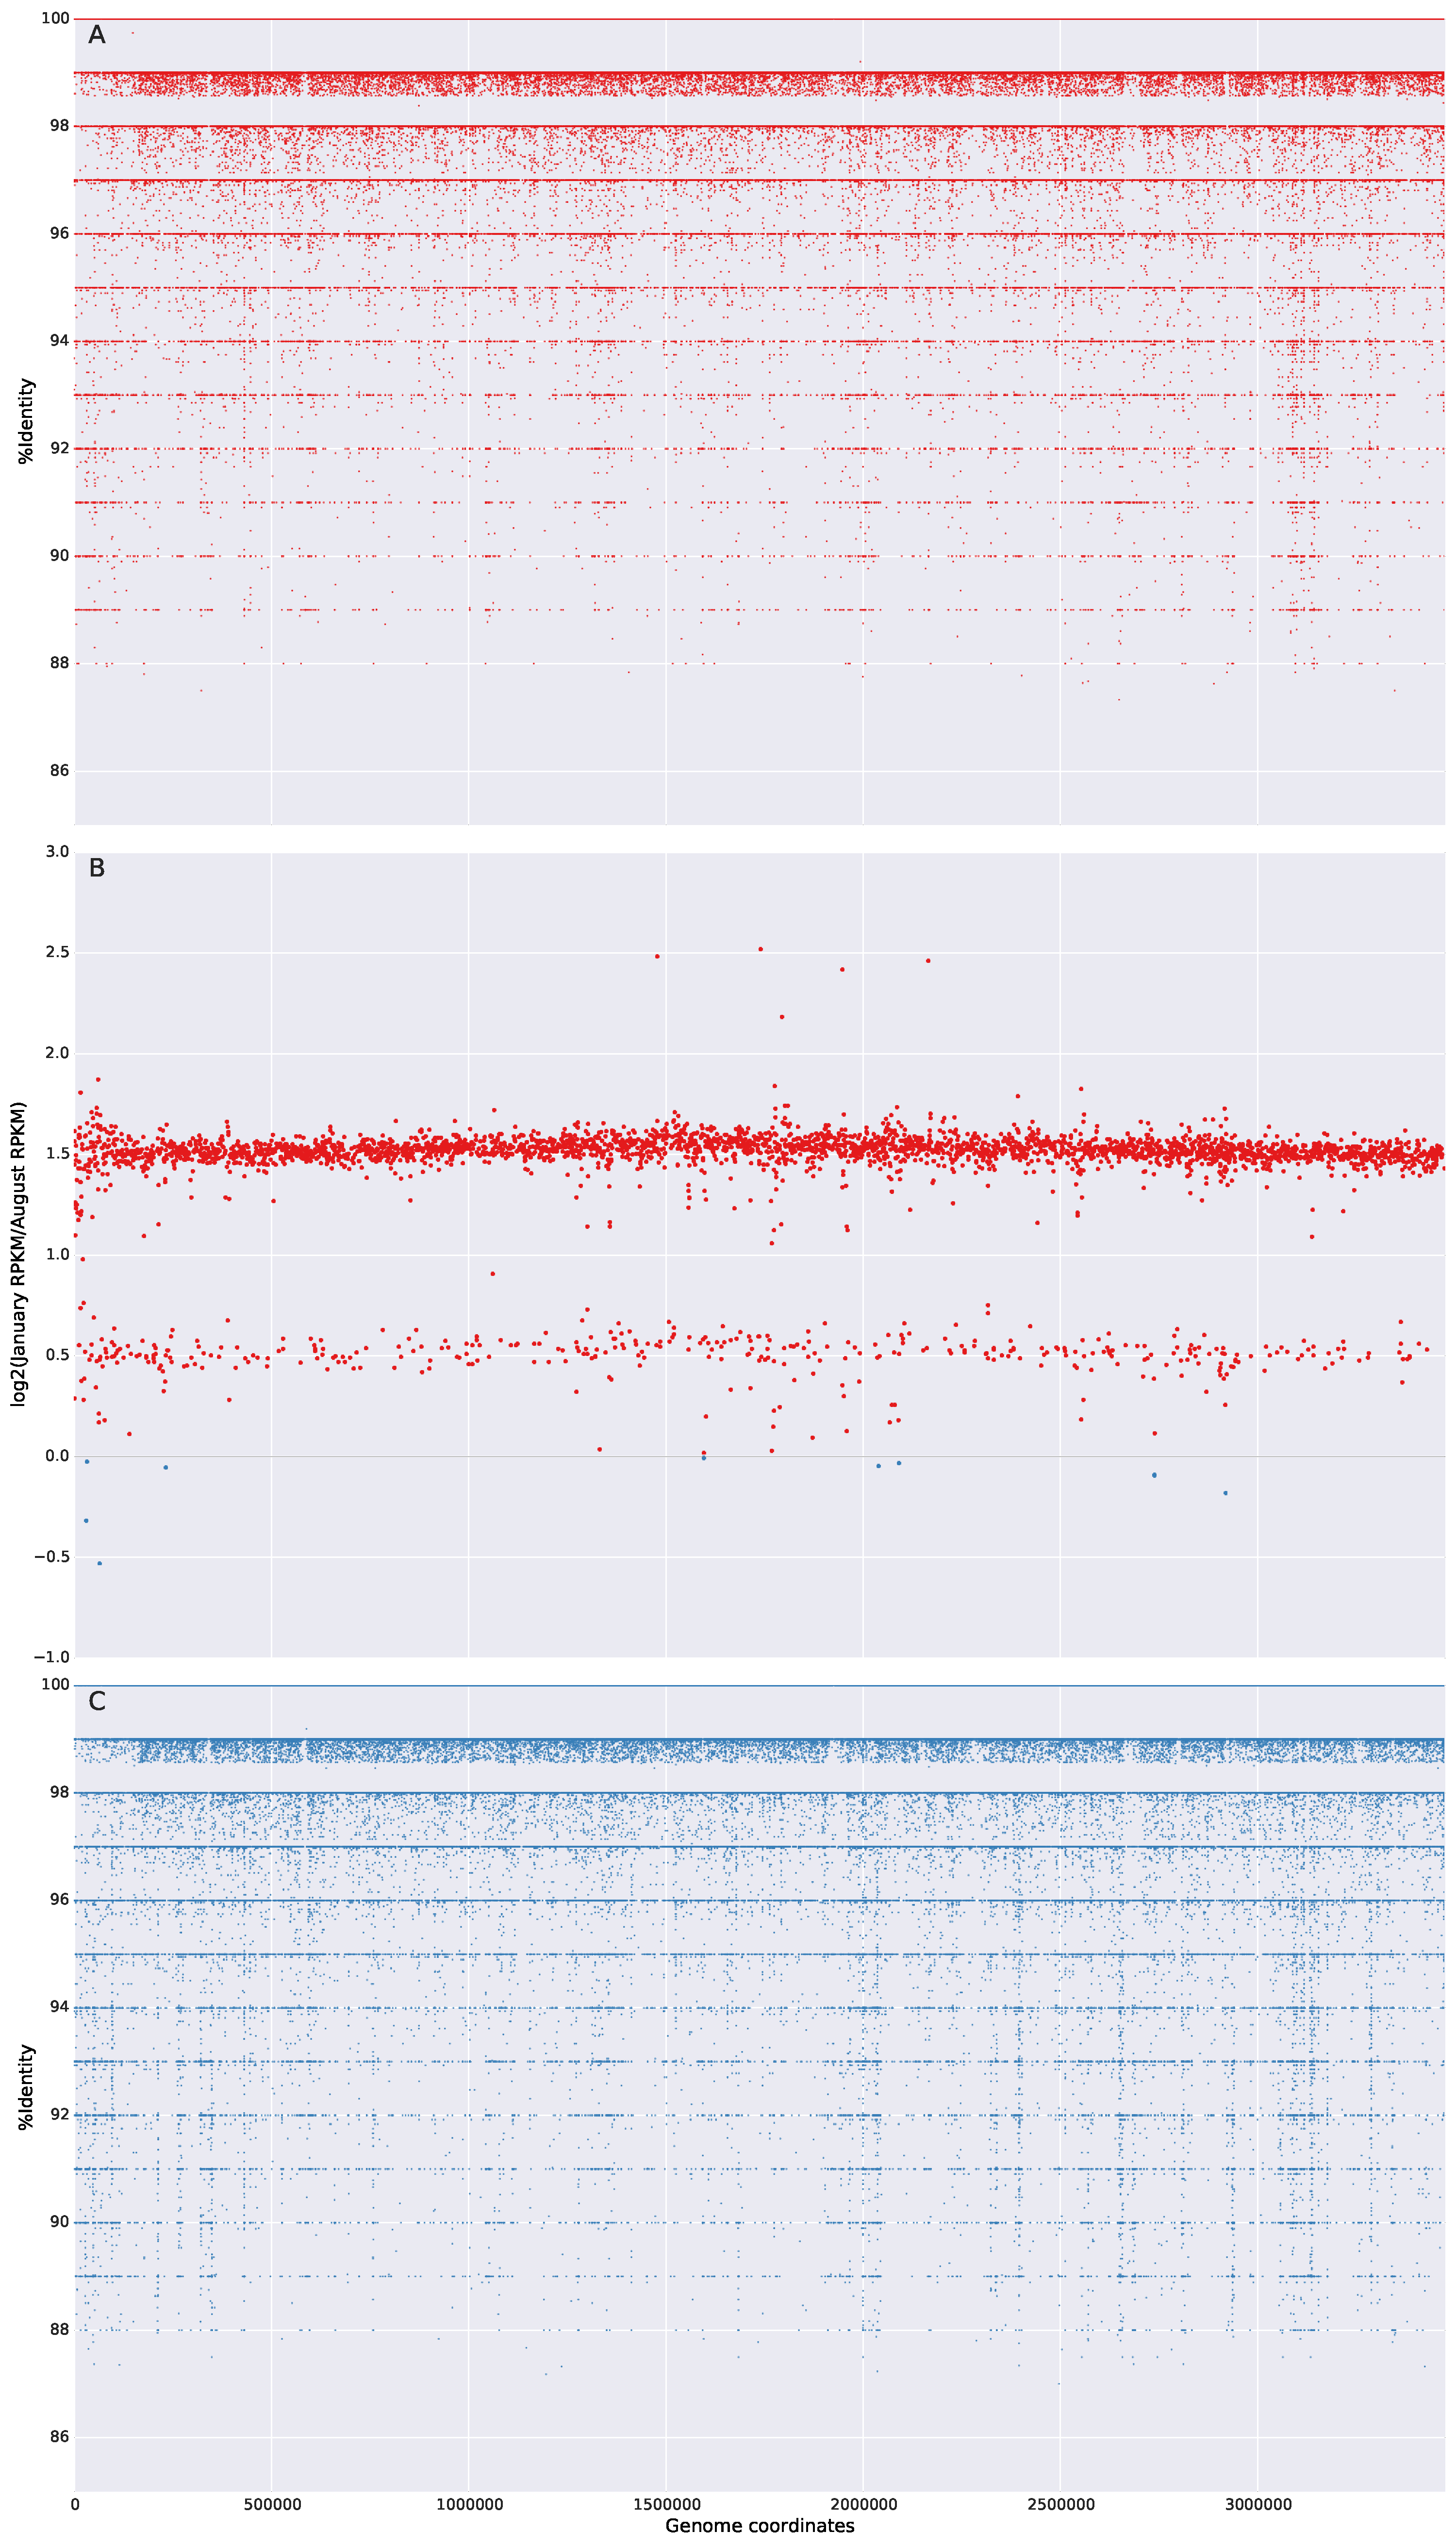
\includegraphics[width=\textwidth,height=\textheight,keepaspectratio]{Chapter5/Figures/coverage_plots/J07HWQ1_coverage.pdf}
  \caption{J07HWQ1coverage}
  \label{J07HWQ1coverage}
\end{figure}

\begin{figure}[!hbtp]
  \centering
  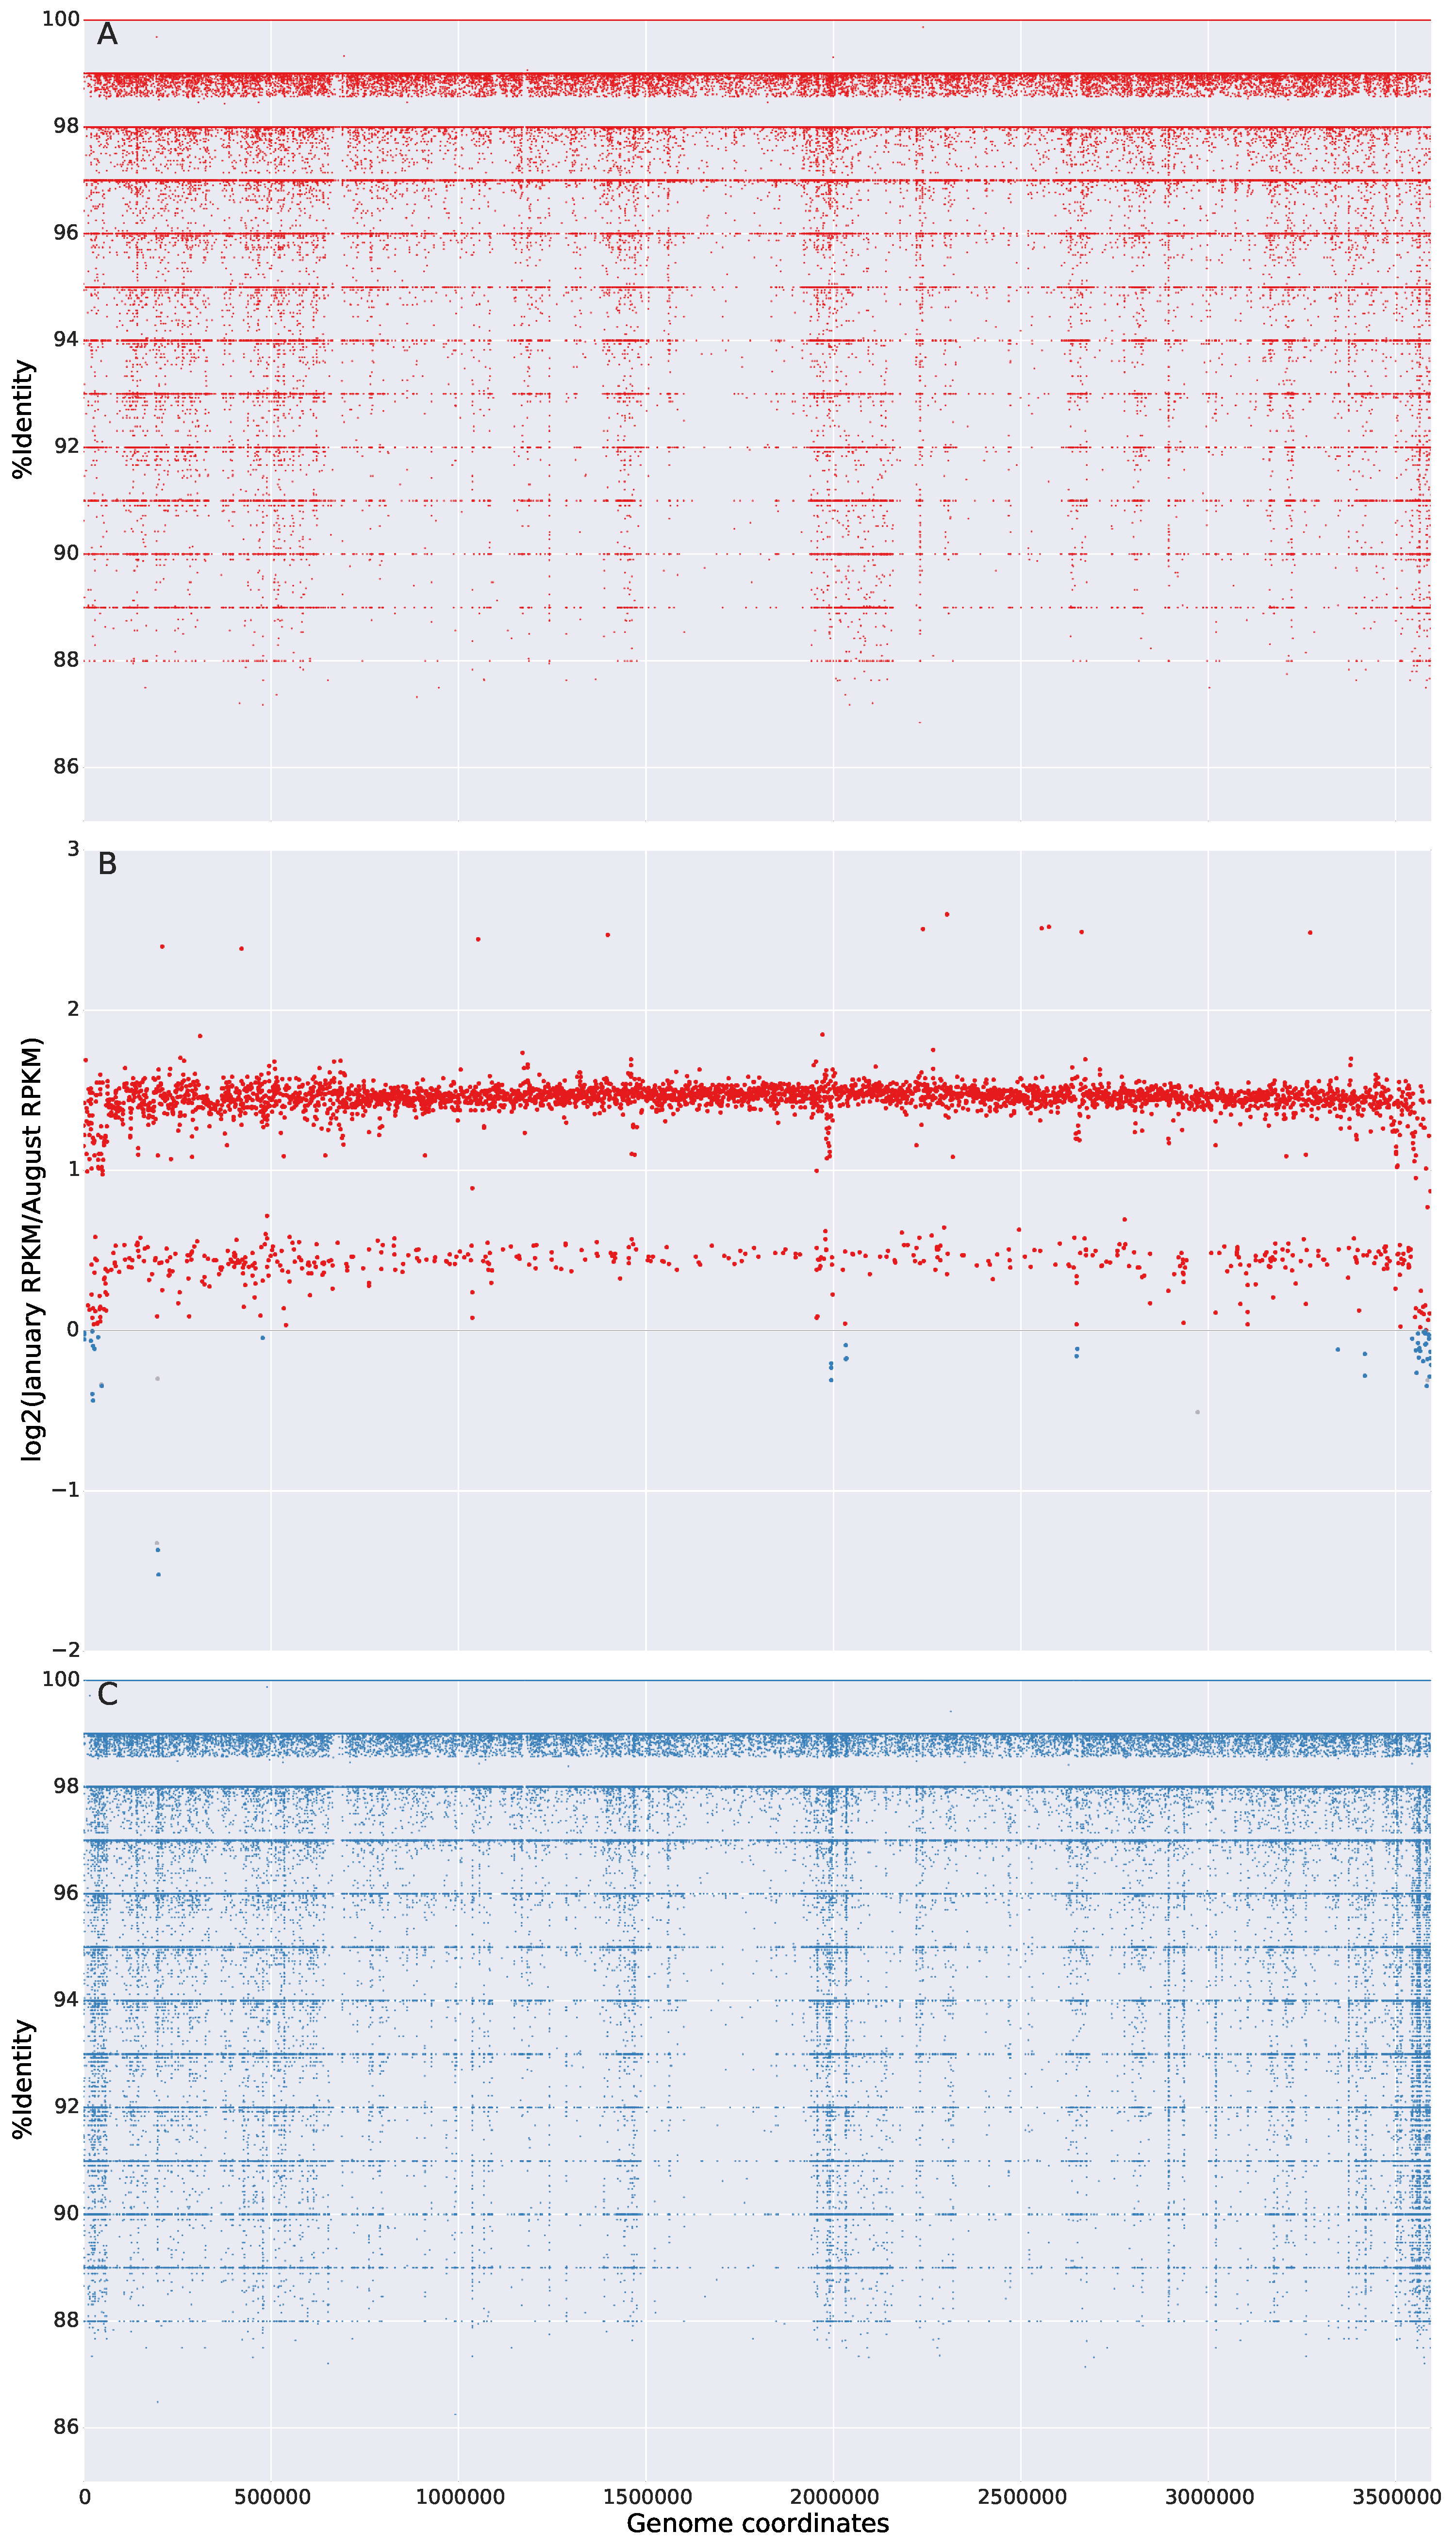
\includegraphics[width=\textwidth,height=\textheight,keepaspectratio]{Chapter5/Figures/coverage_plots/J07HWQ2_coverage.pdf}
  \caption{J07HWQ2coverage}
  \label{J07HWQ2coverage}
\end{figure}

\begin{figure}[!hbtp]
  \centering
  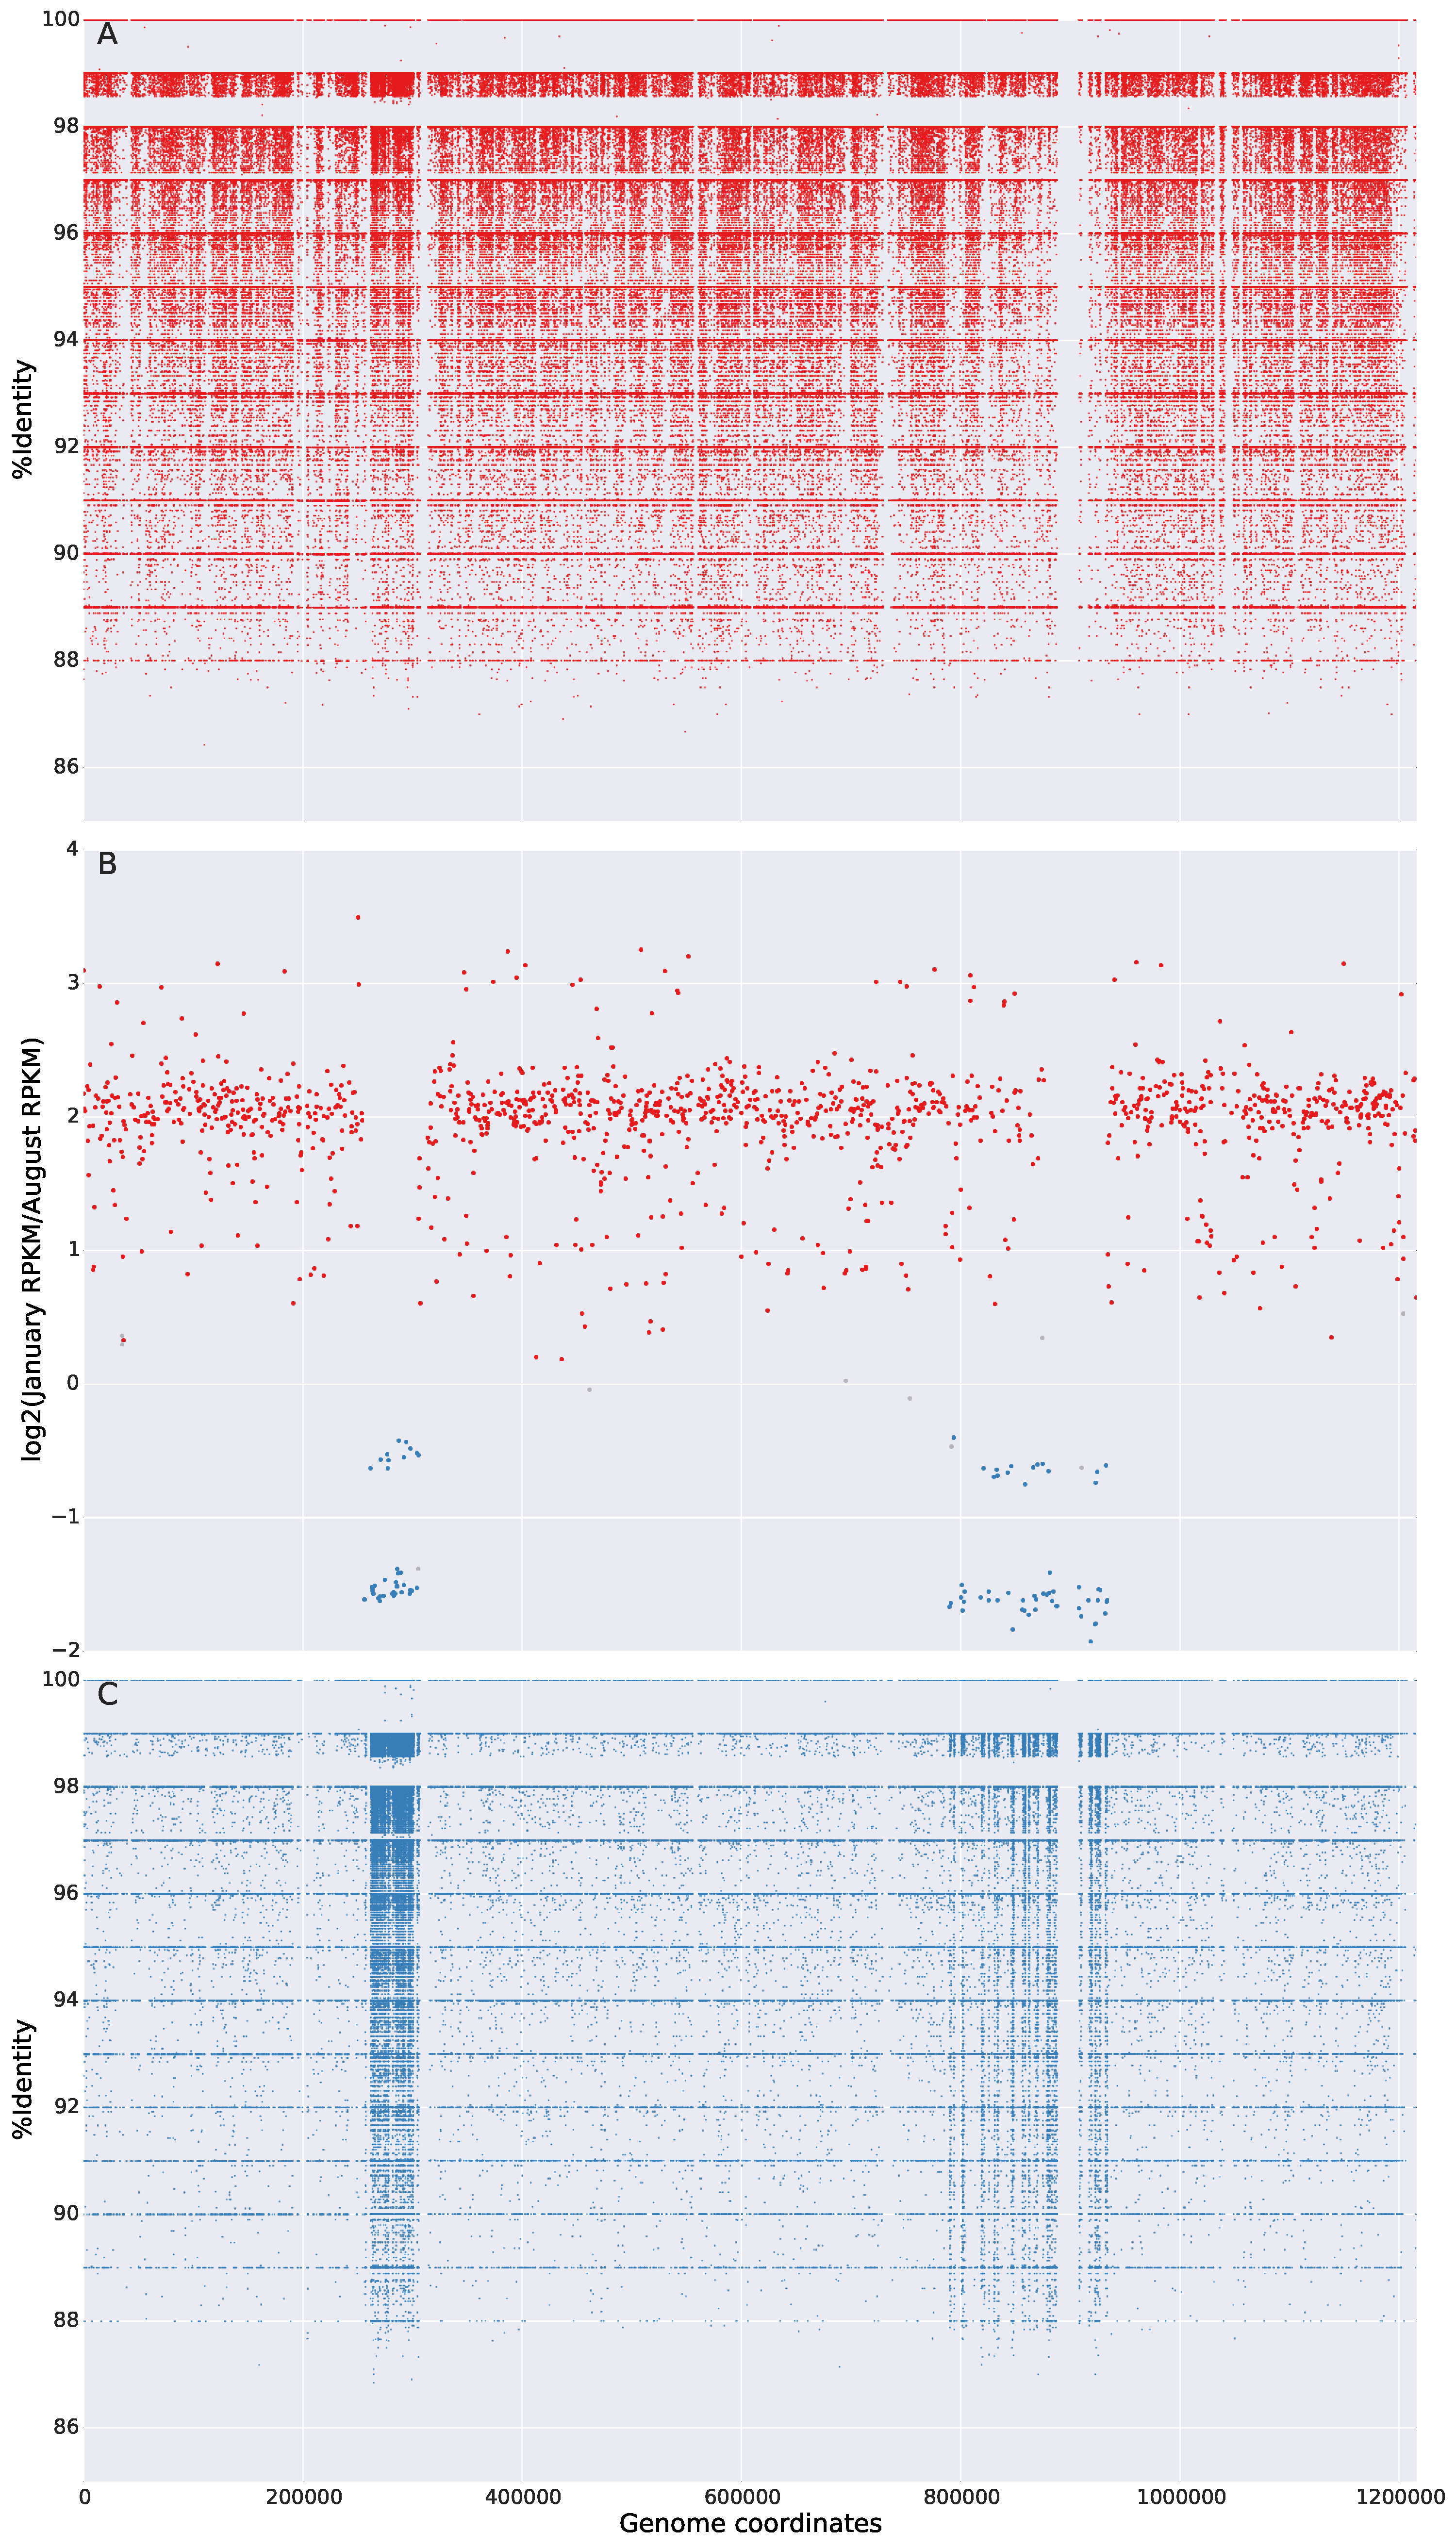
\includegraphics[width=\textwidth,height=\textheight,keepaspectratio]{Chapter5/Figures/coverage_plots/J07AB56_coverage.pdf}
  \caption{J07AB56coverage}
  \label{J07AB56coverage}
\end{figure}

\begin{figure}[!hbtp]
  \centering
  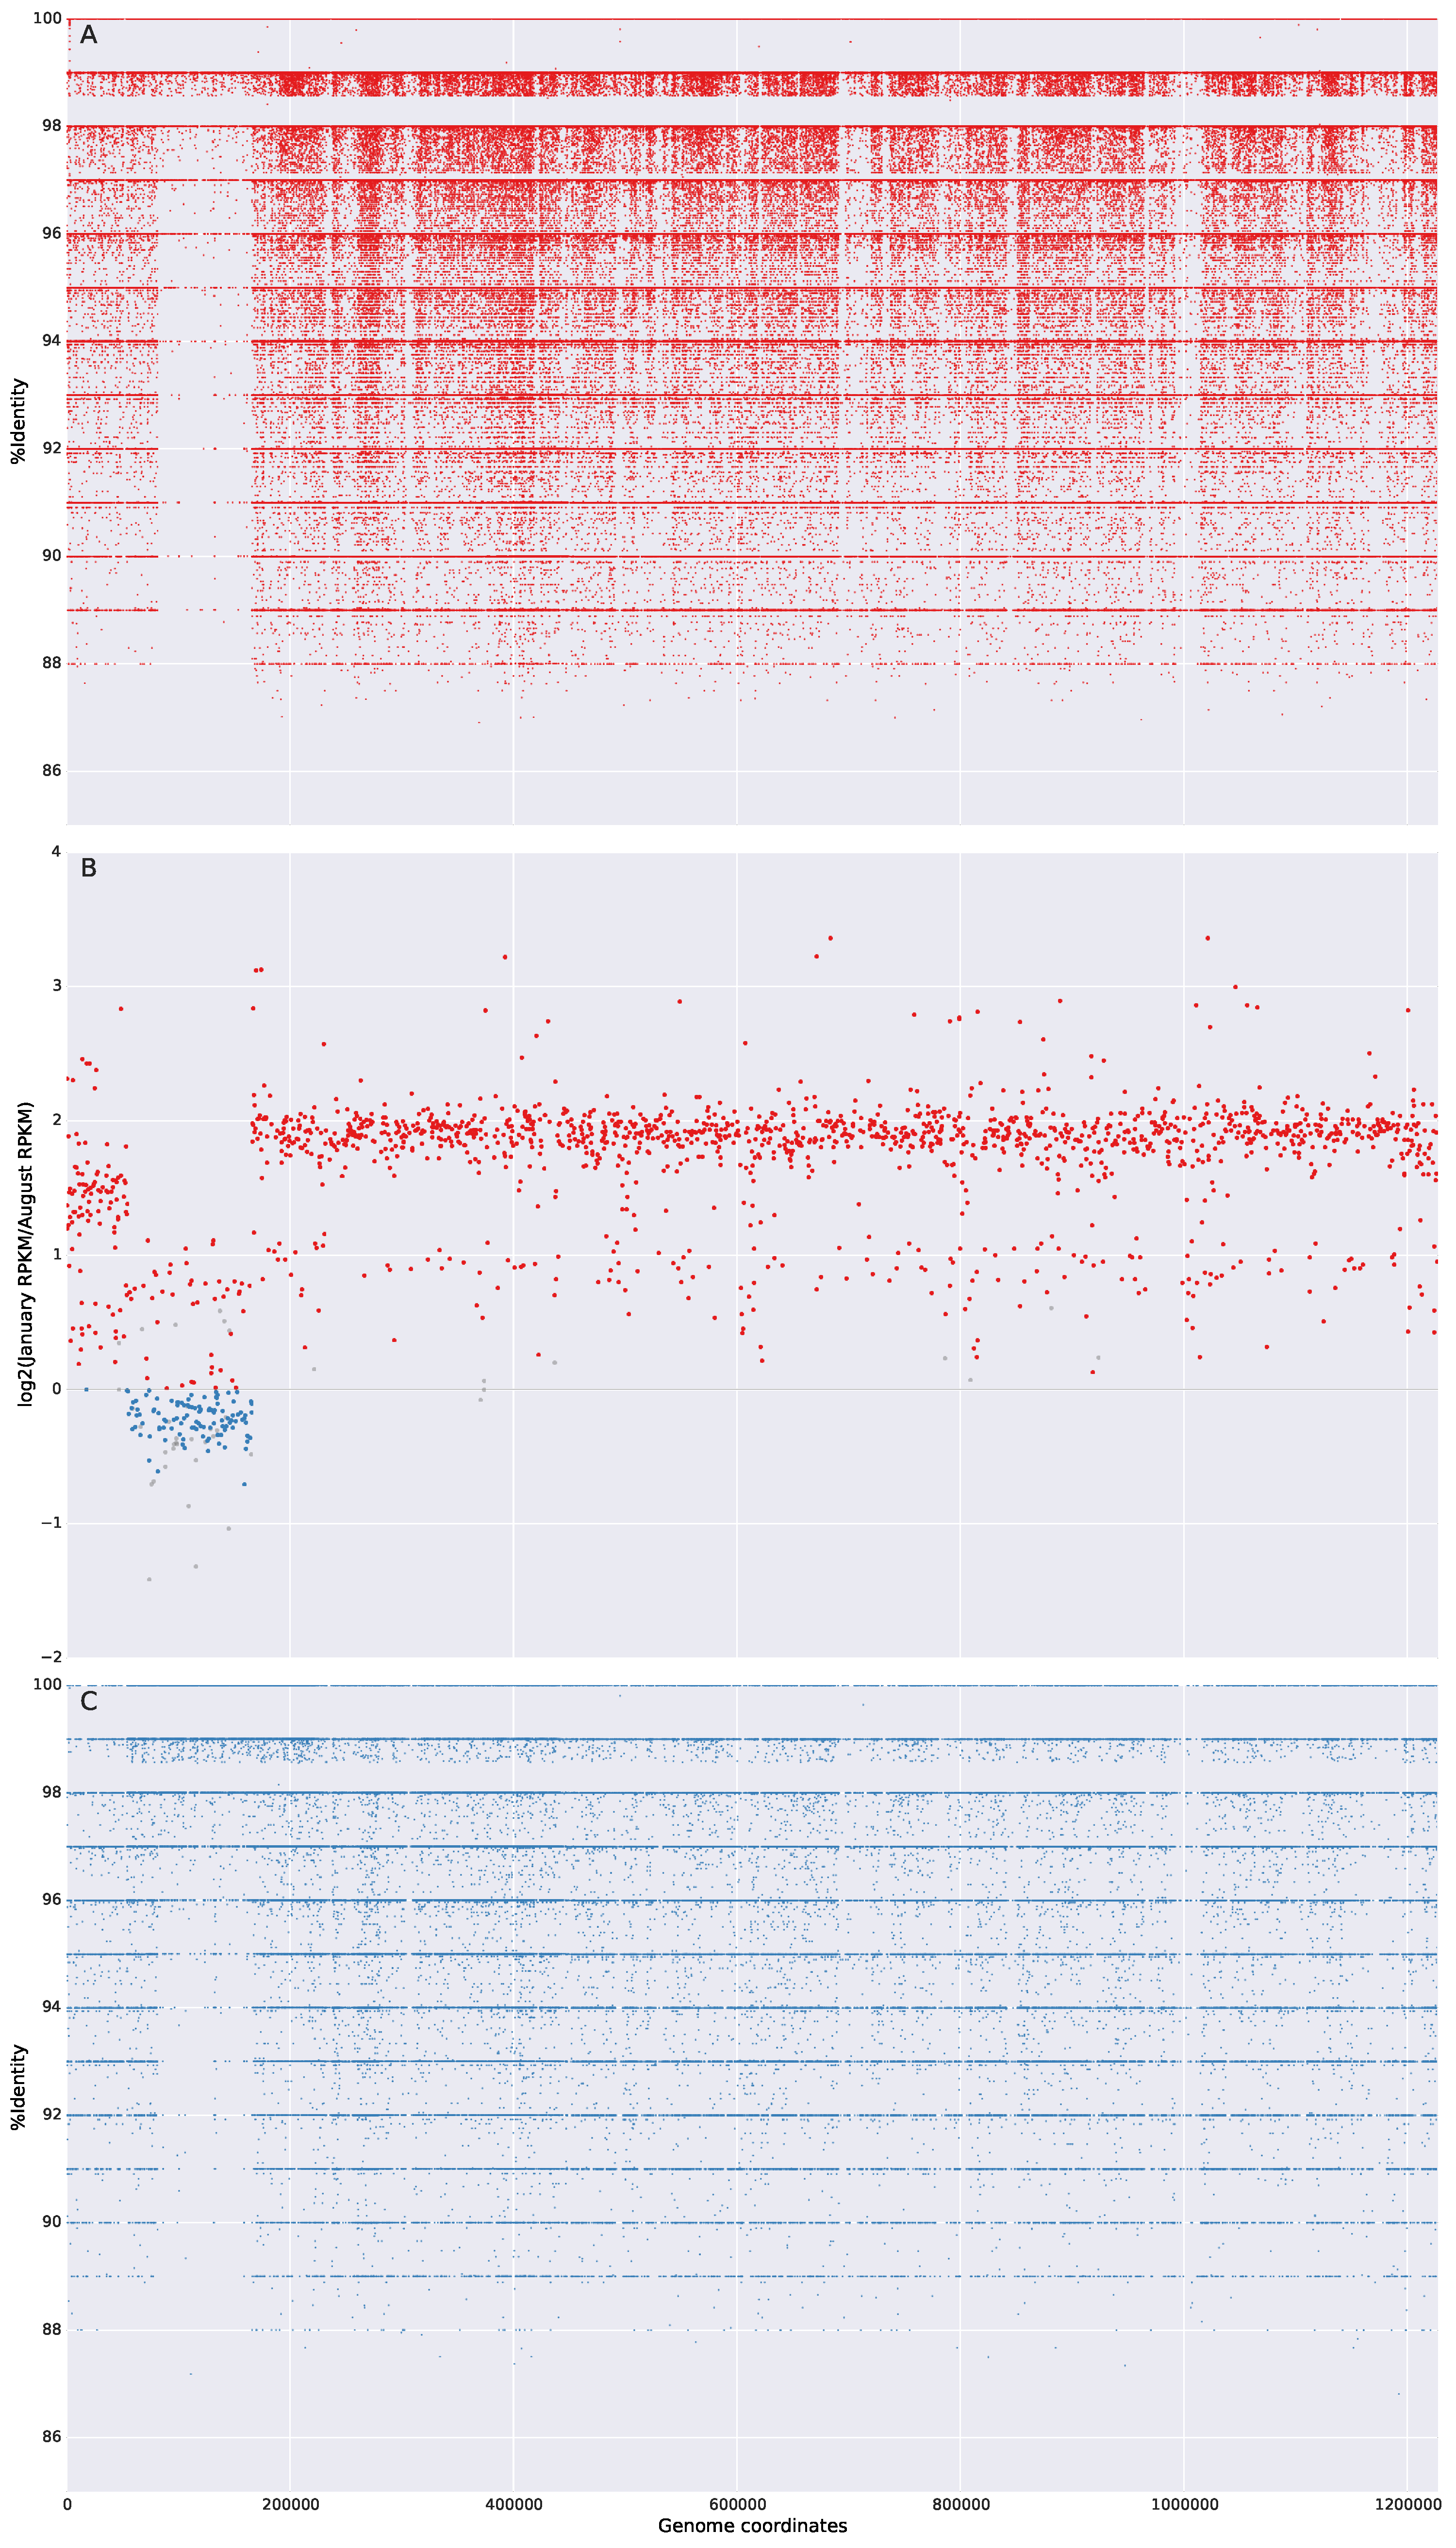
\includegraphics[width=\textwidth,height=\textheight,keepaspectratio]{Chapter5/Figures/coverage_plots/J07AB43_coverage.pdf}
  \caption{J07AB43coverage}
  \label{J07AB43ccoverage}
\end{figure}

\begin{figure}[!hbtp]
  \centering
  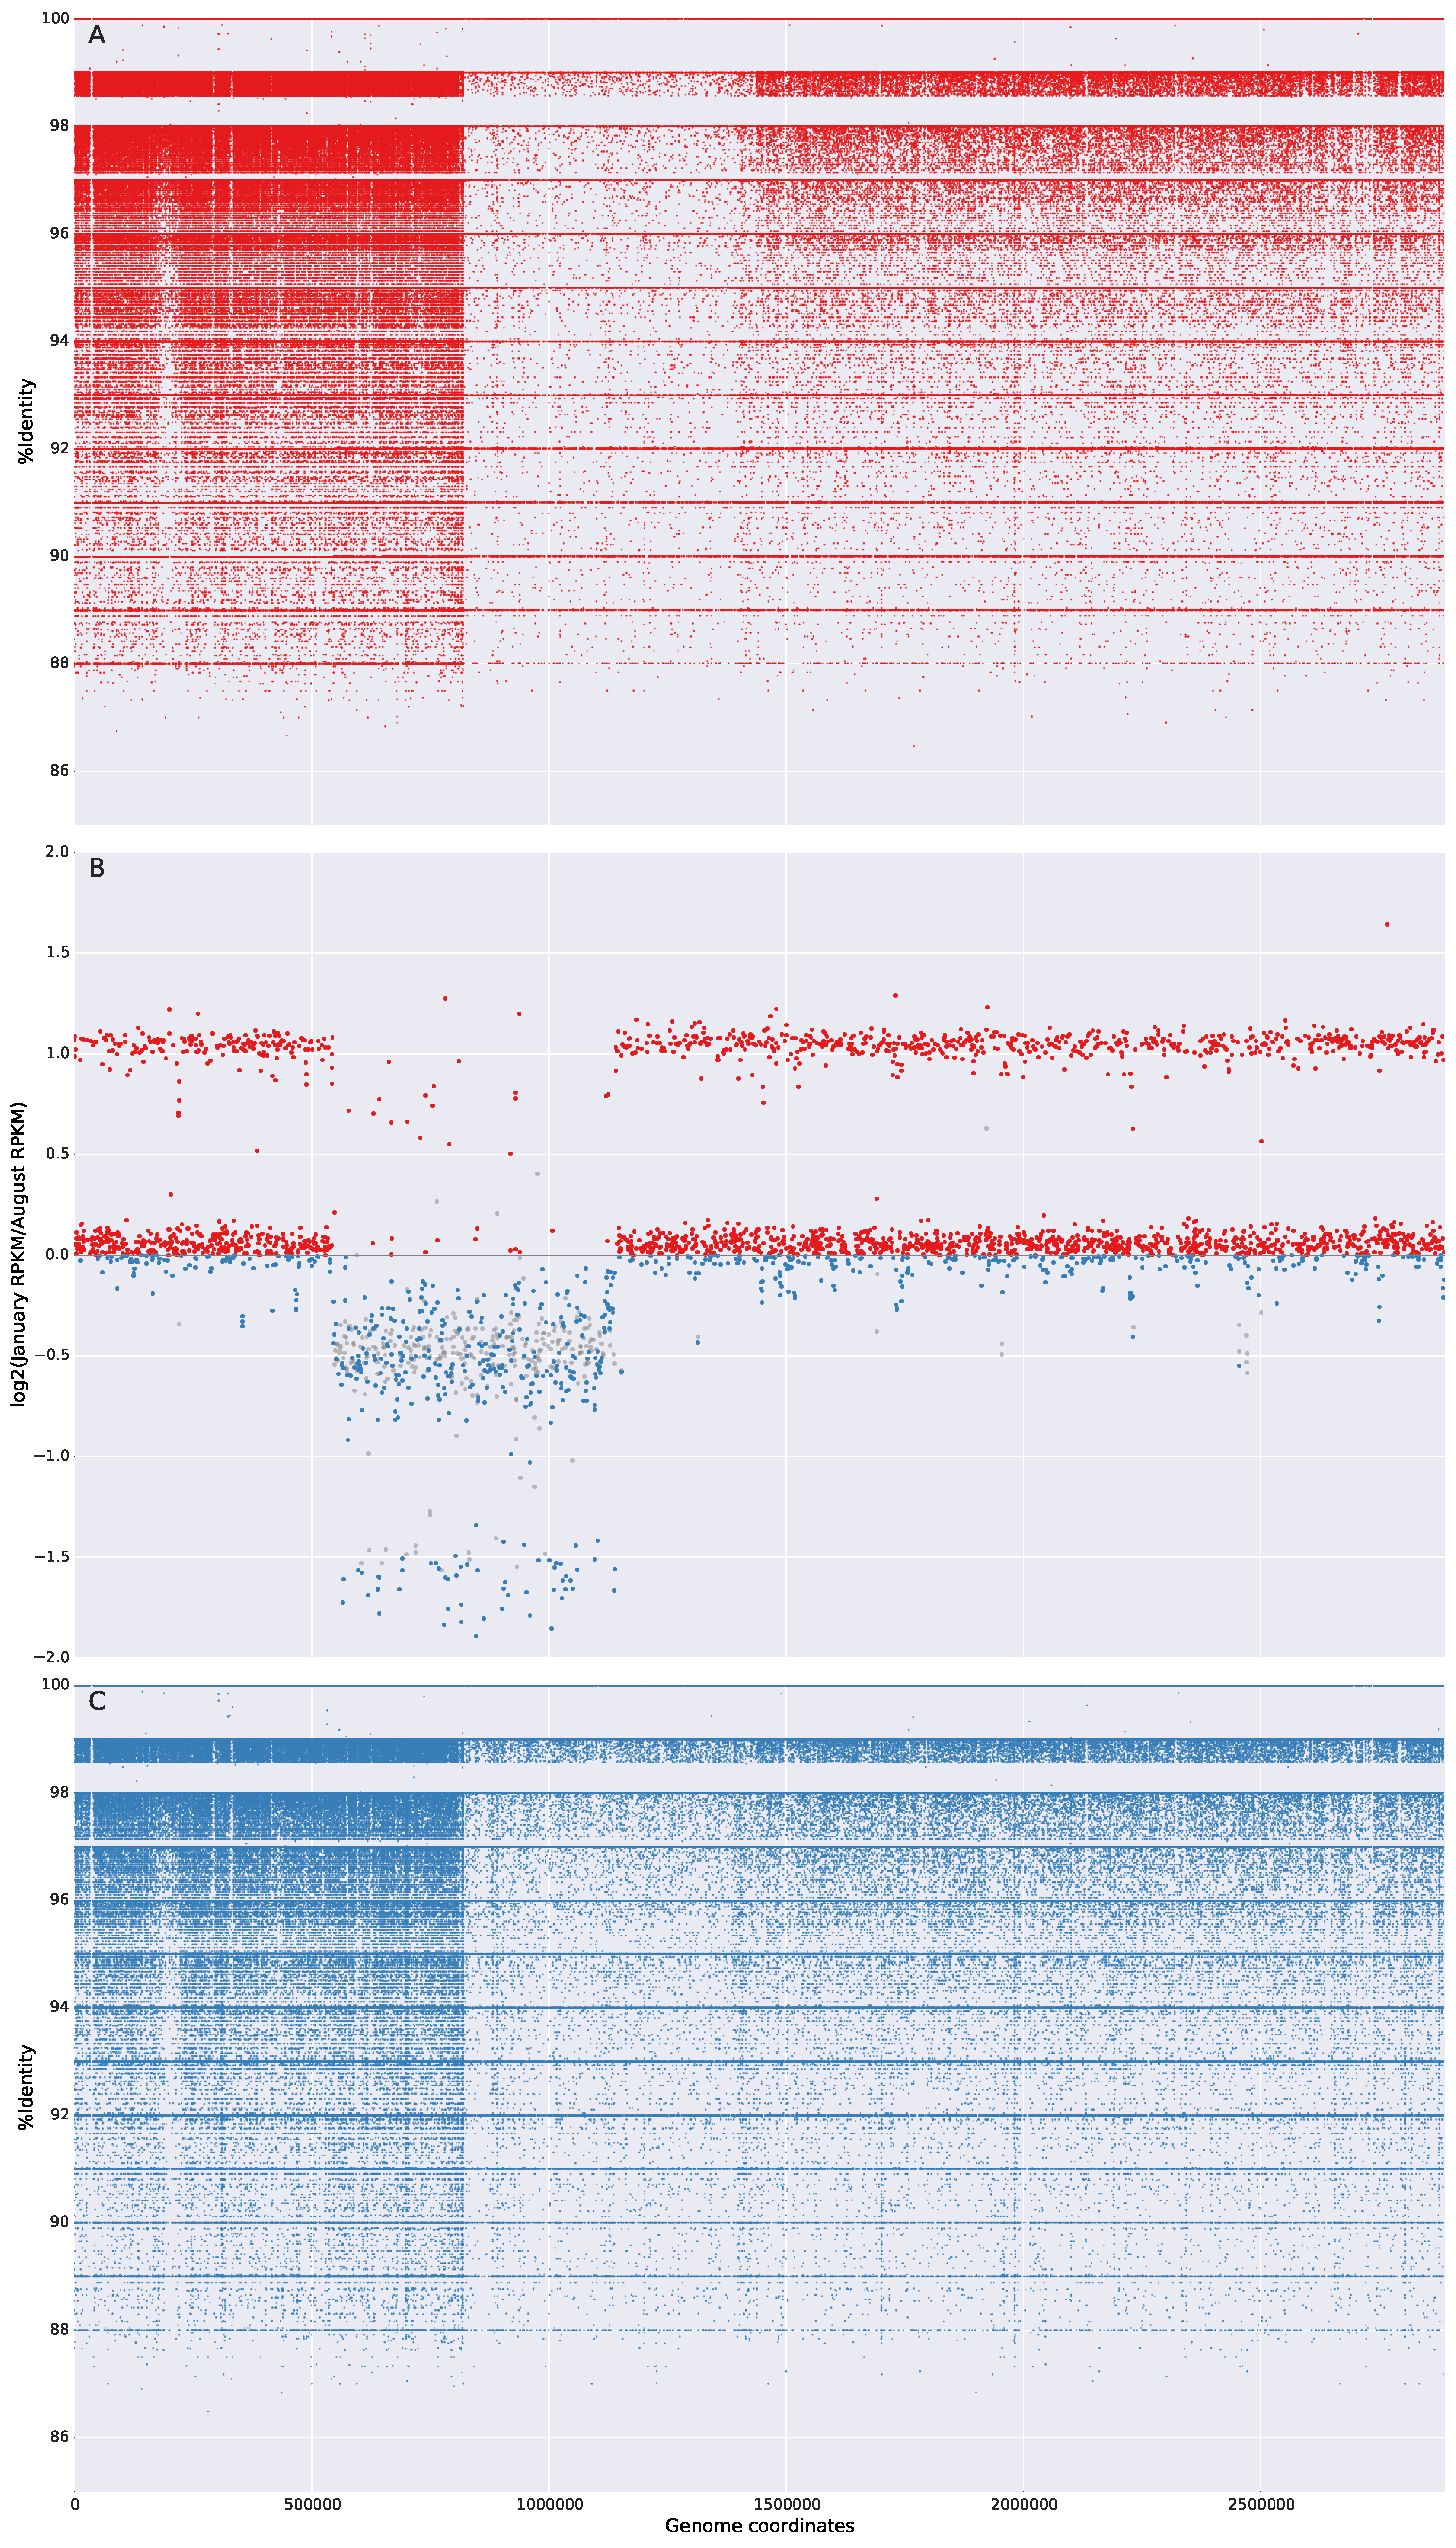
\includegraphics[width=\textwidth,height=\textheight,keepaspectratio]{Chapter5/Figures/coverage_plots/J07HN4_coverage.pdf}
  \caption{J07HN4coverage}
  \label{J07HN4coverage}
\end{figure}

\begin{figure}[!hbtp]
  \centering
  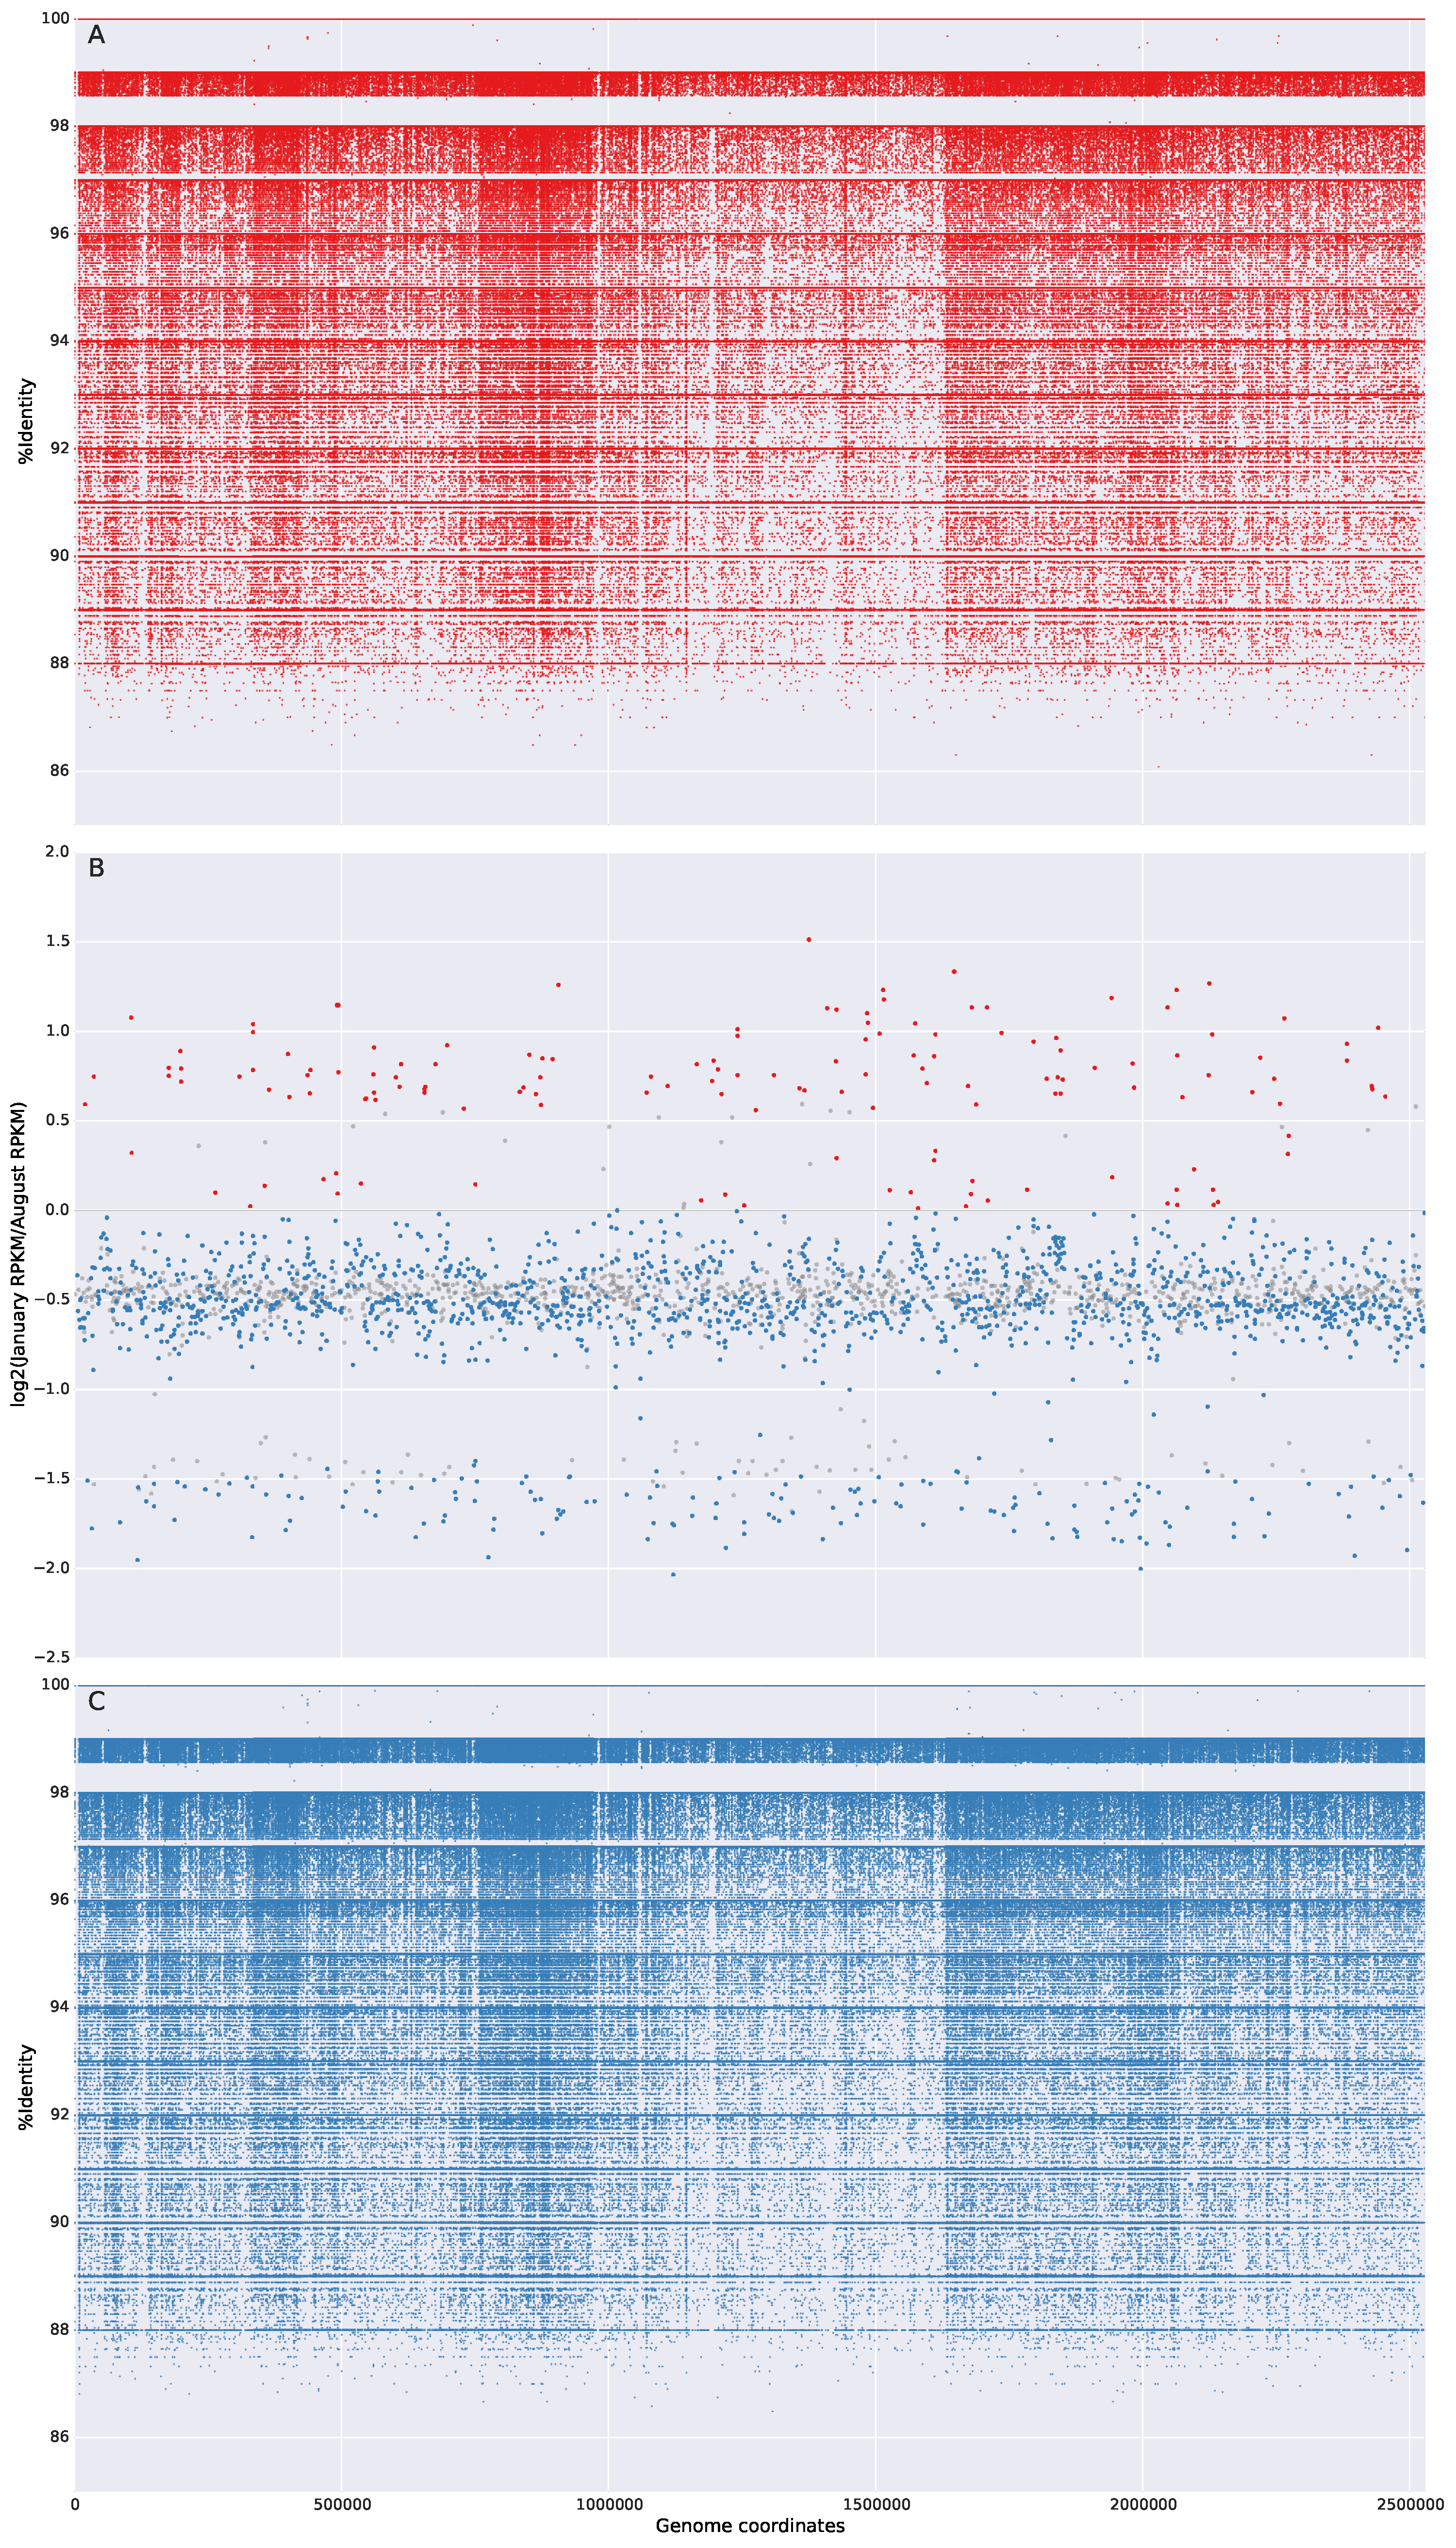
\includegraphics[width=\textwidth,height=\textheight,keepaspectratio]{Chapter5/Figures/coverage_plots/J07HN6_coverage.pdf}
  \caption{J07HN6coverage}
  \label{J07HN6coverage}
\end{figure}

\begin{figure}[!hbtp]
  \centering
  \includegraphics[width=\textwidth,height=\textheight,keepaspectratio]{Chapter5/Figures/coverage_plots/J07HX64_coverage.pdf}
  \caption{J07HN64coverage}
  \label{J07HN64coverage}
\end{figure}

\begin{figure}[!hbtp]
  \centering
  \includegraphics[width=\textwidth,height=\textheight,keepaspectratio]{Chapter5/Figures/coverage_plots/J07HX5_coverage.pdf}
  \caption{J07HX5coverage}
  \label{J07HX5coverage}
\end{figure}

\begin{figure}[!hbtp]
  \centering
  \includegraphics[width=\textwidth,height=\textheight,keepaspectratio]{Chapter5/Figures/coverage_plots/J07HB67_coverage.pdf}
  \caption{J07HB67coverage}
  \label{J07HB67coverage}
\end{figure}

\begin{figure}[!hbtp]
  \centering
  \includegraphics[width=\textwidth,height=\textheight,keepaspectratio]{Chapter5/Figures/coverage_plots/J07HR59_coverage.pdf}
  \caption{J07HR59coverage}
  \label{J07HR59coverage}
\end{figure}

\begin{figure}[!hbtp]
  \centering
  \includegraphics[width=\textwidth,height=\textheight,keepaspectratio]{Chapter5/Figures/coverage_plots/A07HB70_coverage.pdf}
  \caption{A07HB70coverage}
  \label{A07HB70coverage}
\end{figure}

\begin{figure}[!hbtp]
  \centering
  \includegraphics[width=\textwidth,height=\textheight,keepaspectratio]{Chapter5/Figures/coverage_plots/A07HR67_coverage.pdf}
  \caption{A07HR67coverage}
  \label{A07HR67coverage}
\end{figure}

\begin{figure}[!hbtp]
  \centering
  \includegraphics[width=\textwidth,height=\textheight,keepaspectratio]{Chapter5/Figures/coverage_plots/A07HN63_coverage.pdf}
  \caption{A07HN63coverage}
  \label{A07HN63coverage}
\end{figure}

\begin{figure}[!hbtp]
  \centering
  \includegraphics[width=\textwidth,height=\textheight,keepaspectratio]{Chapter5/Figures/coverage_plots/A07HR60_coverage.pdf}
  \caption{A07HR60coverage}
  \label{A07HR60coverage}
\end{figure}

\begin{figure}[!hbtp]
  \centering
  \includegraphics[width=\textwidth,height=\textheight,keepaspectratio]{Chapter5/Figures/coverage_plots/G22_coverage.pdf}
  \caption{G22 coverage}
  \label{G22coverage}
\end{figure}

\begin{figure}[!hbtp]
  \centering
  \includegraphics[width=\textwidth,height=\textheight,keepaspectratio]{Chapter5/Figures/coverage_plots/J07SB_coverage.pdf}
  \caption{J07SB coverage}
  \label{J07SBcoverage}
\end{figure}


%\chapter{}\label{ReferenceSNP_analysis}
%


% Header, overrides base

    % Make sure that the sphinx doc style knows who it inherits from.
    \def\sphinxdocclass{article}

    % Declare the document class
    \documentclass[letterpaper,10pt,english]{/Users/juan/anaconda/lib/python2.7/site-packages/sphinx/texinputs/sphinxhowto}

    % Imports
    \usepackage[utf8]{inputenc}
    \DeclareUnicodeCharacter{00A0}{\\nobreakspace}
    \usepackage[T1]{fontenc}
    \usepackage{babel}
    \usepackage{times}
    \usepackage{import}
    \usepackage[Bjarne]{/Users/juan/anaconda/lib/python2.7/site-packages/sphinx/texinputs/fncychap}
    \usepackage{longtable}
    \usepackage{/Users/juan/anaconda/lib/python2.7/site-packages/sphinx/texinputs/sphinx}
    \usepackage{multirow}

    \usepackage{amsmath}
    \usepackage{amssymb}
    \usepackage{ucs}
    \usepackage{enumerate}

    % Used to make the Input/Output rules follow around the contents.
    \usepackage{needspace}

    % Pygments requirements
    \usepackage{fancyvrb}
    \usepackage{color}
    % ansi colors additions
    \definecolor{darkgreen}{rgb}{.12,.54,.11}
    \definecolor{lightgray}{gray}{.95}
    \definecolor{brown}{rgb}{0.54,0.27,0.07}
    \definecolor{purple}{rgb}{0.5,0.0,0.5}
    \definecolor{darkgray}{gray}{0.25}
    \definecolor{lightred}{rgb}{1.0,0.39,0.28}
    \definecolor{lightgreen}{rgb}{0.48,0.99,0.0}
    \definecolor{lightblue}{rgb}{0.53,0.81,0.92}
    \definecolor{lightpurple}{rgb}{0.87,0.63,0.87}
    \definecolor{lightcyan}{rgb}{0.5,1.0,0.83}

    % Needed to box output/input
    \usepackage{tikz}
        \usetikzlibrary{calc,arrows,shadows}
    \usepackage[framemethod=tikz]{mdframed}

    \usepackage{alltt}

    % Used to load and display graphics
    \usepackage{graphicx}
    \graphicspath{ {figs/} }
    \usepackage[Export]{adjustbox} % To resize

    % used so that images for notebooks which have spaces in the name can still be included
    \usepackage{grffile}


    % For formatting output while also word wrapping.
    \usepackage{listings}
    \lstset{breaklines=true}
    \lstset{basicstyle=\small\ttfamily}
    \def\smaller{\fontsize{9.5pt}{9.5pt}\selectfont}

    %Pygments definitions
    
\makeatletter
\def\PY@reset{\let\PY@it=\relax \let\PY@bf=\relax%
    \let\PY@ul=\relax \let\PY@tc=\relax%
    \let\PY@bc=\relax \let\PY@ff=\relax}
\def\PY@tok#1{\csname PY@tok@#1\endcsname}
\def\PY@toks#1+{\ifx\relax#1\empty\else%
    \PY@tok{#1}\expandafter\PY@toks\fi}
\def\PY@do#1{\PY@bc{\PY@tc{\PY@ul{%
    \PY@it{\PY@bf{\PY@ff{#1}}}}}}}
\def\PY#1#2{\PY@reset\PY@toks#1+\relax+\PY@do{#2}}

\expandafter\def\csname PY@tok@gd\endcsname{\def\PY@tc##1{\textcolor[rgb]{0.63,0.00,0.00}{##1}}}
\expandafter\def\csname PY@tok@gu\endcsname{\let\PY@bf=\textbf\def\PY@tc##1{\textcolor[rgb]{0.50,0.00,0.50}{##1}}}
\expandafter\def\csname PY@tok@gt\endcsname{\def\PY@tc##1{\textcolor[rgb]{0.00,0.27,0.87}{##1}}}
\expandafter\def\csname PY@tok@gs\endcsname{\let\PY@bf=\textbf}
\expandafter\def\csname PY@tok@gr\endcsname{\def\PY@tc##1{\textcolor[rgb]{1.00,0.00,0.00}{##1}}}
\expandafter\def\csname PY@tok@cm\endcsname{\let\PY@it=\textit\def\PY@tc##1{\textcolor[rgb]{0.25,0.50,0.50}{##1}}}
\expandafter\def\csname PY@tok@vg\endcsname{\def\PY@tc##1{\textcolor[rgb]{0.10,0.09,0.49}{##1}}}
\expandafter\def\csname PY@tok@m\endcsname{\def\PY@tc##1{\textcolor[rgb]{0.40,0.40,0.40}{##1}}}
\expandafter\def\csname PY@tok@mh\endcsname{\def\PY@tc##1{\textcolor[rgb]{0.40,0.40,0.40}{##1}}}
\expandafter\def\csname PY@tok@go\endcsname{\def\PY@tc##1{\textcolor[rgb]{0.53,0.53,0.53}{##1}}}
\expandafter\def\csname PY@tok@ge\endcsname{\let\PY@it=\textit}
\expandafter\def\csname PY@tok@vc\endcsname{\def\PY@tc##1{\textcolor[rgb]{0.10,0.09,0.49}{##1}}}
\expandafter\def\csname PY@tok@il\endcsname{\def\PY@tc##1{\textcolor[rgb]{0.40,0.40,0.40}{##1}}}
\expandafter\def\csname PY@tok@cs\endcsname{\let\PY@it=\textit\def\PY@tc##1{\textcolor[rgb]{0.25,0.50,0.50}{##1}}}
\expandafter\def\csname PY@tok@cp\endcsname{\def\PY@tc##1{\textcolor[rgb]{0.74,0.48,0.00}{##1}}}
\expandafter\def\csname PY@tok@gi\endcsname{\def\PY@tc##1{\textcolor[rgb]{0.00,0.63,0.00}{##1}}}
\expandafter\def\csname PY@tok@gh\endcsname{\let\PY@bf=\textbf\def\PY@tc##1{\textcolor[rgb]{0.00,0.00,0.50}{##1}}}
\expandafter\def\csname PY@tok@ni\endcsname{\let\PY@bf=\textbf\def\PY@tc##1{\textcolor[rgb]{0.60,0.60,0.60}{##1}}}
\expandafter\def\csname PY@tok@nl\endcsname{\def\PY@tc##1{\textcolor[rgb]{0.63,0.63,0.00}{##1}}}
\expandafter\def\csname PY@tok@nn\endcsname{\let\PY@bf=\textbf\def\PY@tc##1{\textcolor[rgb]{0.00,0.00,1.00}{##1}}}
\expandafter\def\csname PY@tok@no\endcsname{\def\PY@tc##1{\textcolor[rgb]{0.53,0.00,0.00}{##1}}}
\expandafter\def\csname PY@tok@na\endcsname{\def\PY@tc##1{\textcolor[rgb]{0.49,0.56,0.16}{##1}}}
\expandafter\def\csname PY@tok@nb\endcsname{\def\PY@tc##1{\textcolor[rgb]{0.00,0.50,0.00}{##1}}}
\expandafter\def\csname PY@tok@nc\endcsname{\let\PY@bf=\textbf\def\PY@tc##1{\textcolor[rgb]{0.00,0.00,1.00}{##1}}}
\expandafter\def\csname PY@tok@nd\endcsname{\def\PY@tc##1{\textcolor[rgb]{0.67,0.13,1.00}{##1}}}
\expandafter\def\csname PY@tok@ne\endcsname{\let\PY@bf=\textbf\def\PY@tc##1{\textcolor[rgb]{0.82,0.25,0.23}{##1}}}
\expandafter\def\csname PY@tok@nf\endcsname{\def\PY@tc##1{\textcolor[rgb]{0.00,0.00,1.00}{##1}}}
\expandafter\def\csname PY@tok@si\endcsname{\let\PY@bf=\textbf\def\PY@tc##1{\textcolor[rgb]{0.73,0.40,0.53}{##1}}}
\expandafter\def\csname PY@tok@s2\endcsname{\def\PY@tc##1{\textcolor[rgb]{0.73,0.13,0.13}{##1}}}
\expandafter\def\csname PY@tok@vi\endcsname{\def\PY@tc##1{\textcolor[rgb]{0.10,0.09,0.49}{##1}}}
\expandafter\def\csname PY@tok@nt\endcsname{\let\PY@bf=\textbf\def\PY@tc##1{\textcolor[rgb]{0.00,0.50,0.00}{##1}}}
\expandafter\def\csname PY@tok@nv\endcsname{\def\PY@tc##1{\textcolor[rgb]{0.10,0.09,0.49}{##1}}}
\expandafter\def\csname PY@tok@s1\endcsname{\def\PY@tc##1{\textcolor[rgb]{0.73,0.13,0.13}{##1}}}
\expandafter\def\csname PY@tok@sh\endcsname{\def\PY@tc##1{\textcolor[rgb]{0.73,0.13,0.13}{##1}}}
\expandafter\def\csname PY@tok@sc\endcsname{\def\PY@tc##1{\textcolor[rgb]{0.73,0.13,0.13}{##1}}}
\expandafter\def\csname PY@tok@sx\endcsname{\def\PY@tc##1{\textcolor[rgb]{0.00,0.50,0.00}{##1}}}
\expandafter\def\csname PY@tok@bp\endcsname{\def\PY@tc##1{\textcolor[rgb]{0.00,0.50,0.00}{##1}}}
\expandafter\def\csname PY@tok@c1\endcsname{\let\PY@it=\textit\def\PY@tc##1{\textcolor[rgb]{0.25,0.50,0.50}{##1}}}
\expandafter\def\csname PY@tok@kc\endcsname{\let\PY@bf=\textbf\def\PY@tc##1{\textcolor[rgb]{0.00,0.50,0.00}{##1}}}
\expandafter\def\csname PY@tok@c\endcsname{\let\PY@it=\textit\def\PY@tc##1{\textcolor[rgb]{0.25,0.50,0.50}{##1}}}
\expandafter\def\csname PY@tok@mf\endcsname{\def\PY@tc##1{\textcolor[rgb]{0.40,0.40,0.40}{##1}}}
\expandafter\def\csname PY@tok@err\endcsname{\def\PY@bc##1{\setlength{\fboxsep}{0pt}\fcolorbox[rgb]{1.00,0.00,0.00}{1,1,1}{\strut ##1}}}
\expandafter\def\csname PY@tok@kd\endcsname{\let\PY@bf=\textbf\def\PY@tc##1{\textcolor[rgb]{0.00,0.50,0.00}{##1}}}
\expandafter\def\csname PY@tok@ss\endcsname{\def\PY@tc##1{\textcolor[rgb]{0.10,0.09,0.49}{##1}}}
\expandafter\def\csname PY@tok@sr\endcsname{\def\PY@tc##1{\textcolor[rgb]{0.73,0.40,0.53}{##1}}}
\expandafter\def\csname PY@tok@mo\endcsname{\def\PY@tc##1{\textcolor[rgb]{0.40,0.40,0.40}{##1}}}
\expandafter\def\csname PY@tok@kn\endcsname{\let\PY@bf=\textbf\def\PY@tc##1{\textcolor[rgb]{0.00,0.50,0.00}{##1}}}
\expandafter\def\csname PY@tok@mi\endcsname{\def\PY@tc##1{\textcolor[rgb]{0.40,0.40,0.40}{##1}}}
\expandafter\def\csname PY@tok@gp\endcsname{\let\PY@bf=\textbf\def\PY@tc##1{\textcolor[rgb]{0.00,0.00,0.50}{##1}}}
\expandafter\def\csname PY@tok@o\endcsname{\def\PY@tc##1{\textcolor[rgb]{0.40,0.40,0.40}{##1}}}
\expandafter\def\csname PY@tok@kr\endcsname{\let\PY@bf=\textbf\def\PY@tc##1{\textcolor[rgb]{0.00,0.50,0.00}{##1}}}
\expandafter\def\csname PY@tok@s\endcsname{\def\PY@tc##1{\textcolor[rgb]{0.73,0.13,0.13}{##1}}}
\expandafter\def\csname PY@tok@kp\endcsname{\def\PY@tc##1{\textcolor[rgb]{0.00,0.50,0.00}{##1}}}
\expandafter\def\csname PY@tok@w\endcsname{\def\PY@tc##1{\textcolor[rgb]{0.73,0.73,0.73}{##1}}}
\expandafter\def\csname PY@tok@kt\endcsname{\def\PY@tc##1{\textcolor[rgb]{0.69,0.00,0.25}{##1}}}
\expandafter\def\csname PY@tok@ow\endcsname{\let\PY@bf=\textbf\def\PY@tc##1{\textcolor[rgb]{0.67,0.13,1.00}{##1}}}
\expandafter\def\csname PY@tok@sb\endcsname{\def\PY@tc##1{\textcolor[rgb]{0.73,0.13,0.13}{##1}}}
\expandafter\def\csname PY@tok@k\endcsname{\let\PY@bf=\textbf\def\PY@tc##1{\textcolor[rgb]{0.00,0.50,0.00}{##1}}}
\expandafter\def\csname PY@tok@se\endcsname{\let\PY@bf=\textbf\def\PY@tc##1{\textcolor[rgb]{0.73,0.40,0.13}{##1}}}
\expandafter\def\csname PY@tok@sd\endcsname{\let\PY@it=\textit\def\PY@tc##1{\textcolor[rgb]{0.73,0.13,0.13}{##1}}}

\def\PYZbs{\char`\\}
\def\PYZus{\char`\_}
\def\PYZob{\char`\{}
\def\PYZcb{\char`\}}
\def\PYZca{\char`\^}
\def\PYZam{\char`\&}
\def\PYZlt{\char`\<}
\def\PYZgt{\char`\>}
\def\PYZsh{\char`\#}
\def\PYZpc{\char`\%}
\def\PYZdl{\char`\$}
\def\PYZhy{\char`\-}
\def\PYZsq{\char`\'}
\def\PYZdq{\char`\"}
\def\PYZti{\char`\~}
% for compatibility with earlier versions
\def\PYZat{@}
\def\PYZlb{[}
\def\PYZrb{]}
\makeatother


    %Set pygments styles if needed...
    
        \definecolor{nbframe-border}{rgb}{0.867,0.867,0.867}
        \definecolor{nbframe-bg}{rgb}{0.969,0.969,0.969}
        \definecolor{nbframe-in-prompt}{rgb}{0.0,0.0,0.502}
        \definecolor{nbframe-out-prompt}{rgb}{0.545,0.0,0.0}

        \newenvironment{ColorVerbatim}
        {\begin{mdframed}[%
            roundcorner=1.0pt, %
            backgroundcolor=nbframe-bg, %
            userdefinedwidth=1\linewidth, %
            leftmargin=0.1\linewidth, %
            innerleftmargin=0pt, %
            innerrightmargin=0pt, %
            linecolor=nbframe-border, %
            linewidth=1pt, %
            usetwoside=false, %
            everyline=true, %
            innerlinewidth=3pt, %
            innerlinecolor=nbframe-bg, %
            middlelinewidth=1pt, %
            middlelinecolor=nbframe-bg, %
            outerlinewidth=0.5pt, %
            outerlinecolor=nbframe-border, %
            needspace=0pt
        ]}
        {\end{mdframed}}
        
        \newenvironment{InvisibleVerbatim}
        {\begin{mdframed}[leftmargin=0.1\linewidth,innerleftmargin=3pt,innerrightmargin=3pt, userdefinedwidth=1\linewidth, linewidth=0pt, linecolor=white, usetwoside=false]}
        {\end{mdframed}}

        \renewenvironment{Verbatim}[1][\unskip]
        {\begin{alltt}\smaller}
        {\end{alltt}}
    

    % Help prevent overflowing lines due to urls and other hard-to-break 
    % entities.  This doesn't catch everything...
    \sloppy

    % Document level variables
    \title{ReferenceSNPs\_FirstStep}
    \date{March 20, 2014}
    \release{}
    \author{Unknown Author}
    \renewcommand{\releasename}{}

    % TODO: Add option for the user to specify a logo for his/her export.
    \newcommand{\sphinxlogo}{}

    % Make the index page of the document.
    \makeindex

    % Import sphinx document type specifics.
     


% Body

    % Start of the document
    \begin{document}

        
            \maketitle
        

        


        
        This notebook has the code used to process the SNP files generated by
the AMOS processes pipeline. To generate these files, the assemblies of
the J07 and A07 populations (generated using the Celera Assembler), were
proccessed using the analyzeSNPs script from AMOS.

The parameteres used for analyzeSNPs, were: - Minimum depth of 4 - At
least two different bases of consensus - Quality score of 20 or more

For those assemblies that had 454 reads, those reads were not considered
in the analysis. Only SNPs supported by Sanger reads were considered.

    % Make sure that atleast 4 lines are below the HR
    \needspace{4\baselineskip}

    
        \vspace{6pt}
        \makebox[0.1\linewidth]{\smaller\hfill\tt\color{nbframe-in-prompt}In\hspace{4pt}{[}1{]}:\hspace{4pt}}\\*
        \vspace{-2.65\baselineskip}
        \begin{ColorVerbatim}
            \vspace{-0.7\baselineskip}
            \begin{Verbatim}[commandchars=\\\{\}]
\PY{c}{\PYZsh{}Import the modules needed}
\PY{k+kn}{from} \PY{n+nn}{collections} \PY{k+kn}{import} \PY{n}{defaultdict}
\PY{k+kn}{import} \PY{n+nn}{numpy} \PY{k+kn}{as} \PY{n+nn}{np}
\PY{o}{\PYZpc{}}\PY{k}{matplotlib} \PY{n}{inline}
\PY{k+kn}{import} \PY{n+nn}{matplotlib.pyplot} \PY{k+kn}{as} \PY{n+nn}{plt}
\PY{k+kn}{import} \PY{n+nn}{matplotlib.mlab} \PY{k+kn}{as} \PY{n+nn}{mlab}
\PY{k+kn}{import} \PY{n+nn}{seaborn} \PY{k+kn}{as} \PY{n+nn}{sns}
\PY{k+kn}{from} \PY{n+nn}{collections} \PY{k+kn}{import} \PY{n}{defaultdict}
\PY{k+kn}{import} \PY{n+nn}{re}
\PY{k+kn}{from} \PY{n+nn}{Bio} \PY{k+kn}{import} \PY{n}{SeqIO}
\end{Verbatim}

            
                \vspace{-0.2\baselineskip}
            
        \end{ColorVerbatim}
    


    % Make sure that atleast 4 lines are below the HR
    \needspace{4\baselineskip}

    
        \vspace{6pt}
        \makebox[0.1\linewidth]{\smaller\hfill\tt\color{nbframe-in-prompt}In\hspace{4pt}{[}2{]}:\hspace{4pt}}\\*
        \vspace{-2.65\baselineskip}
        \begin{ColorVerbatim}
            \vspace{-0.7\baselineskip}
            \begin{Verbatim}[commandchars=\\\{\}]
\PY{c}{\PYZsh{}Read the list of scaffolds and store in a dictionary}
\PY{c}{\PYZsh{}The structure is: key\PYZhy{}\PYZgt{} Assembly\PYZus{}ID}
\PY{c}{\PYZsh{}                  values \PYZhy{}\PYZgt{} [JGI\PYZus{}ID, length]}
\PY{k}{def} \PY{n+nf}{read\PYZus{}scaffold\PYZus{}list}\PY{p}{(}\PY{n+nb}{input}\PY{p}{)}\PY{p}{:}
    
    \PY{n}{output\PYZus{}dic} \PY{o}{=} \PY{n}{defaultdict}\PY{p}{(}\PY{n+nb}{list}\PY{p}{)}
    
    \PY{k}{for} \PY{n}{line} \PY{o+ow}{in} \PY{n+nb}{open}\PY{p}{(}\PY{n+nb}{input}\PY{p}{,} \PY{l+s}{\PYZsq{}}\PY{l+s}{r}\PY{l+s}{\PYZsq{}}\PY{p}{)}\PY{p}{:}
        \PY{k}{if} \PY{n}{line}\PY{o}{.}\PY{n}{strip}\PY{p}{(}\PY{p}{)}\PY{p}{:}
            \PY{n}{line} \PY{o}{=} \PY{n}{line}\PY{o}{.}\PY{n}{rstrip}\PY{p}{(}\PY{p}{)}
            \PY{n}{info} \PY{o}{=} \PY{n}{line}\PY{o}{.}\PY{n}{split}\PY{p}{(}\PY{l+s}{\PYZdq{}}\PY{l+s+se}{\PYZbs{}t}\PY{l+s}{\PYZdq{}}\PY{p}{)}
            \PY{n}{output\PYZus{}dic}\PY{p}{[}\PY{n}{info}\PY{p}{[}\PY{l+m+mi}{0}\PY{p}{]}\PY{p}{]} \PY{o}{=} \PY{p}{[}\PY{n}{info}\PY{p}{[}\PY{l+m+mi}{2}\PY{p}{]}\PY{p}{,}\PY{n}{info}\PY{p}{[}\PY{l+m+mi}{1}\PY{p}{]}\PY{p}{]}
    
    \PY{k}{return} \PY{n}{output\PYZus{}dic}
\end{Verbatim}

            
                \vspace{-0.2\baselineskip}
            
        \end{ColorVerbatim}
    


    % Make sure that atleast 4 lines are below the HR
    \needspace{4\baselineskip}

    
        \vspace{6pt}
        \makebox[0.1\linewidth]{\smaller\hfill\tt\color{nbframe-in-prompt}In\hspace{4pt}{[}3{]}:\hspace{4pt}}\\*
        \vspace{-2.65\baselineskip}
        \begin{ColorVerbatim}
            \vspace{-0.7\baselineskip}
            \begin{Verbatim}[commandchars=\\\{\}]
\PY{c}{\PYZsh{}Read the contig\PYZhy{}scaffold mapping, store in dictionary}
\PY{c}{\PYZsh{}The structure is: key\PYZhy{}\PYZgt{}contig\PYZus{}id}
\PY{c}{\PYZsh{}Values:           values\PYZhy{}\PYZgt{}[scaf\PYZus{}id,start,end,orientation]}

\PY{k}{def} \PY{n+nf}{read\PYZus{}ctg\PYZus{}scaf\PYZus{}map}\PY{p}{(}\PY{n+nb}{input}\PY{p}{)}\PY{p}{:}
    \PY{n}{output\PYZus{}dic} \PY{o}{=} \PY{n}{defaultdict}\PY{p}{(}\PY{n+nb}{list}\PY{p}{)}
    
    \PY{k}{for} \PY{n}{line} \PY{o+ow}{in} \PY{n+nb}{open}\PY{p}{(}\PY{n+nb}{input}\PY{p}{,} \PY{l+s}{\PYZsq{}}\PY{l+s}{r}\PY{l+s}{\PYZsq{}}\PY{p}{)}\PY{p}{:}
        \PY{k}{if} \PY{n}{line}\PY{o}{.}\PY{n}{strip}\PY{p}{(}\PY{p}{)}\PY{p}{:}
            \PY{n}{line} \PY{o}{=} \PY{n}{line}\PY{o}{.}\PY{n}{rstrip}\PY{p}{(}\PY{p}{)}
            \PY{n}{info} \PY{o}{=} \PY{n}{line}\PY{o}{.}\PY{n}{split}\PY{p}{(}\PY{l+s}{\PYZdq{}}\PY{l+s+se}{\PYZbs{}t}\PY{l+s}{\PYZdq{}}\PY{p}{)}
            \PY{n}{output\PYZus{}dic}\PY{p}{[}\PY{n}{info}\PY{p}{[}\PY{l+m+mi}{0}\PY{p}{]}\PY{p}{]} \PY{o}{=} \PY{p}{[}\PY{n}{info}\PY{p}{[}\PY{l+m+mi}{1}\PY{p}{]}\PY{p}{,}\PY{n}{info}\PY{p}{[}\PY{l+m+mi}{2}\PY{p}{]}\PY{p}{,}\PY{n}{info}\PY{p}{[}\PY{l+m+mi}{3}\PY{p}{]}\PY{p}{,}\PY{n}{info}\PY{p}{[}\PY{l+m+mi}{4}\PY{p}{]}\PY{p}{]}
    
    \PY{k}{return} \PY{n}{output\PYZus{}dic}
\end{Verbatim}

            
                \vspace{-0.2\baselineskip}
            
        \end{ColorVerbatim}
    


    % Make sure that atleast 4 lines are below the HR
    \needspace{4\baselineskip}

    
        \vspace{6pt}
        \makebox[0.1\linewidth]{\smaller\hfill\tt\color{nbframe-in-prompt}In\hspace{4pt}{[}4{]}:\hspace{4pt}}\\*
        \vspace{-2.65\baselineskip}
        \begin{ColorVerbatim}
            \vspace{-0.7\baselineskip}
            \begin{Verbatim}[commandchars=\\\{\}]
\PY{c}{\PYZsh{}Read the AMOS SNP file, change info according to the scaffolds with the JGI ID and store}
\PY{c}{\PYZsh{}the information ready for the VCF file}
\PY{c}{\PYZsh{}Dictionary: key\PYZhy{}\PYZgt{}scaffold}
\PY{c}{\PYZsh{}            values: [position,id,etc..... (rest of columns VCF)}

\PY{k}{def} \PY{n+nf}{read\PYZus{}amos\PYZus{}snp}\PY{p}{(}\PY{n}{scaf\PYZus{}list}\PY{p}{,}\PY{n}{mapping}\PY{p}{,}\PY{n}{input\PYZus{}snp}\PY{p}{,}\PY{n}{genome\PYZus{}file}\PY{p}{)}\PY{p}{:}
    \PY{n}{logfile} \PY{o}{=} \PY{n+nb}{open}\PY{p}{(}\PY{l+s}{\PYZdq{}}\PY{l+s}{logfile.txt}\PY{l+s}{\PYZdq{}}\PY{p}{,} \PY{l+s}{\PYZsq{}}\PY{l+s}{w}\PY{l+s}{\PYZsq{}}\PY{p}{)}
    
    \PY{c}{\PYZsh{}Dictionary to get the complementary nucleotide}
    \PY{n}{complement\PYZus{}dict} \PY{o}{=} \PY{p}{\PYZob{}}\PY{l+s}{\PYZdq{}}\PY{l+s}{A}\PY{l+s}{\PYZdq{}}\PY{p}{:}\PY{l+s}{\PYZdq{}}\PY{l+s}{T}\PY{l+s}{\PYZdq{}}\PY{p}{,}\PY{l+s}{\PYZdq{}}\PY{l+s}{T}\PY{l+s}{\PYZdq{}}\PY{p}{:}\PY{l+s}{\PYZdq{}}\PY{l+s}{A}\PY{l+s}{\PYZdq{}}\PY{p}{,}\PY{l+s}{\PYZdq{}}\PY{l+s}{C}\PY{l+s}{\PYZdq{}}\PY{p}{:}\PY{l+s}{\PYZdq{}}\PY{l+s}{G}\PY{l+s}{\PYZdq{}}\PY{p}{,}\PY{l+s}{\PYZdq{}}\PY{l+s}{G}\PY{l+s}{\PYZdq{}}\PY{p}{:}\PY{l+s}{\PYZdq{}}\PY{l+s}{C}\PY{l+s}{\PYZdq{}}\PY{p}{\PYZcb{}}
    
    
    \PY{n}{fasta\PYZus{}sequences} \PY{o}{=} \PY{n}{SeqIO}\PY{o}{.}\PY{n}{parse}\PY{p}{(}\PY{n+nb}{open}\PY{p}{(}\PY{n}{genome\PYZus{}file}\PY{p}{)}\PY{p}{,} \PY{l+s}{\PYZdq{}}\PY{l+s}{fasta}\PY{l+s}{\PYZdq{}}\PY{p}{)}
    \PY{n}{genome\PYZus{}dictionary} \PY{o}{=} \PY{n}{defaultdict}\PY{p}{(}\PY{n+nb}{str}\PY{p}{)}
    
    \PY{k}{for} \PY{n}{fasta} \PY{o+ow}{in} \PY{n}{fasta\PYZus{}sequences}\PY{p}{:}
        \PY{n}{name}\PY{p}{,} \PY{n}{sequence} \PY{o}{=} \PY{n}{fasta}\PY{o}{.}\PY{n}{id}\PY{p}{,} \PY{n}{fasta}\PY{o}{.}\PY{n}{seq}\PY{o}{.}\PY{n}{tostring}\PY{p}{(}\PY{p}{)}
        \PY{n}{genome\PYZus{}dictionary}\PY{p}{[}\PY{n}{name}\PY{p}{]} \PY{o}{=} \PY{n}{sequence}
          
    
    \PY{n}{output\PYZus{}vcf\PYZus{}results} \PY{o}{=} \PY{n}{defaultdict}\PY{p}{(}\PY{k}{lambda}\PY{p}{:} \PY{n}{defaultdict}\PY{p}{(}\PY{n+nb}{list}\PY{p}{)}\PY{p}{)}
    \PY{n}{snp\PYZus{}count} \PY{o}{=} \PY{n}{defaultdict}\PY{p}{(}\PY{n+nb}{int}\PY{p}{)}
    
    \PY{k}{for} \PY{n}{line} \PY{o+ow}{in} \PY{n+nb}{open}\PY{p}{(}\PY{n}{input\PYZus{}snp}\PY{p}{,} \PY{l+s}{\PYZsq{}}\PY{l+s}{r}\PY{l+s}{\PYZsq{}}\PY{p}{)}\PY{p}{:}
        
        \PY{k}{if} \PY{n}{line}\PY{o}{.}\PY{n}{startswith}\PY{p}{(}\PY{l+s}{\PYZdq{}}\PY{l+s}{AsmblID}\PY{l+s}{\PYZdq{}}\PY{p}{)}\PY{p}{:}
            \PY{k}{continue}
        \PY{k}{if} \PY{n}{line}\PY{o}{.}\PY{n}{strip}\PY{p}{(}\PY{p}{)}\PY{p}{:}
            
            \PY{n}{line} \PY{o}{=} \PY{n}{line}\PY{o}{.}\PY{n}{rstrip}\PY{p}{(}\PY{p}{)}
            \PY{n}{info} \PY{o}{=} \PY{n}{line}\PY{o}{.}\PY{n}{split}\PY{p}{(}\PY{l+s}{\PYZdq{}}\PY{l+s+se}{\PYZbs{}t}\PY{l+s}{\PYZdq{}}\PY{p}{)}
            
            \PY{n}{ctg\PYZus{}id} \PY{o}{=} \PY{n}{info}\PY{p}{[}\PY{l+m+mi}{0}\PY{p}{]}
            \PY{n}{ungapped\PYZus{}position} \PY{o}{=} \PY{n}{info}\PY{p}{[}\PY{l+m+mi}{2}\PY{p}{]}
            \PY{n}{consensus\PYZus{}base} \PY{o}{=} \PY{n}{info}\PY{p}{[}\PY{l+m+mi}{3}\PY{p}{]}
            \PY{n}{depth\PYZus{}coverage} \PY{o}{=} \PY{n}{info}\PY{p}{[}\PY{l+m+mi}{4}\PY{p}{]}
            
            \PY{n}{bases\PYZus{}info} \PY{o}{=} \PY{n}{info}\PY{p}{[}\PY{l+m+mi}{6}\PY{p}{:}\PY{p}{]}
            
            \PY{c}{\PYZsh{}Skip gaps, because we are looking for SNPs, and insertion/deletions complicate the creation}
            \PY{c}{\PYZsh{}of the VCF file}
            \PY{k}{if} \PY{n}{consensus\PYZus{}base} \PY{o}{==} \PY{l+s}{\PYZdq{}}\PY{l+s}{\PYZhy{}}\PY{l+s}{\PYZdq{}}\PY{p}{:}
                \PY{k}{continue}
            
            \PY{c}{\PYZsh{}Skip if coverage is less than four:}
            \PY{k}{if} \PY{o+ow}{not} \PY{n+nb}{int}\PY{p}{(}\PY{n}{depth\PYZus{}coverage}\PY{p}{)} \PY{o}{\PYZgt{}} \PY{l+m+mi}{3}\PY{p}{:}
                \PY{k}{continue}
            
            \PY{c}{\PYZsh{}Skip those contig with no mapping info}
            \PY{k}{if} \PY{o+ow}{not} \PY{n}{ctg\PYZus{}id} \PY{o+ow}{in} \PY{n}{mapping}\PY{p}{:}
                \PY{k}{continue}
            
            
            \PY{c}{\PYZsh{}Only look at the scaffolds that are part of the assembly}
            \PY{n}{scf\PYZus{}id}\PY{p}{,}\PY{n}{start}\PY{p}{,}\PY{n}{end}\PY{p}{,}\PY{n}{orientation} \PY{o}{=} \PY{n}{mapping}\PY{p}{[}\PY{n}{ctg\PYZus{}id}\PY{p}{]}
            \PY{k}{if} \PY{o+ow}{not} \PY{n}{scf\PYZus{}id} \PY{o+ow}{in} \PY{n}{scaf\PYZus{}list}\PY{p}{:}
                \PY{k}{continue}
                
            \PY{n}{jgi\PYZus{}scf\PYZus{}id} \PY{o}{=} \PY{n}{scaf\PYZus{}list}\PY{p}{[}\PY{n}{scf\PYZus{}id}\PY{p}{]}\PY{p}{[}\PY{l+m+mi}{0}\PY{p}{]}
            
            \PY{c}{\PYZsh{}Calculate the SNP position in the scaffold}
            \PY{n}{snp\PYZus{}position\PYZus{}scf} \PY{o}{=} \PY{l+m+mi}{0}
            
            \PY{k}{if} \PY{n}{orientation} \PY{o}{==} \PY{l+s}{\PYZsq{}}\PY{l+s}{f}\PY{l+s}{\PYZsq{}}\PY{p}{:}
                \PY{n}{snp\PYZus{}position\PYZus{}scf} \PY{o}{=} \PY{n+nb}{int}\PY{p}{(}\PY{n}{start}\PY{p}{)} \PY{o}{+} \PY{n+nb}{int}\PY{p}{(}\PY{n}{ungapped\PYZus{}position}\PY{p}{)}
            
            \PY{k}{if} \PY{n}{orientation} \PY{o}{==} \PY{l+s}{\PYZsq{}}\PY{l+s}{r}\PY{l+s}{\PYZsq{}}\PY{p}{:}
                \PY{n}{snp\PYZus{}position\PYZus{}scf} \PY{o}{=} \PY{n+nb}{int}\PY{p}{(}\PY{n}{end}\PY{p}{)} \PY{o}{\PYZhy{}} \PY{n+nb}{int}\PY{p}{(}\PY{n}{ungapped\PYZus{}position}\PY{p}{)} \PY{o}{+} \PY{l+m+mi}{1}
            
            
            \PY{c}{\PYZsh{}Get the depth of each base}
            \PY{n}{bases\PYZus{}dict} \PY{o}{=} \PY{n}{defaultdict}\PY{p}{(}\PY{n+nb}{int}\PY{p}{)}
            \PY{n}{adjusted\PYZus{}depth} \PY{o}{=} \PY{l+m+mi}{0} 
            
            
            \PY{k}{for} \PY{n}{base} \PY{o+ow}{in} \PY{n}{bases\PYZus{}info}\PY{p}{:}
                \PY{n}{number\PYZus{}search} \PY{o}{=} \PY{n}{re}\PY{o}{.}\PY{n}{match}\PY{p}{(}\PY{l+s}{\PYZsq{}}\PY{l+s}{(}\PY{l+s}{\PYZbs{}}\PY{l+s}{D+)}\PY{l+s}{\PYZbs{}}\PY{l+s}{((}\PY{l+s}{\PYZbs{}}\PY{l+s}{d+)}\PY{l+s}{\PYZbs{}}\PY{l+s}{)}\PY{l+s}{\PYZsq{}}\PY{p}{,}\PY{n}{base}\PY{p}{)}
                
                \PY{k}{if} \PY{n+nb}{int}\PY{p}{(}\PY{n}{number\PYZus{}search}\PY{o}{.}\PY{n}{group}\PY{p}{(}\PY{l+m+mi}{2}\PY{p}{)}\PY{p}{)} \PY{o}{\PYZgt{}} \PY{l+m+mi}{2}\PY{p}{:}                    
                    \PY{n}{base} \PY{o}{=} \PY{n+nb}{str}\PY{p}{(}\PY{p}{)}
                    
                    \PY{k}{if} \PY{n}{orientation} \PY{o}{==} \PY{l+s}{\PYZsq{}}\PY{l+s}{r}\PY{l+s}{\PYZsq{}}\PY{p}{:}
                        
                        \PY{k}{if} \PY{n}{number\PYZus{}search}\PY{o}{.}\PY{n}{group}\PY{p}{(}\PY{l+m+mi}{1}\PY{p}{)} \PY{o+ow}{in} \PY{n}{complement\PYZus{}dict}\PY{p}{:}    
                            \PY{n}{base} \PY{o}{=} \PY{n}{complement\PYZus{}dict}\PY{p}{[}\PY{n}{number\PYZus{}search}\PY{o}{.}\PY{n}{group}\PY{p}{(}\PY{l+m+mi}{1}\PY{p}{)}\PY{p}{]}
                        \PY{k}{else}\PY{p}{:}
                            \PY{n}{base} \PY{o}{=} \PY{n}{number\PYZus{}search}\PY{o}{.}\PY{n}{group}\PY{p}{(}\PY{l+m+mi}{1}\PY{p}{)}
                    
                    \PY{k}{if} \PY{n}{orientation} \PY{o}{==} \PY{l+s}{\PYZsq{}}\PY{l+s}{f}\PY{l+s}{\PYZsq{}}\PY{p}{:}
                        \PY{n}{base} \PY{o}{=} \PY{n}{number\PYZus{}search}\PY{o}{.}\PY{n}{group}\PY{p}{(}\PY{l+m+mi}{1}\PY{p}{)}
                    
                    
                    \PY{n}{bases\PYZus{}dict}\PY{p}{[}\PY{n}{base}\PY{p}{]} \PY{o}{=} \PY{n}{number\PYZus{}search}\PY{o}{.}\PY{n}{group}\PY{p}{(}\PY{l+m+mi}{2}\PY{p}{)}
                    \PY{n}{adjusted\PYZus{}depth} \PY{o}{+}\PY{o}{=} \PY{n+nb}{int}\PY{p}{(}\PY{n}{number\PYZus{}search}\PY{o}{.}\PY{n}{group}\PY{p}{(}\PY{l+m+mi}{2}\PY{p}{)}\PY{p}{)}
                    
            \PY{n}{gap\PYZus{}counter} \PY{o}{=} \PY{l+m+mi}{0}
            \PY{k}{for} \PY{n}{base} \PY{o+ow}{in} \PY{n}{bases\PYZus{}dict}\PY{p}{:}
                \PY{k}{if} \PY{n}{base} \PY{o}{==} \PY{l+s}{\PYZdq{}}\PY{l+s}{\PYZhy{}}\PY{l+s}{\PYZdq{}}\PY{p}{:}
                    \PY{n}{gap\PYZus{}counter} \PY{o}{+}\PY{o}{=} \PY{l+m+mi}{1}
            
            \PY{k}{if} \PY{o+ow}{not} \PY{n}{gap\PYZus{}counter} \PY{o}{==} \PY{l+m+mi}{0}\PY{p}{:}
                \PY{k}{continue}
                
                    
            
            
            \PY{c}{\PYZsh{}Because some of the assemblies are based in 454 data, I need to check that the consensus}
            \PY{c}{\PYZsh{}is indeed the deepest base. If not, I just move to the next one. }
            \PY{c}{\PYZsh{}This is stringent, but the idea is to look at SNPs that are supported by the sanger reads}
            \PY{c}{\PYZsh{}The details of the population structure should come out from the Illumina reads}
         
            \PY{k}{if} \PY{o+ow}{not} \PY{n+nb}{len}\PY{p}{(}\PY{n}{bases\PYZus{}dict}\PY{o}{.}\PY{n}{keys}\PY{p}{(}\PY{p}{)}\PY{p}{)} \PY{o}{\PYZgt{}} \PY{l+m+mi}{1}\PY{p}{:}
                \PY{k}{continue}
            
    

            \PY{c}{\PYZsh{}Values for the final dictionary}
            \PY{c}{\PYZsh{}Chrom}
            \PY{c}{\PYZsh{}Pos}
            \PY{c}{\PYZsh{}ID, always .}
            \PY{c}{\PYZsh{}REF}
            \PY{c}{\PYZsh{}ALT If multiple, separated by , Replace \PYZdq{}\PYZhy{}\PYZdq{} with \PYZdq{}.\PYZdq{}}
            \PY{c}{\PYZsh{}Qual, always 20}
            \PY{c}{\PYZsh{}Filter, always PASS}
            \PY{c}{\PYZsh{}INFO: \PYZsh{}NS=1,DP=depth,AF=allele frequency}
            
            \PY{c}{\PYZsh{}For some reason, AMOS gives position that are not the ones found in the consensus}
            \PY{c}{\PYZsh{}Here I will check against the fasta file for the sequence, to see if the position correspond to the consensus}
            \PY{c}{\PYZsh{}or the alternates}
            
            
                        
            \PY{c}{\PYZsh{}Create the alt and allele frequency values}
            \PY{c}{\PYZsh{}genome\PYZus{}reference\PYZus{}nuc = genome\PYZus{}sequence[jgi\PYZus{}scf\PYZus{}id].seq[int(snp\PYZus{}position\PYZus{}scf) + 1]}
            \PY{n}{reference\PYZus{}position} \PY{o}{=} \PY{n+nb}{int}\PY{p}{(}\PY{n}{snp\PYZus{}position\PYZus{}scf}\PY{p}{)} \PY{o}{\PYZhy{}} \PY{l+m+mi}{1}
            
            \PY{k}{try}\PY{p}{:}
                \PY{n}{genome\PYZus{}reference\PYZus{}nuc} \PY{o}{=} \PY{n}{genome\PYZus{}dictionary}\PY{p}{[}\PY{n}{jgi\PYZus{}scf\PYZus{}id}\PY{p}{]}\PY{p}{[}\PY{n}{reference\PYZus{}position}\PY{p}{]}
            \PY{k}{except} \PY{n+ne}{IndexError}\PY{p}{:}
                \PY{n}{logfile}\PY{o}{.}\PY{n}{write}\PY{p}{(}\PY{l+s}{\PYZdq{}}\PY{l+s}{Error: }\PY{l+s+si}{\PYZpc{}s}\PY{l+s+se}{\PYZbs{}t}\PY{l+s+si}{\PYZpc{}d}\PY{l+s+se}{\PYZbs{}n}\PY{l+s}{\PYZdq{}} \PY{o}{\PYZpc{}}\PY{p}{(}\PY{n}{jgi\PYZus{}scf\PYZus{}id}\PY{p}{,}\PY{n}{reference\PYZus{}position}\PY{p}{)}\PY{p}{)}
                \PY{k}{continue}
                
            \PY{n}{new\PYZus{}reference\PYZus{}position} \PY{o}{=} \PY{l+s}{\PYZdq{}}\PY{l+s}{.}\PY{l+s}{\PYZdq{}}
            \PY{n}{alternative\PYZus{}bases} \PY{o}{=} \PY{p}{[}\PY{p}{]}
            \PY{n}{allele\PYZus{}frequency} \PY{o}{=} \PY{p}{[}\PY{p}{]}
            
            
            \PY{k}{for} \PY{n}{entry} \PY{o+ow}{in} \PY{n}{bases\PYZus{}dict}\PY{o}{.}\PY{n}{keys}\PY{p}{(}\PY{p}{)}\PY{p}{:}
                
                \PY{k}{if} \PY{n}{entry} \PY{o}{==} \PY{n}{genome\PYZus{}reference\PYZus{}nuc}\PY{p}{:}
                    \PY{n}{new\PYZus{}reference\PYZus{}position} \PY{o}{=} \PY{n}{entry}
                    
                \PY{k}{else}\PY{p}{:}
                    \PY{n}{alternative\PYZus{}bases}\PY{o}{.}\PY{n}{append}\PY{p}{(}\PY{n}{entry}\PY{p}{)}
                    \PY{n}{freq} \PY{o}{=} \PY{n+nb}{int}\PY{p}{(}\PY{n}{bases\PYZus{}dict}\PY{p}{[}\PY{n}{entry}\PY{p}{]}\PY{p}{)} \PY{o}{/} \PY{n+nb}{float}\PY{p}{(}\PY{n}{adjusted\PYZus{}depth}\PY{p}{)}
                    \PY{n}{allele\PYZus{}frequency}\PY{o}{.}\PY{n}{append}\PY{p}{(}\PY{n}{freq}\PY{p}{)}
            
            \PY{c}{\PYZsh{}Now save everything into an entry}
            
            \PY{n}{vcf\PYZus{}alt} \PY{o}{=} \PY{l+s}{\PYZdq{}}\PY{l+s}{,}\PY{l+s}{\PYZdq{}}\PY{o}{.}\PY{n}{join}\PY{p}{(}\PY{n}{alternative\PYZus{}bases}\PY{p}{)}
            \PY{n}{info\PYZus{}entry} \PY{o}{=} \PY{l+s}{\PYZdq{}}\PY{l+s}{NS=1,}\PY{l+s}{\PYZdq{}} \PY{o}{+} \PY{l+s}{\PYZdq{}}\PY{l+s}{DP=}\PY{l+s}{\PYZdq{}} \PY{o}{+} \PY{n+nb}{str}\PY{p}{(}\PY{n}{adjusted\PYZus{}depth}\PY{p}{)} \PY{o}{+} \PY{l+s}{\PYZdq{}}\PY{l+s}{,AF=}\PY{l+s}{\PYZdq{}} \PY{o}{+} \PY{l+s}{\PYZdq{}}\PY{l+s}{,}\PY{l+s}{\PYZdq{}}\PY{o}{.}\PY{n}{join}\PY{p}{(}\PY{n+nb}{map}\PY{p}{(}\PY{n+nb}{str}\PY{p}{,} \PY{n}{allele\PYZus{}frequency}\PY{p}{)}\PY{p}{)}
            
            \PY{c}{\PYZsh{}Modify consensus base to \PYZdq{}.\PYZdq{}}
            \PY{c}{\PYZsh{}if consensus\PYZus{}base == \PYZdq{}\PYZhy{}\PYZdq{}:}
            \PY{c}{\PYZsh{}    consensus\PYZus{}base = \PYZdq{}.\PYZdq{}}
            
            \PY{n}{vcf\PYZus{}entry} \PY{o}{=} \PY{p}{[}\PY{l+s}{\PYZdq{}}\PY{l+s}{.}\PY{l+s}{\PYZdq{}}\PY{p}{,} \PY{n}{new\PYZus{}reference\PYZus{}position}\PY{p}{,} \PY{n}{vcf\PYZus{}alt}\PY{p}{,} \PY{l+s}{\PYZdq{}}\PY{l+s}{20}\PY{l+s}{\PYZdq{}}\PY{p}{,} \PY{l+s}{\PYZdq{}}\PY{l+s}{PASS}\PY{l+s}{\PYZdq{}}\PY{p}{,} \PY{n}{info\PYZus{}entry}\PY{p}{]}
            
            \PY{n}{snp\PYZus{}count}\PY{p}{[}\PY{n}{scf\PYZus{}id}\PY{p}{]} \PY{o}{+}\PY{o}{=} \PY{l+m+mi}{1}
            
            \PY{n}{output\PYZus{}vcf\PYZus{}results}\PY{p}{[}\PY{n}{jgi\PYZus{}scf\PYZus{}id}\PY{p}{]}\PY{p}{[}\PY{n}{snp\PYZus{}position\PYZus{}scf}\PY{p}{]} \PY{o}{=} \PY{n}{vcf\PYZus{}entry}
            
            \PY{n}{logfile}\PY{o}{.}\PY{n}{write}\PY{p}{(}\PY{n}{orientation} \PY{o}{+} \PY{l+s}{\PYZdq{}}\PY{l+s+se}{\PYZbs{}t}\PY{l+s}{\PYZdq{}} \PY{o}{+} \PY{l+s}{\PYZdq{}}\PY{l+s}{,}\PY{l+s}{\PYZdq{}}\PY{o}{.}\PY{n}{join}\PY{p}{(}\PY{n}{bases\PYZus{}dict}\PY{o}{.}\PY{n}{keys}\PY{p}{(}\PY{p}{)}\PY{p}{)} \PY{o}{+} \PY{l+s}{\PYZdq{}}\PY{l+s+se}{\PYZbs{}t}\PY{l+s}{\PYZdq{}} \PY{o}{+} \PY{n}{genome\PYZus{}reference\PYZus{}nuc} \PY{o}{+} \PY{l+s}{\PYZdq{}}\PY{l+s}{,}\PY{l+s}{\PYZdq{}} \PY{o}{+} \PY{n}{new\PYZus{}reference\PYZus{}position} \PY{o}{+}\PY{l+s}{\PYZdq{}}\PY{l+s+se}{\PYZbs{}t}\PY{l+s}{\PYZdq{}} \PY{o}{+} \PY{n}{jgi\PYZus{}scf\PYZus{}id} \PY{o}{+}\PY{l+s}{\PYZdq{}}\PY{l+s+se}{\PYZbs{}t}\PY{l+s}{\PYZdq{}} \PY{o}{+} \PY{n+nb}{str}\PY{p}{(}\PY{n}{snp\PYZus{}position\PYZus{}scf}\PY{p}{)} \PY{o}{+} \PY{l+s}{\PYZdq{}}\PY{l+s+se}{\PYZbs{}t}\PY{l+s}{\PYZdq{}} \PY{o}{+} \PY{l+s}{\PYZdq{}}\PY{l+s}{,}\PY{l+s}{\PYZdq{}}\PY{o}{.}\PY{n}{join}\PY{p}{(}\PY{n}{vcf\PYZus{}entry}\PY{p}{)} \PY{o}{+} \PY{l+s}{\PYZdq{}}\PY{l+s+se}{\PYZbs{}n}\PY{l+s}{\PYZdq{}}\PY{p}{)}
                                
    \PY{n}{logfile}\PY{o}{.}\PY{n}{close}\PY{p}{(}\PY{p}{)}
    \PY{k}{return} \PY{n}{output\PYZus{}vcf\PYZus{}results}\PY{p}{,}\PY{n}{snp\PYZus{}count}
            
            
                        
            
                            
\end{Verbatim}

            
                \vspace{-0.2\baselineskip}
            
        \end{ColorVerbatim}
    


    % Make sure that atleast 4 lines are below the HR
    \needspace{4\baselineskip}

    
        \vspace{6pt}
        \makebox[0.1\linewidth]{\smaller\hfill\tt\color{nbframe-in-prompt}In\hspace{4pt}{[}5{]}:\hspace{4pt}}\\*
        \vspace{-2.65\baselineskip}
        \begin{ColorVerbatim}
            \vspace{-0.7\baselineskip}
            \begin{Verbatim}[commandchars=\\\{\}]
\PY{k}{def} \PY{n+nf}{write\PYZus{}vcf}\PY{p}{(}\PY{n}{snp\PYZus{}info}\PY{p}{,}\PY{n+nb}{file}\PY{p}{)}\PY{p}{:}
    \PY{c}{\PYZsh{}This function will write a vcf file based on the generated snp dictionary}
    \PY{k+kn}{import} \PY{n+nn}{datetime}
    \PY{n}{today} \PY{o}{=} \PY{n}{datetime}\PY{o}{.}\PY{n}{date}\PY{o}{.}\PY{n}{today}\PY{p}{(}\PY{p}{)}
    
    \PY{n}{outfile} \PY{o}{=} \PY{n+nb}{open}\PY{p}{(}\PY{n+nb}{file}\PY{p}{,} \PY{l+s}{\PYZsq{}}\PY{l+s}{w}\PY{l+s}{\PYZsq{}}\PY{p}{)}
    
    \PY{n}{outfile}\PY{o}{.}\PY{n}{write}\PY{p}{(}\PY{l+s}{\PYZdq{}}\PY{l+s}{\PYZsh{}\PYZsh{}fileformat=VCFv4.1}\PY{l+s+se}{\PYZbs{}n}\PY{l+s}{\PYZdq{}}\PY{p}{)}
    \PY{n}{outfile}\PY{o}{.}\PY{n}{write}\PY{p}{(}\PY{l+s}{\PYZdq{}}\PY{l+s}{\PYZsh{}\PYZsh{}filedate=}\PY{l+s+si}{\PYZpc{}s}\PY{l+s+si}{\PYZpc{}s}\PY{l+s+si}{\PYZpc{}s}\PY{l+s+se}{\PYZbs{}n}\PY{l+s}{\PYZdq{}} \PY{o}{\PYZpc{}} \PY{p}{(}\PY{n}{today}\PY{o}{.}\PY{n}{year}\PY{p}{,}\PY{n}{today}\PY{o}{.}\PY{n}{month}\PY{p}{,}\PY{n}{today}\PY{o}{.}\PY{n}{day}\PY{p}{)}\PY{p}{)}
    \PY{n}{outfile}\PY{o}{.}\PY{n}{write}\PY{p}{(}\PY{l+s}{\PYZdq{}}\PY{l+s}{\PYZsh{}\PYZsh{}source=AMOS\PYZus{}file\PYZus{}JU}\PY{l+s+se}{\PYZbs{}n}\PY{l+s}{\PYZdq{}}\PY{p}{)}
    \PY{n}{outfile}\PY{o}{.}\PY{n}{write}\PY{p}{(}\PY{l+s}{\PYZdq{}}\PY{l+s}{\PYZsh{}\PYZsh{}INFO=\PYZlt{}ID=NS,Number=1,Type=Integer,Description=}\PY{l+s+se}{\PYZbs{}\PYZdq{}}\PY{l+s}{Number of samples with data}\PY{l+s+se}{\PYZbs{}\PYZdq{}}\PY{l+s}{\PYZgt{}}\PY{l+s+se}{\PYZbs{}n}\PY{l+s}{\PYZdq{}}\PY{p}{)}
    \PY{n}{outfile}\PY{o}{.}\PY{n}{write}\PY{p}{(}\PY{l+s}{\PYZdq{}}\PY{l+s}{\PYZsh{}\PYZsh{}INFO=\PYZlt{}ID=DP,Number=1,Type=Integer,Description=}\PY{l+s+se}{\PYZbs{}\PYZdq{}}\PY{l+s}{Total Depth}\PY{l+s+se}{\PYZbs{}\PYZdq{}}\PY{l+s}{\PYZgt{}}\PY{l+s+se}{\PYZbs{}n}\PY{l+s}{\PYZdq{}}\PY{p}{)}
    \PY{n}{outfile}\PY{o}{.}\PY{n}{write}\PY{p}{(}\PY{l+s}{\PYZdq{}}\PY{l+s}{\PYZsh{}\PYZsh{}INFO=\PYZlt{}ID=AF,Number=A,Type=Float,Description=}\PY{l+s+se}{\PYZbs{}\PYZdq{}}\PY{l+s}{Allele Frequency}\PY{l+s+se}{\PYZbs{}\PYZdq{}}\PY{l+s}{\PYZgt{}}\PY{l+s+se}{\PYZbs{}n}\PY{l+s}{\PYZdq{}}\PY{p}{)}
    \PY{n}{outfile}\PY{o}{.}\PY{n}{write}\PY{p}{(}\PY{l+s}{\PYZdq{}}\PY{l+s}{\PYZsh{}CHROM}\PY{l+s+se}{\PYZbs{}t}\PY{l+s}{POS}\PY{l+s+se}{\PYZbs{}t}\PY{l+s}{ID}\PY{l+s+se}{\PYZbs{}t}\PY{l+s}{REF}\PY{l+s+se}{\PYZbs{}t}\PY{l+s}{ALT}\PY{l+s+se}{\PYZbs{}t}\PY{l+s}{QUAL}\PY{l+s+se}{\PYZbs{}t}\PY{l+s}{FILTER}\PY{l+s+se}{\PYZbs{}t}\PY{l+s}{INFO}\PY{l+s+se}{\PYZbs{}n}\PY{l+s}{\PYZdq{}}\PY{p}{)}
    
    \PY{k}{for} \PY{n}{scaffold} \PY{o+ow}{in} \PY{n+nb}{sorted}\PY{p}{(}\PY{n}{snp\PYZus{}info}\PY{p}{)}\PY{p}{:}
        \PY{k}{for} \PY{n}{position} \PY{o+ow}{in} \PY{n+nb}{sorted}\PY{p}{(}\PY{n}{snp\PYZus{}info}\PY{p}{[}\PY{n}{scaffold}\PY{p}{]}\PY{p}{)}\PY{p}{:}
        
            \PY{n}{outfile}\PY{o}{.}\PY{n}{write}\PY{p}{(}\PY{n}{scaffold} \PY{o}{+} \PY{l+s}{\PYZdq{}}\PY{l+s+se}{\PYZbs{}t}\PY{l+s}{\PYZdq{}} \PY{o}{+} \PY{n+nb}{str}\PY{p}{(}\PY{n}{position}\PY{p}{)} \PY{o}{+} \PY{l+s}{\PYZdq{}}\PY{l+s+se}{\PYZbs{}t}\PY{l+s}{\PYZdq{}} \PY{o}{+} \PY{l+s}{\PYZdq{}}\PY{l+s+se}{\PYZbs{}t}\PY{l+s}{\PYZdq{}}\PY{o}{.}\PY{n}{join}\PY{p}{(}\PY{n+nb}{map}\PY{p}{(}\PY{n+nb}{str}\PY{p}{,}\PY{n}{snp\PYZus{}info}\PY{p}{[}\PY{n}{scaffold}\PY{p}{]}\PY{p}{[}\PY{n}{position}\PY{p}{]}\PY{p}{)}\PY{p}{)} \PY{o}{+} \PY{l+s}{\PYZdq{}}\PY{l+s+se}{\PYZbs{}n}\PY{l+s}{\PYZdq{}}\PY{p}{)}
        
    
    \PY{n}{outfile}\PY{o}{.}\PY{n}{close}\PY{p}{(}\PY{p}{)}
    
    
\end{Verbatim}

            
                \vspace{-0.2\baselineskip}
            
        \end{ColorVerbatim}
    
\subsection{Store the results for global comparison among the genomes}

    % Make sure that atleast 4 lines are below the HR
    \needspace{4\baselineskip}

    
        \vspace{6pt}
        \makebox[0.1\linewidth]{\smaller\hfill\tt\color{nbframe-in-prompt}In\hspace{4pt}{[}6{]}:\hspace{4pt}}\\*
        \vspace{-2.65\baselineskip}
        \begin{ColorVerbatim}
            \vspace{-0.7\baselineskip}
            \begin{Verbatim}[commandchars=\\\{\}]
\PY{n}{genome\PYZus{}results} \PY{o}{=} \PY{n}{defaultdict}\PY{p}{(}\PY{n+nb}{list}\PY{p}{)}
\end{Verbatim}

            
                \vspace{-0.2\baselineskip}
            
        \end{ColorVerbatim}
    
\section{J07ABHN4}

    % Make sure that atleast 4 lines are below the HR
    \needspace{4\baselineskip}

    
        \vspace{6pt}
        \makebox[0.1\linewidth]{\smaller\hfill\tt\color{nbframe-in-prompt}In\hspace{4pt}{[}7{]}:\hspace{4pt}}\\*
        \vspace{-2.65\baselineskip}
        \begin{ColorVerbatim}
            \vspace{-0.7\baselineskip}
            \begin{Verbatim}[commandchars=\\\{\}]
\PY{c}{\PYZsh{}Files for J07ABHN4}
\PY{n}{genome\PYZus{}folder} \PY{o}{=} \PY{l+s}{\PYZdq{}}\PY{l+s}{J07ABHN4}\PY{l+s}{\PYZdq{}}

\PY{c}{\PYZsh{}Fasta file of the genome (nucleotide)}
\PY{n}{fasta\PYZus{}genome} \PY{o}{=} \PY{l+s}{\PYZdq{}}\PY{l+s}{../jgi\PYZus{}genomes/J07HN4/2512875007.fna}\PY{l+s}{\PYZdq{}}

\PY{c}{\PYZsh{}SNP file, generated by amos}
\PY{n}{amos\PYZus{}snp\PYZus{}file} \PY{o}{=} \PY{n}{genome\PYZus{}folder} \PY{o}{+} \PY{l+s}{\PYZdq{}}\PY{l+s}{/454\PYZus{}Trimmed.HN4\PYZus{}v3\PYZus{}031612\PYZus{}readnames\PYZus{}Q20C20M2.snps}\PY{l+s}{\PYZdq{}}

\PY{c}{\PYZsh{}File with the list of scaffolds. The format is:}
\PY{c}{\PYZsh{}ID\PYZus{}Assembly Length ID\PYZus{}JGI}
\PY{n}{scaffold\PYZus{}list} \PY{o}{=} \PY{n}{genome\PYZus{}folder} \PY{o}{+} \PY{l+s}{\PYZdq{}}\PY{l+s}{/J07ABHN4.scaffold\PYZus{}list}\PY{l+s}{\PYZdq{}}

\PY{c}{\PYZsh{}Contig to Scaffold Mapping. The SNP file that AMOS generates, has the coordinates by contig.}
\PY{c}{\PYZsh{}A second file is needed to map this coordinates to the scaffolds. Format:}
\PY{c}{\PYZsh{}Contig Scaffold Start End Orientation}
\PY{n}{ctg\PYZus{}scaf\PYZus{}map} \PY{o}{=} \PY{n}{genome\PYZus{}folder} \PY{o}{+} \PY{l+s}{\PYZdq{}}\PY{l+s}{/HN4\PYZus{}v3\PYZus{}031612.posmap.ctgscf}\PY{l+s}{\PYZdq{}}
\end{Verbatim}

            
                \vspace{-0.2\baselineskip}
            
        \end{ColorVerbatim}
    


    % Make sure that atleast 4 lines are below the HR
    \needspace{4\baselineskip}

    
        \vspace{6pt}
        \makebox[0.1\linewidth]{\smaller\hfill\tt\color{nbframe-in-prompt}In\hspace{4pt}{[}8{]}:\hspace{4pt}}\\*
        \vspace{-2.65\baselineskip}
        \begin{ColorVerbatim}
            \vspace{-0.7\baselineskip}
            \begin{Verbatim}[commandchars=\\\{\}]
\PY{c}{\PYZsh{}Generate the list of the snps, and a general count of SNPs found on each scaffold}
\PY{n}{genome\PYZus{}scaffolds} \PY{o}{=} \PY{n}{read\PYZus{}scaffold\PYZus{}list}\PY{p}{(}\PY{n}{scaffold\PYZus{}list}\PY{p}{)}
\PY{n}{mapping\PYZus{}info} \PY{o}{=} \PY{n}{read\PYZus{}ctg\PYZus{}scaf\PYZus{}map}\PY{p}{(}\PY{n}{ctg\PYZus{}scaf\PYZus{}map}\PY{p}{)}
\PY{n}{output\PYZus{}vcf\PYZus{}list}\PY{p}{,}\PY{n}{snp\PYZus{}count} \PY{o}{=} \PY{n}{read\PYZus{}amos\PYZus{}snp}\PY{p}{(}\PY{n}{genome\PYZus{}scaffolds}\PY{p}{,} \PY{n}{mapping\PYZus{}info}\PY{p}{,} \PY{n}{amos\PYZus{}snp\PYZus{}file}\PY{p}{,} \PY{n}{fasta\PYZus{}genome}\PY{p}{)}
\end{Verbatim}

            
                \vspace{-0.2\baselineskip}
            
        \end{ColorVerbatim}
    


    % Make sure that atleast 4 lines are below the HR
    \needspace{4\baselineskip}

    
        \vspace{6pt}
        \makebox[0.1\linewidth]{\smaller\hfill\tt\color{nbframe-in-prompt}In\hspace{4pt}{[}9{]}:\hspace{4pt}}\\*
        \vspace{-2.65\baselineskip}
        \begin{ColorVerbatim}
            \vspace{-0.7\baselineskip}
            \begin{Verbatim}[commandchars=\\\{\}]
\PY{c}{\PYZsh{}Print some basic stats on number of snps and length}
\PY{k}{for} \PY{n}{scaf} \PY{o+ow}{in} \PY{n}{snp\PYZus{}count}\PY{p}{:}
    \PY{k}{print} \PY{n}{genome\PYZus{}scaffolds}\PY{p}{[}\PY{n}{scaf}\PY{p}{]}\PY{p}{[}\PY{l+m+mi}{0}\PY{p}{]} \PY{o}{+} \PY{l+s}{\PYZdq{}}\PY{l+s+se}{\PYZbs{}t}\PY{l+s}{\PYZdq{}} \PY{o}{+} \PY{n+nb}{str}\PY{p}{(}\PY{n}{genome\PYZus{}scaffolds}\PY{p}{[}\PY{n}{scaf}\PY{p}{]}\PY{p}{[}\PY{l+m+mi}{1}\PY{p}{]}\PY{p}{)} \PY{o}{+} \PY{l+s}{\PYZdq{}}\PY{l+s+se}{\PYZbs{}t}\PY{l+s}{\PYZdq{}} \PY{o}{+} \PY{n+nb}{str}\PY{p}{(}\PY{n}{snp\PYZus{}count}\PY{p}{[}\PY{n}{scaf}\PY{p}{]}\PY{p}{)}
    
    \PY{n}{genome\PYZus{}results}\PY{p}{[}\PY{l+s}{\PYZdq{}}\PY{l+s}{J07HN4}\PY{l+s}{\PYZdq{}}\PY{p}{]} \PY{o}{=} \PY{p}{[}\PY{n}{genome\PYZus{}scaffolds}\PY{p}{[}\PY{n}{scaf}\PY{p}{]}\PY{p}{[}\PY{l+m+mi}{0}\PY{p}{]}\PY{p}{,} \PY{n+nb}{str}\PY{p}{(}\PY{n}{genome\PYZus{}scaffolds}\PY{p}{[}\PY{n}{scaf}\PY{p}{]}\PY{p}{[}\PY{l+m+mi}{1}\PY{p}{]}\PY{p}{)}\PY{p}{,} \PY{n+nb}{str}\PY{p}{(}\PY{n}{snp\PYZus{}count}\PY{p}{[}\PY{n}{scaf}\PY{p}{]}\PY{p}{)}\PY{p}{]}
    
    \PY{c}{\PYZsh{}Store the results for comparisons with the other genomes}
    
\end{Verbatim}

            
                \vspace{-0.2\baselineskip}
            
        \end{ColorVerbatim}
    

    

        % If the first block is an image, minipage the image.  Else
        % request a certain amount of space for the input text.
        \needspace{4\baselineskip}
        
        

            % Add document contents.
            
                \begin{InvisibleVerbatim}
                \vspace{-0.5\baselineskip}
\begin{alltt}J07HN4v2\_scf7180000001347.1     547036  961
J07HN4v2\_scf7180000001348.2     2341623 7958
\end{alltt}

            \end{InvisibleVerbatim}
            
        
    


    % Make sure that atleast 4 lines are below the HR
    \needspace{4\baselineskip}

    
        \vspace{6pt}
        \makebox[0.1\linewidth]{\smaller\hfill\tt\color{nbframe-in-prompt}In\hspace{4pt}{[}10{]}:\hspace{4pt}}\\*
        \vspace{-2.65\baselineskip}
        \begin{ColorVerbatim}
            \vspace{-0.7\baselineskip}
            \begin{Verbatim}[commandchars=\\\{\}]
\PY{c}{\PYZsh{}Write the VCF file}
\PY{n}{output\PYZus{}vcf\PYZus{}file} \PY{o}{=} \PY{n}{genome\PYZus{}folder} \PY{o}{+} \PY{l+s}{\PYZdq{}}\PY{l+s}{/J07HN4\PYZus{}Assembly\PYZus{}snps.vcf}\PY{l+s}{\PYZdq{}}
\PY{n}{write\PYZus{}vcf}\PY{p}{(}\PY{n}{output\PYZus{}vcf\PYZus{}list}\PY{p}{,} \PY{n}{output\PYZus{}vcf\PYZus{}file}\PY{p}{)}
\end{Verbatim}

            
                \vspace{-0.2\baselineskip}
            
        \end{ColorVerbatim}
    


    % Make sure that atleast 4 lines are below the HR
    \needspace{4\baselineskip}

    
        \vspace{6pt}
        \makebox[0.1\linewidth]{\smaller\hfill\tt\color{nbframe-in-prompt}In\hspace{4pt}{[}11{]}:\hspace{4pt}}\\*
        \vspace{-2.65\baselineskip}
        \begin{ColorVerbatim}
            \vspace{-0.7\baselineskip}
            \begin{Verbatim}[commandchars=\\\{\}]
\PY{c}{\PYZsh{}Run snpEFF}
\PY{o}{!}/Library/Internet\PY{l+s+se}{\PYZbs{} }Plug\PYZhy{}Ins/JavaAppletPlugin.plugin/Contents/Home/bin/java \PYZhy{}jar \PYZti{}/BioApps/snpEff/snpEff.jar eff \PY{err}{\PYZbs{}}
\PY{o}{\PYZhy{}}\PY{n}{no}\PY{o}{\PYZhy{}}\PY{n}{downstream} \PY{o}{\PYZhy{}}\PY{n}{no}\PY{o}{\PYZhy{}}\PY{n}{upstream} \PY{o}{\PYZhy{}}\PY{n}{no}\PY{o}{\PYZhy{}}\PY{n}{utr} \PY{o}{\PYZhy{}}\PY{n}{ud} \PY{l+m+mi}{0} \PY{o}{\PYZhy{}}\PY{n}{o} \PY{n}{vcf} \PY{o}{\PYZhy{}}\PY{n}{c} \PY{n}{snpEff}\PY{o}{.}\PY{n}{config} \PY{n}{J07HN4} \PYZbs{}
\PY{err}{\PYZdl{}}\PY{n}{output\PYZus{}vcf\PYZus{}file} \PY{o}{\PYZgt{}} \PY{err}{\PYZdl{}}\PY{n}{genome\PYZus{}folder}\PY{o}{/}\PY{n}{J07HN4\PYZus{}Assembly\PYZus{}snpEFF}\PY{o}{.}\PY{n}{vcf}

\PY{o}{!}mv snpEff\PYZus{}summary.html \PY{n+nv}{\PYZdl{}genome\PYZus{}folder}/
\PY{o}{!}mv snpEff\PYZus{}genes.txt \PY{n+nv}{\PYZdl{}genome\PYZus{}folder}/
\end{Verbatim}

            
                \vspace{-0.2\baselineskip}
            
        \end{ColorVerbatim}
    

    

        % If the first block is an image, minipage the image.  Else
        % request a certain amount of space for the input text.
        \needspace{4\baselineskip}
        
        

            % Add document contents.
            
                \begin{InvisibleVerbatim}
                \vspace{-0.5\baselineskip}
\begin{alltt}
WARNINGS: Some warning were detected
Warning type    Number of warnings
WARNING\_TRANSCRIPT\_NO\_START\_CODON       1064


\end{alltt}

            \end{InvisibleVerbatim}
            
        
    
\section{J07ABHN6}

    % Make sure that atleast 4 lines are below the HR
    \needspace{4\baselineskip}

    
        \vspace{6pt}
        \makebox[0.1\linewidth]{\smaller\hfill\tt\color{nbframe-in-prompt}In\hspace{4pt}{[}12{]}:\hspace{4pt}}\\*
        \vspace{-2.65\baselineskip}
        \begin{ColorVerbatim}
            \vspace{-0.7\baselineskip}
            \begin{Verbatim}[commandchars=\\\{\}]
\PY{c}{\PYZsh{}Files for J07ABHN6}
\PY{n}{genome\PYZus{}folder} \PY{o}{=} \PY{l+s}{\PYZdq{}}\PY{l+s}{J07ABHN6}\PY{l+s}{\PYZdq{}}

\PY{c}{\PYZsh{}Fasta file of the genome (nucleotide)}
\PY{n}{fasta\PYZus{}genome} \PY{o}{=} \PY{l+s}{\PYZdq{}}\PY{l+s}{../jgi\PYZus{}genomes/J07HN6/2512875008.fna}\PY{l+s}{\PYZdq{}}

\PY{c}{\PYZsh{}SNP file, generated by amos}
\PY{n}{amos\PYZus{}snp\PYZus{}file} \PY{o}{=} \PY{n}{genome\PYZus{}folder} \PY{o}{+} \PY{l+s}{\PYZdq{}}\PY{l+s}{/454Trimmed\PYZus{}HN6\PYZus{}031912\PYZus{}readnames\PYZus{}Q20C20M2.snps}\PY{l+s}{\PYZdq{}}

\PY{c}{\PYZsh{}File with the list of scaffolds. The format is:}
\PY{c}{\PYZsh{}ID\PYZus{}Assembly Length ID\PYZus{}JGI}
\PY{n}{scaffold\PYZus{}list} \PY{o}{=} \PY{n}{genome\PYZus{}folder} \PY{o}{+} \PY{l+s}{\PYZdq{}}\PY{l+s}{/J07ABHN6.scaffold\PYZus{}list}\PY{l+s}{\PYZdq{}}

\PY{c}{\PYZsh{}Contig to Scaffold Mapping. The SNP file that AMOS generates, has the coordinates by contig.}
\PY{c}{\PYZsh{}A second file is needed to map this coordinates to the scaffolds. Format:}
\PY{c}{\PYZsh{}Contig Scaffold Start End Orientation}
\PY{n}{ctg\PYZus{}scaf\PYZus{}map} \PY{o}{=} \PY{n}{genome\PYZus{}folder} \PY{o}{+} \PY{l+s}{\PYZdq{}}\PY{l+s}{/HN6\PYZus{}031912.posmap.ctgscf}\PY{l+s}{\PYZdq{}}
\end{Verbatim}

            
                \vspace{-0.2\baselineskip}
            
        \end{ColorVerbatim}
    


    % Make sure that atleast 4 lines are below the HR
    \needspace{4\baselineskip}

    
        \vspace{6pt}
        \makebox[0.1\linewidth]{\smaller\hfill\tt\color{nbframe-in-prompt}In\hspace{4pt}{[}13{]}:\hspace{4pt}}\\*
        \vspace{-2.65\baselineskip}
        \begin{ColorVerbatim}
            \vspace{-0.7\baselineskip}
            \begin{Verbatim}[commandchars=\\\{\}]
\PY{c}{\PYZsh{}Generate the list of the snps, and a general count of SNPs found on each scaffold}
\PY{n}{genome\PYZus{}scaffolds} \PY{o}{=} \PY{n}{read\PYZus{}scaffold\PYZus{}list}\PY{p}{(}\PY{n}{scaffold\PYZus{}list}\PY{p}{)}
\PY{n}{mapping\PYZus{}info} \PY{o}{=} \PY{n}{read\PYZus{}ctg\PYZus{}scaf\PYZus{}map}\PY{p}{(}\PY{n}{ctg\PYZus{}scaf\PYZus{}map}\PY{p}{)}
\PY{n}{output\PYZus{}vcf\PYZus{}list}\PY{p}{,}\PY{n}{snp\PYZus{}count} \PY{o}{=} \PY{n}{read\PYZus{}amos\PYZus{}snp}\PY{p}{(}\PY{n}{genome\PYZus{}scaffolds}\PY{p}{,} \PY{n}{mapping\PYZus{}info}\PY{p}{,} \PY{n}{amos\PYZus{}snp\PYZus{}file}\PY{p}{,} \PY{n}{fasta\PYZus{}genome}\PY{p}{)}

\PY{c}{\PYZsh{}Print some basic stats on number of snps and length}
\PY{k}{for} \PY{n}{scaf} \PY{o+ow}{in} \PY{n}{snp\PYZus{}count}\PY{p}{:}
    \PY{k}{print} \PY{n}{genome\PYZus{}scaffolds}\PY{p}{[}\PY{n}{scaf}\PY{p}{]}\PY{p}{[}\PY{l+m+mi}{0}\PY{p}{]} \PY{o}{+} \PY{l+s}{\PYZdq{}}\PY{l+s+se}{\PYZbs{}t}\PY{l+s}{\PYZdq{}} \PY{o}{+} \PY{n+nb}{str}\PY{p}{(}\PY{n}{genome\PYZus{}scaffolds}\PY{p}{[}\PY{n}{scaf}\PY{p}{]}\PY{p}{[}\PY{l+m+mi}{1}\PY{p}{]}\PY{p}{)} \PY{o}{+} \PY{l+s}{\PYZdq{}}\PY{l+s+se}{\PYZbs{}t}\PY{l+s}{\PYZdq{}} \PY{o}{+} \PY{n+nb}{str}\PY{p}{(}\PY{n}{snp\PYZus{}count}\PY{p}{[}\PY{n}{scaf}\PY{p}{]}\PY{p}{)}
    
    \PY{n}{genome\PYZus{}results}\PY{p}{[}\PY{l+s}{\PYZdq{}}\PY{l+s}{J07HN6}\PY{l+s}{\PYZdq{}}\PY{p}{]} \PY{o}{=} \PY{p}{[}\PY{n}{genome\PYZus{}scaffolds}\PY{p}{[}\PY{n}{scaf}\PY{p}{]}\PY{p}{[}\PY{l+m+mi}{0}\PY{p}{]}\PY{p}{,} \PY{n+nb}{str}\PY{p}{(}\PY{n}{genome\PYZus{}scaffolds}\PY{p}{[}\PY{n}{scaf}\PY{p}{]}\PY{p}{[}\PY{l+m+mi}{1}\PY{p}{]}\PY{p}{)}\PY{p}{,} \PY{n+nb}{str}\PY{p}{(}\PY{n}{snp\PYZus{}count}\PY{p}{[}\PY{n}{scaf}\PY{p}{]}\PY{p}{)}\PY{p}{]}
    
    \PY{c}{\PYZsh{}Store the results for comparisons with the other genomes}
    
\PY{c}{\PYZsh{}Write the VCF file}
\PY{n}{output\PYZus{}vcf\PYZus{}file} \PY{o}{=} \PY{n}{genome\PYZus{}folder} \PY{o}{+} \PY{l+s}{\PYZdq{}}\PY{l+s}{/J07HN6\PYZus{}Assembly\PYZus{}snps.vcf}\PY{l+s}{\PYZdq{}}
\PY{n}{write\PYZus{}vcf}\PY{p}{(}\PY{n}{output\PYZus{}vcf\PYZus{}list}\PY{p}{,} \PY{n}{output\PYZus{}vcf\PYZus{}file}\PY{p}{)}
    
\end{Verbatim}

            
                \vspace{-0.2\baselineskip}
            
        \end{ColorVerbatim}
    

    

        % If the first block is an image, minipage the image.  Else
        % request a certain amount of space for the input text.
        \needspace{4\baselineskip}
        
        

            % Add document contents.
            
                \begin{InvisibleVerbatim}
                \vspace{-0.5\baselineskip}
\begin{alltt}J07HN6v2\_scf7180000001851.4     424200  2746
J07HN6v2\_scf7180000001850.3     185112  1476
J07HN6v2\_scf7180000001853.6     896196  5442
J07HN6v2\_scf7180000001852.5     873166  6434
J07HN6v2\_scf7180000001848.1     61036   602
J07HN6v2\_scf7180000001849.2     89290   553
\end{alltt}

            \end{InvisibleVerbatim}
            
        
    


    % Make sure that atleast 4 lines are below the HR
    \needspace{4\baselineskip}

    
        \vspace{6pt}
        \makebox[0.1\linewidth]{\smaller\hfill\tt\color{nbframe-in-prompt}In\hspace{4pt}{[}14{]}:\hspace{4pt}}\\*
        \vspace{-2.65\baselineskip}
        \begin{ColorVerbatim}
            \vspace{-0.7\baselineskip}
            \begin{Verbatim}[commandchars=\\\{\}]
\PY{c}{\PYZsh{}Run snpEFF}
\PY{o}{!}/Library/Internet\PY{l+s+se}{\PYZbs{} }Plug\PYZhy{}Ins/JavaAppletPlugin.plugin/Contents/Home/bin/java \PYZhy{}jar \PYZti{}/BioApps/snpEff/snpEff.jar eff \PY{err}{\PYZbs{}}
\PY{o}{\PYZhy{}}\PY{n}{no}\PY{o}{\PYZhy{}}\PY{n}{downstream} \PY{o}{\PYZhy{}}\PY{n}{no}\PY{o}{\PYZhy{}}\PY{n}{upstream} \PY{o}{\PYZhy{}}\PY{n}{no}\PY{o}{\PYZhy{}}\PY{n}{utr} \PY{o}{\PYZhy{}}\PY{n}{ud} \PY{l+m+mi}{0} \PY{o}{\PYZhy{}}\PY{n}{o} \PY{n}{vcf} \PY{o}{\PYZhy{}}\PY{n}{c} \PY{n}{snpEff}\PY{o}{.}\PY{n}{config} \PY{n}{J07HN6} \PYZbs{}
\PY{err}{\PYZdl{}}\PY{n}{output\PYZus{}vcf\PYZus{}file} \PY{o}{\PYZgt{}} \PY{err}{\PYZdl{}}\PY{n}{genome\PYZus{}folder}\PY{o}{/}\PY{n}{J07HN6\PYZus{}Assembly\PYZus{}snpEFF}\PY{o}{.}\PY{n}{vcf}

\PY{o}{!}mv snpEff\PYZus{}summary.html \PY{n+nv}{\PYZdl{}genome\PYZus{}folder}/
\PY{o}{!}mv snpEff\PYZus{}genes.txt \PY{n+nv}{\PYZdl{}genome\PYZus{}folder}/
\end{Verbatim}

            
                \vspace{-0.2\baselineskip}
            
        \end{ColorVerbatim}
    

    

        % If the first block is an image, minipage the image.  Else
        % request a certain amount of space for the input text.
        \needspace{4\baselineskip}
        
        

            % Add document contents.
            
                \begin{InvisibleVerbatim}
                \vspace{-0.5\baselineskip}
\begin{alltt}
WARNINGS: Some warning were detected
Warning type    Number of warnings
WARNING\_TRANSCRIPT\_NO\_START\_CODON       1969


\end{alltt}

            \end{InvisibleVerbatim}
            
        
    
\section{J07ABHX64}

    % Make sure that atleast 4 lines are below the HR
    \needspace{4\baselineskip}

    
        \vspace{6pt}
        \makebox[0.1\linewidth]{\smaller\hfill\tt\color{nbframe-in-prompt}In\hspace{4pt}{[}15{]}:\hspace{4pt}}\\*
        \vspace{-2.65\baselineskip}
        \begin{ColorVerbatim}
            \vspace{-0.7\baselineskip}
            \begin{Verbatim}[commandchars=\\\{\}]
\PY{c}{\PYZsh{}Files for J07ABHX64}
\PY{n}{genome\PYZus{}folder} \PY{o}{=} \PY{l+s}{\PYZdq{}}\PY{l+s}{J07ABHX64}\PY{l+s}{\PYZdq{}}

\PY{c}{\PYZsh{}Fasta file of the genome (nucleotide)}
\PY{n}{fasta\PYZus{}genome} \PY{o}{=} \PY{l+s}{\PYZdq{}}\PY{l+s}{../jgi\PYZus{}genomes/J07HX64/2502082092.fna}\PY{l+s}{\PYZdq{}}

\PY{c}{\PYZsh{}SNP file, generated by amos}
\PY{n}{amos\PYZus{}snp\PYZus{}file} \PY{o}{=} \PY{l+s}{\PYZdq{}}\PY{l+s}{./AC\PYZus{}sang\PYZus{}080509mer15\PYZus{}C20Q20M2.snps}\PY{l+s}{\PYZdq{}}

\PY{c}{\PYZsh{}File with the list of scaffolds. The format is:}
\PY{c}{\PYZsh{}ID\PYZus{}Assembly Length ID\PYZus{}JGI}
\PY{n}{scaffold\PYZus{}list} \PY{o}{=} \PY{n}{genome\PYZus{}folder} \PY{o}{+} \PY{l+s}{\PYZdq{}}\PY{l+s}{/J07ANHX64.scaffold\PYZus{}list}\PY{l+s}{\PYZdq{}}

\PY{c}{\PYZsh{}Contig to Scaffold Mapping. The SNP file that AMOS generates, has the coordinates by contig.}
\PY{c}{\PYZsh{}A second file is needed to map this coordinates to the scaffolds. Format:}
\PY{c}{\PYZsh{}Contig Scaffold Start End Orientation}
\PY{n}{ctg\PYZus{}scaf\PYZus{}map} \PY{o}{=} \PY{l+s}{\PYZdq{}}\PY{l+s}{./AC\PYZus{}sang\PYZus{}080509mer15.posmap.ctgscf}\PY{l+s}{\PYZdq{}}
\end{Verbatim}

            
                \vspace{-0.2\baselineskip}
            
        \end{ColorVerbatim}
    


    % Make sure that atleast 4 lines are below the HR
    \needspace{4\baselineskip}

    
        \vspace{6pt}
        \makebox[0.1\linewidth]{\smaller\hfill\tt\color{nbframe-in-prompt}In\hspace{4pt}{[}16{]}:\hspace{4pt}}\\*
        \vspace{-2.65\baselineskip}
        \begin{ColorVerbatim}
            \vspace{-0.7\baselineskip}
            \begin{Verbatim}[commandchars=\\\{\}]
\PY{c}{\PYZsh{}Generate the list of the snps, and a general count of SNPs found on each scaffold}
\PY{n}{genome\PYZus{}scaffolds} \PY{o}{=} \PY{n}{read\PYZus{}scaffold\PYZus{}list}\PY{p}{(}\PY{n}{scaffold\PYZus{}list}\PY{p}{)}
\PY{n}{mapping\PYZus{}info} \PY{o}{=} \PY{n}{read\PYZus{}ctg\PYZus{}scaf\PYZus{}map}\PY{p}{(}\PY{n}{ctg\PYZus{}scaf\PYZus{}map}\PY{p}{)}
\PY{n}{output\PYZus{}vcf\PYZus{}list}\PY{p}{,}\PY{n}{snp\PYZus{}count} \PY{o}{=} \PY{n}{read\PYZus{}amos\PYZus{}snp}\PY{p}{(}\PY{n}{genome\PYZus{}scaffolds}\PY{p}{,} \PY{n}{mapping\PYZus{}info}\PY{p}{,} \PY{n}{amos\PYZus{}snp\PYZus{}file}\PY{p}{,} \PY{n}{fasta\PYZus{}genome}\PY{p}{)}

\PY{c}{\PYZsh{}Print some basic stats on number of snps and length}
\PY{k}{for} \PY{n}{scaf} \PY{o+ow}{in} \PY{n}{snp\PYZus{}count}\PY{p}{:}
    \PY{k}{print} \PY{n}{genome\PYZus{}scaffolds}\PY{p}{[}\PY{n}{scaf}\PY{p}{]}\PY{p}{[}\PY{l+m+mi}{0}\PY{p}{]} \PY{o}{+} \PY{l+s}{\PYZdq{}}\PY{l+s+se}{\PYZbs{}t}\PY{l+s}{\PYZdq{}} \PY{o}{+} \PY{n+nb}{str}\PY{p}{(}\PY{n}{genome\PYZus{}scaffolds}\PY{p}{[}\PY{n}{scaf}\PY{p}{]}\PY{p}{[}\PY{l+m+mi}{1}\PY{p}{]}\PY{p}{)} \PY{o}{+} \PY{l+s}{\PYZdq{}}\PY{l+s+se}{\PYZbs{}t}\PY{l+s}{\PYZdq{}} \PY{o}{+} \PY{n+nb}{str}\PY{p}{(}\PY{n}{snp\PYZus{}count}\PY{p}{[}\PY{n}{scaf}\PY{p}{]}\PY{p}{)}
    
    \PY{n}{genome\PYZus{}results}\PY{p}{[}\PY{l+s}{\PYZdq{}}\PY{l+s}{J07ABHX64}\PY{l+s}{\PYZdq{}}\PY{p}{]} \PY{o}{=} \PY{p}{[}\PY{n}{genome\PYZus{}scaffolds}\PY{p}{[}\PY{n}{scaf}\PY{p}{]}\PY{p}{[}\PY{l+m+mi}{0}\PY{p}{]}\PY{p}{,} \PY{n+nb}{str}\PY{p}{(}\PY{n}{genome\PYZus{}scaffolds}\PY{p}{[}\PY{n}{scaf}\PY{p}{]}\PY{p}{[}\PY{l+m+mi}{1}\PY{p}{]}\PY{p}{)}\PY{p}{,} \PY{n+nb}{str}\PY{p}{(}\PY{n}{snp\PYZus{}count}\PY{p}{[}\PY{n}{scaf}\PY{p}{]}\PY{p}{)}\PY{p}{]}
    
    \PY{c}{\PYZsh{}Store the results for comparisons with the other genomes}
    
\PY{c}{\PYZsh{}Write the VCF file}
\PY{n}{output\PYZus{}vcf\PYZus{}file} \PY{o}{=} \PY{n}{genome\PYZus{}folder} \PY{o}{+} \PY{l+s}{\PYZdq{}}\PY{l+s}{/J07ABHX64\PYZus{}Assembly\PYZus{}snps.vcf}\PY{l+s}{\PYZdq{}}
\PY{n}{write\PYZus{}vcf}\PY{p}{(}\PY{n}{output\PYZus{}vcf\PYZus{}list}\PY{p}{,} \PY{n}{output\PYZus{}vcf\PYZus{}file}\PY{p}{)}
    
\end{Verbatim}

            
                \vspace{-0.2\baselineskip}
            
        \end{ColorVerbatim}
    

    

        % If the first block is an image, minipage the image.  Else
        % request a certain amount of space for the input text.
        \needspace{4\baselineskip}
        
        

            % Add document contents.
            
                \begin{InvisibleVerbatim}
                \vspace{-0.5\baselineskip}
\begin{alltt}J07ABHX6\_J07ABscf098875 2982938 5466
\end{alltt}

            \end{InvisibleVerbatim}
            
        
    


    % Make sure that atleast 4 lines are below the HR
    \needspace{4\baselineskip}

    
        \vspace{6pt}
        \makebox[0.1\linewidth]{\smaller\hfill\tt\color{nbframe-in-prompt}In\hspace{4pt}{[}17{]}:\hspace{4pt}}\\*
        \vspace{-2.65\baselineskip}
        \begin{ColorVerbatim}
            \vspace{-0.7\baselineskip}
            \begin{Verbatim}[commandchars=\\\{\}]
\PY{c}{\PYZsh{}Run snpEFF}
\PY{o}{!}/Library/Internet\PY{l+s+se}{\PYZbs{} }Plug\PYZhy{}Ins/JavaAppletPlugin.plugin/Contents/Home/bin/java \PYZhy{}jar \PYZti{}/BioApps/snpEff/snpEff.jar eff \PY{err}{\PYZbs{}}
\PY{o}{\PYZhy{}}\PY{n}{no}\PY{o}{\PYZhy{}}\PY{n}{downstream} \PY{o}{\PYZhy{}}\PY{n}{no}\PY{o}{\PYZhy{}}\PY{n}{upstream} \PY{o}{\PYZhy{}}\PY{n}{no}\PY{o}{\PYZhy{}}\PY{n}{utr} \PY{o}{\PYZhy{}}\PY{n}{ud} \PY{l+m+mi}{0} \PY{o}{\PYZhy{}}\PY{n}{o} \PY{n}{vcf} \PY{o}{\PYZhy{}}\PY{n}{c} \PY{n}{snpEff}\PY{o}{.}\PY{n}{config} \PY{n}{J07HX64} \PYZbs{}
\PY{err}{\PYZdl{}}\PY{n}{output\PYZus{}vcf\PYZus{}file} \PY{o}{\PYZgt{}} \PY{err}{\PYZdl{}}\PY{n}{genome\PYZus{}folder}\PY{o}{/}\PY{n}{J07HX64\PYZus{}Assembly\PYZus{}snpEFF}\PY{o}{.}\PY{n}{vcf}

\PY{o}{!}mv snpEff\PYZus{}summary.html \PY{n+nv}{\PYZdl{}genome\PYZus{}folder}/
\PY{o}{!}mv snpEff\PYZus{}genes.txt \PY{n+nv}{\PYZdl{}genome\PYZus{}folder}/
\end{Verbatim}

            
                \vspace{-0.2\baselineskip}
            
        \end{ColorVerbatim}
    

    

        % If the first block is an image, minipage the image.  Else
        % request a certain amount of space for the input text.
        \needspace{4\baselineskip}
        
        

            % Add document contents.
            
                \begin{InvisibleVerbatim}
                \vspace{-0.5\baselineskip}
\begin{alltt}
WARNINGS: Some warning were detected
Warning type    Number of warnings
WARNING\_TRANSCRIPT\_NO\_START\_CODON       997


\end{alltt}

            \end{InvisibleVerbatim}
            
        
    
\section{J07ABHX67}

    % Make sure that atleast 4 lines are below the HR
    \needspace{4\baselineskip}

    
        \vspace{6pt}
        \makebox[0.1\linewidth]{\smaller\hfill\tt\color{nbframe-in-prompt}In\hspace{4pt}{[}18{]}:\hspace{4pt}}\\*
        \vspace{-2.65\baselineskip}
        \begin{ColorVerbatim}
            \vspace{-0.7\baselineskip}
            \begin{Verbatim}[commandchars=\\\{\}]
\PY{c}{\PYZsh{}Files for J07ABHX67}
\PY{n}{genome\PYZus{}folder} \PY{o}{=} \PY{l+s}{\PYZdq{}}\PY{l+s}{J07ABHX67}\PY{l+s}{\PYZdq{}}

\PY{c}{\PYZsh{}Fasta file of the genome (nucleotide)}
\PY{n}{fasta\PYZus{}genome} \PY{o}{=} \PY{l+s}{\PYZdq{}}\PY{l+s}{../jgi\PYZus{}genomes/J07HB67/2506783034.fna}\PY{l+s}{\PYZdq{}}

\PY{c}{\PYZsh{}SNP file, generated by amos}
\PY{n}{amos\PYZus{}snp\PYZus{}file} \PY{o}{=} \PY{l+s}{\PYZdq{}}\PY{l+s}{./AC\PYZus{}sang\PYZus{}080509mer15\PYZus{}C20Q20M2.snps}\PY{l+s}{\PYZdq{}}

\PY{c}{\PYZsh{}File with the list of scaffolds. The format is:}
\PY{c}{\PYZsh{}ID\PYZus{}Assembly Length ID\PYZus{}JGI}
\PY{n}{scaffold\PYZus{}list} \PY{o}{=} \PY{n}{genome\PYZus{}folder} \PY{o}{+} \PY{l+s}{\PYZdq{}}\PY{l+s}{/J07ABHX67.scaffold\PYZus{}list}\PY{l+s}{\PYZdq{}}

\PY{c}{\PYZsh{}Contig to Scaffold Mapping. The SNP file that AMOS generates, has the coordinates by contig.}
\PY{c}{\PYZsh{}A second file is needed to map this coordinates to the scaffolds. Format:}
\PY{c}{\PYZsh{}Contig Scaffold Start End Orientation}
\PY{n}{ctg\PYZus{}scaf\PYZus{}map} \PY{o}{=} \PY{l+s}{\PYZdq{}}\PY{l+s}{./AC\PYZus{}sang\PYZus{}080509mer15.posmap.ctgscf}\PY{l+s}{\PYZdq{}}
\end{Verbatim}

            
                \vspace{-0.2\baselineskip}
            
        \end{ColorVerbatim}
    


    % Make sure that atleast 4 lines are below the HR
    \needspace{4\baselineskip}

    
        \vspace{6pt}
        \makebox[0.1\linewidth]{\smaller\hfill\tt\color{nbframe-in-prompt}In\hspace{4pt}{[}19{]}:\hspace{4pt}}\\*
        \vspace{-2.65\baselineskip}
        \begin{ColorVerbatim}
            \vspace{-0.7\baselineskip}
            \begin{Verbatim}[commandchars=\\\{\}]
\PY{c}{\PYZsh{}Generate the list of the snps, and a general count of SNPs found on each scaffold}
\PY{n}{genome\PYZus{}scaffolds} \PY{o}{=} \PY{n}{read\PYZus{}scaffold\PYZus{}list}\PY{p}{(}\PY{n}{scaffold\PYZus{}list}\PY{p}{)}
\PY{n}{mapping\PYZus{}info} \PY{o}{=} \PY{n}{read\PYZus{}ctg\PYZus{}scaf\PYZus{}map}\PY{p}{(}\PY{n}{ctg\PYZus{}scaf\PYZus{}map}\PY{p}{)}
\PY{n}{output\PYZus{}vcf\PYZus{}list}\PY{p}{,}\PY{n}{snp\PYZus{}count} \PY{o}{=} \PY{n}{read\PYZus{}amos\PYZus{}snp}\PY{p}{(}\PY{n}{genome\PYZus{}scaffolds}\PY{p}{,} \PY{n}{mapping\PYZus{}info}\PY{p}{,} \PY{n}{amos\PYZus{}snp\PYZus{}file}\PY{p}{,} \PY{n}{fasta\PYZus{}genome}\PY{p}{)}

\PY{c}{\PYZsh{}Print some basic stats on number of snps and length}
\PY{k}{for} \PY{n}{scaf} \PY{o+ow}{in} \PY{n}{snp\PYZus{}count}\PY{p}{:}
    \PY{k}{print} \PY{n}{genome\PYZus{}scaffolds}\PY{p}{[}\PY{n}{scaf}\PY{p}{]}\PY{p}{[}\PY{l+m+mi}{0}\PY{p}{]} \PY{o}{+} \PY{l+s}{\PYZdq{}}\PY{l+s+se}{\PYZbs{}t}\PY{l+s}{\PYZdq{}} \PY{o}{+} \PY{n+nb}{str}\PY{p}{(}\PY{n}{genome\PYZus{}scaffolds}\PY{p}{[}\PY{n}{scaf}\PY{p}{]}\PY{p}{[}\PY{l+m+mi}{1}\PY{p}{]}\PY{p}{)} \PY{o}{+} \PY{l+s}{\PYZdq{}}\PY{l+s+se}{\PYZbs{}t}\PY{l+s}{\PYZdq{}} \PY{o}{+} \PY{n+nb}{str}\PY{p}{(}\PY{n}{snp\PYZus{}count}\PY{p}{[}\PY{n}{scaf}\PY{p}{]}\PY{p}{)}
    
    \PY{n}{genome\PYZus{}results}\PY{p}{[}\PY{l+s}{\PYZdq{}}\PY{l+s}{J07ABHX67}\PY{l+s}{\PYZdq{}}\PY{p}{]} \PY{o}{=} \PY{p}{[}\PY{n}{genome\PYZus{}scaffolds}\PY{p}{[}\PY{n}{scaf}\PY{p}{]}\PY{p}{[}\PY{l+m+mi}{0}\PY{p}{]}\PY{p}{,} \PY{n+nb}{str}\PY{p}{(}\PY{n}{genome\PYZus{}scaffolds}\PY{p}{[}\PY{n}{scaf}\PY{p}{]}\PY{p}{[}\PY{l+m+mi}{1}\PY{p}{]}\PY{p}{)}\PY{p}{,} \PY{n+nb}{str}\PY{p}{(}\PY{n}{snp\PYZus{}count}\PY{p}{[}\PY{n}{scaf}\PY{p}{]}\PY{p}{)}\PY{p}{]}
    
    \PY{c}{\PYZsh{}Store the results for comparisons with the other genomes}
    
\PY{c}{\PYZsh{}Write the VCF file}
\PY{n}{output\PYZus{}vcf\PYZus{}file} \PY{o}{=} \PY{n}{genome\PYZus{}folder} \PY{o}{+} \PY{l+s}{\PYZdq{}}\PY{l+s}{/J07ABHX67\PYZus{}Assembly\PYZus{}snps.vcf}\PY{l+s}{\PYZdq{}}
\PY{n}{write\PYZus{}vcf}\PY{p}{(}\PY{n}{output\PYZus{}vcf\PYZus{}list}\PY{p}{,} \PY{n}{output\PYZus{}vcf\PYZus{}file}\PY{p}{)}
    
\end{Verbatim}

            
                \vspace{-0.2\baselineskip}
            
        \end{ColorVerbatim}
    

    

        % If the first block is an image, minipage the image.  Else
        % request a certain amount of space for the input text.
        \needspace{4\baselineskip}
        
        

            % Add document contents.
            
                \begin{InvisibleVerbatim}
                \vspace{-0.5\baselineskip}
\begin{alltt}J07ABHX67v2\_\_Contig\_2   254249  145
J07ABHX67v2\_\_Contig\_1   110024  62
J07ABHX67v2\_\_Contig\_3   2285274 2851
\end{alltt}

            \end{InvisibleVerbatim}
            
        
    


    % Make sure that atleast 4 lines are below the HR
    \needspace{4\baselineskip}

    
        \vspace{6pt}
        \makebox[0.1\linewidth]{\smaller\hfill\tt\color{nbframe-in-prompt}In\hspace{4pt}{[}20{]}:\hspace{4pt}}\\*
        \vspace{-2.65\baselineskip}
        \begin{ColorVerbatim}
            \vspace{-0.7\baselineskip}
            \begin{Verbatim}[commandchars=\\\{\}]
\PY{c}{\PYZsh{}Run snpEFF}
\PY{o}{!}/Library/Internet\PY{l+s+se}{\PYZbs{} }Plug\PYZhy{}Ins/JavaAppletPlugin.plugin/Contents/Home/bin/java \PYZhy{}jar \PYZti{}/BioApps/snpEff/snpEff.jar eff \PY{err}{\PYZbs{}}
\PY{o}{\PYZhy{}}\PY{n}{no}\PY{o}{\PYZhy{}}\PY{n}{downstream} \PY{o}{\PYZhy{}}\PY{n}{no}\PY{o}{\PYZhy{}}\PY{n}{upstream} \PY{o}{\PYZhy{}}\PY{n}{no}\PY{o}{\PYZhy{}}\PY{n}{utr} \PY{o}{\PYZhy{}}\PY{n}{ud} \PY{l+m+mi}{0} \PY{o}{\PYZhy{}}\PY{n}{o} \PY{n}{vcf} \PY{o}{\PYZhy{}}\PY{n}{c} \PY{n}{snpEff}\PY{o}{.}\PY{n}{config} \PY{n}{J07HX67} \PYZbs{}
\PY{err}{\PYZdl{}}\PY{n}{output\PYZus{}vcf\PYZus{}file} \PY{o}{\PYZgt{}} \PY{err}{\PYZdl{}}\PY{n}{genome\PYZus{}folder}\PY{o}{/}\PY{n}{J07HX67\PYZus{}Assembly\PYZus{}snpEFF}\PY{o}{.}\PY{n}{vcf}

\PY{o}{!}mv snpEff\PYZus{}summary.html \PY{n+nv}{\PYZdl{}genome\PYZus{}folder}/
\PY{o}{!}mv snpEff\PYZus{}genes.txt \PY{n+nv}{\PYZdl{}genome\PYZus{}folder}/
\end{Verbatim}

            
                \vspace{-0.2\baselineskip}
            
        \end{ColorVerbatim}
    

    

        % If the first block is an image, minipage the image.  Else
        % request a certain amount of space for the input text.
        \needspace{4\baselineskip}
        
        

            % Add document contents.
            
                \begin{InvisibleVerbatim}
                \vspace{-0.5\baselineskip}
\begin{alltt}
WARNINGS: Some warning were detected
Warning type    Number of warnings
WARNING\_TRANSCRIPT\_NO\_START\_CODON       1414


\end{alltt}

            \end{InvisibleVerbatim}
            
        
    
\section{J07HQX}

    % Make sure that atleast 4 lines are below the HR
    \needspace{4\baselineskip}

    
        \vspace{6pt}
        \makebox[0.1\linewidth]{\smaller\hfill\tt\color{nbframe-in-prompt}In\hspace{4pt}{[}21{]}:\hspace{4pt}}\\*
        \vspace{-2.65\baselineskip}
        \begin{ColorVerbatim}
            \vspace{-0.7\baselineskip}
            \begin{Verbatim}[commandchars=\\\{\}]
\PY{c}{\PYZsh{}Files for J07HQX}
\PY{n}{genome\PYZus{}folder} \PY{o}{=} \PY{l+s}{\PYZdq{}}\PY{l+s}{J07HQX}\PY{l+s}{\PYZdq{}}

\PY{c}{\PYZsh{}Fasta file of the genome (nucleotide)}
\PY{n}{fasta\PYZus{}genome} \PY{o}{=} \PY{l+s}{\PYZdq{}}\PY{l+s}{../jgi\PYZus{}genomes/J07HQX/2512875009.fna}\PY{l+s}{\PYZdq{}}

\PY{c}{\PYZsh{}SNP file, generated by amos}
\PY{n}{amos\PYZus{}snp\PYZus{}file} \PY{o}{=} \PY{n}{genome\PYZus{}folder} \PY{o}{+} \PY{l+s}{\PYZdq{}}\PY{l+s}{/454Trimmed\PYZus{}HQX\PYZus{}031812\PYZus{}readnames\PYZus{}Q20C20M2.snps}\PY{l+s}{\PYZdq{}}

\PY{c}{\PYZsh{}File with the list of scaffolds. The format is:}
\PY{c}{\PYZsh{}ID\PYZus{}Assembly Length ID\PYZus{}JGI}
\PY{n}{scaffold\PYZus{}list} \PY{o}{=} \PY{n}{genome\PYZus{}folder} \PY{o}{+} \PY{l+s}{\PYZdq{}}\PY{l+s}{/J07HQX.scaffold\PYZus{}list}\PY{l+s}{\PYZdq{}}

\PY{c}{\PYZsh{}Contig to Scaffold Mapping. The SNP file that AMOS generates, has the coordinates by contig.}
\PY{c}{\PYZsh{}A second file is needed to map this coordinates to the scaffolds. Format:}
\PY{c}{\PYZsh{}Contig Scaffold Start End Orientation}
\PY{n}{ctg\PYZus{}scaf\PYZus{}map} \PY{o}{=} \PY{n}{genome\PYZus{}folder} \PY{o}{+} \PY{l+s}{\PYZdq{}}\PY{l+s}{/HQX\PYZus{}031812.posmap.ctgscf}\PY{l+s}{\PYZdq{}}
\end{Verbatim}

            
                \vspace{-0.2\baselineskip}
            
        \end{ColorVerbatim}
    


    % Make sure that atleast 4 lines are below the HR
    \needspace{4\baselineskip}

    
        \vspace{6pt}
        \makebox[0.1\linewidth]{\smaller\hfill\tt\color{nbframe-in-prompt}In\hspace{4pt}{[}22{]}:\hspace{4pt}}\\*
        \vspace{-2.65\baselineskip}
        \begin{ColorVerbatim}
            \vspace{-0.7\baselineskip}
            \begin{Verbatim}[commandchars=\\\{\}]
\PY{c}{\PYZsh{}Generate the list of the snps, and a general count of SNPs found on each scaffold}
\PY{n}{genome\PYZus{}scaffolds} \PY{o}{=} \PY{n}{read\PYZus{}scaffold\PYZus{}list}\PY{p}{(}\PY{n}{scaffold\PYZus{}list}\PY{p}{)}
\PY{n}{mapping\PYZus{}info} \PY{o}{=} \PY{n}{read\PYZus{}ctg\PYZus{}scaf\PYZus{}map}\PY{p}{(}\PY{n}{ctg\PYZus{}scaf\PYZus{}map}\PY{p}{)}
\PY{n}{output\PYZus{}vcf\PYZus{}list}\PY{p}{,}\PY{n}{snp\PYZus{}count} \PY{o}{=} \PY{n}{read\PYZus{}amos\PYZus{}snp}\PY{p}{(}\PY{n}{genome\PYZus{}scaffolds}\PY{p}{,} \PY{n}{mapping\PYZus{}info}\PY{p}{,} \PY{n}{amos\PYZus{}snp\PYZus{}file}\PY{p}{,} \PY{n}{fasta\PYZus{}genome}\PY{p}{)}

\PY{c}{\PYZsh{}Print some basic stats on number of snps and length}
\PY{k}{for} \PY{n}{scaf} \PY{o+ow}{in} \PY{n}{snp\PYZus{}count}\PY{p}{:}
    \PY{k}{print} \PY{n}{genome\PYZus{}scaffolds}\PY{p}{[}\PY{n}{scaf}\PY{p}{]}\PY{p}{[}\PY{l+m+mi}{0}\PY{p}{]} \PY{o}{+} \PY{l+s}{\PYZdq{}}\PY{l+s+se}{\PYZbs{}t}\PY{l+s}{\PYZdq{}} \PY{o}{+} \PY{n+nb}{str}\PY{p}{(}\PY{n}{genome\PYZus{}scaffolds}\PY{p}{[}\PY{n}{scaf}\PY{p}{]}\PY{p}{[}\PY{l+m+mi}{1}\PY{p}{]}\PY{p}{)} \PY{o}{+} \PY{l+s}{\PYZdq{}}\PY{l+s+se}{\PYZbs{}t}\PY{l+s}{\PYZdq{}} \PY{o}{+} \PY{n+nb}{str}\PY{p}{(}\PY{n}{snp\PYZus{}count}\PY{p}{[}\PY{n}{scaf}\PY{p}{]}\PY{p}{)}
    
    \PY{n}{genome\PYZus{}results}\PY{p}{[}\PY{l+s}{\PYZdq{}}\PY{l+s}{J07HQX}\PY{l+s}{\PYZdq{}}\PY{p}{]} \PY{o}{=} \PY{p}{[}\PY{n}{genome\PYZus{}scaffolds}\PY{p}{[}\PY{n}{scaf}\PY{p}{]}\PY{p}{[}\PY{l+m+mi}{0}\PY{p}{]}\PY{p}{,} \PY{n+nb}{str}\PY{p}{(}\PY{n}{genome\PYZus{}scaffolds}\PY{p}{[}\PY{n}{scaf}\PY{p}{]}\PY{p}{[}\PY{l+m+mi}{1}\PY{p}{]}\PY{p}{)}\PY{p}{,} \PY{n+nb}{str}\PY{p}{(}\PY{n}{snp\PYZus{}count}\PY{p}{[}\PY{n}{scaf}\PY{p}{]}\PY{p}{)}\PY{p}{]}
    
    \PY{c}{\PYZsh{}Store the results for comparisons with the other genomes}
    
\PY{c}{\PYZsh{}Write the VCF file}
\PY{n}{output\PYZus{}vcf\PYZus{}file} \PY{o}{=} \PY{n}{genome\PYZus{}folder} \PY{o}{+} \PY{l+s}{\PYZdq{}}\PY{l+s}{/J07HQX\PYZus{}Assembly\PYZus{}snps.vcf}\PY{l+s}{\PYZdq{}}
\PY{n}{write\PYZus{}vcf}\PY{p}{(}\PY{n}{output\PYZus{}vcf\PYZus{}list}\PY{p}{,} \PY{n}{output\PYZus{}vcf\PYZus{}file}\PY{p}{)}
    
\end{Verbatim}

            
                \vspace{-0.2\baselineskip}
            
        \end{ColorVerbatim}
    

    

        % If the first block is an image, minipage the image.  Else
        % request a certain amount of space for the input text.
        \needspace{4\baselineskip}
        
        

            % Add document contents.
            
                \begin{InvisibleVerbatim}
                \vspace{-0.5\baselineskip}
\begin{alltt}J07HQXv2\_scf7180000001541.2     1476021 131
J07HQXv2\_scf7180000001540.1     1543888 28
\end{alltt}

            \end{InvisibleVerbatim}
            
        
    


    % Make sure that atleast 4 lines are below the HR
    \needspace{4\baselineskip}

    
        \vspace{6pt}
        \makebox[0.1\linewidth]{\smaller\hfill\tt\color{nbframe-in-prompt}In\hspace{4pt}{[}23{]}:\hspace{4pt}}\\*
        \vspace{-2.65\baselineskip}
        \begin{ColorVerbatim}
            \vspace{-0.7\baselineskip}
            \begin{Verbatim}[commandchars=\\\{\}]
\PY{c}{\PYZsh{}Run snpEFF}
\PY{o}{!}/Library/Internet\PY{l+s+se}{\PYZbs{} }Plug\PYZhy{}Ins/JavaAppletPlugin.plugin/Contents/Home/bin/java \PYZhy{}jar \PYZti{}/BioApps/snpEff/snpEff.jar eff \PY{err}{\PYZbs{}}
\PY{o}{\PYZhy{}}\PY{n}{no}\PY{o}{\PYZhy{}}\PY{n}{downstream} \PY{o}{\PYZhy{}}\PY{n}{no}\PY{o}{\PYZhy{}}\PY{n}{upstream} \PY{o}{\PYZhy{}}\PY{n}{no}\PY{o}{\PYZhy{}}\PY{n}{utr} \PY{o}{\PYZhy{}}\PY{n}{ud} \PY{l+m+mi}{0} \PY{o}{\PYZhy{}}\PY{n}{o} \PY{n}{vcf} \PY{o}{\PYZhy{}}\PY{n}{c} \PY{n}{snpEff}\PY{o}{.}\PY{n}{config} \PY{n}{J07HQX} \PYZbs{}
\PY{err}{\PYZdl{}}\PY{n}{output\PYZus{}vcf\PYZus{}file} \PY{o}{\PYZgt{}} \PY{err}{\PYZdl{}}\PY{n}{genome\PYZus{}folder}\PY{o}{/}\PY{n}{J07HQX\PYZus{}Assembly\PYZus{}snpEFF}\PY{o}{.}\PY{n}{vcf}

\PY{o}{!}mv snpEff\PYZus{}summary.html \PY{n+nv}{\PYZdl{}genome\PYZus{}folder}/
\PY{o}{!}mv snpEff\PYZus{}genes.txt \PY{n+nv}{\PYZdl{}genome\PYZus{}folder}/
\end{Verbatim}

            
                \vspace{-0.2\baselineskip}
            
        \end{ColorVerbatim}
    

    

        % If the first block is an image, minipage the image.  Else
        % request a certain amount of space for the input text.
        \needspace{4\baselineskip}
        
        

            % Add document contents.
            
                \begin{InvisibleVerbatim}
                \vspace{-0.5\baselineskip}
\begin{alltt}
WARNINGS: Some warning were detected
Warning type    Number of warnings
WARNING\_TRANSCRIPT\_NO\_START\_CODON       15


\end{alltt}

            \end{InvisibleVerbatim}
            
        
    
\section{J07HWQ1}

    % Make sure that atleast 4 lines are below the HR
    \needspace{4\baselineskip}

    
        \vspace{6pt}
        \makebox[0.1\linewidth]{\smaller\hfill\tt\color{nbframe-in-prompt}In\hspace{4pt}{[}24{]}:\hspace{4pt}}\\*
        \vspace{-2.65\baselineskip}
        \begin{ColorVerbatim}
            \vspace{-0.7\baselineskip}
            \begin{Verbatim}[commandchars=\\\{\}]
\PY{c}{\PYZsh{}Files for J07HWQ1}
\PY{n}{genome\PYZus{}folder} \PY{o}{=} \PY{l+s}{\PYZdq{}}\PY{l+s}{J07HWQ1}\PY{l+s}{\PYZdq{}}

\PY{c}{\PYZsh{}Fasta file of the genome (nucleotide)}
\PY{n}{fasta\PYZus{}genome} \PY{o}{=} \PY{l+s}{\PYZdq{}}\PY{l+s}{../jgi\PYZus{}genomes/J07HQW1/2512875005.fna}\PY{l+s}{\PYZdq{}}

\PY{c}{\PYZsh{}SNP file, generated by amos}
\PY{n}{amos\PYZus{}snp\PYZus{}file} \PY{o}{=} \PY{n}{genome\PYZus{}folder} \PY{o}{+} \PY{l+s}{\PYZdq{}}\PY{l+s}{/AC\PYZus{}0.8sang\PYZus{}080309mer15.snps}\PY{l+s}{\PYZdq{}}

\PY{c}{\PYZsh{}File with the list of scaffolds. The format is:}
\PY{c}{\PYZsh{}ID\PYZus{}Assembly Length ID\PYZus{}JGI}
\PY{n}{scaffold\PYZus{}list} \PY{o}{=} \PY{n}{genome\PYZus{}folder} \PY{o}{+} \PY{l+s}{\PYZdq{}}\PY{l+s}{/J07HWQ1.scaffold\PYZus{}list}\PY{l+s}{\PYZdq{}}

\PY{c}{\PYZsh{}Contig to Scaffold Mapping. The SNP file that AMOS generates, has the coordinates by contig.}
\PY{c}{\PYZsh{}A second file is needed to map this coordinates to the scaffolds. Format:}
\PY{c}{\PYZsh{}Contig Scaffold Start End Orientation}
\PY{n}{ctg\PYZus{}scaf\PYZus{}map} \PY{o}{=} \PY{n}{genome\PYZus{}folder} \PY{o}{+} \PY{l+s}{\PYZdq{}}\PY{l+s}{/AC\PYZus{}0.8sang\PYZus{}080309mer15.posmap.ctgscf}\PY{l+s}{\PYZdq{}}
\end{Verbatim}

            
                \vspace{-0.2\baselineskip}
            
        \end{ColorVerbatim}
    


    % Make sure that atleast 4 lines are below the HR
    \needspace{4\baselineskip}

    
        \vspace{6pt}
        \makebox[0.1\linewidth]{\smaller\hfill\tt\color{nbframe-in-prompt}In\hspace{4pt}{[}25{]}:\hspace{4pt}}\\*
        \vspace{-2.65\baselineskip}
        \begin{ColorVerbatim}
            \vspace{-0.7\baselineskip}
            \begin{Verbatim}[commandchars=\\\{\}]
\PY{c}{\PYZsh{}Generate the list of the snps, and a general count of SNPs found on each scaffold}
\PY{n}{genome\PYZus{}scaffolds} \PY{o}{=} \PY{n}{read\PYZus{}scaffold\PYZus{}list}\PY{p}{(}\PY{n}{scaffold\PYZus{}list}\PY{p}{)}
\PY{n}{mapping\PYZus{}info} \PY{o}{=} \PY{n}{read\PYZus{}ctg\PYZus{}scaf\PYZus{}map}\PY{p}{(}\PY{n}{ctg\PYZus{}scaf\PYZus{}map}\PY{p}{)}
\PY{n}{output\PYZus{}vcf\PYZus{}list}\PY{p}{,}\PY{n}{snp\PYZus{}count} \PY{o}{=} \PY{n}{read\PYZus{}amos\PYZus{}snp}\PY{p}{(}\PY{n}{genome\PYZus{}scaffolds}\PY{p}{,} \PY{n}{mapping\PYZus{}info}\PY{p}{,} \PY{n}{amos\PYZus{}snp\PYZus{}file}\PY{p}{,} \PY{n}{fasta\PYZus{}genome}\PY{p}{)}

\PY{c}{\PYZsh{}Print some basic stats on number of snps and length}
\PY{k}{for} \PY{n}{scaf} \PY{o+ow}{in} \PY{n}{snp\PYZus{}count}\PY{p}{:}
    \PY{k}{print} \PY{n}{genome\PYZus{}scaffolds}\PY{p}{[}\PY{n}{scaf}\PY{p}{]}\PY{p}{[}\PY{l+m+mi}{0}\PY{p}{]} \PY{o}{+} \PY{l+s}{\PYZdq{}}\PY{l+s+se}{\PYZbs{}t}\PY{l+s}{\PYZdq{}} \PY{o}{+} \PY{n+nb}{str}\PY{p}{(}\PY{n}{genome\PYZus{}scaffolds}\PY{p}{[}\PY{n}{scaf}\PY{p}{]}\PY{p}{[}\PY{l+m+mi}{1}\PY{p}{]}\PY{p}{)} \PY{o}{+} \PY{l+s}{\PYZdq{}}\PY{l+s+se}{\PYZbs{}t}\PY{l+s}{\PYZdq{}} \PY{o}{+} \PY{n+nb}{str}\PY{p}{(}\PY{n}{snp\PYZus{}count}\PY{p}{[}\PY{n}{scaf}\PY{p}{]}\PY{p}{)}
    
    \PY{n}{genome\PYZus{}results}\PY{p}{[}\PY{l+s}{\PYZdq{}}\PY{l+s}{J07HWQ1}\PY{l+s}{\PYZdq{}}\PY{p}{]} \PY{o}{=} \PY{p}{[}\PY{n}{genome\PYZus{}scaffolds}\PY{p}{[}\PY{n}{scaf}\PY{p}{]}\PY{p}{[}\PY{l+m+mi}{0}\PY{p}{]}\PY{p}{,} \PY{n+nb}{str}\PY{p}{(}\PY{n}{genome\PYZus{}scaffolds}\PY{p}{[}\PY{n}{scaf}\PY{p}{]}\PY{p}{[}\PY{l+m+mi}{1}\PY{p}{]}\PY{p}{)}\PY{p}{,} \PY{n+nb}{str}\PY{p}{(}\PY{n}{snp\PYZus{}count}\PY{p}{[}\PY{n}{scaf}\PY{p}{]}\PY{p}{)}\PY{p}{]}
    
    \PY{c}{\PYZsh{}Store the results for comparisons with the other genomes}
    
\PY{c}{\PYZsh{}Write the VCF file}
\PY{n}{output\PYZus{}vcf\PYZus{}file} \PY{o}{=} \PY{n}{genome\PYZus{}folder} \PY{o}{+} \PY{l+s}{\PYZdq{}}\PY{l+s}{/J07HWQ1\PYZus{}Assembly\PYZus{}snps.vcf}\PY{l+s}{\PYZdq{}}
\PY{n}{write\PYZus{}vcf}\PY{p}{(}\PY{n}{output\PYZus{}vcf\PYZus{}list}\PY{p}{,} \PY{n}{output\PYZus{}vcf\PYZus{}file}\PY{p}{)}
    
\end{Verbatim}

            
                \vspace{-0.2\baselineskip}
            
        \end{ColorVerbatim}
    

    

        % If the first block is an image, minipage the image.  Else
        % request a certain amount of space for the input text.
        \needspace{4\baselineskip}
        
        

            % Add document contents.
            
                \begin{InvisibleVerbatim}
                \vspace{-0.5\baselineskip}
\begin{alltt}J07HWQ1\_J07B\_scf56329a.1        3475501 24677
\end{alltt}

            \end{InvisibleVerbatim}
            
        
    


    % Make sure that atleast 4 lines are below the HR
    \needspace{4\baselineskip}

    
        \vspace{6pt}
        \makebox[0.1\linewidth]{\smaller\hfill\tt\color{nbframe-in-prompt}In\hspace{4pt}{[}26{]}:\hspace{4pt}}\\*
        \vspace{-2.65\baselineskip}
        \begin{ColorVerbatim}
            \vspace{-0.7\baselineskip}
            \begin{Verbatim}[commandchars=\\\{\}]
\PY{c}{\PYZsh{}Run snpEFF}
\PY{o}{!}/Library/Internet\PY{l+s+se}{\PYZbs{} }Plug\PYZhy{}Ins/JavaAppletPlugin.plugin/Contents/Home/bin/java \PYZhy{}jar \PYZti{}/BioApps/snpEff/snpEff.jar eff \PY{err}{\PYZbs{}}
\PY{o}{\PYZhy{}}\PY{n}{no}\PY{o}{\PYZhy{}}\PY{n}{downstream} \PY{o}{\PYZhy{}}\PY{n}{no}\PY{o}{\PYZhy{}}\PY{n}{upstream} \PY{o}{\PYZhy{}}\PY{n}{no}\PY{o}{\PYZhy{}}\PY{n}{utr} \PY{o}{\PYZhy{}}\PY{n}{ud} \PY{l+m+mi}{0} \PY{o}{\PYZhy{}}\PY{n}{o} \PY{n}{vcf} \PY{o}{\PYZhy{}}\PY{n}{c} \PY{n}{snpEff}\PY{o}{.}\PY{n}{config} \PY{n}{J07HWQ1} \PYZbs{}
\PY{err}{\PYZdl{}}\PY{n}{output\PYZus{}vcf\PYZus{}file} \PY{o}{\PYZgt{}} \PY{err}{\PYZdl{}}\PY{n}{genome\PYZus{}folder}\PY{o}{/}\PY{n}{J07HWQ1\PYZus{}Assembly\PYZus{}snpEFF}\PY{o}{.}\PY{n}{vcf}

\PY{o}{!}mv snpEff\PYZus{}summary.html \PY{n+nv}{\PYZdl{}genome\PYZus{}folder}/
\PY{o}{!}mv snpEff\PYZus{}genes.txt \PY{n+nv}{\PYZdl{}genome\PYZus{}folder}/
\end{Verbatim}

            
                \vspace{-0.2\baselineskip}
            
        \end{ColorVerbatim}
    

    

        % If the first block is an image, minipage the image.  Else
        % request a certain amount of space for the input text.
        \needspace{4\baselineskip}
        
        

            % Add document contents.
            
                \begin{InvisibleVerbatim}
                \vspace{-0.5\baselineskip}
\begin{alltt}
WARNINGS: Some warning were detected
Warning type    Number of warnings
WARNING\_TRANSCRIPT\_NO\_START\_CODON       2339


\end{alltt}

            \end{InvisibleVerbatim}
            
        
    
\section{J07HWQ2}

    % Make sure that atleast 4 lines are below the HR
    \needspace{4\baselineskip}

    
        \vspace{6pt}
        \makebox[0.1\linewidth]{\smaller\hfill\tt\color{nbframe-in-prompt}In\hspace{4pt}{[}27{]}:\hspace{4pt}}\\*
        \vspace{-2.65\baselineskip}
        \begin{ColorVerbatim}
            \vspace{-0.7\baselineskip}
            \begin{Verbatim}[commandchars=\\\{\}]
\PY{c}{\PYZsh{}Files for J07HWQ1}
\PY{n}{genome\PYZus{}folder} \PY{o}{=} \PY{l+s}{\PYZdq{}}\PY{l+s}{J07HWQ2}\PY{l+s}{\PYZdq{}}

\PY{c}{\PYZsh{}Fasta file of the genome (nucleotide)}
\PY{n}{fasta\PYZus{}genome} \PY{o}{=} \PY{l+s}{\PYZdq{}}\PY{l+s}{../jgi\PYZus{}genomes/J07HQW2/2512875006.fna}\PY{l+s}{\PYZdq{}}

\PY{c}{\PYZsh{}SNP file, generated by amos}
\PY{n}{amos\PYZus{}snp\PYZus{}file} \PY{o}{=} \PY{n}{genome\PYZus{}folder} \PY{o}{+} \PY{l+s}{\PYZdq{}}\PY{l+s}{/HQW2\PYZus{}08err\PYZus{}032412a\PYZus{}Q20C20M2.snps}\PY{l+s}{\PYZdq{}}

\PY{c}{\PYZsh{}File with the list of scaffolds. The format is:}
\PY{c}{\PYZsh{}ID\PYZus{}Assembly Length ID\PYZus{}JGI}
\PY{n}{scaffold\PYZus{}list} \PY{o}{=} \PY{n}{genome\PYZus{}folder} \PY{o}{+} \PY{l+s}{\PYZdq{}}\PY{l+s}{/J07HWQ2.scaffold\PYZus{}list}\PY{l+s}{\PYZdq{}}

\PY{c}{\PYZsh{}Contig to Scaffold Mapping. The SNP file that AMOS generates, has the coordinates by contig.}
\PY{c}{\PYZsh{}A second file is needed to map this coordinates to the scaffolds. Format:}
\PY{c}{\PYZsh{}Contig Scaffold Start End Orientation}
\PY{n}{ctg\PYZus{}scaf\PYZus{}map} \PY{o}{=} \PY{n}{genome\PYZus{}folder} \PY{o}{+} \PY{l+s}{\PYZdq{}}\PY{l+s}{/HQW2\PYZus{}08err\PYZus{}032412a.posmap.ctgscf}\PY{l+s}{\PYZdq{}}
\end{Verbatim}

            
                \vspace{-0.2\baselineskip}
            
        \end{ColorVerbatim}
    


    % Make sure that atleast 4 lines are below the HR
    \needspace{4\baselineskip}

    
        \vspace{6pt}
        \makebox[0.1\linewidth]{\smaller\hfill\tt\color{nbframe-in-prompt}In\hspace{4pt}{[}28{]}:\hspace{4pt}}\\*
        \vspace{-2.65\baselineskip}
        \begin{ColorVerbatim}
            \vspace{-0.7\baselineskip}
            \begin{Verbatim}[commandchars=\\\{\}]
\PY{c}{\PYZsh{}Generate the list of the snps, and a general count of SNPs found on each scaffold}
\PY{n}{genome\PYZus{}scaffolds} \PY{o}{=} \PY{n}{read\PYZus{}scaffold\PYZus{}list}\PY{p}{(}\PY{n}{scaffold\PYZus{}list}\PY{p}{)}
\PY{n}{mapping\PYZus{}info} \PY{o}{=} \PY{n}{read\PYZus{}ctg\PYZus{}scaf\PYZus{}map}\PY{p}{(}\PY{n}{ctg\PYZus{}scaf\PYZus{}map}\PY{p}{)}
\PY{n}{output\PYZus{}vcf\PYZus{}list}\PY{p}{,}\PY{n}{snp\PYZus{}count} \PY{o}{=} \PY{n}{read\PYZus{}amos\PYZus{}snp}\PY{p}{(}\PY{n}{genome\PYZus{}scaffolds}\PY{p}{,} \PY{n}{mapping\PYZus{}info}\PY{p}{,} \PY{n}{amos\PYZus{}snp\PYZus{}file}\PY{p}{,} \PY{n}{fasta\PYZus{}genome}\PY{p}{)}

\PY{c}{\PYZsh{}Print some basic stats on number of snps and length}
\PY{k}{for} \PY{n}{scaf} \PY{o+ow}{in} \PY{n}{snp\PYZus{}count}\PY{p}{:}
    \PY{k}{print} \PY{n}{genome\PYZus{}scaffolds}\PY{p}{[}\PY{n}{scaf}\PY{p}{]}\PY{p}{[}\PY{l+m+mi}{0}\PY{p}{]} \PY{o}{+} \PY{l+s}{\PYZdq{}}\PY{l+s+se}{\PYZbs{}t}\PY{l+s}{\PYZdq{}} \PY{o}{+} \PY{n+nb}{str}\PY{p}{(}\PY{n}{genome\PYZus{}scaffolds}\PY{p}{[}\PY{n}{scaf}\PY{p}{]}\PY{p}{[}\PY{l+m+mi}{1}\PY{p}{]}\PY{p}{)} \PY{o}{+} \PY{l+s}{\PYZdq{}}\PY{l+s+se}{\PYZbs{}t}\PY{l+s}{\PYZdq{}} \PY{o}{+} \PY{n+nb}{str}\PY{p}{(}\PY{n}{snp\PYZus{}count}\PY{p}{[}\PY{n}{scaf}\PY{p}{]}\PY{p}{)}
    
    \PY{n}{genome\PYZus{}results}\PY{p}{[}\PY{l+s}{\PYZdq{}}\PY{l+s}{J07HWQ2}\PY{l+s}{\PYZdq{}}\PY{p}{]} \PY{o}{=} \PY{p}{[}\PY{n}{genome\PYZus{}scaffolds}\PY{p}{[}\PY{n}{scaf}\PY{p}{]}\PY{p}{[}\PY{l+m+mi}{0}\PY{p}{]}\PY{p}{,} \PY{n+nb}{str}\PY{p}{(}\PY{n}{genome\PYZus{}scaffolds}\PY{p}{[}\PY{n}{scaf}\PY{p}{]}\PY{p}{[}\PY{l+m+mi}{1}\PY{p}{]}\PY{p}{)}\PY{p}{,} \PY{n+nb}{str}\PY{p}{(}\PY{n}{snp\PYZus{}count}\PY{p}{[}\PY{n}{scaf}\PY{p}{]}\PY{p}{)}\PY{p}{]}
    
    \PY{c}{\PYZsh{}Store the results for comparisons with the other genomes}
    
\PY{c}{\PYZsh{}Write the VCF file}
\PY{n}{output\PYZus{}vcf\PYZus{}file} \PY{o}{=} \PY{n}{genome\PYZus{}folder} \PY{o}{+} \PY{l+s}{\PYZdq{}}\PY{l+s}{/J07HWQ2\PYZus{}Assembly\PYZus{}snps.vcf}\PY{l+s}{\PYZdq{}}
\PY{n}{write\PYZus{}vcf}\PY{p}{(}\PY{n}{output\PYZus{}vcf\PYZus{}list}\PY{p}{,} \PY{n}{output\PYZus{}vcf\PYZus{}file}\PY{p}{)}
    
\end{Verbatim}

            
                \vspace{-0.2\baselineskip}
            
        \end{ColorVerbatim}
    

    

        % If the first block is an image, minipage the image.  Else
        % request a certain amount of space for the input text.
        \needspace{4\baselineskip}
        
        

            % Add document contents.
            
                \begin{InvisibleVerbatim}
                \vspace{-0.5\baselineskip}
\begin{alltt}J07HQW2\_scf7180000002443.1      3594539 13863
\end{alltt}

            \end{InvisibleVerbatim}
            
        
    


    % Make sure that atleast 4 lines are below the HR
    \needspace{4\baselineskip}

    
        \vspace{6pt}
        \makebox[0.1\linewidth]{\smaller\hfill\tt\color{nbframe-in-prompt}In\hspace{4pt}{[}29{]}:\hspace{4pt}}\\*
        \vspace{-2.65\baselineskip}
        \begin{ColorVerbatim}
            \vspace{-0.7\baselineskip}
            \begin{Verbatim}[commandchars=\\\{\}]
\PY{c}{\PYZsh{}Run snpEFF}
\PY{o}{!}/Library/Internet\PY{l+s+se}{\PYZbs{} }Plug\PYZhy{}Ins/JavaAppletPlugin.plugin/Contents/Home/bin/java \PYZhy{}jar \PYZti{}/BioApps/snpEff/snpEff.jar eff \PY{err}{\PYZbs{}}
\PY{o}{\PYZhy{}}\PY{n}{no}\PY{o}{\PYZhy{}}\PY{n}{downstream} \PY{o}{\PYZhy{}}\PY{n}{no}\PY{o}{\PYZhy{}}\PY{n}{upstream} \PY{o}{\PYZhy{}}\PY{n}{no}\PY{o}{\PYZhy{}}\PY{n}{utr} \PY{o}{\PYZhy{}}\PY{n}{ud} \PY{l+m+mi}{0} \PY{o}{\PYZhy{}}\PY{n}{o} \PY{n}{vcf} \PY{o}{\PYZhy{}}\PY{n}{c} \PY{n}{snpEff}\PY{o}{.}\PY{n}{config} \PY{n}{J07HWQ2} \PYZbs{}
\PY{err}{\PYZdl{}}\PY{n}{output\PYZus{}vcf\PYZus{}file} \PY{o}{\PYZgt{}} \PY{err}{\PYZdl{}}\PY{n}{genome\PYZus{}folder}\PY{o}{/}\PY{n}{J07HWQ2\PYZus{}Assembly\PYZus{}snpEFF}\PY{o}{.}\PY{n}{vcf}

\PY{o}{!}mv snpEff\PYZus{}summary.html \PY{n+nv}{\PYZdl{}genome\PYZus{}folder}/
\PY{o}{!}mv snpEff\PYZus{}genes.txt \PY{n+nv}{\PYZdl{}genome\PYZus{}folder}/
\end{Verbatim}

            
                \vspace{-0.2\baselineskip}
            
        \end{ColorVerbatim}
    

    

        % If the first block is an image, minipage the image.  Else
        % request a certain amount of space for the input text.
        \needspace{4\baselineskip}
        
        

            % Add document contents.
            
                \begin{InvisibleVerbatim}
                \vspace{-0.5\baselineskip}
\begin{alltt}
WARNINGS: Some warning were detected
Warning type    Number of warnings
WARNING\_TRANSCRIPT\_NO\_START\_CODON       1233


\end{alltt}

            \end{InvisibleVerbatim}
            
        
    
\section{J07HR59}

    % Make sure that atleast 4 lines are below the HR
    \needspace{4\baselineskip}

    
        \vspace{6pt}
        \makebox[0.1\linewidth]{\smaller\hfill\tt\color{nbframe-in-prompt}In\hspace{4pt}{[}30{]}:\hspace{4pt}}\\*
        \vspace{-2.65\baselineskip}
        \begin{ColorVerbatim}
            \vspace{-0.7\baselineskip}
            \begin{Verbatim}[commandchars=\\\{\}]
\PY{c}{\PYZsh{}Files for J07HR59}
\PY{n}{genome\PYZus{}folder} \PY{o}{=} \PY{l+s}{\PYZdq{}}\PY{l+s}{J07HR59}\PY{l+s}{\PYZdq{}}

\PY{c}{\PYZsh{}Fasta file of the genome (nucleotide)}
\PY{n}{fasta\PYZus{}genome} \PY{o}{=} \PY{l+s}{\PYZdq{}}\PY{l+s}{../jgi\PYZus{}genomes/J07HR59/2512875011.fna}\PY{l+s}{\PYZdq{}}

\PY{c}{\PYZsh{}SNP file, generated by amos}
\PY{n}{amos\PYZus{}snp\PYZus{}file} \PY{o}{=} \PY{n}{genome\PYZus{}folder} \PY{o}{+} \PY{l+s}{\PYZdq{}}\PY{l+s}{/454Trimmed\PYZus{}HR\PYZus{}032012\PYZus{}readnames\PYZus{}Q20C20M2.snps}\PY{l+s}{\PYZdq{}}

\PY{c}{\PYZsh{}File with the list of scaffolds. The format is:}
\PY{c}{\PYZsh{}ID\PYZus{}Assembly Length ID\PYZus{}JGI}
\PY{n}{scaffold\PYZus{}list} \PY{o}{=} \PY{n}{genome\PYZus{}folder} \PY{o}{+} \PY{l+s}{\PYZdq{}}\PY{l+s}{/J07HR59.scaffold\PYZus{}list}\PY{l+s}{\PYZdq{}}

\PY{c}{\PYZsh{}Contig to Scaffold Mapping. The SNP file that AMOS generates, has the coordinates by contig.}
\PY{c}{\PYZsh{}A second file is needed to map this coordinates to the scaffolds. Format:}
\PY{c}{\PYZsh{}Contig Scaffold Start End Orientation}
\PY{n}{ctg\PYZus{}scaf\PYZus{}map} \PY{o}{=} \PY{n}{genome\PYZus{}folder} \PY{o}{+} \PY{l+s}{\PYZdq{}}\PY{l+s}{/HR\PYZus{}032012.posmap.ctgscf}\PY{l+s}{\PYZdq{}}
\end{Verbatim}

            
                \vspace{-0.2\baselineskip}
            
        \end{ColorVerbatim}
    


    % Make sure that atleast 4 lines are below the HR
    \needspace{4\baselineskip}

    
        \vspace{6pt}
        \makebox[0.1\linewidth]{\smaller\hfill\tt\color{nbframe-in-prompt}In\hspace{4pt}{[}31{]}:\hspace{4pt}}\\*
        \vspace{-2.65\baselineskip}
        \begin{ColorVerbatim}
            \vspace{-0.7\baselineskip}
            \begin{Verbatim}[commandchars=\\\{\}]
\PY{c}{\PYZsh{}Generate the list of the snps, and a general count of SNPs found on each scaffold}
\PY{n}{genome\PYZus{}scaffolds} \PY{o}{=} \PY{n}{read\PYZus{}scaffold\PYZus{}list}\PY{p}{(}\PY{n}{scaffold\PYZus{}list}\PY{p}{)}
\PY{n}{mapping\PYZus{}info} \PY{o}{=} \PY{n}{read\PYZus{}ctg\PYZus{}scaf\PYZus{}map}\PY{p}{(}\PY{n}{ctg\PYZus{}scaf\PYZus{}map}\PY{p}{)}
\PY{n}{output\PYZus{}vcf\PYZus{}list}\PY{p}{,}\PY{n}{snp\PYZus{}count} \PY{o}{=} \PY{n}{read\PYZus{}amos\PYZus{}snp}\PY{p}{(}\PY{n}{genome\PYZus{}scaffolds}\PY{p}{,} \PY{n}{mapping\PYZus{}info}\PY{p}{,} \PY{n}{amos\PYZus{}snp\PYZus{}file}\PY{p}{,} \PY{n}{fasta\PYZus{}genome}\PY{p}{)}

\PY{c}{\PYZsh{}Print some basic stats on number of snps and length}
\PY{k}{for} \PY{n}{scaf} \PY{o+ow}{in} \PY{n}{snp\PYZus{}count}\PY{p}{:}
    \PY{k}{print} \PY{n}{genome\PYZus{}scaffolds}\PY{p}{[}\PY{n}{scaf}\PY{p}{]}\PY{p}{[}\PY{l+m+mi}{0}\PY{p}{]} \PY{o}{+} \PY{l+s}{\PYZdq{}}\PY{l+s+se}{\PYZbs{}t}\PY{l+s}{\PYZdq{}} \PY{o}{+} \PY{n+nb}{str}\PY{p}{(}\PY{n}{genome\PYZus{}scaffolds}\PY{p}{[}\PY{n}{scaf}\PY{p}{]}\PY{p}{[}\PY{l+m+mi}{1}\PY{p}{]}\PY{p}{)} \PY{o}{+} \PY{l+s}{\PYZdq{}}\PY{l+s+se}{\PYZbs{}t}\PY{l+s}{\PYZdq{}} \PY{o}{+} \PY{n+nb}{str}\PY{p}{(}\PY{n}{snp\PYZus{}count}\PY{p}{[}\PY{n}{scaf}\PY{p}{]}\PY{p}{)}
    
    \PY{n}{genome\PYZus{}results}\PY{p}{[}\PY{l+s}{\PYZdq{}}\PY{l+s}{J07HR59}\PY{l+s}{\PYZdq{}}\PY{p}{]} \PY{o}{=} \PY{p}{[}\PY{n}{genome\PYZus{}scaffolds}\PY{p}{[}\PY{n}{scaf}\PY{p}{]}\PY{p}{[}\PY{l+m+mi}{0}\PY{p}{]}\PY{p}{,} \PY{n+nb}{str}\PY{p}{(}\PY{n}{genome\PYZus{}scaffolds}\PY{p}{[}\PY{n}{scaf}\PY{p}{]}\PY{p}{[}\PY{l+m+mi}{1}\PY{p}{]}\PY{p}{)}\PY{p}{,} \PY{n+nb}{str}\PY{p}{(}\PY{n}{snp\PYZus{}count}\PY{p}{[}\PY{n}{scaf}\PY{p}{]}\PY{p}{)}\PY{p}{]}
    
    \PY{c}{\PYZsh{}Store the results for comparisons with the other genomes}
    
\PY{c}{\PYZsh{}Write the VCF file}
\PY{n}{output\PYZus{}vcf\PYZus{}file} \PY{o}{=} \PY{n}{genome\PYZus{}folder} \PY{o}{+} \PY{l+s}{\PYZdq{}}\PY{l+s}{/J07HR59\PYZus{}Assembly\PYZus{}snps.vcf}\PY{l+s}{\PYZdq{}}
\PY{n}{write\PYZus{}vcf}\PY{p}{(}\PY{n}{output\PYZus{}vcf\PYZus{}list}\PY{p}{,} \PY{n}{output\PYZus{}vcf\PYZus{}file}\PY{p}{)}
    
\end{Verbatim}

            
                \vspace{-0.2\baselineskip}
            
        \end{ColorVerbatim}
    

    

        % If the first block is an image, minipage the image.  Else
        % request a certain amount of space for the input text.
        \needspace{4\baselineskip}
        
        

            % Add document contents.
            
                \begin{InvisibleVerbatim}
                \vspace{-0.5\baselineskip}
\begin{alltt}J07HR59\_scf7180000001381.6      184023  7
J07HR59\_scf7180000001380.5      49857   29
J07HR59\_scf7180000001382.7      1672266 255
J07HR59\_scf7180000001326.1      72446   1
\end{alltt}

            \end{InvisibleVerbatim}
            
        
    


    % Make sure that atleast 4 lines are below the HR
    \needspace{4\baselineskip}

    
        \vspace{6pt}
        \makebox[0.1\linewidth]{\smaller\hfill\tt\color{nbframe-in-prompt}In\hspace{4pt}{[}32{]}:\hspace{4pt}}\\*
        \vspace{-2.65\baselineskip}
        \begin{ColorVerbatim}
            \vspace{-0.7\baselineskip}
            \begin{Verbatim}[commandchars=\\\{\}]
\PY{c}{\PYZsh{}Run snpEFF}
\PY{o}{!}/Library/Internet\PY{l+s+se}{\PYZbs{} }Plug\PYZhy{}Ins/JavaAppletPlugin.plugin/Contents/Home/bin/java \PYZhy{}jar \PYZti{}/BioApps/snpEff/snpEff.jar eff \PY{err}{\PYZbs{}}
\PY{o}{\PYZhy{}}\PY{n}{no}\PY{o}{\PYZhy{}}\PY{n}{downstream} \PY{o}{\PYZhy{}}\PY{n}{no}\PY{o}{\PYZhy{}}\PY{n}{upstream} \PY{o}{\PYZhy{}}\PY{n}{no}\PY{o}{\PYZhy{}}\PY{n}{utr} \PY{o}{\PYZhy{}}\PY{n}{ud} \PY{l+m+mi}{0} \PY{o}{\PYZhy{}}\PY{n}{o} \PY{n}{vcf} \PY{o}{\PYZhy{}}\PY{n}{c} \PY{n}{snpEff}\PY{o}{.}\PY{n}{config} \PY{n}{J07HR59} \PYZbs{}
\PY{err}{\PYZdl{}}\PY{n}{output\PYZus{}vcf\PYZus{}file} \PY{o}{\PYZgt{}} \PY{err}{\PYZdl{}}\PY{n}{genome\PYZus{}folder}\PY{o}{/}\PY{n}{J07HR59\PYZus{}Assembly\PYZus{}snpEFF}\PY{o}{.}\PY{n}{vcf}

\PY{o}{!}mv snpEff\PYZus{}summary.html \PY{n+nv}{\PYZdl{}genome\PYZus{}folder}/
\PY{o}{!}mv snpEff\PYZus{}genes.txt \PY{n+nv}{\PYZdl{}genome\PYZus{}folder}/
\end{Verbatim}

            
                \vspace{-0.2\baselineskip}
            
        \end{ColorVerbatim}
    

    

        % If the first block is an image, minipage the image.  Else
        % request a certain amount of space for the input text.
        \needspace{4\baselineskip}
        
        

            % Add document contents.
            
                \begin{InvisibleVerbatim}
                \vspace{-0.5\baselineskip}
\begin{alltt}
WARNINGS: Some warning were detected
Warning type    Number of warnings
WARNING\_TRANSCRIPT\_NO\_START\_CODON       64


\end{alltt}

            \end{InvisibleVerbatim}
            
        
    
\section{J07HX5}

    % Make sure that atleast 4 lines are below the HR
    \needspace{4\baselineskip}

    
        \vspace{6pt}
        \makebox[0.1\linewidth]{\smaller\hfill\tt\color{nbframe-in-prompt}In\hspace{4pt}{[}33{]}:\hspace{4pt}}\\*
        \vspace{-2.65\baselineskip}
        \begin{ColorVerbatim}
            \vspace{-0.7\baselineskip}
            \begin{Verbatim}[commandchars=\\\{\}]
\PY{c}{\PYZsh{}Files for J07HX5}
\PY{n}{genome\PYZus{}folder} \PY{o}{=} \PY{l+s}{\PYZdq{}}\PY{l+s}{J07HX5}\PY{l+s}{\PYZdq{}}

\PY{c}{\PYZsh{}Fasta file of the genome (nucleotide)}
\PY{n}{fasta\PYZus{}genome} \PY{o}{=} \PY{l+s}{\PYZdq{}}\PY{l+s}{../jgi\PYZus{}genomes/J07HX5/2512875010.fna}\PY{l+s}{\PYZdq{}}

\PY{c}{\PYZsh{}SNP file, generated by amos}
\PY{n}{amos\PYZus{}snp\PYZus{}file} \PY{o}{=} \PY{n}{genome\PYZus{}folder} \PY{o}{+} \PY{l+s}{\PYZdq{}}\PY{l+s}{/454\PYZus{}Trimmed.HX64\PYZus{}HX5\PYZus{}031512\PYZus{}Q20C20M2.snps}\PY{l+s}{\PYZdq{}}

\PY{c}{\PYZsh{}File with the list of scaffolds. The format is:}
\PY{c}{\PYZsh{}ID\PYZus{}Assembly Length ID\PYZus{}JGI}
\PY{n}{scaffold\PYZus{}list} \PY{o}{=} \PY{n}{genome\PYZus{}folder} \PY{o}{+} \PY{l+s}{\PYZdq{}}\PY{l+s}{/J07HX5.scaffold\PYZus{}list}\PY{l+s}{\PYZdq{}}

\PY{c}{\PYZsh{}Contig to Scaffold Mapping. The SNP file that AMOS generates, has the coordinates by contig.}
\PY{c}{\PYZsh{}A second file is needed to map this coordinates to the scaffolds. Format:}
\PY{c}{\PYZsh{}Contig Scaffold Start End Orientation}
\PY{n}{ctg\PYZus{}scaf\PYZus{}map} \PY{o}{=} \PY{n}{genome\PYZus{}folder} \PY{o}{+} \PY{l+s}{\PYZdq{}}\PY{l+s}{/HX64\PYZus{}HX5\PYZus{}031512.posmap.ctgscf}\PY{l+s}{\PYZdq{}}
\end{Verbatim}

            
                \vspace{-0.2\baselineskip}
            
        \end{ColorVerbatim}
    


    % Make sure that atleast 4 lines are below the HR
    \needspace{4\baselineskip}

    
        \vspace{6pt}
        \makebox[0.1\linewidth]{\smaller\hfill\tt\color{nbframe-in-prompt}In\hspace{4pt}{[}34{]}:\hspace{4pt}}\\*
        \vspace{-2.65\baselineskip}
        \begin{ColorVerbatim}
            \vspace{-0.7\baselineskip}
            \begin{Verbatim}[commandchars=\\\{\}]
\PY{c}{\PYZsh{}Generate the list of the snps, and a general count of SNPs found on each scaffold}
\PY{n}{genome\PYZus{}scaffolds} \PY{o}{=} \PY{n}{read\PYZus{}scaffold\PYZus{}list}\PY{p}{(}\PY{n}{scaffold\PYZus{}list}\PY{p}{)}
\PY{n}{mapping\PYZus{}info} \PY{o}{=} \PY{n}{read\PYZus{}ctg\PYZus{}scaf\PYZus{}map}\PY{p}{(}\PY{n}{ctg\PYZus{}scaf\PYZus{}map}\PY{p}{)}
\PY{n}{output\PYZus{}vcf\PYZus{}list}\PY{p}{,}\PY{n}{snp\PYZus{}count} \PY{o}{=} \PY{n}{read\PYZus{}amos\PYZus{}snp}\PY{p}{(}\PY{n}{genome\PYZus{}scaffolds}\PY{p}{,} \PY{n}{mapping\PYZus{}info}\PY{p}{,} \PY{n}{amos\PYZus{}snp\PYZus{}file}\PY{p}{,} \PY{n}{fasta\PYZus{}genome}\PY{p}{)}

\PY{c}{\PYZsh{}Print some basic stats on number of snps and length}
\PY{k}{for} \PY{n}{scaf} \PY{o+ow}{in} \PY{n}{snp\PYZus{}count}\PY{p}{:}
    \PY{k}{print} \PY{n}{genome\PYZus{}scaffolds}\PY{p}{[}\PY{n}{scaf}\PY{p}{]}\PY{p}{[}\PY{l+m+mi}{0}\PY{p}{]} \PY{o}{+} \PY{l+s}{\PYZdq{}}\PY{l+s+se}{\PYZbs{}t}\PY{l+s}{\PYZdq{}} \PY{o}{+} \PY{n+nb}{str}\PY{p}{(}\PY{n}{genome\PYZus{}scaffolds}\PY{p}{[}\PY{n}{scaf}\PY{p}{]}\PY{p}{[}\PY{l+m+mi}{1}\PY{p}{]}\PY{p}{)} \PY{o}{+} \PY{l+s}{\PYZdq{}}\PY{l+s+se}{\PYZbs{}t}\PY{l+s}{\PYZdq{}} \PY{o}{+} \PY{n+nb}{str}\PY{p}{(}\PY{n}{snp\PYZus{}count}\PY{p}{[}\PY{n}{scaf}\PY{p}{]}\PY{p}{)}
    
    \PY{n}{genome\PYZus{}results}\PY{p}{[}\PY{l+s}{\PYZdq{}}\PY{l+s}{J07HX5}\PY{l+s}{\PYZdq{}}\PY{p}{]} \PY{o}{=} \PY{p}{[}\PY{n}{genome\PYZus{}scaffolds}\PY{p}{[}\PY{n}{scaf}\PY{p}{]}\PY{p}{[}\PY{l+m+mi}{0}\PY{p}{]}\PY{p}{,} \PY{n+nb}{str}\PY{p}{(}\PY{n}{genome\PYZus{}scaffolds}\PY{p}{[}\PY{n}{scaf}\PY{p}{]}\PY{p}{[}\PY{l+m+mi}{1}\PY{p}{]}\PY{p}{)}\PY{p}{,} \PY{n+nb}{str}\PY{p}{(}\PY{n}{snp\PYZus{}count}\PY{p}{[}\PY{n}{scaf}\PY{p}{]}\PY{p}{)}\PY{p}{]}
    
    \PY{c}{\PYZsh{}Store the results for comparisons with the other genomes}
    
\PY{c}{\PYZsh{}Write the VCF file}
\PY{n}{output\PYZus{}vcf\PYZus{}file} \PY{o}{=} \PY{n}{genome\PYZus{}folder} \PY{o}{+} \PY{l+s}{\PYZdq{}}\PY{l+s}{/J07HX5\PYZus{}Assembly\PYZus{}snps.vcf}\PY{l+s}{\PYZdq{}}
\PY{n}{write\PYZus{}vcf}\PY{p}{(}\PY{n}{output\PYZus{}vcf\PYZus{}list}\PY{p}{,} \PY{n}{output\PYZus{}vcf\PYZus{}file}\PY{p}{)}
    
\end{Verbatim}

            
                \vspace{-0.2\baselineskip}
            
        \end{ColorVerbatim}
    

    

        % If the first block is an image, minipage the image.  Else
        % request a certain amount of space for the input text.
        \needspace{4\baselineskip}
        
        

            % Add document contents.
            
                \begin{InvisibleVerbatim}
                \vspace{-0.5\baselineskip}
\begin{alltt}J07HX5\_scf7180000022092.1       2040945 2046
\end{alltt}

            \end{InvisibleVerbatim}
            
        
    


    % Make sure that atleast 4 lines are below the HR
    \needspace{4\baselineskip}

    
        \vspace{6pt}
        \makebox[0.1\linewidth]{\smaller\hfill\tt\color{nbframe-in-prompt}In\hspace{4pt}{[}35{]}:\hspace{4pt}}\\*
        \vspace{-2.65\baselineskip}
        \begin{ColorVerbatim}
            \vspace{-0.7\baselineskip}
            \begin{Verbatim}[commandchars=\\\{\}]
\PY{c}{\PYZsh{}Run snpEFF}
\PY{o}{!}/Library/Internet\PY{l+s+se}{\PYZbs{} }Plug\PYZhy{}Ins/JavaAppletPlugin.plugin/Contents/Home/bin/java \PYZhy{}jar \PYZti{}/BioApps/snpEff/snpEff.jar eff \PY{err}{\PYZbs{}}
\PY{o}{\PYZhy{}}\PY{n}{no}\PY{o}{\PYZhy{}}\PY{n}{downstream} \PY{o}{\PYZhy{}}\PY{n}{no}\PY{o}{\PYZhy{}}\PY{n}{upstream} \PY{o}{\PYZhy{}}\PY{n}{no}\PY{o}{\PYZhy{}}\PY{n}{utr} \PY{o}{\PYZhy{}}\PY{n}{ud} \PY{l+m+mi}{0} \PY{o}{\PYZhy{}}\PY{n}{o} \PY{n}{vcf} \PY{o}{\PYZhy{}}\PY{n}{c} \PY{n}{snpEff}\PY{o}{.}\PY{n}{config} \PY{n}{J07HX5} \PYZbs{}
\PY{err}{\PYZdl{}}\PY{n}{output\PYZus{}vcf\PYZus{}file} \PY{o}{\PYZgt{}} \PY{err}{\PYZdl{}}\PY{n}{genome\PYZus{}folder}\PY{o}{/}\PY{n}{J07HX5\PYZus{}Assembly\PYZus{}snpEFF}\PY{o}{.}\PY{n}{vcf}

\PY{o}{!}mv snpEff\PYZus{}summary.html \PY{n+nv}{\PYZdl{}genome\PYZus{}folder}/
\PY{o}{!}mv snpEff\PYZus{}genes.txt \PY{n+nv}{\PYZdl{}genome\PYZus{}folder}/
\end{Verbatim}

            
                \vspace{-0.2\baselineskip}
            
        \end{ColorVerbatim}
    

    

        % If the first block is an image, minipage the image.  Else
        % request a certain amount of space for the input text.
        \needspace{4\baselineskip}
        
        

            % Add document contents.
            
                \begin{InvisibleVerbatim}
                \vspace{-0.5\baselineskip}
\begin{alltt}
WARNINGS: Some warning were detected
Warning type    Number of warnings
WARNING\_TRANSCRIPT\_NO\_START\_CODON       352


\end{alltt}

            \end{InvisibleVerbatim}
            
        
    
\section{J07NFR43}

    % Make sure that atleast 4 lines are below the HR
    \needspace{4\baselineskip}

    
        \vspace{6pt}
        \makebox[0.1\linewidth]{\smaller\hfill\tt\color{nbframe-in-prompt}In\hspace{4pt}{[}36{]}:\hspace{4pt}}\\*
        \vspace{-2.65\baselineskip}
        \begin{ColorVerbatim}
            \vspace{-0.7\baselineskip}
            \begin{Verbatim}[commandchars=\\\{\}]
\PY{c}{\PYZsh{}Files for J07NFR43}
\PY{n}{genome\PYZus{}folder} \PY{o}{=} \PY{l+s}{\PYZdq{}}\PY{l+s}{J07NFR43}\PY{l+s}{\PYZdq{}}

\PY{c}{\PYZsh{}Fasta file of the genome (nucleotide)}
\PY{n}{fasta\PYZus{}genome} \PY{o}{=} \PY{l+s}{\PYZdq{}}\PY{l+s}{../jgi\PYZus{}genomes/J07AB43/2502422326.fna}\PY{l+s}{\PYZdq{}}

\PY{c}{\PYZsh{}SNP file, generated by amos}
\PY{n}{amos\PYZus{}snp\PYZus{}file} \PY{o}{=} \PY{n}{genome\PYZus{}folder} \PY{o}{+} \PY{l+s}{\PYZdq{}}\PY{l+s}{/454Trimmed\PYZus{}J07NFR43\PYZus{}readnames\PYZus{}Q20C20M2.snps}\PY{l+s}{\PYZdq{}}

\PY{c}{\PYZsh{}File with the list of scaffolds. The format is:}
\PY{c}{\PYZsh{}ID\PYZus{}Assembly Length ID\PYZus{}JGI}
\PY{n}{scaffold\PYZus{}list} \PY{o}{=} \PY{n}{genome\PYZus{}folder} \PY{o}{+} \PY{l+s}{\PYZdq{}}\PY{l+s}{/J07NFR43.scaffold\PYZus{}list}\PY{l+s}{\PYZdq{}}

\PY{c}{\PYZsh{}Contig to Scaffold Mapping. The SNP file that AMOS generates, has the coordinates by contig.}
\PY{c}{\PYZsh{}A second file is needed to map this coordinates to the scaffolds. Format:}
\PY{c}{\PYZsh{}Contig Scaffold Start End Orientation}
\PY{n}{ctg\PYZus{}scaf\PYZus{}map} \PY{o}{=} \PY{n}{genome\PYZus{}folder} \PY{o}{+} \PY{l+s}{\PYZdq{}}\PY{l+s}{/J07NFR43.posmap.ctgscf}\PY{l+s}{\PYZdq{}}
\end{Verbatim}

            
                \vspace{-0.2\baselineskip}
            
        \end{ColorVerbatim}
    


    % Make sure that atleast 4 lines are below the HR
    \needspace{4\baselineskip}

    
        \vspace{6pt}
        \makebox[0.1\linewidth]{\smaller\hfill\tt\color{nbframe-in-prompt}In\hspace{4pt}{[}37{]}:\hspace{4pt}}\\*
        \vspace{-2.65\baselineskip}
        \begin{ColorVerbatim}
            \vspace{-0.7\baselineskip}
            \begin{Verbatim}[commandchars=\\\{\}]
\PY{c}{\PYZsh{}Generate the list of the snps, and a general count of SNPs found on each scaffold}
\PY{n}{genome\PYZus{}scaffolds} \PY{o}{=} \PY{n}{read\PYZus{}scaffold\PYZus{}list}\PY{p}{(}\PY{n}{scaffold\PYZus{}list}\PY{p}{)}
\PY{n}{mapping\PYZus{}info} \PY{o}{=} \PY{n}{read\PYZus{}ctg\PYZus{}scaf\PYZus{}map}\PY{p}{(}\PY{n}{ctg\PYZus{}scaf\PYZus{}map}\PY{p}{)}
\PY{n}{output\PYZus{}vcf\PYZus{}list}\PY{p}{,}\PY{n}{snp\PYZus{}count} \PY{o}{=} \PY{n}{read\PYZus{}amos\PYZus{}snp}\PY{p}{(}\PY{n}{genome\PYZus{}scaffolds}\PY{p}{,} \PY{n}{mapping\PYZus{}info}\PY{p}{,} \PY{n}{amos\PYZus{}snp\PYZus{}file}\PY{p}{,} \PY{n}{fasta\PYZus{}genome}\PY{p}{)}

\PY{c}{\PYZsh{}Print some basic stats on number of snps and length}
\PY{k}{for} \PY{n}{scaf} \PY{o+ow}{in} \PY{n}{snp\PYZus{}count}\PY{p}{:}
    \PY{k}{print} \PY{n}{genome\PYZus{}scaffolds}\PY{p}{[}\PY{n}{scaf}\PY{p}{]}\PY{p}{[}\PY{l+m+mi}{0}\PY{p}{]} \PY{o}{+} \PY{l+s}{\PYZdq{}}\PY{l+s+se}{\PYZbs{}t}\PY{l+s}{\PYZdq{}} \PY{o}{+} \PY{n+nb}{str}\PY{p}{(}\PY{n}{genome\PYZus{}scaffolds}\PY{p}{[}\PY{n}{scaf}\PY{p}{]}\PY{p}{[}\PY{l+m+mi}{1}\PY{p}{]}\PY{p}{)} \PY{o}{+} \PY{l+s}{\PYZdq{}}\PY{l+s+se}{\PYZbs{}t}\PY{l+s}{\PYZdq{}} \PY{o}{+} \PY{n+nb}{str}\PY{p}{(}\PY{n}{snp\PYZus{}count}\PY{p}{[}\PY{n}{scaf}\PY{p}{]}\PY{p}{)}
    
    \PY{n}{genome\PYZus{}results}\PY{p}{[}\PY{l+s}{\PYZdq{}}\PY{l+s}{J07NFR43}\PY{l+s}{\PYZdq{}}\PY{p}{]} \PY{o}{=} \PY{p}{[}\PY{n}{genome\PYZus{}scaffolds}\PY{p}{[}\PY{n}{scaf}\PY{p}{]}\PY{p}{[}\PY{l+m+mi}{0}\PY{p}{]}\PY{p}{,} \PY{n+nb}{str}\PY{p}{(}\PY{n}{genome\PYZus{}scaffolds}\PY{p}{[}\PY{n}{scaf}\PY{p}{]}\PY{p}{[}\PY{l+m+mi}{1}\PY{p}{]}\PY{p}{)}\PY{p}{,} \PY{n+nb}{str}\PY{p}{(}\PY{n}{snp\PYZus{}count}\PY{p}{[}\PY{n}{scaf}\PY{p}{]}\PY{p}{)}\PY{p}{]}
    
    \PY{c}{\PYZsh{}Store the results for comparisons with the other genomes}
    
\PY{c}{\PYZsh{}Write the VCF file}
\PY{n}{output\PYZus{}vcf\PYZus{}file} \PY{o}{=} \PY{n}{genome\PYZus{}folder} \PY{o}{+} \PY{l+s}{\PYZdq{}}\PY{l+s}{/J07NFR43\PYZus{}Assembly\PYZus{}snps.vcf}\PY{l+s}{\PYZdq{}}
\PY{n}{write\PYZus{}vcf}\PY{p}{(}\PY{n}{output\PYZus{}vcf\PYZus{}list}\PY{p}{,} \PY{n}{output\PYZus{}vcf\PYZus{}file}\PY{p}{)}
    
\end{Verbatim}

            
                \vspace{-0.2\baselineskip}
            
        \end{ColorVerbatim}
    

    

        % If the first block is an image, minipage the image.  Else
        % request a certain amount of space for the input text.
        \needspace{4\baselineskip}
        
        

            % Add document contents.
            
                \begin{InvisibleVerbatim}
                \vspace{-0.5\baselineskip}
\begin{alltt}J07NFR4\_J07NFR43scf30742        52428   885
J07NFR4\_J07NFR43scf30739        112863  2281
J07NFR4\_J07NFR43scf30734        65032   857
J07NFR4\_J07NFR43scf30737        32088   201
J07NFR4\_J07NFR43scf30744        798418  7669
J07NFR4\_J07NFR43scf30726        111825  701
J07NFR4\_J07NFR43scf30724        54503   224
\end{alltt}

            \end{InvisibleVerbatim}
            
        
    


    % Make sure that atleast 4 lines are below the HR
    \needspace{4\baselineskip}

    
        \vspace{6pt}
        \makebox[0.1\linewidth]{\smaller\hfill\tt\color{nbframe-in-prompt}In\hspace{4pt}{[}38{]}:\hspace{4pt}}\\*
        \vspace{-2.65\baselineskip}
        \begin{ColorVerbatim}
            \vspace{-0.7\baselineskip}
            \begin{Verbatim}[commandchars=\\\{\}]
\PY{c}{\PYZsh{}Run snpEFF}
\PY{o}{!}/Library/Internet\PY{l+s+se}{\PYZbs{} }Plug\PYZhy{}Ins/JavaAppletPlugin.plugin/Contents/Home/bin/java \PYZhy{}jar \PYZti{}/BioApps/snpEff/snpEff.jar eff \PY{err}{\PYZbs{}}
\PY{o}{\PYZhy{}}\PY{n}{no}\PY{o}{\PYZhy{}}\PY{n}{downstream} \PY{o}{\PYZhy{}}\PY{n}{no}\PY{o}{\PYZhy{}}\PY{n}{upstream} \PY{o}{\PYZhy{}}\PY{n}{no}\PY{o}{\PYZhy{}}\PY{n}{utr} \PY{o}{\PYZhy{}}\PY{n}{ud} \PY{l+m+mi}{0} \PY{o}{\PYZhy{}}\PY{n}{o} \PY{n}{vcf} \PY{o}{\PYZhy{}}\PY{n}{c} \PY{n}{snpEff}\PY{o}{.}\PY{n}{config} \PY{n}{J07AB43} \PYZbs{}
\PY{err}{\PYZdl{}}\PY{n}{output\PYZus{}vcf\PYZus{}file} \PY{o}{\PYZgt{}} \PY{err}{\PYZdl{}}\PY{n}{genome\PYZus{}folder}\PY{o}{/}\PY{n}{J07AB43\PYZus{}Assembly\PYZus{}snpEFF}\PY{o}{.}\PY{n}{vcf}

\PY{o}{!}mv snpEff\PYZus{}summary.html \PY{n+nv}{\PYZdl{}genome\PYZus{}folder}/
\PY{o}{!}mv snpEff\PYZus{}genes.txt \PY{n+nv}{\PYZdl{}genome\PYZus{}folder}/
\end{Verbatim}

            
                \vspace{-0.2\baselineskip}
            
        \end{ColorVerbatim}
    

    

        % If the first block is an image, minipage the image.  Else
        % request a certain amount of space for the input text.
        \needspace{4\baselineskip}
        
        

            % Add document contents.
            
                \begin{InvisibleVerbatim}
                \vspace{-0.5\baselineskip}
\begin{alltt}
WARNINGS: Some warning were detected
Warning type    Number of warnings
WARNING\_TRANSCRIPT\_NO\_START\_CODON       2174


\end{alltt}

            \end{InvisibleVerbatim}
            
        
    
\section{J07NFR56}

    % Make sure that atleast 4 lines are below the HR
    \needspace{4\baselineskip}

    
        \vspace{6pt}
        \makebox[0.1\linewidth]{\smaller\hfill\tt\color{nbframe-in-prompt}In\hspace{4pt}{[}39{]}:\hspace{4pt}}\\*
        \vspace{-2.65\baselineskip}
        \begin{ColorVerbatim}
            \vspace{-0.7\baselineskip}
            \begin{Verbatim}[commandchars=\\\{\}]
\PY{c}{\PYZsh{}Files for J07NFR56}
\PY{n}{genome\PYZus{}folder} \PY{o}{=} \PY{l+s}{\PYZdq{}}\PY{l+s}{J07NFR56}\PY{l+s}{\PYZdq{}}

\PY{c}{\PYZsh{}Fasta file of the genome (nucleotide)}
\PY{n}{fasta\PYZus{}genome} \PY{o}{=} \PY{l+s}{\PYZdq{}}\PY{l+s}{../jgi\PYZus{}genomes/J07AB56/2502422327.fna}\PY{l+s}{\PYZdq{}}

\PY{c}{\PYZsh{}SNP file, generated by amos}
\PY{n}{amos\PYZus{}snp\PYZus{}file} \PY{o}{=} \PY{n}{genome\PYZus{}folder} \PY{o}{+} \PY{l+s}{\PYZdq{}}\PY{l+s}{/454Trimmed\PYZus{}J07NFR56\PYZus{}Q20C20.snps}\PY{l+s}{\PYZdq{}}

\PY{c}{\PYZsh{}File with the list of scaffolds. The format is:}
\PY{c}{\PYZsh{}ID\PYZus{}Assembly Length ID\PYZus{}JGI}
\PY{n}{scaffold\PYZus{}list} \PY{o}{=} \PY{n}{genome\PYZus{}folder} \PY{o}{+} \PY{l+s}{\PYZdq{}}\PY{l+s}{/J07NFR56.scaffold.list}\PY{l+s}{\PYZdq{}}

\PY{c}{\PYZsh{}Contig to Scaffold Mapping. The SNP file that AMOS generates, has the coordinates by contig.}
\PY{c}{\PYZsh{}A second file is needed to map this coordinates to the scaffolds. Format:}
\PY{c}{\PYZsh{}Contig Scaffold Start End Orientation}
\PY{n}{ctg\PYZus{}scaf\PYZus{}map} \PY{o}{=} \PY{n}{genome\PYZus{}folder} \PY{o}{+} \PY{l+s}{\PYZdq{}}\PY{l+s}{/J07NFR56.posmap.ctgscf}\PY{l+s}{\PYZdq{}}
\end{Verbatim}

            
                \vspace{-0.2\baselineskip}
            
        \end{ColorVerbatim}
    


    % Make sure that atleast 4 lines are below the HR
    \needspace{4\baselineskip}

    
        \vspace{6pt}
        \makebox[0.1\linewidth]{\smaller\hfill\tt\color{nbframe-in-prompt}In\hspace{4pt}{[}40{]}:\hspace{4pt}}\\*
        \vspace{-2.65\baselineskip}
        \begin{ColorVerbatim}
            \vspace{-0.7\baselineskip}
            \begin{Verbatim}[commandchars=\\\{\}]
\PY{c}{\PYZsh{}Generate the list of the snps, and a general count of SNPs found on each scaffold}
\PY{n}{genome\PYZus{}scaffolds} \PY{o}{=} \PY{n}{read\PYZus{}scaffold\PYZus{}list}\PY{p}{(}\PY{n}{scaffold\PYZus{}list}\PY{p}{)}
\PY{n}{mapping\PYZus{}info} \PY{o}{=} \PY{n}{read\PYZus{}ctg\PYZus{}scaf\PYZus{}map}\PY{p}{(}\PY{n}{ctg\PYZus{}scaf\PYZus{}map}\PY{p}{)}
\PY{n}{output\PYZus{}vcf\PYZus{}list}\PY{p}{,}\PY{n}{snp\PYZus{}count} \PY{o}{=} \PY{n}{read\PYZus{}amos\PYZus{}snp}\PY{p}{(}\PY{n}{genome\PYZus{}scaffolds}\PY{p}{,} \PY{n}{mapping\PYZus{}info}\PY{p}{,} \PY{n}{amos\PYZus{}snp\PYZus{}file}\PY{p}{,} \PY{n}{fasta\PYZus{}genome}\PY{p}{)}

\PY{c}{\PYZsh{}Print some basic stats on number of snps and length}
\PY{k}{for} \PY{n}{scaf} \PY{o+ow}{in} \PY{n}{snp\PYZus{}count}\PY{p}{:}
    \PY{k}{print} \PY{n}{genome\PYZus{}scaffolds}\PY{p}{[}\PY{n}{scaf}\PY{p}{]}\PY{p}{[}\PY{l+m+mi}{0}\PY{p}{]} \PY{o}{+} \PY{l+s}{\PYZdq{}}\PY{l+s+se}{\PYZbs{}t}\PY{l+s}{\PYZdq{}} \PY{o}{+} \PY{n+nb}{str}\PY{p}{(}\PY{n}{genome\PYZus{}scaffolds}\PY{p}{[}\PY{n}{scaf}\PY{p}{]}\PY{p}{[}\PY{l+m+mi}{1}\PY{p}{]}\PY{p}{)} \PY{o}{+} \PY{l+s}{\PYZdq{}}\PY{l+s+se}{\PYZbs{}t}\PY{l+s}{\PYZdq{}} \PY{o}{+} \PY{n+nb}{str}\PY{p}{(}\PY{n}{snp\PYZus{}count}\PY{p}{[}\PY{n}{scaf}\PY{p}{]}\PY{p}{)}
    
    \PY{n}{genome\PYZus{}results}\PY{p}{[}\PY{l+s}{\PYZdq{}}\PY{l+s}{J07NFR56}\PY{l+s}{\PYZdq{}}\PY{p}{]} \PY{o}{=} \PY{p}{[}\PY{n}{genome\PYZus{}scaffolds}\PY{p}{[}\PY{n}{scaf}\PY{p}{]}\PY{p}{[}\PY{l+m+mi}{0}\PY{p}{]}\PY{p}{,} \PY{n+nb}{str}\PY{p}{(}\PY{n}{genome\PYZus{}scaffolds}\PY{p}{[}\PY{n}{scaf}\PY{p}{]}\PY{p}{[}\PY{l+m+mi}{1}\PY{p}{]}\PY{p}{)}\PY{p}{,} \PY{n+nb}{str}\PY{p}{(}\PY{n}{snp\PYZus{}count}\PY{p}{[}\PY{n}{scaf}\PY{p}{]}\PY{p}{)}\PY{p}{]}
    
    \PY{c}{\PYZsh{}Store the results for comparisons with the other genomes}
    
\PY{c}{\PYZsh{}Write the VCF file}
\PY{n}{output\PYZus{}vcf\PYZus{}file} \PY{o}{=} \PY{n}{genome\PYZus{}folder} \PY{o}{+} \PY{l+s}{\PYZdq{}}\PY{l+s}{/J07NFR56\PYZus{}Assembly\PYZus{}snps.vcf}\PY{l+s}{\PYZdq{}}
\PY{n}{write\PYZus{}vcf}\PY{p}{(}\PY{n}{output\PYZus{}vcf\PYZus{}list}\PY{p}{,} \PY{n}{output\PYZus{}vcf\PYZus{}file}\PY{p}{)}
    
\end{Verbatim}

            
                \vspace{-0.2\baselineskip}
            
        \end{ColorVerbatim}
    

    

        % If the first block is an image, minipage the image.  Else
        % request a certain amount of space for the input text.
        \needspace{4\baselineskip}
        
        

            % Add document contents.
            
                \begin{InvisibleVerbatim}
                \vspace{-0.5\baselineskip}
\begin{alltt}J07NFR5\_J07NFR56scf39101        959093  6809
J07NFR5\_J07NFR56scf39097        60285   196
J07NFR5\_J07NFR56scf39072        196424  1527
\end{alltt}

            \end{InvisibleVerbatim}
            
        
    


    % Make sure that atleast 4 lines are below the HR
    \needspace{4\baselineskip}

    
        \vspace{6pt}
        \makebox[0.1\linewidth]{\smaller\hfill\tt\color{nbframe-in-prompt}In\hspace{4pt}{[}41{]}:\hspace{4pt}}\\*
        \vspace{-2.65\baselineskip}
        \begin{ColorVerbatim}
            \vspace{-0.7\baselineskip}
            \begin{Verbatim}[commandchars=\\\{\}]
\PY{c}{\PYZsh{}Run snpEFF}
\PY{o}{!}/Library/Internet\PY{l+s+se}{\PYZbs{} }Plug\PYZhy{}Ins/JavaAppletPlugin.plugin/Contents/Home/bin/java \PYZhy{}jar \PYZti{}/BioApps/snpEff/snpEff.jar eff \PY{err}{\PYZbs{}}
\PY{o}{\PYZhy{}}\PY{n}{no}\PY{o}{\PYZhy{}}\PY{n}{downstream} \PY{o}{\PYZhy{}}\PY{n}{no}\PY{o}{\PYZhy{}}\PY{n}{upstream} \PY{o}{\PYZhy{}}\PY{n}{no}\PY{o}{\PYZhy{}}\PY{n}{utr} \PY{o}{\PYZhy{}}\PY{n}{ud} \PY{l+m+mi}{0} \PY{o}{\PYZhy{}}\PY{n}{o} \PY{n}{vcf} \PY{o}{\PYZhy{}}\PY{n}{c} \PY{n}{snpEff}\PY{o}{.}\PY{n}{config} \PY{n}{J07AB56} \PYZbs{}
\PY{err}{\PYZdl{}}\PY{n}{output\PYZus{}vcf\PYZus{}file} \PY{o}{\PYZgt{}} \PY{err}{\PYZdl{}}\PY{n}{genome\PYZus{}folder}\PY{o}{/}\PY{n}{J07AB56\PYZus{}Assembly\PYZus{}snpEFF}\PY{o}{.}\PY{n}{vcf}

\PY{o}{!}mv snpEff\PYZus{}summary.html \PY{n+nv}{\PYZdl{}genome\PYZus{}folder}/
\PY{o}{!}mv snpEff\PYZus{}genes.txt \PY{n+nv}{\PYZdl{}genome\PYZus{}folder}/
\end{Verbatim}

            
                \vspace{-0.2\baselineskip}
            
        \end{ColorVerbatim}
    

    

        % If the first block is an image, minipage the image.  Else
        % request a certain amount of space for the input text.
        \needspace{4\baselineskip}
        
        

            % Add document contents.
            
                \begin{InvisibleVerbatim}
                \vspace{-0.5\baselineskip}
\begin{alltt}
WARNINGS: Some warning were detected
Warning type    Number of warnings
WARNING\_TRANSCRIPT\_NO\_START\_CODON       3875


\end{alltt}

            \end{InvisibleVerbatim}
            
        
    
\part{Data Summary}

    % Make sure that atleast 4 lines are below the HR
    \needspace{4\baselineskip}

    
        \vspace{6pt}
        \makebox[0.1\linewidth]{\smaller\hfill\tt\color{nbframe-in-prompt}In\hspace{4pt}{[}42{]}:\hspace{4pt}}\\*
        \vspace{-2.65\baselineskip}
        \begin{ColorVerbatim}
            \vspace{-0.7\baselineskip}
            \begin{Verbatim}[commandchars=\\\{\}]
\PY{k}{print} \PY{n}{genome\PYZus{}results}
\end{Verbatim}

            
                \vspace{-0.2\baselineskip}
            
        \end{ColorVerbatim}
    

    

        % If the first block is an image, minipage the image.  Else
        % request a certain amount of space for the input text.
        \needspace{4\baselineskip}
        
        

            % Add document contents.
            
                \begin{InvisibleVerbatim}
                \vspace{-0.5\baselineskip}
\begin{alltt}defaultdict(<type 'list'>, \{'J07NFR56': ['J07NFR5\_J07NFR56scf39072',
'196424', '1527'], 'J07HX5': ['J07HX5\_scf7180000022092.1', '2040945',
'2046'], 'J07HN6': ['J07HN6v2\_scf7180000001849.2', '89290', '553'],
'J07HN4': ['J07HN4v2\_scf7180000001348.2', '2341623', '7958'],
'J07HR59': ['J07HR59\_scf7180000001326.1', '72446', '1'], 'J07HWQ2':
['J07HQW2\_scf7180000002443.1', '3594539', '13863'], 'J07HQX':
['J07HQXv2\_scf7180000001540.1', '1543888', '28'], 'J07HWQ1':
['J07HWQ1\_J07B\_scf56329a.1', '3475501', '24677'], 'J07ABHX67':
['J07ABHX67v2\_\_Contig\_3', '2285274', '2851'], 'J07NFR43':
['J07NFR4\_J07NFR43scf30724', '54503', '224'], 'J07ABHX64':
['J07ABHX6\_J07ABscf098875', '2982938', '5466']\})
\end{alltt}

            \end{InvisibleVerbatim}
            
        
    


    % Make sure that atleast 4 lines are below the HR
    \needspace{4\baselineskip}

    
        \vspace{6pt}
        \makebox[0.1\linewidth]{\smaller\hfill\tt\color{nbframe-in-prompt}In\hspace{4pt}{[}{]}:\hspace{4pt}}\\*
        \vspace{-2.65\baselineskip}
        \begin{ColorVerbatim}
            \vspace{-0.7\baselineskip}
            \begin{Verbatim}[commandchars=\\\{\}]

\end{Verbatim}

            
                \vspace{0.3\baselineskip}
            
        \end{ColorVerbatim}
    

        

        \renewcommand{\indexname}{Index}
        \printindex

    % End of document
    \end{document}




%PRINT TODO
\listoftodos


%% END MATTER
%\printindex %% Uncomment to display the index
% \nocite{}  %% Put any references that you want to include in the bib 
%               but haven't cited in the braces.
 %\bibliographystyle{plain}  %% This is just my personal favorite style. 
%                              There are many others.
 %\bibliography{myrefs}  %% This looks for the bibliography in myrefs.bib 
%                          which should be formatted as a bibtex file.


\end{document}

